%%%%%%%%%%%%%%%%%%%%%%%%%%%%%%%%%%%%%%%%%
% kaobook
% LaTeX Template
% Version 1.3 (December 9, 2021)
%
% This template originates from:
% https://www.LaTeXTemplates.com
%
% For the latest template development version and to make contributions:
% https://github.com/fmarotta/kaobook
%
% Authors:
% Federico Marotta (federicomarotta@mail.com)
% Based on the doctoral thesis of Ken Arroyo Ohori (https://3d.bk.tudelft.nl/ken/en)
% and on the Tufte-LaTeX class.
% Modified for LaTeX Templates by Vel (vel@latextemplates.com)
%
% License:
% CC0 1.0 Universal (see included MANIFEST.md file)
%
%%%%%%%%%%%%%%%%%%%%%%%%%%%%%%%%%%%%%%%%%

%----------------------------------------------------------------------------------------
%	PACKAGES AND OTHER DOCUMENT CONFIGURATIONS
%----------------------------------------------------------------------------------------

\documentclass[
a4paper, % Page size
fontsize=12pt, % Base font size
twoside=false, % Use different layouts for even and odd pages (in particular, if twoside=true, the margin column will be always on the outside)
%open=any, % If twoside=true, uncomment this to force new chapters to start on any page, not only on right (odd) pages
%chapterentrydots=true, % Uncomment to output dots from the chapter name to the page number in the table of contents
numbers=noenddot, % Comment to output dots after chapter numbers; the most common values for this option are: enddot, noenddot and auto (see the KOMAScript documentation for an in-depth explanation)
]{kaobook}

% Choose the language
\ifxetexorluatex
\usepackage{polyglossia}
\setmainlanguage{spanish}
\else
\usepackage[english]{babel} % Load characters and hyphenation

\fi
\usepackage[english=british]{csquotes}	% English quotes

% Load packages for testing
%\usepackage{blindtext}   -----------------
%\usepackage{showframe} % Uncomment to show boxes around the text area, margin, header and footer
%\usepackage{showlabels} % Uncomment to output the content of \label commands to the document where they are used

% Load the bibliography package
\usepackage{kaobiblio}
\addbibresource{book.bib} % Bibliography file

% Load mathematical packages for theorems and related environments
\usepackage[framed=true]{kaotheorems}

% Load the package for hyperreferences
\usepackage{kaorefs}


\graphicspath{{C:/Users/virgi/OneDrive/Desktop/book-2/images}{images/}} % Paths in which to look for images

\makeindex[columns=3, title=Índice Alfabético, intoc] % Make LaTeX produce the files required to compile the index

\makeglossaries % Make LaTeX produce the files required to compile the glossary

%%%%

\newglossaryentry{servidor}
{	name=servidor,
	description={Programa en ejecución. Proceso en una computadora en red que acepta solicitudes de programas que se ejecutan en otras computadoras para realizar un servicio y responder adecuadamente }}
	
\newglossaryentry{nodos}
{	name=nodos,
	description={En inform\'atica y en telecomunicaci\'on, un nodo es un punto de intersecci\'on o conexi\'on  de varios elementos que confluyen en el mismo lugar. En inform\'atica la palabra nodo puede referirse a conceptos diferentes según el ámbito: computadora, servidor, enrutadores,entre otros }}
	
\newglossaryentry{cliente-servidor}
{name={cliente-servidor},description={Es un enfoque donde el  solicitante de procesos se conocen como cliente, y el que atiende el proceso es el servidor. Esta arquitectura usa reglas est\'andares para la interacci\'on como el HTTP, protocolo de transferencia de hipertexto (HTTP) mediante el cual los navegadores y otros clientes obtienen 	documentos y otros recursos de servidores web}}

\newglossaryentry{Invocacion Remota}
{name={invocaci\'on remota},description={Una interacci\'on completa entre un cliente y un servidor, desde el punto	cuando el cliente env'ia su solicitud a cuando recibe la respuesta del servidor}}
\newglossaryentry{codigo movil}
{name={c\'odigo m\'ovil},description={Se utiliza para referirse al c{\'o}digo del programa 	que se puede transferir de una computadora a otra y ejecutarse en el destino: los applets de Java son un ejemplo}}
\newglossaryentry{maquina virtual}
{name={m\'aquina virtual},description={ Proporciona una forma de hacer que el codigo sea ejecutable en una variedad de equipos host: el compilador de un lenguaje en particular genera c{\'o}digo para un m\'aquina virtual en lugar de un c{\'o}digo de pedido de hardware en particular. Por ejemplo, el compilador Java  produce c{\'o}digo para una m\'aquina virtual Java, que lo ejecuta por interpretaci{\'o}n}} 
			
\newglossaryentry{middleware}
{name={middleware},description={ una capa de software que proporciona abstracción a la programaci\'on, así como enmascarar la heterogeneidad de las subyacente redes, hardware, sistemas operativos y lenguajes de programación}} 	

\newglossaryentry{Teorema CAP}
{name={teorema CAP},description={ Teorema CAP (Consistency, Availability, Partition Tolerance) es un principio que indica que en un sistema de c\'omputo distribuido, se puede cumplir como m\'aximo dos de las siguientes propiedades: consistencia, disponibilidad y tolerancia de partici\'on }} 	
\newglossaryentry{consistencia}
{name={consistencia},description={ La consistencia significa que cada usuario de la base de datos tiene una vista id\'entica de los datos en cualquier instante dado. Si hay varias r\'eplicas y se procesa una actualizaci\'on,   los usuarios ver\'an que la actualización se activa al mismo tiempo}} 	
\newglossaryentry{disponibilidad}
{name={disponibilidad},description={ La disponibilidad es que la base de datos permanece operativa a pesar de la ocurrencia de falla }} 	
\newglossaryentry{abstraccion}
{name={abstracci\'on},description={Abstracci\'on significa que cada componente proporciona una interfaz que se define de manera que oculta los detalles de implementaci\'on}}		
\newglossaryentry{tolerancia de particion}
{name={tolerancia de partici\'on},description={  La tolerancia de partici\'on indica que la base de datos puede mantener las operaciones  en caso de que la red falle, entre dos segmentos del sistema distribuido  }}
\newglossaryentry{acoplamiento}
{name={acoplamiento},description={Se define como la fuerza de la interconexión entre dos módulos de software: cuanto mayor es la fuerza de la interconexión, mayor es el acoplamiento. Para que el software sea más f\'acil de entender, corregir y mantener, un sistema debe estar dividido de modo que el acoplamiento entre los módulos sea lo más flojo o d\'ebil posible}}
\newglossaryentry{debilmente acoplado}
{name={debilmente acoplado},description={El sistema está débilmente acoplado si cada componente tiene poco o ningún conocimiento de las partes internas de los otros componentes}}
\newglossaryentry{fuertemente acoplado}
{name={fuertemente acoplado},description={El sistema tiene acoplamiento fuerte  si cada componente de un sistema tiene  conocimiento de partes de los otros componentes, como  memoria com\'un, almacenamient secundario, entrada y salida de datos}}
\newglossaryentry{sistemas abiertos}
{name={sistemas abiertos},description={	Se basan en la provisión de un mecanismo de comunicación uniforme e interfaces publicadas para el acceso a recursos compartidos. Adem\'as, se pueden ampliar e implementar de nuevas formas sin alterar su funcionalidad existente}}

\newglossaryentry{backend}
{name={backend},description={El \textit{backend} se le llama servidor, motor o modo administrador. Tambi\'en, Los backends se denominan r\'eplicas porque todos son clones o r\'eplicas entre s\'i. En dise\~no de software,  el backend es la parte que procesa la entrada desde el frontend}}

\newglossaryentry{backends}
{name={backend},description={El \textit{backend} se le llama servidor, motor o modo administrador. Tambi\'en, Los backends se denominan r\'eplicas porque todos son clones o r\'eplicas entre s\'i. En dise\~no de software,  el \textit{backend} es la parte que procesa la entrada desde el \textit{frontend}}}

\newglossaryentry{frontend}
{name={frontend},description={El \textit{frontend}  es la parte del software que interactúa con los usuarios. La idea general es que el frontend sea el responsable de recolectar los datos de entrada del usuario, que pueden ser de muchas y variadas formas, y los transforma ajustándolos a las especificaciones que demanda el \textit{backend} para poder procesarlos, devolviendo generalmente una respuesta que el \textit{frontend} recibe y expone al usuario de una forma entendible para este}}
\newglossaryentry{verificacion de estado}
{name={verificaci\'on de estado},description={Una verificaci\'on de estado es una consulta simple que se debe ejecutarse rápidamente y devolver si el sistema puede recibir tráfico}}
\newglossaryentry{recursos}
{name={recurso},description={En su forma m\'as simple, un recurso en la Web es una página web o algún otro tipo de contenido que se puede presentar al usuario, como archivos multimedia y documentos en formato de documento portable}}
\newglossaryentry{HTML}
{name={HTML},description={Lenguaje de marca de hipertexto o \textit{HyperText Markup Language} (HTML), un lenguaje para especificar los contenidos y diseño de las páginas tal como se muestran en los navegadores web}}
\newglossaryentry{URL}
{name={URL},description={ Localizadores uniforme \textit{Uniform Resource Locator} (URL), también conocidos como identificadores uniformes de recursos  \textit{Uniform Resource Identifiers} (URI), que identifican documentos y otros recursos almacenados como parte de la Web	}}	

\newglossaryentry{HTTP}
{name={HTTP},description={El Protocolo de transferencia de hipertexto, \textit{HyperText Transfer Protocol}  (HTTP) define las formas en que los navegadores y otros tipos de clientes interactúan con los servidores web}}

\newglossaryentry{DNS}
{name={DNS},description={El sistema de nombres de dominios \textit{Domain Name Systems} (DNS), un servidor DNS es responsable de informar a todas las dem\'as computadoras en Internet sobre su nombre de dominio y la direcci\'on de su sitio }}

\newglossaryentry{protocolo solicitud-respuesta}
{name={protocolo solicitud-respuesta },description={ El cliente envía un mensaje de solicitud al servidor que contiene la URL del recurso requerido. El servidor busca el nombre de la ruta y, si existe, envía el contenido del recurso en un 	mensaje de respuesta al cliente. De lo contrario, devuelve una respuesta de error como, por ejemplo: 404 no encontrado}}
\newglossaryentry{formulario web}
{name={formulario web },description={ Un formulario web es una página web que contiene instrucciones para el usuario y widgets de entrada, como campos de texto y cajas de verificación }}
\newglossaryentry{degradacion elegante}
{name={degradaci\'on elegante },description={concepto que describe a sistemas inform\'aticos y de red tolerantes a fallas que siguen funcionando incluso si algunos componentes fallan, y enfatiza la adaptaci\'on autom\'atica a las circunstancias para mantener el servicio }}
\newglossaryentry{transparencia}
{name={transparencia},description={La transparencia en los sistemas distribuidos es el  ocultar del usuario y del programador de la aplicaci\'on,  la separaci\o'n de componentes en un SD, de manera que el sistema se percibe como uno m\'as que como la colección de componentes independientes }}	
\newglossaryentry{XML}
{name={XML},description={ el Lenguaje de Marcado Extensible,  eXtensible Markup Language (XML),  es un metalenguaje que permite definir lenguajes de marcas desarrollado por el World Wide Web Consortium (W3C) utilizado para almacenar datos en forma legible.   A diferencia de otros lenguajes, XML da soporte a bases de datos, siendo útil cuando varias aplicaciones deben comunicarse entre sí o integrar información }}	
\newglossaryentry{redes superpuestas}
{name={redes superpuesta},description={es una red virtual de nodos enlazados lógicamente, que está construida sobre una o más redes subyacentes \textit{underlying network}.Los nodos de la red superpuesta están conectados por enlaces virtuales. Su objetivo es implementar servicios de red que no están disponibles en la red subyacente. Las redes superpuestas pueden apilarse de forma que tenga capas que proporcionen servicios a la capa superior}}

\newglossaryentry{modelos fisicos}
{name={modelos f\'isicos},description={capturan  la composición de hardware de un sistema en términos de las computadoras (y otros dispositivos, como teléfonos móviles) y sus redes de interconexión descripción}}

\newglossaryentry{modelos arquitectonicos}
{name={modelos arquitect\'onicos},description={presenta la arquitetura de un sistema as\'i como su estructura en t\'erminos de su componentes y de sus interrelaciones }}


\newglossaryentry{modelos fundamentales}
{name={modelos fundamentales},description={Examinan tres aspectos importantes de los sistemas distribuidos: la interacci\'on entre sus componentes, las fallas y la seguridad }}

\newglossaryentry{modelos descriptivos}
{name={modelos descriptivos},description={ Captura las propiedades y los problemas de diseño de los sistemas, y proporciona  una descripción abstracta, simplificada pero consistente de un aspecto relevante del diseño de sistemas distribuidos }}

\newglossaryentry{nodos estaticos}
{name={nodos est\'aticos},description={Nodos que permanecer en una ubicación física períodos extendidos }}

\newglossaryentry{nodos discretos}
{name={nodos discretos},description={Nodos no integrados en otras entidades físicas}} 

\newglossaryentry{nodos autonomos}
{name={nodos aut\'onomos},description={ Nodos en gran medida independiente de otras computadoras en términos de su físico e infraestructura }}


\newglossaryentry{computacion ubicua}
{name={computaci\'on ubicua},description={Es entendida como la integraci\'on de la inform\'atica en el entorno de la persona, de forma que los ordenadores no se perciben como objetos diferenciados, apareciendo en cualquier lugar y momento }}


\newglossaryentry{computacion en la nube}
{name={computaci\'on en la nube},description={La computaci\'on en la nube  (\textit{cloud computing}), conocida tambi\'en cm servicios en la nube, inform\'atica en la nube o simplemente \texttt{la nube}, es un paradigma que premite ofrecer servicios de computaci\'on a trav\'es de la red, que usualmente es internet}}

\newglossaryentry{descubrimiento de servicios}
{name={descubrimiento de servicios},description={Se refiere a la necesidad  de que los servicios estén disponible, publicados, accesible y documentados  con una serie de meta-datos que permitan lanzar búsquedas ricas para identificar los servicios que podamos reutilizar }}	

\newglossaryentry{peticiones idempotentes}
{name={peticiones idempotentes},description={ ante una repetición de solicitud de información ya realizada, el servidor debe responder con la misma información dejando el sistema en el mismo estado que si hubiese llegado de nuevas peticiones}}

\newglossaryentry{hilos}
{name={hilos},description={un \textbf{hilo} o \textbf{hebra} (del inglés \textit{thread}), \textbf{proceso ligero} o \textbf{subproceso} es una secuencia de tareas encadenadas muy pequeña que puede ser ejecutada por un sistema operativo. Es básicamente una tarea que puede ser ejecutada en paralelo con otra tarea.}}

\newglossaryentry{objetos}
{name={objetos},description={un objeto puede ser una variable, una estructura de datos, una función o un método y, como tal, es un valor en la memoria referenciado por un identificador.}}

\newglossaryentry{componentes}
{name={componentes},description={Los componentes de software son como objetos distribuidos en el sentido de que están encapsulados en 	unidades de composición, pero un componente dado especifica sus  interfaces  al 	mundo exterior y sus dependencias de otros componentes del entorno distribuido.}}


\newglossaryentry{servicios web}
{name={servicios web},description={Es un sistema software diseñado para soportar la interacción máquina-a-máquina, a través de una red, de forma interoperable. Cuenta con una interfaz descrita en un formato procesable por un equipo informático (específicamente en WSDL), a través de la que es posible interactuar con el mismo mediante el intercambio de mensajes SOAP, típicamente transmitidos usando serialización XML sobre HTTP conjuntamente con otros estándares web. }}

\newglossaryentry{Corba}
{name={Corba},description={\textit{Common Object Request Broker Architecture (CORBA)} es un estándar definido por \textit{Object Management Group (OMG)} que permite que diversos componentes de software escritos en múltiples lenguajes de programación y que corren en diferentes computadoras, puedan trabajar juntos; es decir, facilita el desarrollo de aplicaciones distribuidas en entornos heterogéneos }}	

\newglossaryentry{desacoplamiento en espacio}
{name={desacoplamiento en espacio},description={Los remitentes no necesitan saber a quién están enviando }}	

\newglossaryentry{desacoplamiento en tiempo}
{name={desacoplamiento en tiempo},description={No es necesario que los emisores y los receptores existan al mismo tiempo }}	

\newglossaryentry{interfaz de servicio web}
{name={interfaz de servicio web},description={es la colección de operaciones que pueden ser usadas por un cliente sobre la internet }}	

\newglossaryentry{pub-sub}
{name={publicaci\'on-suscripci\'on},description={Los publicadores diseminan un evento a trav\'es de una operacion \textit{publish(e)} y ls suscriptores expresan inter\'es en el conjunto de eventos a los que se suscriben, con la operaci\'on \textit{subscrib(e)}. }}	

\newglossaryentry{cache}
{name={cach\'e},description={ es un almacén de objetos de datos utilizados recientemente que está más cerca de un cliente o un conjunto particular de clientes. Cuando se recibe un nuevo objeto de un servidor se agrega al almacén de caché local, reemplazando objetos existentes si es necesario. Cuando un proceso de cliente necesita un objeto, el servicio de almacenamiento en caché primero comprueba el caché, y luego hace la b\'usqueda en la red}}	 

\newglossaryentry{servidor proxy}
{name={servidor proxy},description={su propósito  es aumentar la	disponibilidad y el rendimiento del servicio al reducir la carga en la red  y los servidores web. Los servidores proxy pueden asumir otros roles  como acceder a servidores web remotos a través de un firewall}}	 

\newglossaryentry{applet}
{name={applet},description={ es un componente de una aplicación que se ejecuta en el contexto de otro programa, por ejemplo, en un navegador web}}

\newglossaryentry{agente movil}
{name={agente m\'ovil},description={es un programa en ejecución (que incluye tanto código como datos) que  viaja de una computadora a otra en una red llevando a cabo una tarea en la computadora de alguien, como la recopilación de información y, finalmente, regresar con los resultados}}	 	 


\newglossaryentry{cliente ligero}
{name={cliente ligero},description={se refiere a una capa de software que admite una ventana interfaz de usuario que es local para el usuario mientras ejecuta programas de aplicación o, accede a servicios en una computadora remota }}	 

\newglossaryentry{patron proxy}
{name={patr\'on proxy},description={ es un contenedor o un objeto de agente ubicado en el cliente,  que representa al objeto remoto. El proxy ofrece exactamente la misma interfaz al objeto remoto, y el programador realiza llamadas a este objeto proxy sin necesidad de estar consciente de la naturaleza distribuida de la interacción}}	

\newglossaryentry{jitter}
{name={jitter},description={ el \textit{Jitter}  es la variación en el tiempo necesario para entregar una serie de mensajes.}}	

\newglossaryentry{ancho de banda}
{name={ancho de banda},description={El ancho de banda de una red informática es la cantidad total de información que puede 	transmitirse sobre él en un tiempo determinado }}	


\newglossaryentry{latencia}
{name={latencia},description={La demora entre el inicio de la transmisión de un mensaje de un proceso y el  comienzo de su recepción por otro}}	

\newglossaryentry{tasa de desviacion}
{name={tasa de desviaci\'on},description= {La tasa de desviaci\'on del reloj se refiere a la tasa a la que se desvía el reloj de una computadora de un reloj de referencia perfecto }}		

\newglossaryentry{procesos}
{name={procesos},description= {Se define como un programa en ejecución, es decir, un programa que se está ejecutando actualmente en uno de los procesadores virtuales del sistema operativo}}		

\newglossaryentry{procesadores virtuales}
{name={procesadores virtuales},description= { Es una representación de un núcleo de procesador físico al sistema operativo de una partición lógica que utiliza procesadores compartidos}}	

\newglossaryentry{tabla de procesos}
{name={tabla de procesos},description= {Se define como un tabla que   contiene entradas para almacenar valores de los registros de la CPU, mapas de memoria, 	archivos abiertos, información contable, privilegios, etc.}}	

\newglossaryentry{comunicacion indirecta}
{name={comunicación indirecta},description= {Se define como la comunicación entre entidades en un sistema distribuido a través de un intermediario sin acoplamiento directo entre el emisor y el receptor}}

\newglossaryentry{comunicacion grupal}
{name={comunicación grupal},description= { Ofrece un servicio mediante el cual se envía un mensaje a un grupo y luego este mensaje se entrega a todos los miembros del grupo }}	

\newglossaryentry{comunicacion multidifusion}
{name={comunicación de multidifusi\'on},description= { La comunicación en la que se envía un mensaje a todos los miembros del grupo mediante una única operación}}	

\newglossaryentry{comunicacion unidifusion}
{name={comunicación unidifusi\'on},description= {La comunicación   en la que se envía un mensaje  a un solo miembro del grupo  mediante una única operación.}}

\newglossaryentry{tablas hash distribuidas}
{name={tablas hash distribuidas},description= {Las tablas hash distribuidas, conocidas como DHT (del inglés, Distributed Hash Tables), son un tipo de tablas hash que almacenan pares de clave-valor y permiten consultar el valor asociado a una clave, en las que los datos se almacenan de forma distribuida en una serie de nodos  y proporcionan un servicio eficiente de búsqueda que permite encontrar el valor asociado a una clave}}

\newglossaryentry{servidor web}
{name={servidor web},description={Servidor web o servidor HTTP es un programa informático que procesa una aplicación del lado del servidor, realizando conexiones bidireccionales o unidireccionales y síncronas o asíncronas con el cliente y generando una respuesta en cualquier lenguaje o aplicación del lado del cliente}}

\newglossaryentry{MIME}
{name={MIME},description={Multipurpose Internet Mail Extensions o MIME (en español "extensiones multipropósito de correo de internet") son una serie de convenciones o especificaciones dirigidas al intercambio a través de Internet de todo tipo de archivos (texto, audio, vídeo, etc.) de forma transparente para el usuario}}

\newglossaryentry{CSS}
{name={CSS},description={CSS, Cascading Style Sheets, es el lenguaje que se emplea para dar estilo a las páginas HTML, que es el lenguaje en que se escriben las páginas Web}}

\newglossaryentry{XHTML}
{name={XHTML},description={XHTML significa lenguaje de marcado de hipertexto extensible (eXtensible HyperText Markup Language). Es una versión diferente de \textit{HTML}, basada en \textit{XML}}}

\newglossaryentry{pagina dinamica}
{name={p\'agina din\'amica},description={Las páginas dinámicas  son páginas \textit{HTML} generadas a partir de lenguajes de programación \textit{(scripts)} que son ejecutados en el propio servidor web}}

\newglossaryentry{pagina estatica}
{name={p\'agina est\'atica},description={Las páginas estáticas son páginas \textit{HTML} que permanecen tal y como fueron diseñadas}}

\newglossaryentry{scripts}
{name={script},description={Un script es un código de programa que no necesita procesamiento previo (por ejemplo, compilación) antes de ejecutarse. En el contexto de un navegador web, las secuencias de comandos generalmente se refieren al código de programa escrito en JavaScript que ejecuta el navegador cuando se descarga una página o en respuesta a un evento desencadenado por el usuario}}

\newglossaryentry{JavaScript}
{name={JavaScript},description={JavaScript es un lenguaje de secuencias de comandos de propósito general diseñado para ser incrustado dentro de las aplicaciones}}

\newglossaryentry{DOM}
{name={DOM},description= {El DOM, Modelo de Objetos del Documento,  presenta la estructura de las páginas web como un conjunto de objetos programables que se pueden manipular con JavaScript}}

\newglossaryentry{XMLHttpRequest}
{name={XMLHttpRequest},description= {El objeto XMLHttpRequest permite a los programadores web recuperar datos desde el servidor web como una actividad de fondo. El formato de datos suele ser XML, pero funciona bien con cualquier dato basado en texto.}}

\newglossaryentry{resolutores}
{name={resolutores},description= {Se denomina Resolutores a los clientes del DNS.}}

\newglossaryentry{servidores de nombres}
{name={servidores de nombres},description= {Son el conjunto de servidores que conforman el DNS.}}

\newglossaryentry{contexto del procesador}
{name={contexto del procesador},description= {Es una colección mínima de valores almacenados en los registros de un procesador utilizado para la ejecución de una serie de instrucciones (por ejemplo, puntero de pila, registros de direccionamiento, contador de programa).}}


\newglossaryentry{contexto de hilos}
{name={contexto de hilos},description= {Es una colección mínima de valores almacenados en registros y memoria, utilizada para la ejecución de una serie de instrucciones (es decir, contexto procesador, estado).}}


\newglossaryentry{contexto del proceso}
{name={contexto del proceso},description= {Es una colección mínima de valores almacenados en registros y memoria, utilizada para la ejecución de un hilo (es decir, contexto del hilo).}}


\newglossaryentry{entorno de ejecucion}
{name={entorno de ejecuci\'on},description= {Un entorno de ejecución es la unidad de gestión de recursos: una colección del kernel gestionado recursos locales a los que sus subprocesos o hilos pueden acceder.}}

\newglossaryentry{datagrama}
{name={datagrama},description= {Un datagrama es un paquete de datos que constituye el mínimo bloque de información en una red de conmutación por datagramas, la cual es uno de los dos tipos de protocolo de comunicación por conmutación de paquetes usados para encaminar por rutas diversas dichas unidades de información entre nodos de una red, por lo que se dice que no está orientado a conexión.}}

\newglossaryentry{broadcast}
{name={broadcast},description= {es una conexión multipunto en redes IP que permite llegar de forma automática a todos los usuarios de una red sin la necesidad de conocer las respectivas direcciones de destino. Esta conexión se establece mediante el uso de una broadcast IP reservada, que está disponible en cualquier (sub)red.}}

\newglossaryentry{semantica mejor-esfuerzo}
{name={semántica mejor-esfuerzo},description= {un datagrama  puede perderse, retrasarse, duplicarse, o distribuirse fuera de orden. }}

\newglossaryentry{idempotente}
{name={Operación idempotente},description= {Una operación idempotente es una aquella que se puede realizar repetidamente con el mismo efecto que si se hubiera realizado exactamente una vez.}}

\newglossaryentry{sin estado}
{name={sin estado},description= {En arquiteturas clientes servidor,  implica que no se almacena la información del cliente entre las solicitudes de GET y que cada una de ellas es independiente y está desconectada del resto de las solicitudes.}}


\newglossaryentry{Codigo por demanda}
{name={código por demanda},description= {es la capacidad de  envio de códigos ejecutables del servidor al cliente cuando se requiera, lo cual amplía las funciones del cliente.}}

\newglossaryentry{API}
{name={API},description= {Una interfaz de programación de aplicaciones (API) es un conjunto de herramientas que un sistema hace disponible para que los sistemas o software no relacionados tengan la capacidad de interactuar entre sí. }}

\newglossaryentry{paradigma de diseno}
{name={paradígma de diseño},description= {Un paradigma de diseño es un 	conjunto de reglas o principios complementarios que definen colectivamente el enfoque global representado por el paradígma. }}


\newglossaryentry{patron de diseno}
{name={patrón de diseño},description= {  Describe un problema común y proporciona una solución correspondiente. Documenta la solución  en un formato genérico para que pueda aplicarse de forma repetida.  }}

\newglossaryentry{estandar de diseno}
{name={estándar de diseño},description= {Son convenios de diseño personalizados para predeterminar de forma coherente las características de diseño de la solución en apoyo de los objetivos de la organización y optimizados para entornos empresariales específicos. }}

\newglossaryentry{informatica orientada a servicios}
{name={informática  orientada a servicios},description= { es un término general que representa una nueva generación  de  plataforma informática distribuida. Como tal, abarca muchas cosas, incluida su propio paradigma de diseño y principios de diseño, catálogos de patrones de diseño, lenguajes de patrones, un 	modelo arquitectónico distinto y conceptos, tecnologías y marcos relacionados.}}

\newglossaryentry{orientacion a servicios}
{name={orientación a servicios},description= { es un paradigma de diseño destinado a la creación de unidades lógicas de solución que tienen forma individual para que puedan utilizarse colectiva y repetidamente en	soporte de la realización de los objetivos y beneficios estratégicos específicos asociados con SOA y la computación orientada a servicios.}}

\newglossaryentry{servicio}
{name={servicio},description= {Un servicio es una unidad de lógica de solución a la que se ha aplicado la orientación al servicio en una medida significativa.  Es  la aplicación de principios de diseño orientados al servicio que distinguen una unidad de lógica como un servicio en comparación con unidades de lógica que pueden existir únicamente 	como objetos o componentes.}}

\newglossaryentry{composicion de servicios}
{name={composición de servicios},description={es un agregado de servicios compuestos colectivamente para automatizar un determinado
tarea o proceso de negocio. }}

\newglossaryentry{inventario de servicios}
{name={inventario de servicios},description= {  es una colección estandarizada y gobernada de forma independiente de servicios complementarios dentro de un límite que representa una empresa o un segmento significativo de una empresa.}}

\newglossaryentry{servicio web}
{name={servicio web},description= { es una tecnología que utiliza un conjunto de protocolos y estándares que sirven para intercambiar datos entre aplicaciones.}}

\newglossaryentry{evento}
{name={evento},description= { es la ocurrencia de una  acción que conlleva un proceso \textit{fuera de la ejecuci\'on}  a medida que se ejecuta: una acción de comunicación o una acción que transforma el estado del sistema como todo.}}

\newglossaryentry{historia del proceso}
{name={historia del proceso},description= {  es la serie de eventos que se colocan dentro del proceso $p_{i}$ , ordenado como se ha descrito por la relación ${i}:$ \\  $history(p_{i})  = h_{i}  = <e_{i}^{0},  <e_{i}^{1},  <e_{i}^{2}, ....>  $ .}}

\newglossaryentry{relojes}
{name={relojes},description= {son dispositivos electrónicos que cuentan las oscilaciones que ocurren en un cristal a con una frecuencia definida, y generalmente dividen este recuento y almacenana el resultado en un contador de registro.}}

\newglossaryentry{sesgo de reloj}
{name={sesgo de reloj},description= {hace referencia a la desviación (sesgo) producida en dispositivos de medida del tiempo. Este concepto se usa en electrónica y también en computadoras.}}

\newglossaryentry{deriva de reloj}
{name={deriva de reloj},description= {se refiere a varios fenómenos relacionados debido a los que un reloj no marcha exactamente a la misma velocidad que otro, lo que significa, que después de cierto tiempo la hora indicada por el reloj se irá separando de la indicada por el otro.}}

\newglossaryentry{reloj logico}
{name={reloj  lógico},description= {la idea es crear un sistema de convergencia del tiempo mediante la medición de las derivas, de manera que la noción de tiempo universal se sustituye por la noción de un tiempoo global auto-ajustable.}}

\newglossaryentry{eventos concurrentes}
{name={eventos concurrentes},description= {No se pues establecer una relaci\'on de precedencia y por tanto  nada se puede decir (o se necesita decir) sobre cuándo ocurrieron estos eventos, o cuál evento ocurrió primero.}}

\newglossaryentry{concurrencia}
{name={concurrencia},description= { es la capacidad de ejecutar varios procesos simultáneamente, es decir, la existencia de más de un proceso en  períodos de tiempo superpuestos.}}

 \newglossaryentry{inanicion}
  {name={inanición},description= {La inanición de un programa ocurre si y solo si la ejecución de algunas de sus acciones que deben ejecutarse nunca se ejecutarán en un tiempo finito durante la evolución del sistema, lo que resultará en la suspensión indefinida de la actividad del programa.}}
  
  \newglossaryentry{fragmentacion}
  {name={fragmentación},description= {es un patrón de arquitectura de base de datos   que divide una única base de datos en tablas más pequeñas conocidas como fragmentos, cada una almacenada en un nodo independiente.}}
 
  \newglossaryentry{interbloqueo}
 {name={interbloqueo},description= {tambi\'en Deadlock o abrazo mortal, es una situación en la que dos o más procesos no pueden continuar porque están esperando que el otro libere recursos.}}


%%%%%%%%%%%%%%%%%%%%%%%%%%%%%%%%%%%%%%%%%%%
% Glossary entries (used in text with e.g. \acrfull{fpsLabel} or \acrshort{fpsLabel})
\newacronym[longplural={Frames per Second}]{fpsLabel}{FPS}{Frame per Second}
\newacronym[longplural={Tables of Contents}]{tocLabel}{TOC}{Table of Contents}

%%%%%%

\newcommand{\rd}{\textit{RD}\xspace}   
\newcommand{\co}{\textit{CO}\xspace}
\newcommand{\li}{\textit{LI}\xspace}
\newcommand{\de}{\textit{DE}\xspace}
\newcommand{\dm}{\textit{DM}\xspace}
\newcommand{\su}{\textit{SU}\xspace}
\newcommand{\st}{\textit{ST}\xspace}
\newcommand{\cz}{\textit{cz}\xspace}
\newcommand{\ta}{\textit{TA}\xspace}
\newcommand{\yu}{\textit{YU}\xspace}
\newcommand{\xu}{\textit{XU}\xspace}
\newcommand{\ho}{\textit{HO}\xspace}
\newcommand{\cp}{\textit{CP}\xspace}
\newcommand{\as}{\textit{AS}\xspace}
\newcommand{\er}{\textit{ER}\xspace}
\newcommand{\wc}{\textit{WC}\xspace}
 

\newcommand{\RD}{\textit{Distributed Systems for System Architects, Verissimo and Rodrigues, 2012 }\xspace} 
\newcommand{\CO}{\textit{Distributed Systems: Concepts and Design, Couloris, 2011}\xspace}
\newcommand{\LI}{\textit{The Practice of Cloud System Administration: Designing and Operating Large Distributed Systems, Limoncelli, et al, 2014 }\xspace}
\newcommand{\DE}{\textit{NoSQL: Database for Storage and Retrieval of Data in Cloud, Ganesh Chandra Deka,  2017 }\xspace}
\newcommand{\SU}{\textit{NoSQL for Mere Mortals, Dan Sullivan, 2015}\xspace}
\newcommand{\ST}{\textit{Distributed Systems, Van Steen, M. and Tanenbaum, A., 2017}\xspace}
\newcommand{\CZ}{\textit{Introduction to Distributed Computer Systems. Principles and Features, Ludwik Czaja, 2018}\xspace}
\newcommand{\TA}{\textit{Sistemas Distribuidos, Tanenbaum, A. and  Van Steen, M., 2007}\xspace}
\newcommand{\YU}{\textit{Structured Design: Fundamentals of a Discipline of Computer Program and Systems Design, Yourdon, 1979}\xspace}
\newcommand{\DM}{\textit{Emerging resilience techniques for embedded devices, Demara et al, 2017}\xspace}
\newcommand{\XU}{\textit{What are the most common misconceptions about distributed environments?,  {[@alexxubyte]}, Twitter,2022}\xspace}
\newcommand{\HO}{\textit{ Modern Database Management, Hoffer et al, 2016}\xspace}
\newcommand{\CP}{\textit{ Ajax in Action, Crane et al, 2005}\xspace}
\newcommand{\AS}{\textit{ Foundations of Ajax, Asleson, R. \& Schutta, 2005}\xspace}
\newcommand{\ER}{\textit{ Web Service Contract Design and Versioning for SOA, Erl, T. et al, 2009}\xspace}
\newcommand{\WC}{\textit{ W3C, https://www.w3.org/, 2023}\xspace}


 % Include the glossary definitions

\makenomenclature % Make LaTeX produce the files required to compile the nomenclature

% Reset sidenote counter at chapters
%\counterwithin*{sidenote}{chapter}

%----------------------------------------------------------------------------------------
%%%%   Portada%%%%
\usepackage{transparent}
\usepackage{eso-pic}
\newcommand\BackgroundPic{%
	\put(0,0){%
		\parbox[b][\paperheight]{\paperwidth}{%
			\vfill
			\centering
			{\transparent{0.8}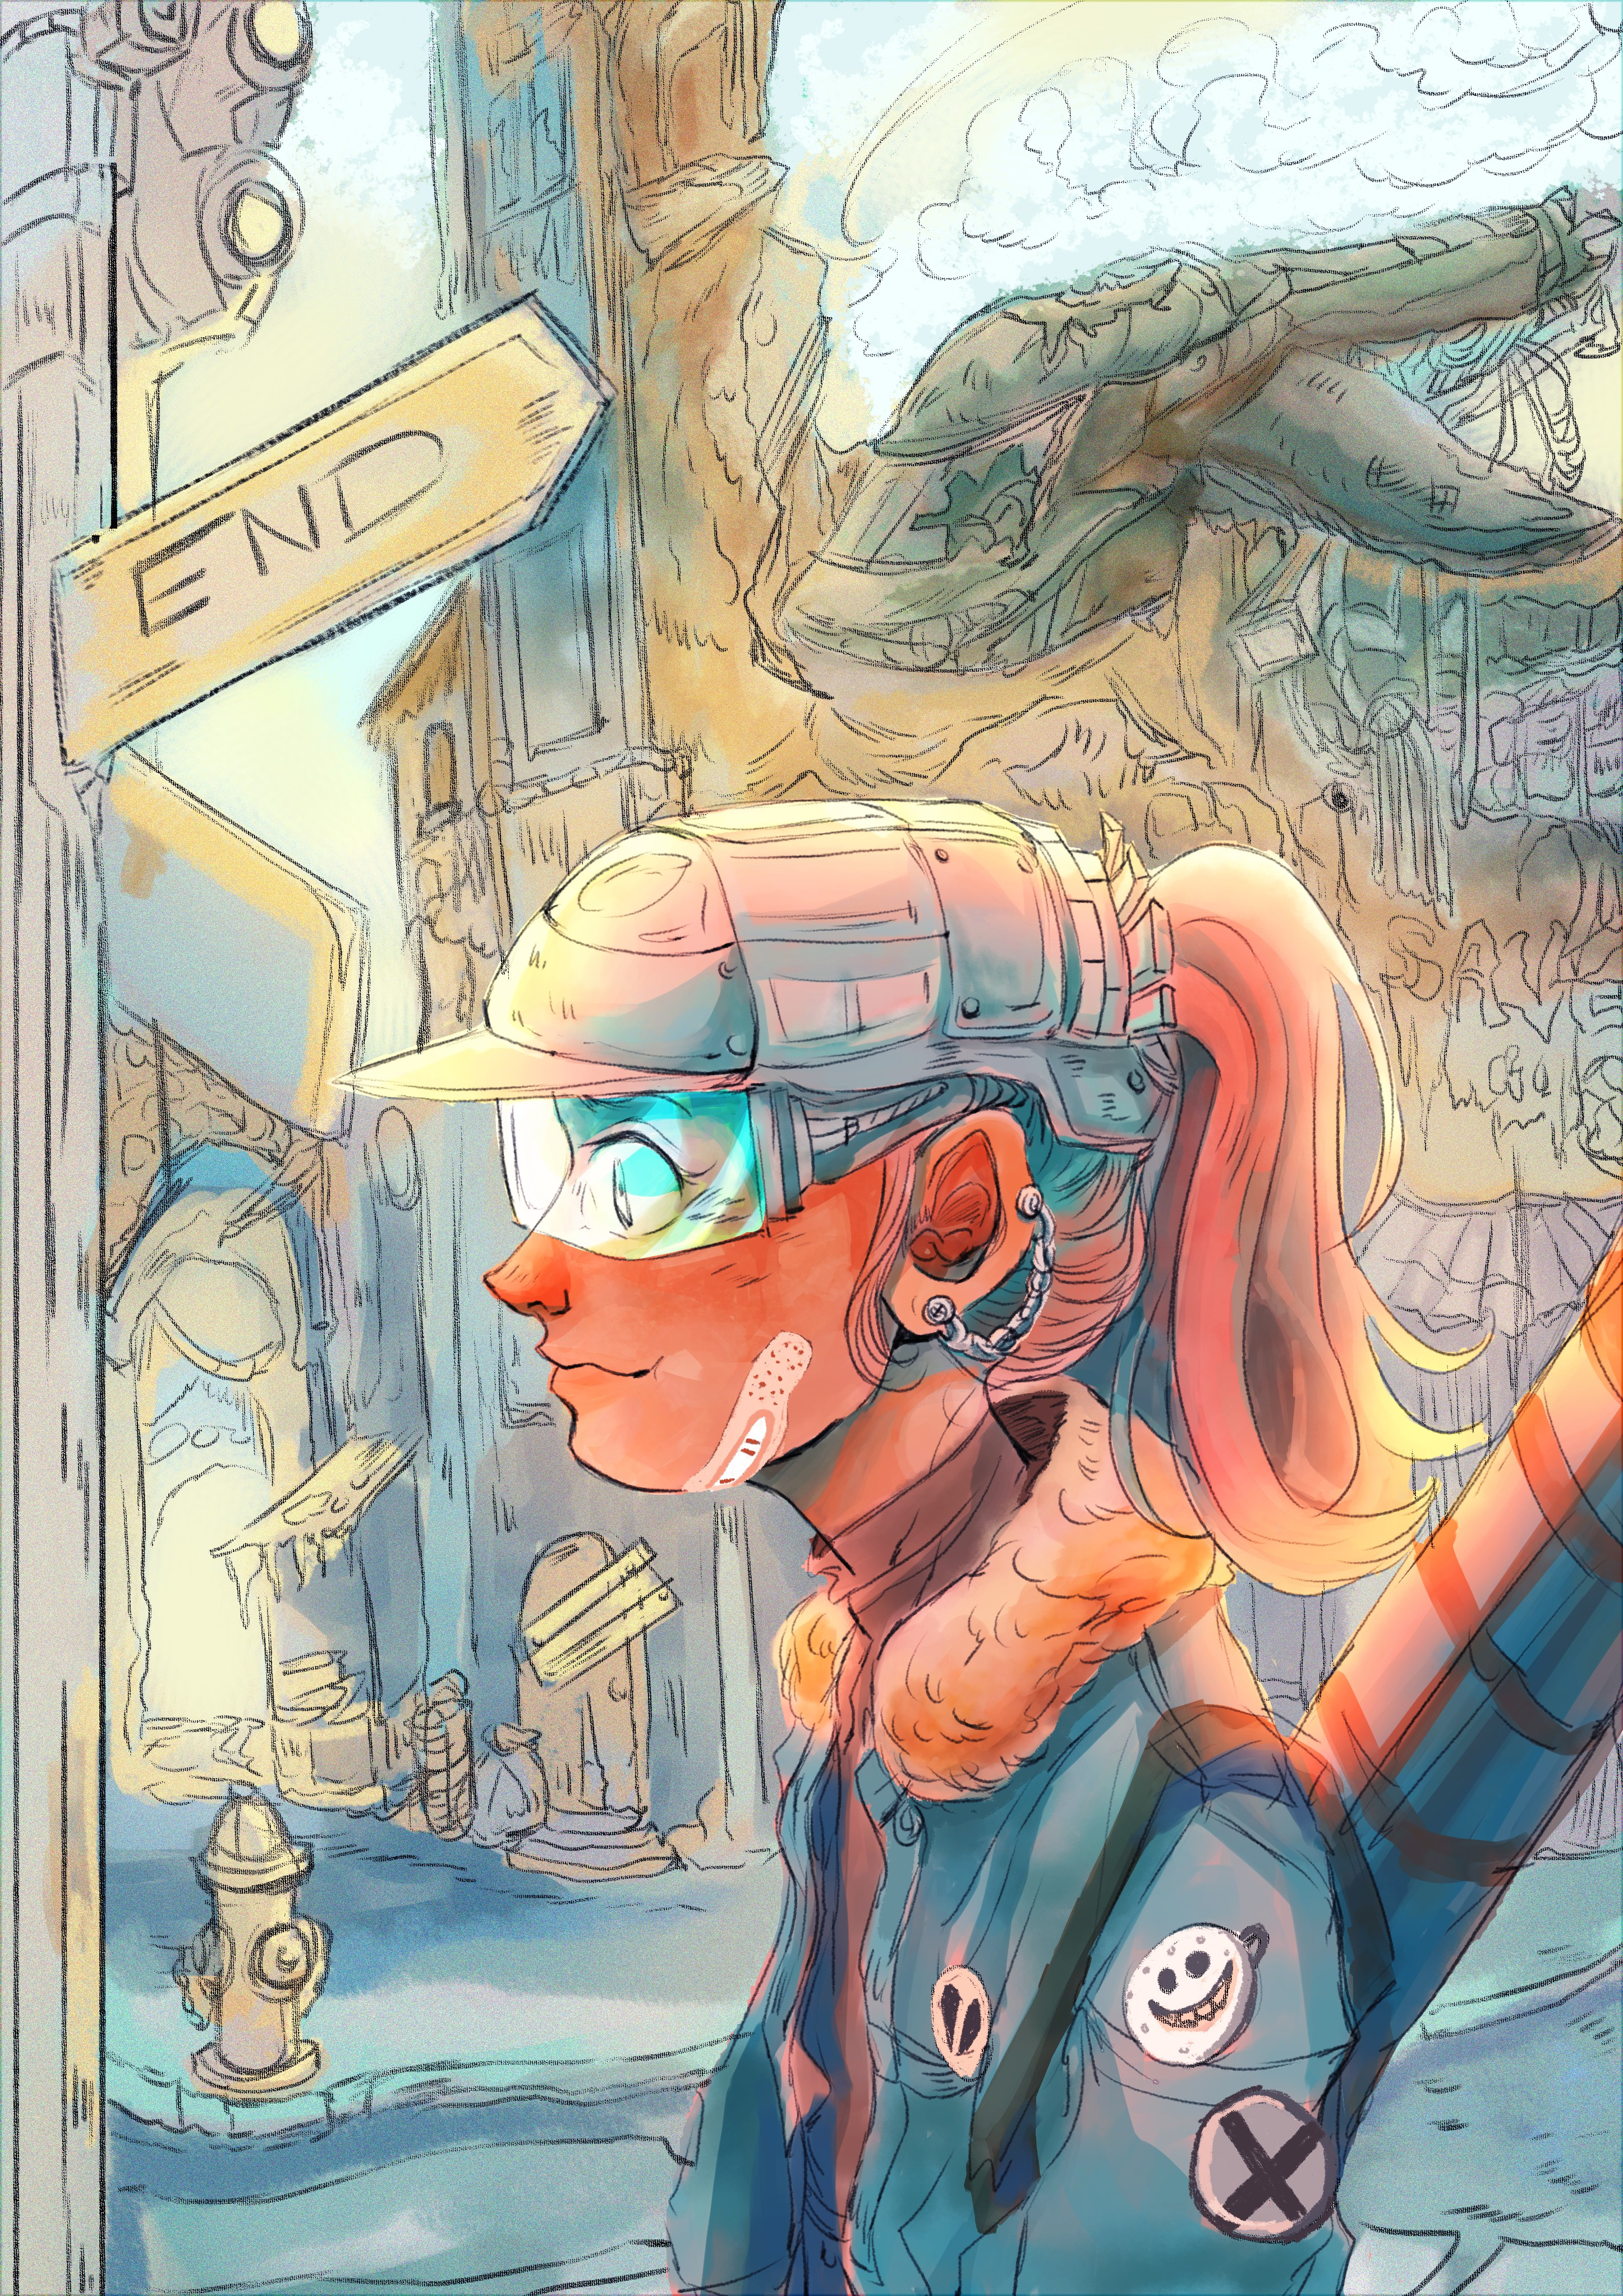
\includegraphics[width=\paperwidth,height=\paperheight,%
				keepaspectratio]{cover01.jpg}}%
			\vfill
}}}
\usepackage{tikz}
\usetikzlibrary{positioning}


%%%%%%%%%%%%%%%%%%%%%%%%%%%%%%%%%%%%%%%%%%%%%%%
\usepackage{tcolorbox}
\usepackage{changepage}
\titlehead{ \texttt{Sistemas Distribuidos} }
\title{\textbf{\texttt{\Huge{INTRODUCCI\'ON  A SISTEMAS DISTRIBUIDOS}}}  } % Title and subtitle
\author{\huge{Virginia Padilla}} 
\publishers{Universidad Nacional Experimental de Guayana}


\definecolor{myorange}{RGB}{244,177,130}
 %%%%%%%%%%%%%%%%%%%%%%%%%%%%%%%%%%%%%%%%%%%%%%%%%%%%%%%

\begin{document}   
		
	%----------------------------------------------------------------------------------------
	%	BOOK INFORMATION
	%----------------------------------------------------------------------------------------

	\AddToShipoutPicture*{\BackgroundPic}	

		\makeatletter
	\renewcommand{\maketitle}{
 	\begin{titlepage}    
		 
		\vspace*{20pt}
		\begin{adjustwidth}{}{-1in}
			\begin{flushright}
				\begin{tcolorbox}[sharp corners,
					rounded corners=northwest, 
					rounded corners=southwest,
					arc=10mm,
					colback=myorange,
					colframe=myorange,
					text width=\dimexpr15cm+1in]
					{\LARGE\@title}
					
					\vspace{30pt}
					
					{\large\@author}
					
					\@date
					
					\vspace{20pt}
				\end{tcolorbox}
			\end{flushright}
		\end{adjustwidth}
 		\end{titlepage}    
  	}                        %%%  <-----------------aquiiiiiii
  	\makeatother
	
	
	%%%%%%%%%%%%%%%%%%%%%%%%%%%%%%%%%%%%%%%%%%%%%%%%%%%%%%%%%%%%%%%%%%%%%%%%%%%%%
 %	\title{ Introducci\'on a los Sistemas Distribuidos }
 

%\subtitle{Introducci\'on}
%\normalfont\texttt
% \author[Virginia Padilla]{Virginia Padilla}
% \author[Virginia Padilla]{Virginia Padilla\thanks{A \LaTeX\ lover}}
 %\date{\today}
%\publishers{1\textsuperscript{era} Edici\'on}

%---------------------------------------------------------------------------------------

%-----------------------------------------------------------------------------

%-----------------------------------------------------------------------------
\frontmatter % Denotes the start of the pre-document content, uses roman numerals


	
	%---------------------------------------------------------------------------------------
	%	COPYRIGHT PAGE en archivo copyright.tex
	%----------------------------------------------------------------------------------------

 
	%----------------------------------------------------------------------------------------
	%	OUTPUT TITLE PAGE AND PREVIOUS
	%----------------------------------------------------------------------------------------
 
	% Note that \maketitle outputs the pages before here
	
	\maketitle
	%----------------------------------------------------------------------------------------
	%	PREFACE
	%----------------------------------------------------------------------------------------
 
 	%\setchapterpreamble[u]{\margintoc}


\makeatletter

% \extratitle{
	% In the title page, the title is vspaced by 9.5\baselineskip
\vspace{1cm}
	%	\vspace*{\parskip}
 	\begin{center}
	 		% In the title page, \huge is set after the komafont for title % 
	 	  	\usekomafont{title}\huge { \@titlehead }
 	 	   \end{center}  
% 	 	}
 	    \makeatother
%---------------------------------------------------------------------------------------
%	COPYRIGHT PAGE
%----------------------------------------------------------------------------------------
 
  	 
 \vspace{14cm}
 
	\small{	
	\textbf{No copyright}\\
	\cczero This book is released into the public domain using the CC0 code. To the extent possible under law, I waive all copyright and related or neighbouring rights to this work.
	
	To view a copy of the CC0 code, visit: \\\url{http://creativecommons.org/publicdomain/zero/1.0/}
	
 \vspace{1cm}
	
	\textbf{Colof\'on} \\
	Este documento fue escrito con la ayuda de
  \href{https://sourceforge.net/projects/koma-script/}{\KOMAScript} y \href{https://www.latex-project.org/}{\LaTeX} usando la clase \href{https://github.com/fmarotta/kaobook/}{kaobook}.
	
	La p\'agina web   de este libro est\'a disponible en: at:\\\url{https://github.com/vpadilla/distribuido}
	
	 \vspace{1cm}
	
	\textbf{Publicado} \\
	Primera impresi\'on en Oct 2023 por Universidad Nacional Experimental de Guayana 
 
}

\newpage
 

 \vspace*{8cm}

 \begin{Huge}
 	{Dedicatoria}
 \end{Huge}
 
 \vspace{1cm}
  
 \begin{Large}
 
 
	\textit{	 
	The harmony of the world is made manifest in Form and Number, and the heart and soul and all the poetry of Natural Philosophy are embodied in the concept of mathematical beauty.\\
	\hspace{4cm}{ -- D'Arcy Wentworth Thompson}
	}
	
\end{Large}
 
 
	\setchapterpreamble[u]{\margintoc}

\chapter{Prefacio}  
 
 El propósito de este documento es  proporcionar un texto gu\'ia al  curso Sistema Distribuido que se imparte en la Universidad Nacional Experimental de Guayana, UNEG, bajo la plataforma Moodle.
 
Este libro electrónico se ha alimentado con las notas  de clase que uso para dictar este curso. Estos apuntes, las he construido revisando y tomando notas de textos actualizados asociados al tema.  Cualquier error u omisión es solo atribuible a mi persona. En caso de que el lector tenga sugerencias o requiera reportar errores, puede escribirme al correo  virginiapadillas@gmail.com.
 

La escritura de este documento se hizo usando  el sistema  tipogr\'afico   \href{https://www.latex-project.org/}{\LaTeX{}} con el documento definido por \href{https://sourceforge.net/projects/koma-script/}{\KOMAScript}   usando la clase \href{https://github.com/fmarotta/kaobook/}{kaobook}. 
Puede consultar la clase    \href{ https://github.com/fmarotta/kaobook} {Kaobook} en GitHub.

Las figuras de las portadas y  encabezados de  capítulos fueron elaborados por Andrea Isabel Revilla.  Pueden ver sus trabajos en  Instagram: \textbf{@ave.rebel}  y en la p\'agina de\textit \textit{ArtStation} \href{https://linktr.ee/avebel}{Avebel}. 
 Por otra parte, las figuras que acompa\~nan los cap\'itulos fueron elaboradas por Ana Virginia Revilla. 


	\index{prefacio}
	
	%----------------------------------------------------------------------------------------
	%	TABLE OF CONTENTS & LIST OF FIGURES/TABLES
	%----------------------------------------------------------------------------------------
	
	\begingroup % Local scope for the following commands
	
	% Define the style for the TOC, LOF, and LOT
	%\setstretch{1} % Uncomment to modify line spacing in the ToC
	\hypersetup{linkcolor=blue} % Uncomment to set the colour of links in the ToC
	\setlength{\textheight}{230\hscale} % Manually adjust the height of the ToC pages
	
	% Turn on compatibility mode for the etoc package
	\etocstandarddisplaystyle % "toc display" as if etoc was not loaded
	\etocstandardlines % "toc lines" as if etoc was not loaded
	
	\tableofcontents % Output the table of contents
	
	\listoffigures % Output the list of figures
	
	% Comment both of the following lines to have the LOF and the LOT on different pages
	\let\cleardoublepage\bigskip
	\let\clearpage\bigskip
	
	\listoftables % Output the list of tables
	
	% Comment both of the following lines to have the LOF and the LOT on different pages
	\let\cleardoublepage\bigskip
	\let\clearpage\bigskip
	
	
	%Lista de Programas
	\lstlistoflistings    % lista de codigos 
	
	\endgroup
	%--------------------------------------------------------------------------------
	%	MAIN BODY
	%--------------------------------------------------------------------------------
	
	\mainmatter % Denotes the start of the main document content, resets page numbering and uses arabic numbers
	\setchapterstyle{kao} % Choose the default chapter heading style
	
	%%\input{chapters/introduction.tex}
	\pagelayout{wide} % No margins
	\addpart{Conceptos y Arquitecturas}
	\pagelayout{margin} % Restore margins
	
	
%\setchapterimage[6cm]{images/cabecera}
%\setchapterpreamble[u]{\margintoc}


\chapter{Introducción a los Sistemas Distribuidos}
\label{cap:def-SD}

\index{sistemas distribuidos}
%\section{ Conceptos}
Un sistema distribuido no solo es una  red de computadora; es una infraestructura conformada por un grupo de computadoras interconectadas por medio de enlaces de comunicación de diversos medios y topologías posibles, y que utilizan un conjunto  de protocolos de comunicación para así mostrar al usuario la percepción de un sistema unificado.

Además de redes de computadoras, las capas adicionales, como el \gls{middleware}, proporcionan  la  integración de  aplicaciones construidas con diversos lenguajes, sistemas operativos y arquitecturas.
  
Los {sistemas distribuidos}  pueden definir  
como: una colección de computadoras independientes que dan al usuario la impresión de constituir un único sistema coherente. 

Esta definición \cite{Steen2017} abarca dos elementos fundamentales:  computadoras y  usuarios o aplicaciones que usan este sistema. El primer elemento  consta de componentes   autónomos; el segundo,  los usuarios (personas o programas) creen que realmente interactúan con un sistema único.  Esto significa que de una manera u otra los componentes autónomos necesitan colaborar entre sí. En la forma de establecer esta colaboración radica  el fondo del desarrollo de los sistemas distribuidos.

De igual manera en  \cite{Verissimo2012},  define a los sistemas distribuidos como un sistema compuesto de varias computadoras las cuales se comunican a través de una red de computadoras, y que alberga procesos que usan un conjunto de protocolos distribuidos comunes, y que proporcionan una ejecución coherente de las actividades distribuidas.

Este concepto destaca los siguientes aspectos: una red de computadoras, los procesos que se ejecutan en esa red, los protocolos  que permiten la comunicación  entre los procesos y la integración de las aplicaciones construidas sobre la red de computadoras. 

Por su parte, en \cite{Coulouris2011}, se define como aquel en el que los componentes de hardware o software están ubicados en una red de  computadoras y, comunican y coordinan sus acciones solo pasando mensajes. Las computadoras que están conectadas por una red pueden estar separadas espacialmente por cualquier distancia, en continentes separados, en el mismo edificio o en la misma habitación.

Esta definición  apunta a lo siguiente:
\begin{description}
	\item[{Concurrencia.}] en una red de computadoras, la ejecución concurrente de programas, es la norma. \index{concurrencia}
	
	\item[{Ausencia de reloj.}]	 No hay una noción global única del tiempo correcto. Esta es una consecuencia directa del hecho de que la única comunicación es enviando mensajes a través de una red.\index{ausencia de reloj}
	
	\item[{Fallas.}] Todos los sistemas informáticos pueden fallar, y es responsabilidad de diseñadores de sistemas  planificar las consecuencias de posibles fallas.  \index{fallas}
\end{description}

\section{ Sistemas Distribuidos vs Centralizados}
Los sistemas distribuidos contrasta con los sistemas de computación tradicionales,  donde una sola computadora ejecuta el software que proporciona un \gls{servicio} , o la computación \gls{cliente-servidor}, donde varias maquinas accesan de manera remota a un servicio centralizado.
En los sistemas distribuidos hay miles o millones de maquinas trabajando juntas para proporcionar un gran servicio. 

\begin{table}[h]\index{centralizado vs distribuido}
	\footnotesize%
	\begin{center}
		\footnotesize
		\begin{tabular}{ll}
			\toprule
			Sistema Centralizado &  Sistema Distribuido \\
			\midrule
			\quad Accesible &  \'Ambito geográfico    \\
			\quad Homog\'eneo    &  Heterogéneos  \\
			\quad Administrable     &  Modular  \\
	%		\quad                    & Escalable \\
%			\quad Consistente & Compartidas   \\
			\quad Consistente   & Degradación elegante \\
			\quad Seguridad  & Seguridad a costo bajo  \\
			\addlinespace 
			\bottomrule
		\end{tabular}
	\end{center}
	\caption{Sistema Centralizados vs Distribuido. \\ Adaptado de \cite{Verissimo2012} }
	\label{tab:centra-dist}
\end{table}

En el cuadro \ref{tab:centra-dist} se muestra algunas de las diferencias entre los sistemas centralizado y distribuido \cite{Verissimo2012}.

\paragraph{Accesible vs Ámbito Geográfico.}
Los sistemas centralizados son  homogéneos  en cuanto a tecnologías y procedimientos; hay un acceso  natural a los \gls{recursos} porque estan constituidos por  sistemas locales.  \index{ámbito geográfico}
Por su parte, los sistemas distribuidos  tienen un alcance geográfico potencialmente más amplio, debido a que se puede operar y acceder de manera remota.  

\paragraph{Homogéneos vs Heterogéneos.}
En cuanto a  tecnologías y procedimientos, los sistemas centralizados son homogéneos ya que sus arquitecturas, protocolos, lenguajes son propios de un tipo de arquitectura; hay un acceso  natural a los \gls{recursos} porque están constituidos por sistemas locales. En cambio, los sistemas distribuidos son heterogéneos ya que poseen diferentes arquitecturas, protocolos y  sistemas operativos. \index{heterogéneos}

\paragraph{Administrable vs Modular}
Los sistemas centralizados son administrables porque estan compuestos por estructuras centralizadas, y debido a ese tipo de estructura logran ser consistentes y seguros. Por su parte, los sistemas distribuidos,  debido a su modularidad,  resultan ser más expansibles y  escalable en cuanto a número de sitios y extensión geográfica.  \index{modular} 

\paragraph{Consistente vs Degradación elegante.}
Es más fácil mantener un sistema coherente en  sistemas centralizados debido a que  su administración es sobre tecnologías y procedimientos homogéneos, y  recursos  constituidos por sistemas locales. 
%%Por su parte, los  sistemas distribuidos deben elegir entre ser consistentes o estar disponibles, por lo que es difícil capturar el estado global del sistema, debido a las potenciales fallas que pueden sufrir.

 

\begin{tcolorbox}
	[colback=red!5!white,colframe=red!75!black,fonttitle=\bfseries,title=Degradación Elegante]
	\gls{degradacion elegante} es el concepto que describe  a sistemas informáticos y de red que pueden operar  de manera progresivamente degradada,  en la medida  que fallan sus componentes, pero sin la ocurrencia de un colapso en el sistema como consecuencia de esas  fallas. Presentado en Emerging resilience techniques for embedded devices, Demara et al, 2017.
\end{tcolorbox}

Los sistemas distribuidos expresan un comportamiento llamado  \texttt{\textbf{degradación elegante}}. Esta característica  potencia que los sistemas distribuidos puedan  lograr confiabilidad y disponibilidad. Y, conjuntamente con la modularidad de los componentes, la separación geográfica,  la redundancia y las técnicas de reconfiguración, logran que los sistemas distribuidos tenga una alta tolerancia a fallos.   
 \index{tolerancia a fallas} 
 \index{confiabilidad} 
 \index{disponibilidad}  
 \index{degradación elegante} 

\paragraph{Seguridad vs Seguridad a bajo costo.}
La  seguridad en los sistemas centralizados  se logra mediante el control de acceso físico y aislamiento.
En cuanto a los sistemas distribuidos, se  puede alcanzar un alto nivel de seguridad con un costo más bajo,  siempre que sea logrado más a costa de reducir el efecto de las intrusiones, que el de las amenazas; esto es debido a lo difícil y costoso que resulta reducir amenazas en sistemas abiertos y públicos. 

\paragraph{Ejemplos de Sistemas Distribuidos} 

Hay una amplia gama de ejemplos en sistemas distribuidos. Muestra de ellos \cite{Coulouris2011}: 
\begin{description}
	\item[{Comercio electrónico y Finanzas}] 
	\index{comercio electrónico} 
	El crecimiento del comercio electrónico, ejemplificado por empresas como Amazon y eBay, y tecnologías de pago como PayPal;  banca y el comercio en línea y sistemas de difusión de información para los mercados financieros.
 	
	\item[{ Industria del Entretenimiento}] \index{juegos en línea} 
	El surgimiento de los juegos en línea,  como una forma novedosa y altamente interactiva de entretenimiento; la disponibilidad de música y películas en el hogar  a través de centros de medios en red e Internet por medio de contenido descargable o en tiempo real;  temas generado por el usuario, por ejemplo a través de servicios como YouTube; nuevas formas de arte y entretenimiento habilitado por tecnologías emergentes.
		
	\item[{Salud}] \index{informática de la salud} 
	El crecimiento de la informática en la salud  como disciplina con su énfasis en 	registros electrónicos de pacientes en l\'inea y cuestiones relacionadas con la privacidad; el papel creciente de la telemedicina en el apoyo al diagn\'ostico remoto o 	servicios avanzados como cirug\'ia remota.
		
	\item[{Educación}] \index{e-learning} 
	La aparici\'on del  \textit{e-learning}  mediante, por ejemplo, herramientas basadas en la web,	como entornos virtuales de aprendizaje; apoyo asociado con la educación a distancia; apoyo para el aprendizaje colaborativo o comunitario.
	
	\item[{Transporte}] El uso de tecnologías  como GPS en sistemas de búsqueda de rutas y gestión de tráfico. Servicios como MapQuest, Google Maps y Google Earth. 
	\index{transporte}
	
	\item [{ Ciencias}] \index{eCiencias}
	El surgimiento de Grid como tecnología fundamental para las eCiencias, 	incluyendo el uso de  redes de computadoras complejas para apoyar el 	almacenamiento, análisis y procesamiento de datos científicos.
	
	\item[ { Gestión Ambiental }] El uso de tecnología de sensores (en red) para monitorear y administrar el medio ambiente natural, por ejemplo, para proporcionar una alerta temprana de desastres naturales como terremotos, inundaciones o tsunamis y para coordinar respuesta de emergencia; la recopilación y el análisis de los parámetros ambientales para comprender mejor los complejos naturales 	fenómenos como el cambio climático. \index{gestión ambiental}
			
\end{description}


%%En el cuadro \ref{tab:Ejemp-dist} se muestra un resumen de los distintos ejemplos de sistemas distribuidos:

%\begin{kaobox}[frametitle= Ejemplos de Sistemas Distribuidos]
		
%%	\begin{table}[h]\index{centralizado!distribuido}
%%		\footnotesize%
%%		\begin{center}
%%			\footnotesize
%%			\begin{tabular}{ll}
%%				\toprule
%%					  &    \\
%%				\midrule
%%				\quad Finanzas y Comercios  &  eCommerce e.g. Amazon, eBay,   \\  				\quad &  PayPal,  banco en 	línea        \\              	
%%				\quad Sociedad de la Informaci\'on  &  Información Web y motores de búsqueda,   \\
%%					\quad &  ebooks,
%%					Wikipedia; Redes sociales:      \\ 				\quad & Facebook y MySpace.   \\
%%				\quad Recreaci\'n y Entretenimiento  &  Juegos en línea, contenido generado por el  \\
%%					\quad &     usuario, 					ej, . YouTube, Flickr      \\
%% 					\quad Cuidado de Salud  &  Registros médicos en línea, monitoreo\\  	\quad &     de pacientes 					e-medicina       \\
%%					\quad Educaci\'on  &  e-learning, ambientes virtuales de \\
%%					\quad &       aprendizaje; 					educación a distancia    \\
%% 		\quad Transporte y Log\'istica  &  GPS en sistemas de búsquedas de rutas,  \\
%%	 	\quad &    servicios	de mapas: Google Maps,\\ 					\quad &  Google Earth      \\  				\quad Ciencia  &  La Grid, tecnología disponible para  			 \\    				\quad &   colaboración 	entre científicos       \\    					\quad Gesti\'on Ambiental  &      					Gestión ambiental Tecnología de sensores \\    						\quad &  para monitorear terremotos,  						inundaciones,       \\  					\quad &  zonas de riesgo, tsunamis   \\	  				 
%%				\addlinespace 
%%				\bottomrule
%%			\end{tabular}
%%		\end{center}
%%		\caption{Ejemplos de Sistemas Distribuidos. \\ Adaptado de \cite{Coulouris2011} }
%%		\label{tab:Ejemp-dist}
%%	\end{table}
%%%%%%% 	
\section{Principios de Dise\~no }
\label{sec:principio-SD}
\index{principios de diseño}

La siguiente secci\'on describe los objetivos  o lo  que debe tomarse en cuenta cuando se  dise\~na un sistema sistema distribuido: \cite{Coulouris2011, Verissimo2012, Limoncelli2014, Steen2017, Deka2017, Czaja2018}

\begin{description} 
	
	\item {\textbf{Concurrencia}.} \index{concurrencia} Tanto los servicios como las aplicaciones proporcionan recursos que los clientes pueden compartir en un sistema distribuido. Por tanto, existe la posibilidad de que varios clientes intenten acceder a un recurso compartido al mismo tiempo. La concurrencia se hace más compleja cuando existen  actividades paralelas que interactúan o comparten los mismos recursos. 
	
	\item {\textbf{Compartir Recursos}.} \index{recursos} Los \gls{recursos}, como los  periféricos,  datos en bases de datos,  bibliotecas, así como los datos (variables/archivos),  no pueden replicar por completo en todos los sitios porque no resulta pr\'actico ni rentable. Estos recursos se distribuyen normalmente por todo el sistema, para que su acceso no se convierta en un potencial cuello de botella.
	Por ejemplo, bases de datos distribuidas como MySQL Cluster o Ethereum, particionar los conjuntos de datos en varios servidores, además de replicarlos en algunos sitios para lograr un acceso rápido y proporcionar un servicio confiable. 

	\item[{\textbf{Transparencia}.}] \index{transparencia}    El objetivo de la \gls{transparencia} es hacer que ciertos aspectos de la distribución sean invisibles para el programador de aplicaciones. Por ejemplo, no necesitan preocuparse por la ubicación o los detalles de cómo otros componentes acceden a sus operaciones, o si serán replicados o migrados. Incluso se pueden presentar fallas en la redes y procesos  en forma de excepciones, pero estas deben poder manejarse.  En el cuadro \ref{tab:tipo-dist} se detallan los niveles de transparencia que se deben tomar en cuenta acompañado de su descripción. \index{niveles de transparencia}
	
	\begin{table}\index{tipos de transparencia} 
		\begin{center}
			\footnotesize		    
				\begin{tabular}{p{0.25\textwidth}p{0.7\textwidth}}
					\toprule
					Concepto &  Descripci\'on \\
					\midrule
					
					\quad {Acceso} & Permitir el acceso con las mismas operaciones   de los recursos locales y remotos.  \\						 
					
					\quad {Ubicaci\'on}  &  Que los recursos sean alcanzados  sin   conocer su ubicación física o de red. \\					
					
					\quad {Red}  &  Combina ambas transparencias: en el acceso  y en  la ubicación.  \\				
					
					\quad {Concurrencia}  & Permite que varios procesos operen  simultaneamente usando recursos compartidos  sin interferencia entre ellos. \\ 
					
					\quad {Replicaci\'on } & Permite que múltiples instancia de recursos  sean usados para aumentar  la confiabilidad  y    rendimiento sin que el usuario  de aplicaciones conozca de ellas.\\ 
					
					\quad {Fallas}  &  Ocultamiento de fallas, permitiendo que    usuarios y aplicaciones culminen sus tareas   sin percatarse de ellas.\\  
					
					\quad{ Movilidad}  & Permite el movimiento de recursos y clientes  dentro del sistema  sin afectar la operación   de usuarios o programas.\\  
					
					\quad {Rendimiento}  &  Permite que el sistema sea reconfigurado  para    mejorar el rendimiento cuando su carga varía.\\ 
					
					\quad {Escalamiento} & Permite que el sistema y la aplicación se    incremente sin cambios   en la estructura   del    sistema o en los algoritmos de aplicación. \\  
				
					\addlinespace 
					\bottomrule
				\end{tabular}
			
				\index{transparencia en el acceso} 
				\index{ transparencia de ubicación}
				 \index{transparencia de red}
				  \index{ transparencia de concurrencia} 
				  \index{transparencia de replicación} 
				  \index{transparencia de fallas}
				   \index{transparencia de movilidad} 
				   \index{transparencia de rendimiento}
				    \index{transparencia de escalamiento}
			\end{center}
			\caption{Tipos de Transparencia. \\ Adaptado de \cite{Steen2017} }
			\label{tab:tipo-dist}
		\end{table}
		
		\item[{Sistemas Abiertos.}] \index{sistemas abiertos} Los \gls{sistemas abiertos}  son aquellos que  puede ampliarse y reimplementarse de varias formas. La apertura  está determinado principalmente por el grado en que los nuevos servicios de intercambio de recursos puede agregarse y estar disponible para su uso por una variedad de programas de cliente.
		Los sistemas abiertos se caracterizan por el hecho de que sus interfaces son públicas; en otras palabras, las aplicaciones proveen un mecanismo de comunicación uniforme e interfaces  publicadas para el acceso a recursos compartidos.
	%%	Los sistemas distribuidos abiertos se pueden construir a partir de hardware  y software heterogéneo, posiblemente de diferentes proveedores. Pero la conformidad de cada componente a la norma publicada debe ser cuidadosamente probado y verificado para asegurar el  funcionamiento correctamente.
		
		\item [{Simplicidad.}] \index{simplicidad} Es importante que un diseño sea lo más simple posible y al mismo tiempo pueda satisfacer las necesidades del servicio ya que los sistemas crecen y se vuelven más complejos con el tiempo. Esto facilita su mantenimiento.
		%% Comenzar con un sistema que ya es complejo significa comenzar en desventaja.	
		%%Proporcionar operaciones competentes requiere tener un modelo mental del sistema en la cabeza. Mientras se trabaja, imaginar el sistema en funcionamiento y usar este modelo mental para rastrear cómo funciona y para depurarlo.  		Cuanto más complejo es el sistema, más difícil es tener un modelo mental preciso. Un sistema demasiado complejo da como resultado una situación en la que ninguna persona lo entiende todo al mismo tiempo.	
		
		\item[{Acoplamiento.}]\index{acoplamiento} 
		
		El grado de \gls{acoplamiento} entre un conjunto de módulos, ya sea hardware o software, se mide en términos de la interdependencia y vinculación y/o homogeneidad entre los módulos. 
		
	 
		
		\begin{tcolorbox}
			[colback=red!5!white,colframe=red!75!black,fonttitle=\bfseries,title=Acoplamiento]
				El concepto de acoplamiento fue presentado por Edward Yourdon en  Structured Design: Fundamentals of a Discipline of Computer Program and Systems Design, Yourdon, 1979.
		\end{tcolorbox}
		
		
		
		 Cuando el grado de acoplamiento es alto, se dice que los módulos están acoplados de manera ajustada o fuerte; por el contrario cuando el grado de acoplamiento es bajo, los módulos están acoplados de manera floja o débil.
		  \index{acoplamiento}   		
		\index{abstracción} 
		Un sistema \gls{debilmente acoplado} facilita la sustitución o adicción de componentes  mientras  está en funcionamiento. Como resultado, un subsistema puede ser reemplazado por uno que proporcione la misma interfaz abstracta incluso si su implementación es completamente diferente. \index{debilmente acoplado}		
		Por el contrario, en  los sistemas  \gls{fuertemente acoplado} es necesario que se compartan recursos comunes, como la memoria central, almacenamiento secundario (disco) y entrada/salida a través de un bus común. \index{acoplamiento fuerte}
		
			
		\begin{tcolorbox}
			[colback=red!5!white,colframe=red!75!black,fonttitle=\bfseries,title=Acoplamiento débil vs fuerte]
			Puede explorar las	diferencias entre el acoplamiento fuerte versus el acoplamiento débil   en este enlace 	\href{https://www.geeksforgeeks.org/difference-between-loosely-coupled-and-tightly-coupled-multiprocessor-system/} {geeksforgeeks}.
		\end{tcolorbox}
		
		 
		
		%%%%%%%%%%%%%%%
		
		\item[{Escalable.}]\index{escalable}   Un sistema se describe como escalable  si permanece efectivo cuando hay un aumento significativo en el número de recursos y el número de usuarios. El diseño de sistemas distribuidos escalable presenta los siguientes retos:		
		%%%%%%%%%%%%%%%%%%%%%%%%%    
		\begin{itemize}			
			\item {Controlar el costo de los recursos físicos}.
			 Es posible ampliar un sistemas, a un costo razonable, a medida que crece la demanda de un recurso.
			
			\item {Controlar la pérdida de rendimiento}. 
			La gestión de un conjunto de datos cuyo tamaño debe ser proporcional al número de usuarios o recursos en el sistema, para evitar el congestionamiento en el acceso a los recursos y afectación del rendimiento.
			
			\item { Evitar cuellos de botella}.
			 En general, los algoritmos deben estar descentralizados para evitar cuellos de botella. Un ejemplo de un problema grave de cuello de botella es el  predecesor del sistema de dominio de nombres \gls{DNS} , en el que la tabla de nombres se mantenía en un archivo maestro único que se podía descargar a cualquier computador. Esto estuvo bien cuando solo había unos pocos cientos de computadoras en internet. Posteriormente,  se eliminó este cuello de botella al dividir la tabla de nombres entre servidores ubicado en Internet y administrado localmente. Ver figura \ref{fig:DNSorg} \index{DNS}
			
			\begin{figure}%
						\begin{center}
				`			\includegraphics[width=0.8\linewidth]{1/DNS.png}
				\caption{Ejemplo de la divisi\'on del espacio de nombres del DNS original a zonas. Tomado de \cite{Steen2017}}
				\label{fig:DNSorg}
						\end{center}
			\end{figure}			
 			
		\end{itemize}
		
		\item[{Heterogeneidad}.] \index{heterogéneos} 
		Los sistemas distribuidos son heterogéneos, ya que se pueden construirse a partir de una variedad de redes, sistemas operativos, hardware informático y lenguajes de programación. Contemplar, por ejemplo, \gls{codigo movil} o \gls{maquina virtual}. El \gls{middleware} se usa para ocultar estar diferencias y permitir la comunicación y administración de datos entre aplicaciones distribuidas.
			
		%%%%%%%%%%%%%%%%%%%%%%%%%%%%%%%%%%
		
		\item[{Seguridad.}] \index{rendimiento} 
		\index{seguridad} \index{confiabilidad} 
		No es suficiente proporcionar acceso a servicios distribuidos. También es importante proporcionar garantías con respecto a cualidades asociadas con dicho acceso al servicio.  Ejemplos de estas caraterísticas incluyen parámetros relacionados con el rendimiento, seguridad y confiabilidad:  En un sistema distribuido, el cliente envia solicitudes de acceso a través de la red a un conjunto de servidores, o almacena sus datos en servicios en la nube. Ambos ejemplos requiere que se construyan aplicaciones seguras donde se protega la información que se envia por la red o la que se almacena en la nube. Este ultimo requerimiento es estudiado por la  criptografía de datos en  bases de datos en la nube.\index{ criptografía de datos}
		
	\end{description}

%%%%%%%%%%%%%%%%%%%%%%%
\section{Teorema CAP.}	\index{teorema CAP} El \gls{Teorema CAP}, inicialmente llamado como la conjetura CAP, recibi\'o el estatus de teorema cuando se proporcion\'o una prueba matem\'atica del concepto, ver \cite{Brewer2000}. 
 CAP establece que en un sistema distribuido, se puede cumplir como m\'aximo con dos de estas propiedades: \gls{consistencia}, \gls{disponibilidad} y \gls{tolerancia de particion}. 

\index{consistencia} En cuanto al concepto de \gls{consistencia}  en aplicaciones distribuidas, por ejemplo, si una empresa usa un servidor de base de datos de respaldo, cuando un usuario actualiza la cuenta de un cliente, esos mismos cambios se realizar\'ian en el servidor de respaldo.

\begin{figure} %
			\begin{center}
	\includegraphics[width=0.8\linewidth]{1/Consistencia.png}
	\caption{Consistencia. Adaptado  de \cite{Sullivan2015} }
	\label{fig:marginCP}
			\end{center}
\end{figure}




Esto requeriría que la base de datos escribiera los datos dos veces: una vez en el disco usado por el servidor primario y luego una vez más en el disco usado por el servidor de respaldo en una operación conocida como confirmación de dos fases, ver Figura \ref{fig:marginCP}. 
Mientras se ejecuta la confirmación de dos fases, se bloquean otras consultas a los datos. Los datos actualizados no estarán disponibles hasta que finalice la confirmación de dos fases. Esto favorece la coherencia sobre la disponibilidad de los datos.


\index{disponibilidad} 
La \gls{disponibilidad} de datos se ilustra en el ejemplo del carrito de compras de comercio electr\'onico \cite{Sullivan2015}, 
donde es posible tener una copia de seguridad de los datos del carrito que no est\'e sincronizada con la copia principal. Los datos seguir\'ian estando disponibles si el servidor primario falla, pero los datos del servidor de respaldo ser\'ian inconsistentes con los datos del servidor primario si el servidor primario falla antes de actualizar el servidor de respaldo.  Ver la Figura \ref{fig:marginAP}.


\begin{figure}%
			\begin{center}
	\includegraphics[width=0.8\linewidth]{1/Disponibilidad.png}
	\caption{Disponiblidad. Tomado de \cite{Sullivan2015} }
	\label{fig:marginAP}
			\end{center}
\end{figure}

El ejemplo m\'as simple de \gls{tolerancia de particion} es cuando el sistema continúa funcionando incluso si las máquinas involucradas en la prestación del servicio pierden la capacidad de comunicarse entre sí debido a que un enlace de red se cae (ver  Figura \ref{fig:marginToleranciaParticion}).

\begin{figure}[H]%
			\begin{center}
	\includegraphics[width=0.8\linewidth]{1/ToleranciaParticion.png}
	\caption{Tolerancia a la Partici\'on. Adaptado de \cite{Limoncelli2014} }
	\label{fig:marginToleranciaParticion}
		\end{center}
\end{figure}
 
La Figura \ref{fig:marginTeoremaCAP} esquematiza estos conceptos y la relaci\'on entre ellos. Alli se resalta los puntos de intersecci\'on entre las propiedades definidas en el teorema, por ejemplo, \texttt{CA} es la intersecci\'on para los sistemas que cumplan la propiedad de consistencia y disponibilidad, \texttt{CP} son los sistemas con las propiedades de consistencia y toleracia a la partici\'on, y \texttt{AP} para las propiedades de disponibilidad y toleracia a la partici\'on.

Noten que la intersecci\'on entre los tres conceptos  no est\'a definida en la Figura \ref{fig:marginTeoremaCAP}. El principio \texttt{CAP} establece que no es posible construir un sistema distribuido que garantice los tres conceptos: consistencia, disponibilidad y tolerancia a la partici\'on. Se pueden lograr uno o dos de ellos, pero no los tres simultáneamente. Al utilizar un sistema distribuidos se debe tener en cuenta qu\'e principios puede garantizar, de acuerdo a su dise\~no. 

\begin{figure}%
			\begin{center}
	\includegraphics[width=0.8\linewidth]{1/TeoremaCAP1.png}
	\caption{ Relaci\'on entre conceptos del Teorema CAP. Adaptado  de \cite{Deka2017}}
	\label{fig:marginTeoremaCAP}
			\end{center}
\end{figure}


En el contexto de una aplicaci\'on de red social global, o un sistema de comercio electr\'onico mundial, la solución deseada es mantener la disponibilidad incluso si se sacrifica cierta consistencia entre los usuarios. Por otra parte, en el sistema financiero mundial, requiere  mantener la consistencia de los datos sobre la disponibilidad de los mismos, por tanto las actualizaciones podr\'ian requerir m\'as tiempo para su ejecuci\'on. 
%%
\begin{figure}
			\begin{center}
	\includegraphics[width=0.8\linewidth]{1/TeoremaCAP.png}
	\caption {Significado del Teorema CAP.}
	\label{fig:TeoremaCAP}
			\end{center}
\end{figure}

En la Figura,  \ref{fig:TeoremaCAP} se muestra las propiedades del Teorema CAP y los tipos de aplicaciones que cumplen con estas propiedades.

%%%%%
	\section{Manejo de Fallas} \index{fallas} 
Los sistemas informáticos a veces fallan. Cuando estas ocurren, ya sea en  hardware o software, los programas pueden producir resultados incorrectos o  detenerse antes de que hayan completado el cálculo.  Las fallas en un sistema distribuido son parciales, es decir, algunos componentes fallan mientras otros continúan funcionando. Por lo tanto, el manejo de fallas es particularmente díficil. 

\index{técnicas contra fallas} Existen técnicas  para lidiar con fallas: detección de la ocurrencia de fallas, enmascaramiento de las fallas, tolerancia a las  fallas, recuperación luego de la ocurrencia de fallas y la redundancia de rutas, caminos o servidores para garantizar funcionamiento de las aplicaciones, a pesar de la fallas. 

En \cite{Gabrielson2019}  
destacan que las fallas en los sistemas distribuidos puede atribuirse a  la complejidad de la ingeniería de los mismos   y se deben a los siguientes motivos: 
	
\begin{tcolorbox}
	[colback=red!5!white,colframe=red!75!black,fonttitle=\bfseries,title=Retos en Sistemas Distribuidos ]
	Puede consultar este documento en \href{https://aws.amazon.com/es/builders-library/
		challenges-with-distributed-systems/} {Retos en SD}
\end{tcolorbox}

\begin{itemize}
	\item { Los ingenieros no pueden combinar las condiciones de error}. En su lugar, deben considerar muchas combinaciones de fallas. La mayoría de los errores pueden ocurrir en cualquier momento, independientemente de cualquiera otra condición de error, por lo que podrían combinarse entre ellos.
	
	\item {El resultado de cualquier operación de red puede ser DESCONOCIDO}. En cuyo caso es posible que la solicitud haya fallado, se haya procesado correctamente o se haya recibido pero no procesado.
	
	\item  {Los problemas distribuidos se producen en todos los niveles}. No solo en los equipos físicos de nivel bajo, sin tembi\'en, en los niveles lógicos del sistema distribuido.
	
	\item {Recursividad}.  Los problemas distribuidos empeoran en los niveles superiores del sistema, debido a la recursividad. 
	
	\item {Aparición del error}. Los errores distribuidos suelen aparecer mucho después de su implementación en un sistema.
	
	\item {Propagación del error}. Los errores distribuidos se pueden propagar en todo el sistema. 
	
	\item  {Origen de la falla}. Muchos de estos problemas provienen de las leyes físicas de las redes, que no se pueden cambiar.
\end{itemize}
%%%%%
Las fallas se caracaterizan como \cite{Coulouris2011}:
	
\begin{description}
	\item[Fallos por omisión] Los fallos clasificados como fallos por omisión se refieren a casos en los que un  proceso o el canal de comunicación no realiza las acciones que se supone que debe realizar
	
	\item [Fallos por omisión del proceso] El principal fallo por omisión de un proceso es que este se bloquee. Un proceso se ha bloqueado cuando se ha detenido y no  ejecutará ning\'un paso de su programa. En los sistemas s\'incronos  el  método de detección de estas fallas se basa en el uso de
	tiempos de espera - es decir, un método en el que un proceso permite un período de tiempo fijo para que  ocurra algo. 
	
	 
	\begin{tcolorbox}
		[colback=red!5!white,colframe=red!75!black,fonttitle=\bfseries,title=Fallas de omisión en sistemas síncronos]
		Por ejemplo, si los procesos $p$ y $q$ están programados para que $q$ pueda responder a un mensaje de $p$, y si el proceso $p$ no ha recibido respuesta del proceso $q$ en un tiempo máximo medido en el reloj local de $p$, entonces el proceso $p$ puede concluir que el proceso $q$ ha fallado.
	\end{tcolorbox}
	
	En un sistema asincrónico, un tiempo de espera puede indicar solo que un proceso no responde: puede que se haya bloqueado o sea lento, o los mensajes pueden que no han llegado.
	
	\item 	[Fallos de omisión de comunicación] Considere las primitivas de comunicación que envían y reciben mensajes. Un proceso $p$ realiza un envío insertando el mensaje $m$ en su buffer de mensaje saliente. El canal de comunicación transporta $m$ al búfer de mensajes entrantes de $q$. El proceso $q$ realiza una recepción tomando $m$ de su búfer de mensajes entrantes y lo entrega (ver Figura \ref{fig:proc-canal} ). Los búferes de mensajes entrantes y salientes son  proporcionado por el sistema operativo.
	
	\begin{figure}%
				\begin{center}
		\includegraphics[width=0.8\linewidth]{1/procesos-canales.png}
		\caption{Procesos y canales.}
		\label{fig:proc-canal}
				\end{center}
	\end{figure}
%\end{description}

	El canal de comunicación produce una falla por omisión si no transporta	un mensaje del búfer de mensajes salientes de $p$ al búfer de mensajes entrantes de $q$. Esto  se debe a la falta de espacio en el búfer en el receptor o en una puerta de enlace intermedia, o por un error de transmisión de red, detectado por un  control de suma (\textit{check sum}) llevada con los datos del mensaje. 


	\item [Fallos arbitrarios]  El término fallo arbitrario o bizantino se utiliza para describir lo peor  falla de  semántica posible , en la que puede ocurrir cualquier tipo de error. Por ejemplo, un proceso puede establecer valores incorrectos en sus elementos de datos, o puede devolver un valor incorrecto en respuesta a un 	invocación.
	Un fallo arbitrario de un proceso es aquel en el que omite arbitrariamente el 	pasos de procesamiento o toma pasos de procesamiento no deseados.  
\end{description}
%%%%%%%%%%%%%%%%%%%%%%%%%%%%%%%%%%%%%%%

\begin{table}[h]\index{middleware}
	\footnotesize%
	\begin{center}
		\footnotesize
		 \begin{tabular}{p{0.18\textwidth}p{0.1\textwidth}p{0.6\textwidth}}
	%	\begin{tabular}{lll}
			\toprule
			Clase de Falla    &  Afecta   & Descripción  \\
			\midrule
			\quad Parada & Proceso & Proceso se detiene y permanece detenido.  Otros procesos pueden detectar este estado. \\
			
			\addlinespace
			\quad 	Bloqueo & Proceso & Proceso se detiene y permanece detenido.  Otros procesos no pueden  detectar este   estado.\\			\addlinespace
			
			\quad Omisión & Canal & Mensaje insertado en un búfer de mensajes  salientes no llega al  b\'ufer de mensajes   entrante del otro extremo  \\
			
			\addlinespace			
			\quad Omisión  Env\'io   & 	Proceso   & Proceso completa una operación de  envío pero el mensaje no se coloca     en su búfer de mensajes salientes.  \\
			
			\addlinespace		
			\quad Omisión  Recepci\'on & Proceso &  Mensaje se coloca en búfer  de mensajes   entrantes de un proceso, pero ese   proceso no lo recibe.  \\
			
			\addlinespace		
			\quad Arbitrario   (Bizantino) &  Proceso   & Proceso/canal muestra un comportamiento  arbitrario:  puede enviar/transmitir  mensajes arbitrarios en momentos arbitrarios o hacer omisiones; puede   detenerse  o tomar un  paso incorrecto. \\
			
			\addlinespace 
			\bottomrule
		\end{tabular}
	\end{center}
	\caption{Tipos de Errores. \\ Adaptado de \cite{Coulouris2011} }
	\label{tab:cat-middle}
\end{table}

\section{Falacias de los sistemas distribuidos}

Las falacias, también nombrado como trampas, son un conjunto de errores o falsas creencias que se cometen al diseñar y desarrollar un  sistemas distribuidos. 


\begin{tcolorbox}
	[colback=red!5!white,colframe=red!75!black,fonttitle=\bfseries,title=Historia de las falacias]
		Peter Deutsch, mientras trabajaba en la empresa Sun Microsystem, en la decada de los 90 propuso la lista de 7 falacias de la computación distribuida; posteriormente, en 1.994, James Gosling, fundador de Java,  añadió una más para finalmente ser conocida como las ocho falacias de los sistemas distribuidos.
\end{tcolorbox}


Las falacias son  \cite{Hoogen2004, Xu2022}:
\begin{description}
	\item \textbf{La red es fiable}.
	 Los sistemas no son inmunes a fallas: los servidores pueden estar fuera de servicio, la energia eléctrica puede fallar. Las aplicaciones deben estar construidas para sortear estas fallas.
	\item \textbf{La latencia es cero}. 
	La \gls{latencia} en redes pequeñas pueden considerarse casi cero; pero en las redes Wan, con servidores remotos, y usuarios alrededor del mundo, la latencia puede ser significativa.
	En estos casos, las aplicaciones deben tener cuidado con las respuestas tardías. Contemplar mecanismos para desechar las solicitudes, hacer reintentos de \gls{peticiones idempotentes}, como mecanismo de prevención de fallas.
	\item \textbf{El ancho de banda es infinito}.
	Así como el ancho de banda aumenta debido a las mejoras de la tecnología, el volúmen de datos se incrementa. Por ello,  podemos  tener problemas con el ancho de banda lo cual influiría en la degradación del rendimiento de la aplicación.
	\item \textbf{La red es segura}.
	Es un error no prestar atención a la seguridad de la aplicación. Las aplicaciones están expuestas a software maliciosos que pueden alterar las funcionalidades del software.
	\item \textbf{La topología no cambia}.
	La red está en cambio constante: nuevas direcciones ip, servidores, dispositivos, servicios, clientes,  entre otros. Los cambios en la topología influye sobre el ancho de banda y el rendimiento de las aplicaciones.	
	\item \textbf{Hay un solo administrador}.
	Un solo administrador es posible en redes pequeñas, pero para  grandes redes, distribuidas geograficamente y con distintos propietarios, esto no se cumple. 
	\item \textbf{El costo de transporte es cero}.
 	En la comunicación entre procesos distribuidos intervienen equipos, sistemas de balance de carga y ancho de banda; en cuanto a la comunicación entre las aplicaciones están involucrado el protocolo que se usa y como se serializa y deserializa.
	\item \textbf{La red es homogénea}.
	Una red homogénea es  pequeña con equipos bajo la misma tecnología, configuración y características. Pero en grandes redes esto no es así: allí se soportan una gran variedad de protocolos y dispositivos, aplicaciones con distintas necesidades y sistemas heterogéneos.
	
	
\end{description}


En la Figura \ref{fig:pitfall} se muestra un esquema con la síntesis de las ocho falacias de los sistemas distribuidos ya referidas.

\begin{figure}%
			\begin{center}
	\includegraphics[width=0.8\linewidth]{1/pitfall.png}
	\caption{Fallas de los Sistemas Distribuidos. Adaptado de \cite{Xu2022} }
	\label{fig:pitfall}
			\end{center}
\end{figure}
%%%%
En resumen, diseñar una aplicación es una tarea que requiere considerar aspectos que están fuera del alcance del diseñador de la aplicación; por ello el proceso de diseño requiere que se haga un ejercicio de escenarios probables de funcionamiento para determinar si la aplicación puede seguir operando a pesar de las posibles escollos que encuentre.
%%%%%
%%\section{Ejercicios}
%\label{sec:ejercicios}

%%\begin{kaobox}[frametitle=Ejercicios ]
%%	\begin{enumerate}

%%\item  Proporcione cinco tipos de recursos de hardware y cinco tipos de datos o recursos de software que puedan ser compartido de manera útil. Dé ejemplos de cómo se comparten  en sistemas distribuciones en la practica.

%%\item Enumere los tres componentes principales de software que pueden fallar cuando un proceso cliente invoca un objeto en el  servidor, dando un ejemplo de falla en cada caso. Sugiera cómo los componentes se pueden fabricar para tolerar las fallas de los demás componentes.

%%\item Los recursos en la World Wide Web y otros servicios se nombran por URL. ?` Qué denotan las iniciales URL ? Dé ejemplos de tres tipos diferentes de recursos web que pueden nombrados por URL.

%%\item  Dé un ejemplo de una URL HTTP. Enumere los componentes principales de una URL HTTP, indicando  sus límites e ilustrando cada uno de ellos a partir de su ejemplo.  
%%\end{enumerate}

%%\end{kaobox}

%%%%%%%%%%%%%%%%%%%%%%%%%%%%%%%%%%%%%%%%%%%%%
\section{Caso de Estudio: Tecnología Web}
\index{caso de estudio!tecnología web}
\label{sec:caso-estudio:web}

La Web es un sistema abierto que se  caracteriza por \cite{Coulouris2011}: a) Su funcionamiento está basado en estándares de comunicación y contenido o en documentos que se publican e implementan libremente. Ejemplo, hay varios tipos de navegador,  implementado en distintas plataformas; así como  implementaciones de servidores web. b) La Web está abierta con respecto a los tipos de \gls{recursos} que se pueden publicar y compartir. Los navegadores están diseñados para adaptarse a nuevas funcionalidades de presentación de contenido en forma de aplicaciones auxiliares y complementos o \textit{plug-ins}.

La Web se basa en  componentes tecnológicos que son  estándares de la W3C, \cite{W3C2022} y que se describen en esta parte. Se presentan una introducción a las siguientes tecnolog\'ias que se usan  en la web: HTTP, HTML, CCS, JavaScript.

\subsection{HTTP}   \index{HTTP} 
HTTP (HyperText Transfer Protocol), \gls{HTTP} es el protocolo usado cuando se visita cualquier sitio web desde un navegador (\textit{browser}). Es un protocolo confiable que facilita la transferencia de información en la web. Esta característica de fiabilidad es  debido a que HTTP utiliza protocolos de transmisión de datos confiables, garantiza que sus datos no se dañarán ni se codificarán durante el tránsito, incluso cuando provengan del otro lado del mundo \cite{W3C2022}, \cite{Gourley2002},  \cite{Allen2017}.

 
\begin{tcolorbox}
	[colback=red!5!white,colframe=red!75!black,fonttitle=\bfseries,title=HTTP]
	Conozca m\'as de HTTP visitando este sitio  \href{https://www.w3.org/Protocols/}{HTTP}
\end{tcolorbox}

	\subsubsection{Clientes y Servidores Web}   \index{Hcliente}   \index{servidor web}
	El contenido de la  web está almacenado en un \gls{servidor web}. Los servidores web usan el protocolo HTTP, por lo que a menudo se les llama servidores HTTP. Estos servidores almacenan los datos de Internet y proporcionan los datos cuando los solicitan los clientes HTTP. Los clientes envían solicitudes HTTP a los servidores y los servidores devuelven los datos solicitados en respuestas HTTP, como se muestra en la Figura \ref{fig:CSweb}. 
	
	\begin{figure} %
				\begin{center}
		\includegraphics[width=0.8\linewidth]{1/Cliente-WebServer}
		\caption{Cliente y Servidor Web}
		\label{fig:CSweb}
				\end{center}
	\end{figure}
	
	
	\subsubsection{Recursos}   \index{recursos}
	Los servidores web alojan \gls{recursos}. Un recurso web es la fuente del contenido web. El tipo más simple de recurso web es un archivo estático en el sistema de archivos del servidor web: pueden ser archivos de texto, archivos HTML, archivos de Microsoft Word, archivos de Adobe Acrobat, archivos de imagen JPEG, archivos de película AVI o cualquier otro formato, ver Figura \ref{fig:CS-Recursos}.
	
		\begin{figure} [h] %
					\begin{center}
		\includegraphics[width=0.8\linewidth]{1/Recursos}
		\caption{Clientes, Servidor Web y Recursos }
		\label{fig:CS-Recursos}
				\end{center}
	\end{figure}

	Los recursos también pueden ser programas de software que generan contenido bajo demanda. Estos recursos de contenido dinámico pueden generar contenido en función de su identidad, de la información que haya solicitado o de la hora del día, por ejemplo videos, transacciones de comercio electrónico, transacciones bancarias, entre otros
	

	
	\subsubsection{MIME}  \index{MIME}
	Debido a que Internet alberga  miles de tipos de datos diferentes, HTTP etiqueta  cada objeto que se transporta a través de la Web con una etiqueta de formato de datos denominada tipo MIME. \gls{MIME} o \textit{Multipurpose Internet Mail Extensions}(en español, Extensiones de correo de Internet multipropósito) se diseñó originalmente para resolver los mensajes entre los sistemas de correo electrónico. HTTP lo adoptó para describir y etiquetar su propio contenido multimedia.
	
	Los servidores web adjuntan un tipo MIME a todos los datos de objetos HTTP. Cuando un navegador web recupera un objeto de un servidor, mira el tipo MIME asociado para ver si sabe cómo manejar el objeto. La mayoría de los navegadores pueden manejar cientos de tipos de objetos populares: mostrar archivos de imagen, analizar y formatear archivos HTML, reproducir archivos de audio a través de los parlantes de la computadora o iniciar software de complemento externo para manejar formatos especiales, entre otros
	
	\subsubsection{URL}
	 \index{URL} 
	 Los navegadores examinan las \gls{URL}	  para acceder a las correspondientes recursos. A veces, el usuario escribe una \textit{URL} en el navegador, o el  navegador busca la \textit{URL} correspondiente cuando el usuario hace clic en un enlace o selecciona uno de sus marcadores o \textit{bookmarks}.
	
 
	\begin{tcolorbox}
		[colback=red!5!white,colframe=red!75!black,fonttitle=\bfseries,title=URL]
			Conozca m\'as de URL visitando este sitio
		\href{https://www.w3.org/TR/url/}{URL}
	\end{tcolorbox}
	
	Ejemplo de las partes de un \textit{URL} se esquematiza en la Figura\ref{fig:URL-HowWork}: 
	
	\begin{figure} %
				\begin{center}
		\includegraphics[width=0.8\linewidth]{1/URL.jpg}
		\caption{Partes de un URL }
		\label{fig:URL-HowWork}
				\end{center}
	\end{figure}

\begin{itemize}
	\item Esquema: es el protocolo usado para realizar la solicitud. Puede ser sin seguridad (http), encriptado (https) y para transferencia de archivos (ftp).
	\item Dominio: donde se envía la solicitud. En las solicitudes de tipo HTTP, el nombre del servidor de destino (host) se fija con este valor.
	\item Puerto: por defecto 80 para HTTP y 443 para HTTPS.
	\item Camino: es la dirección que se debe seguir en el servidor.
	\item Consulta: parámetros de consulta usados para especificar la página que se solicita.
	\item Fragmento: no es enviado en la solicitud al servidor. Se usa para buscar una etiqueta en el documento HTML o por un programa JavaScript en la página.
\end{itemize}
 

	\subsubsection{Transacciones HTTP} \index{transacción}
	Una transacción HTTP consta de un comando de solicitud (enviado del cliente al servidor) y un resultado de respuesta (enviado del servidor al cliente). Esta comunicación ocurre con bloques de datos formateados llamados mensajes HTTP, como se ilustra en la Figura \ref{fig:URL-tran}
	
	\begin{figure} %
				\begin{center}
		\includegraphics[width=0.8\linewidth]{1/URL-tran}
		\caption{Transacción HTTP }
		\label{fig:URL-tran}
				\end{center}
	\end{figure}
	
	\subsubsection{Métodos HTTP}  \index{métodos}
         HTTP proporciona  comandos de solicitud diferentes, llamados métodos HTTP. Cada mensaje de solicitud HTTP tiene un método. El método le dice al servidor qué acción realizar (obtener una página web, ejecutar un programa de puerta de enlace, eliminar un archivo, etc.). En la tabla \ref{tab:met-Http} hay una muestra de cuatro de ellos.

\begin{table}[H]
	\footnotesize%
	\begin{center}
		\footnotesize
		\begin{tabular}{ll}
			\toprule
			Método    &  Descripción    \\
			\midrule
			\quad GET  & Enviar nombre del recurso desde el servidor al cliente. \\  \\		\quad PUT  &  Almacenar datos del cliente en el recurso de destino. \\ \\	
			\quad DELETE & Borra  un recurso en específico. \\  \\	
			\quad POST & Envíar los datos del cliente a una aplicación en la \\ 
			\quad & puerta de enlace del servidor. \\				 
			\addlinespace 
			\bottomrule
		\end{tabular}
	\end{center}
	\caption{Métodos Http }
	\label{tab:met-Http}
\end{table}

\subsection{HTML}  
\index{HTML} 
El lenguaje de marcado de hipertexto, \gls{HTML} se utiliza para especificar el texto e imágenes que componen el contenido de una página web, y  cómo se colocan y formatean,  para su presentación al usuario. \textit{HTML} también se utiliza para especificar enlaces y  recursos que están asociados a ellos. \cite{W3C2022}

 
\begin{tcolorbox}
	[colback=red!5!white,colframe=red!75!black,fonttitle=\bfseries,title=HTML]
	Conozca m\'as de HTML visitando este sitio  \href{https://www.w3.org/html/}{HTML}
\end{tcolorbox}


A continuación, se muestra un fragmento  de texto \textit{HTML}, ver :

     \lstinputlisting[caption=Ejemplo programa en HTML]{C:/Users/virgi/OneDrive/Desktop/book/hello.html} \label{prog:HTML-1}


En el listado \ref{prog:HTML-1} del programa se puede distinguir las siguientes partes:
\begin{itemize}
	\item  La declaración <!DOCTYPE html> indica que este documento es un documento HTML5.
	\item El elemento <html> es el elemento raíz de una página HTML.
	\item El elemento <head> contiene metainformación sobre la página \textit{HTML}.
	\item El elemento <title> especifica un título para la página \textit{HTML} (que se muestra en la barra de título del navegador o en la pestaña de la página).
	\item El elemento <body> define el cuerpo del documento y es un contenedor de todos los contenidos visibles, como encabezados, párrafos, imágenes, hipervínculos, tablas, listas, etc.
	\item El elemento <h1> define un encabezado grande.
	\item El elemento <p> define un párrafo.
\end{itemize}

Un documento \textit{HTML} proporciona tres conceptos: etiqueta, atributo y valor.

\begin{itemize}
	\item Etiqueta: las etiquetas comparten el mismo formato: empiezan con el signo menor que "<" y terminan con el signo mayor que ">". 	Por ejemplo, el elemento html tiene dos etiquetas: etiqueta de inicio <html>   del documento \textit{HTML} y la etiqueta de cierre \textit{</html>} que indica el final del documento \textit{HTML}.
	
	\item Atributo: Son las propiedades que se le pueden asignar a los elementos. Su formato es  \textit{<elemento atributo='valor'> ... </elemento> }.
	\item Valor: es la cualidad asignada al atributo. Ejemplo:  \textit{<html lang='es'> ... </html>} indica el idioma en que está escrito el documento (lang) y el valor asignado es un código de idioma ("es" para el español).
\end{itemize}

Para ejecutar un documento HTML, solo abra el documento con el navegador de su preferencia;
obtendría la siguiente Figura \ref{fig:HTML-1}

	\begin{figure} %
				\begin{center}
	\includegraphics[width=0.8\linewidth]{1/HTML-1.jpg}
	\caption{Hola Mundo}
	\label{fig:HTML-1}
			\end{center}
\end{figure}

\subsubsection{CSS} 
\index{CSS}
\textit{CSS} es la abreviación para referirse a las hojas de estilo en cascada (Cascading Style Sheets), estas se utilizan  para dar formato a las páginas web. Por ejemplo, \gls{CSS}
se puede utilizar para definir el color, el ancho, la altura, los márgenes, la opacidad, el relleno, entre otros atributos. etc.
Usemos el programa \ref{prog:HTML-1} para mostrar como podemos incluir formato en la p\'agina Hola Mundo. 

 Escriba el programa \ref{prog:css-1} y guardelo como \textit{app.css} en una carpeta  llamada \textbf{css}. El programa tiene tres parte: la primera asigna color al fondo de la página, la segunda parte esta dedicada a colorear los elementos marcados con la etiqueta \textit{<h1>}, y en la tercera parte se le asigna color a los elementos contenidos en la etiqueta \textit{<p>}.
 
     \lstinputlisting[caption=Hoja de estilo app.css]{C:/Users/virgi/OneDrive/Desktop/book/html/css/app.css} \label{prog:css-1}
    
     Incluya en el programa Hola Mundo  la siguiente línea  \textit{<link rel="stylesheet" href="css/app.css">}, dabajo de la etiqueta \textit{title}
     
     El programa Hola Mundo modificado se muestra en \ref{prog:Hello2}. 
     
    \lstinputlisting[caption= Hola Mundo con llamada a css]{C:/Users/virgi/OneDrive/Desktop/book/html/hello.html} \label{prog:Hello2}
 
 El programa Hola Mundo tiene ahora la siguiente salida, como puede ver en la Figura \ref{fig:HTML-2}. 
 
 \begin{figure} %
 			\begin{center}
 	\includegraphics[width=0.8\linewidth]{1/HTML-2.jpg}
 	\caption{Hola Mundo con hoja de estilo css}
 	\label{fig:HTML-2}
 			\end{center}
 \end{figure}


 Hay tres formas de implementar una hoja de estilo \textit{CSS} en un programa \textit{HTML}: interno, externo, y archivo en línea. 
\begin{itemize}
	\item Interno en una etiqueta: se añade una etiqueta \textit{<etiqueta style="">} en el programa \textit{HTML} con la definición del estilo. 
	\item Externo: En la sección \textit{<head>} de la página se puede incluir una etiqueta \textit{<style>} que integre todas las reglas de estilo de la página.
	\item Archivo: Mediante la etiqueta \textit{<link>} se puede incluir un fichero externo que incluya todas las reglas.
\end{itemize}
 
 
 En el primer caso sólo se deben especificar los estilos que se aplicarán al elemento en cuestión. Mientras que en los otros dos es necesario especificar, además, a qué elementos de la página se aplicarán los estilos. El último caso es el  mostrado en esta sección. 
 
  
 
 \begin{tcolorbox}
 	[colback=red!5!white,colframe=red!75!black,fonttitle=\bfseries,title=CSS]
 		Puede ampliar el tema de CSS y crear otros estilos revisando esta página  \href{https://www.w3.org/Style/CSS/}{CSS}
 \end{tcolorbox}
 
 Puede ampliar  este tópico y crear otros estilos revisando la siguiente bibliografía referida en la nota al margen del texto y en \cite{DuRocher2021,Shaw2017}.
 

 
\subsubsection{XHTML} 
\index{XHTML}

\textit{XHTML} significa lenguaje de marcado de hipertexto extensible (eXtensible HyperText Markup Language). Es una versión diferente de \textit{HTML}, basada en \textit{XML}. \textit{XHTML} se usa para hacer páginas web y tiene una forma muy específica de escribirse para que sea correcto y sin errores. \textit{XHTML} también distingue entre mayúsculas y minúsculas. Las etiquetas están escritas en minúsculas y deben cerrarse. El orden de las etiquetas también debe estar en el orden correcto para que la información salga correcta. Hay tres secciones principales de XHTML que consisten en una \textit{declaración de declaración}, una \textit{declaración principal} y un \textit{cuerpo}, \cite{Pfaffenberger2004,Musciano2002}.

Un documento \textit{XHTML} se compone de cuatro componentes:

\begin{itemize}
	\item Definición de tipo de documento (DTD): La DTD describe el idioma o la gramática en la que se ha codificado el texto. Es opcional en \textit{HTML}, pero en \textit{XHTML} es requerido.  Pueden ser de tipo \textit{Strict} (no soporta etiquetas antiguas y el código debe estar escrito correctamente), \textit{Transitional} (como XHTML Strict DTD, pero las etiquetas en desuso están permitidas) y \textit{Frameset}(la única DTD XHTML que soporta Frameset, que divide el espacio del documento) donde haya sido insertado, y permite la carga de otros documentos en cada espacio.
	\item Contenido de texto: los encabezados y párrafos que aparecen en la página.
	\item Referencias: contenido avanzado como enlaces e imágenes.
	\item Mark-Up: Instrucciones sobre cómo se debe mostrar el contenido.
\end{itemize}
Cada uno de estos componentes  puede guardarse en formato de texto y verse en cualquier navegador.  
Para adaptar un documento HTMl a XHTML solo debe agregar al inicio del programa el DTD, ver programa \ref{prog:XHTML}
 
     \lstinputlisting[caption=Hola Mundo con HTML y CSS]{C:/Users/virgi/OneDrive/Desktop/book/html/xhtml/hello.html} \label{prog:XHTML}
     
     La diferencia de \textit{XHTML} versus \textit{HTML} son las siguientes:
     
     \begin{itemize}
     	\item <!DOCTYPE> es obligatorio
     	\item El atributo xmlns en <html> es obligatorio
     	\item <html>, <head>, <title> y <body> son obligatorios
     	\item Los elementos siempre deben estar correctamente anidados
     	\item Los elementos siempre deben estar cerrados.
     	\item Los elementos siempre deben estar en minúsculas
     	\item Los nombres de los atributos siempre deben estar en minúsculas.
     	\item Los valores de los atributos siempre se deben citar.
     	\item La minimización de atributos está prohibida.
     \end{itemize}

 Est proporciona las siguientes ventajas en el uso de \textit{XHTML}: 1) Se pueden incorporar elementos de distintos espacios de nombres XML (como MathML y Scalable Vector Graphics). 2)  Un navegador no necesita implementar heurísticas para interpretar el texto por lo que el \textit{parser} puede ser mucho más sencillo. Y 3) Se pueden utilizar fácilmente herramientas creadas para procesamiento de documentos XML genéricos (editores, XSLT, entre otras).

\subsubsection{Páginas Dinámicas}  
\index{script} \index{página dinámica} \index{página estáticas} 

Las páginas dinámicas  \cite{Hoffer2016,Limoncelli2014} son páginas \textit{HTML} generadas a partir de lenguajes de programación \textit{(\gls{scripts})} que son ejecutados en el propio servidor web. A diferencia de otros scripts, como  \textit{JavaScript}, que se ejecutan en el propio navegador del usuario, los scripts en el lado del servidor (\textit{'Server Side' scripts})  generan un código \textit{HTML} desde el propio servidor web. 

Por su parte, las páginas estáticas no son  páginas sin movimientos, son páginas que permanece tal y como fue diseñada. Sin embargo, una página web estática también puede proporcionar una experiencia de usuario "en vivo", "dinámica" o "interactiva". El contenido (texto, imágenes, campos de formulario, etc.) en una página web puede cambiar, en respuesta a diferentes contextos o condiciones.

Estos comportamientos se explican de la siguiente manera:

\begin{itemize}
	\item \gls{pagina estatica}. Uso de secuencias de comandos del lado del cliente para cambiar los comportamientos de la interfaz dentro de una página web específica, en respuesta a las acciones del ratón o \textit{mouse}, o del teclado o en eventos de tiempo específicos. En este caso, el comportamiento dinámico ocurre dentro de la presentación. 
	\item \gls{pagina dinamica}. Uso de secuencias de comandos en el lado del servidor para cambiar la fuente de la página proporcionada entre páginas, ajustando la secuencia o recarga de las páginas web o el contenido web proporcionado al navegador. Las respuestas del servidor pueden estar determinadas por condiciones tales como datos en un formulario HTML publicado, parámetros en la URL, el tipo de navegador que se utiliza, el paso del tiempo o una base de datos o el estado del servidor.
\end{itemize}

Sin embargo, si un usuario  que envía una solicitud de página web no sabe si la solicitud que se envía se está devolviendo a una página web estática o una página web cuyo contenido es una mezcla de información estática y dinámica recuperada de una base de datos \cite{Hoffer2016}.
En la Figura \ref{fig:sol-pag-din} se ilustra cómo es el tratamiento de la información cuando se realiza un requerimiento al servidor.

 \begin{figure} %
 			\begin{center}
	\includegraphics[width=0.8\linewidth]{1/sol-pag-dinamica}
	\caption{Solicitud página estática y página dinámica. Adaptado de \cite{Hoffer2016}}
	\label{fig:sol-pag-din}
			\end{center}
\end{figure}


%Este código HTML puede ser modificado -por ejemplo- en función de una petición realizada por el usuario en una Base de Datos. Dependiendo de los resultados de la consulta en la Base de Datos, se generará un código HTML u otro, mostrando diferentes contenidos.  \cite{Owen2022}.   Gran parte de la experiencia de los usuarios en la Web es el de interactuar con los servicios en lugar de recuperar datos. Por ejemplo, cuando se compra un artículo en una tienda en línea, el usuario  completa un \gls{formulario web} para proporcionar datos personales o para especificar  lo que se desea comprar.  Cuando el usuario envía el formulario, el navegador envía una solicitud \textit{HTTP} a un servidor web, que contiene los valores que el usuario ha ingresado. 

%Dado que el resultado de la solicitud depende de la entrada del usuario, el servidor debe procesar la entrada del usuario. Por lo tanto, la \textit{URL} o su componente inicial designa un 	programa en el servidor. 	Si la entrada del usuario es un conjunto  pequeño de 	parámetros,  se envía como el componente de consulta de la \textit{URL}, utilizando m\'etodo \textit{GET} o alternativamente, se envía como datos adicionales en la solicitud utilizando el m\'etodo \textit{POST}.
%%%%%
\paragraph{JavaScript} 
\index{JavaScript}

Javascript es el lenguaje de programación de la Web \cite{Flanagan2006}. \gls{JavaScript} es  un lenguaje interpretado que es ejecutado por el navegador que utilizamos para ver las páginas. Eso hace posible  desarrollar páginas dinámicas de muy diverso tipo, desde generadores de HTML, comprobadores de formularios, hasta programas que gestionen las capas de una página .  

También se puede usar para actualizar partes del contenido de una página web sin
obtener una versión completamente nueva de la página y volver a renderizarla. Estas actualizaciones dinámicas pueden ocurrir ya sea debido a una acción del usuario , o cuando
el navegador adquiere nuevos datos del servidor que suministró la página web. 
En este ultimo caso,  el momento de la llegada de los datos no está relacionado con ninguna acción del usuario en el propio navegador, por ello se denomina asíncrono. Una técnica conocida como \textit{AJAX}  se utiliza en tales casos.

 
\begin{tcolorbox}
	[colback=red!5!white,colframe=red!75!black,fonttitle=\bfseries,title=JavaScript]
	Una breve historia de JavaScript en este vídeo \href{https://www.youtube.com/watch?v=i18gWXhv5aA}{JavaScript}
\end{tcolorbox}


\paragraph{AJAX}
\index{AJAX}
 

\textit{Ajax} (Asynchronous JavaScript and XML) \cite{Asleson2005} se refiere a un grupo de tecnologías que se utilizan para desarrollar aplicaciones web. Al combinar estas tecnologías, las páginas web son más receptivas puesto que los paquetes  de datos que se intercambian con el servidor y las páginas web no se vuelven a cargar cada vez que un usuario realiza un cambio de entrada. 

El término \textit{Ajax}  proviene de la agrupación de las tecnologías que lo sustentan \cite{Gehtland2006}: 
\begin{enumerate}
	\item un canal de comunicación asíncrono entre el navegador y el servidor.
	\item JavaScript y XML.
\end{enumerate}

\textit{Ajax} se compone de las siguientes tecnologías:

\begin{itemize}
    \item Presentación basada en estándares usando XHTML y CSS.
    \item Visualización dinámica e interacción utilizando el \textbf{Modelo de Objetos del Documento} (\gls{DOM}, Document Object Model) del navegador. 
	\item  Intercambio y manipulación de datos mediante XML y XSLT.
	\item Recuperación asíncrona de datos usando el objeto \gls{XMLHttpRequest}.
	\item JavaScript que une todo.
\end{itemize}
%%%%
En la Figura \ref{fig:AJAX} se muestra como encajan estas tecnologías \cite{Crane2005}.  JavaScript  mantiene unida la aplicación, definiendo el flujo de trabajo del usuario y la lógica de negocio. La interfaz de usuario se manipula y actualiza
mediante el uso de JavaScript para gestionar el modelo de objetos de documento (DOM), redibujando y reorganizando continuamente los datos presentados a los usuarios y procesando sus interacciones basadas en el mouse y en el teclado. Las hojas de estilo en cascada (CSS) brindan una apariencia consistente a la aplicación  para la manipulación  del DOM. El objeto \textit{XMLHttpRequest}  se utiliza para hablar con el servidor de forma asincrónica, ejecutando las solicitudes de los usuarios y la obtención de datos actualizados mientras el usuario continúa operando. 

 \begin{figure} %
 			\begin{center}
	\includegraphics[width=0.8\linewidth]{1/AJAX}
	\caption{Componentes de AJAX. Adaptado de \cite{Crane2005}}
	\label{fig:AJAX}
		\end{center}
\end{figure}


En una aplicación web tradicional, las solicitudes HTTP que se inician mediante la interacción del usuario con la interfaz web, se envía a un servidor web. El servidor web procesa la solicitud y devuelve una página HTML al cliente. Durante el transporte HTTP, el usuario no puede interactuar con la aplicación web.
Esta técnica tradicional para crear aplicaciones web funciona correctamente, pero cuando se realizan peticiones continuas al servidor, el usuario debe esperar a que se recargue la página con los cambios solicitados.

Ajax define un método de iniciar un cliente con la comunicación del servidor sin recargas de páginas. Proporciona una forma de permitir actualizaciones de página parciales mediante la creación de un elemento intermedio entre el cliente y el servidor. En la Figura \ref{fig:AJAX-how} se visualiza un ejemplo de una interacción AJAX \cite{Asleson2005}. 
\begin{enumerate}
	\item  Un evento del lado del cliente desencadena un evento Ajax. Puede ser desde un simple evento onchange hasta alguna acción específica del usuario.
	
	\item Se crea una instancia del objeto XMLHttpRequest. Con el método open(), se configura la llamada: la URL  junto con el método HTTP deseado, generalmente GET o POST. La solicitud  se activa a través de una llamada al método send().
	
	\item Se realiza una solicitud al servidor. Esto podría ser una llamada a un servlet, un script CGI o cualquier 	técnica del lado del servidor.
	\item El servidor puede hacer cualquier cosa que se le ocurra, incluso acceder a una base de  de datos u	otro sistema
	\item La solicitud se devuelve al navegador. El tipo de contenido se establece en tipo texto/xml ( objeto XMLHttpRequest solo puede procesar resultados del tipo texto/html). La respuesta podría incluir ser más compleja e incluir JavaScript, manipulación DOM,
	u otras tecnologías relacionadas.
	\item En este ejemplo, el objeto XMLHttpRequest llama a la función callback() cuando regresa el procesamiento. Esta función verifica la propiedad readyState en el objeto XMLHttpRequest y luego mira el código de estado devuelto por el servidor. Si todo es como se esperaba, la función de devolución de llamada podría hacer algo en el  lado del cliente.
\end{enumerate}


\begin{figure} %
			\begin{center}
		\includegraphics[width=0.8\linewidth]{1/AJAX-log}
	\caption{Una interacción AJAX. Adaptado de \cite{Asleson2005}  }
	\label{fig:AJAX-how}
			\end{center}
\end{figure}

Este comportamiento es distinto de una interacción solicitud-respuesta. Desde la perspectiva del usuario de página web, significa  una mejora de la interacción con una aplicación web, que proporciona al usuario más control de su entorno, y que es similar a la de una aplicación de escritorio.



%%%%%%%

%En resumen, \textit{HTML} es una herramienta para organizar, categorizar y estructurar contenido. \textit{CSS} brinda la capacidad de cambiar la apariencia y la forma de esa estructura para brindar una mejor experiencia visual; los estilos \textit{CSS} desarrollan el contenido y mejoran la experiencia del usuario. Por su parte,  \textit{HTML} crea la columna vertebral de la información en una página web.
	
%%\setchapterimage[6cm]{images/cabecera}
%%\setchapterpreamble[u]{\margintoc}

\chapter{Arquitectura de los Sistemas Distribuidos}
\label{ch:arq-SD}

Los sistemas que están destinados a su uso en entornos del mundo real deben diseñarse para funcionar correctamente en la mayor variedad posible de circunstancias y frente a muchas posibles dificultades y amenazas.
 
Las propiedades y los problemas de diseño de los sistemas pueden capturarse y discutirse mediante el uso de \gls{modelos  descriptivos}. Cada tipo del modelo tiene la intención de proporcionar una descripción abstracta, simplificada pero consistente de un aspecto relevante del diseño de sistemas distribuidos. Los modelos descriptivos incluyen a los \gls{modelos fisicos} y  \gls{modelos arquitectonicos}, entre otros \index{modelos descriptivos}
 
%%%%%%%%%%%%%%%%%%%%%%%%%%%%%%%%%%%%%%%%%%%%%%%%%%%%%%%%%%%%%%%%%%%%%%%%%%%%%
\section{Modelos F\'isicos}
\label{sec:fisico-SD}

Los modelos físicos son la forma más explícita de describir un sistema; ellos capturar la composición de hardware de un sistema en términos de las computadoras, dispositivos, y sus redes de interconexión.
Bajo esta óptica se puede identificar útilmente tres generaciones de distribuido sistemas \cite{Coulouris2011}. \index{modelos f\'isicos}

\begin{description}
	\item[Sistemas distribuidos tempranos] Surgieron entre 1970 y principios de 1980 en respuesta a la aparici\'on  de la tecnología de redes de área local, generalmente Ethernet. Estos sistemas constaban de entre 10 y 100 nodos interconectado por una red de área local, con conectividad a internet limitada y compatible una pequeña gama de servicios, como impresoras locales compartidas y servidores de archivos,  correo electrónico  y transferencia de archivos a través de Internet.  
	 
		\begin{tcolorbox}
		[colback=red!5!white,colframe=red!75!black,fonttitle=\bfseries,title=  Sistemas distribuidos tempranos]
			Son sistemas individuales,  en gran medida homogéneos y  la apertura no era la característica relevante. Las metas de diseño se enfocaban en la calidad del servicio \cite{Coulouris2011}
	\end{tcolorbox}
	
	
	Ejemplo de este tipo de sistema es la arquitectura \gls{cliente-servidor}  que ten\'ia  una red LAN  y un solo cliente conectado a un 	servidor. El cliente solicita  algún requerimiento al servidor, que era atendido y  luego se enviaba la respuesta a cliente. En la figura \ref{fig:ClienteServer} se ilustra  esta arquitectura
	
	\begin{figure}
		  \begin{center}%
		\includegraphics[width=0.8\textwidth]{2/ClienteServer.png}
		\caption{Arquitectura Cliente Servidor en red LAN}
		\label{fig:ClienteServer}
	 \end{center}
  \end{figure} 
	
	\item[Sistemas distribuidos a escala de internet.]  Comenzaron a surgir en  1990 en respuesta al crecimiento de Internet. En estos sistemas la infraestructura física subyacente consiste en un modelo físico como un conjunto extensible de nodos interconectados por una red de redes (Internet).  Incorporan grandes cantidades de nodos y proporcionar servicios de sistema distribuido para organizaciones globales y en toda la organización.   
	
 
	
		\begin{tcolorbox}
		[colback=red!5!white,colframe=red!75!black,fonttitle=\bfseries,title=Sistemas distribuidos a escala de internet]
		Son sistemas heterogéneos en términos de redes, arquitectura de computadoras, sistemas operativos, idiomas empleados y equipos de desarrollo involucrados. \\Los nodos pueden ser \gls{nodos estaticos},  \gls{nodos discretos} y \gls {nodos autonomos}.
	\end{tcolorbox}
	
	
	
	Ejemplos de modelos físicos de esta época están en: 
	\begin{itemize}
		\item Arquitectura cliente-servidor. Puede presentar varios clientes conectados a un servidor, como el de la figura \ref{fig:ClienteServerco}, varios clientes y 	servidores conectados a internet y conversando entre ellos. \index{cliente-servidor}
		
		\begin{figure} 
			\begin{center}%
			 
			\includegraphics[width=0.8\textwidth] {2/ClienteServerComp.png}
			\caption{Arquitectura Cliente Servidor}
			\label{fig:ClienteServerco}
				\end{center}
	  \end{figure} 
		
		\item Arquitectura P2P. Constituido por un grupo de m\'aquinas o nodos conectados entre s\'i, ver figura \ref{fig:p2p}. Cada nodo cumple las mismas fuciones y tiene las mismas responsabilidades que el resto de los nodos. \index{P2P}
			
		\begin{figure}[h]%
				\begin{center}
			\includegraphics[width=0.8\linewidth]{2/P2P.png}
			\caption{Arquitectura Punto a Punto}
			\label{fig:p2p}
				\end{center}
		\end{figure}  
		
 		Algunas aplicaciones con esta arquitectura:  \href{https://ares.com/}{Ares}, 
				\href{https://bitcoin.org/es/}{bitcoin},  \href{https://edonkey-2000/}{eDonkey}.

	\end{itemize}
	\item[Sistemas distribuidos contemporáneos] Las tendencias claves, interoperabilidad y \gls{sistemas abiertos},  han dado como resultado importantes desarrollos como:
	
	\begin{itemize}
		\item Informática móvil.  Donde los nodos, tales como las computadoras portátiles o los teléfonos inteligentes, pueden moverse de una ubicación a otra en un sistema, lo que lleva a la necesidad de capacidades adicionales como el \gls{descubrimiento de servicios} y apoyo a la interoperación espontánea. \index{inform\'atica m\'ovil} \index{descubrimiento de servicios}
		
		\item Computación ubicua. La \gls{computacion ubicua} ha llevado a pasar de nodos discretos a arquitecturas donde las computadoras están incrustadas en objetos cotidianos. \index{computaci\'on ubicua}
		
		\item Computación en la Nube. En \gls{computacion en la nube}. y, en particular, las arquitecturas de clúster ha llevado a un movimiento que va  desde nodos autónomos que realizan un rol determinado a grupos de nodos que juntos brindan un servicio específico. \index{computaci\'on en la nube}
		
		Algunas empresas que prestan este servicio: \href{https://cloud.google.com/}{Google}  y 				\href{https://aws.amazon.com/es/}{Amazon}.
	
	\end{itemize}

	\item[Sistemas de Sistemas Distribuidos.] Son  sistemas distribuidos complejos y a gran escala (arquitecturas físicas y redes de redes). Un sistema de sistemas se puede definir como un sistema complejo que consiste en una serie de subsistemas que son sistemas por derecho propio y que se unen para realizar una tarea o tareas particulares. 

	Ejemplos son sistemas que usan bases de datos distribuidas en tiempo real, como en \cite{Sakaki2010} donde se relaciona  las publicaciones que hacen  las personas en Twitter (tweets) relacionadas con un terremoto, lo que permite detectar rápidamente la ocurrencia de un terremoto y proponen un algoritmo para monitorear tweets y detectar un evento objetivo.  
	
	Y en \cite{Basha2008} presentan un sistema basado en  redes de sensores ambientales predictivos donde se presenta una aplicación para predecir de inundaciones de ríos.	
\end{description}
%%%%%%%%%%%%%%%%%%%%%%%%%%%%%%%%%%%%%%%%%%%%%%%%%%%%%%%%%%%%%%%%%%%%

\section{Modelos Arquitect\'onicos }
\label{sec:mod-arquitec}
\index{modelos arquitect\'onicos}

Los modelo arquitectónicos clasifican su contenido en componentes de la arqiuitectura: entidades, paradígmas de comunicación, roles y responsabilidades, y correspondencia con la infraestructura física \cite{Coulouris2011}.

A  continuación se describe los modelos arquitect\'onicos de los sistemas distribuidos de acuerdo a esa caracterización.

\subsection {Entidades}
\label{subsec:entidades}
\index{entidades}
Las entidades presentes en un sistema distribuidos son: procesos, nodos, hilos, componentes, servicios web. Seguidamente, se describen.

\begin{description}	
	\item [Procesos] Conducen a visión  predominante de un sistema distribuido como \gls{procesos} acoplados y paradigmas de comunicación entre procesos.  \index{procesos}
	Por ejemplo\cite{Tanenbaum2007},  en la figura \ref{fig:Arq-procesos} se ilustra la organización de una base de datos una red de monitoreo y los procesos que se ejecutan en ella, en el lugar del operador (a), o en los sensores (b). 
	
	\begin{figure}%
			\begin{center}
		\includegraphics[width=0.8\linewidth]{2/procesos.png}
		\caption{Organización de una base de datos para una red de monitoreo, 	mientras se almacena y procesa información (a) sólo en el lugar del operador, 	o (b) sólo en los sensores. Tomado de \cite{Tanenbaum2007}}
		\label{fig:Arq-procesos}
			\end{center}
	  \end{figure} 
	
	\item [Nodos]  En algunos entornos primitivos, como las redes de sensores,  los sistemas operativos pueden que no admitan abstracciones de proceso  y, por lo tanto, las entidades que se comunican en este tipo de sistemas son \gls{nodos}. \index{nodos}
	La Figura \ref{fig:Arq-nodos} muestra la organización de los nodos en la arquitectura de Chord \cite{Stoica2001}, un protocolo y algoritmo para sistemas P2P con \gls{tablas hash distribuidas}   y que proporcina un servicio de búsqueda descentralizado que almacena pares clave/valor para esas redes. 
	
 		
 		\begin{tcolorbox}
 			[colback=red!5!white,colframe=red!75!black,fonttitle=\bfseries,title=Chord]
 				Es un protocolo y algoritmo para la implementaci\'on de tablas hash distribuidas para sistemas P2P. Ver \href{https://github.com/sit/dht/wiki}{Chord} 
 		 
 		\end{tcolorbox}
 		
	
	\begin{figure}%
			\begin{center}
		\includegraphics[width=0.8\linewidth]{2/nodos}
		\caption{Mapeo de elementos de datos hacia nodos organizados en Chord. Tomado de \cite{Tanenbaum2007} }
		\label{fig:Arq-nodos}
			\end{center}
	  \end{figure} 
		
	\item [Hilos] En la mayoría de los entornos de sistemas distribuidos, los procesos se complementan con \gls{hilos}, que  son los puntos finales de la comunicación. \index{hilos}
	En la Figura {\ref{fig:Arq-hilos}} se presenta   los hilos  que se establecen en la  comunicaci\'on del cliente y el servidor con el \gls{protocolo solicitud-respuesta}.
	
	\begin{figure}%
			\begin{center}
		\includegraphics[width=0.8\linewidth]{2/hilos.png}
		\caption{Hilos en Arquitectura Cliente Servidor}
		\label{fig:Arq-hilos}
			\end{center}
	   \end{figure} 
	
	\item[Objetos]   En el enfoque de sistemas distribuido basado en \gls{objetos}, un cálculo consiste en una serie de objetos interactivos que representan unidades  para el dominio del problema dado. Se accede a los objetos a través de interfaces, con un lenguaje de definición de interfaz asociado ( \textit{interface definition language, IDL}) que proporciona un especificación de los métodos definidos en un objeto. 
	\index{objeto} \index{Corba}
	Por ejemplo, en la Figura \ref{fig:Arq-object}, se muestra la constituci\'on de la arquitectura de \gls{Corba}, detallando los objetos y sus funciones \cite{Corba2022}. 

	\begin{figure}  
		\begin{center}%
		\includegraphics[width=0.8\linewidth]{2/Arq-object.png}
		\caption{Componentes de la arquitectura CORBA.}
		\label{fig:Arq-object}
	 \end{center}
  \end{figure} 
	
	\item [Componentes.]  \index{componentes}
%%	Se parecen a los objetos porque ofrecen abstracciones orientadas a problemas para construir sistemas distribuidos y también son accedido a través de interfaces. La diferencia es que los \gls{componentes} especifican no solo sus interfaces, también las supuestos que hacen en términos de otros componentes/interfaces que deben estar presentes para que un componente cumpla su función. \index{componentes} 
	
	En los \gls{componentes} de software, cada componente es  una unidad de composición con interfaces especificadas contractualmente y dependencias de contexto explícitas únicamente. Esto indica que no hay dependencias implícitas. 
	
	Los componentes de software son como objetos distribuidos en el sentido de que están encapsulados en 	unidades de composición, pero un componente dado especifica tanto sus interfaces proporcionadas al mundo exterior y sus dependencias de otros componentes en el entorno distribuido  \cite{Szyperski2002}.	
	La Figura \ref{fig:Arq-componente} muestra la arquitectura de un sistema de archivos simple que proporciona una interfaz a otros usuarios y, a su vez, 	que requiere conexión a un componente de servicio de directorio y un componente de servicio de archivo plano.
	
	\begin{figure} 
		\begin{center}%
		\includegraphics[width=0.8\linewidth]{2/Arq-componente.png}
		\caption{Arquitectura de software basado en componentes. Tomado de \cite{Coulouris2011}}
		\label{fig:Arq-componente}
	 \end{center} 
 \end{figure} 
	
	\item [Servicios Web.]  \index{servicios web}  
	Los \gls{servicios web} están estrechamente relacionado con objetos y componentes,  adoptando un enfoque basado en la encapsulación de comportamiento y acceso a través de interfaces. Están integrados en la \textit{World Wide Web}, utilizando estándares web para representar y descubrir servicios \cite{Erl2007}. 
	
	En \cite{W3C2022} lo definen como un sistema software diseñado para soportar la interacción máquina-a-máquina, a través de una red, de forma interoperable. Cuenta con una interfaz descrita en un formato procesable por un equipo informático (específicamente en WSDL), a través de la que es posible interactuar con el mismo mediante el intercambio de mensajes SOAP, típicamente transmitidos usando serialización XML sobre HTTP conjuntamente con otros estándares web.
	 
	
		\begin{tcolorbox}
		[colback=red!5!white,colframe=red!75!black,fonttitle=\bfseries,title=Servicios WEB]
			Servicios WEB, SOA, es un est\'andard de la OMG. Puede verlo en \href{https://www.omg.org/technology/readingroom/SOA.htm} {SOA}	
		\end{tcolorbox}
	

%	El esquema de la Figura \ref{fig:Arq-servicio} detalla el servicio Agente de Viaje y su integraci\'on con otros servicios. Esta combinacio\'on de servicios proporciona beneficios a los usuarios de los mismos: considere el hecho de que muchas personas reservan vuelos, hoteles y autos de alquiler para viajes en línea utilizando una variedad de sitios web diferentes. Si cada uno de estos sitios web proporcionara una interfaz de servicio web estándar, entonces un "servicio de agente de viajes" podría utilizar sus operaciones para proporcionar al viajero una combinación de estos servicios.
	
%%	\begin{figure}   	\begin{center}%
%%		\includegraphics[width=0.8\textwidth]{Arq-servicio.png}
%%		\caption{El servicio Agente de Viaje combinado con otros servicios Web. Tomado de %%\cite{Couloris2011}} 		\label{fig:Arq-servicio} 	 \end{center} \end{figure} 
	
\end{description}

\subsection{Paradigma de comunicación }
\label{subsec:paradigmas} \index{paradigmas de comunicaci\'on}

Considere tres tipos de paradigma de comunicación: comunicación entre procesos, Invocación remota y comunicación indirecta \cite{Steen2017} \cite{Elshebani2009} \cite{Silcock1995}  .

\begin{description}
	\item[Comunicación entre procesos] Se refiere al soporte de bajo nivel  para comunicación entre procesos en sistemas distribuidos . \index{procesos} 
	\index{pase de mensaje} \index{socket} \index{multidifusi\'on}
	
%%	 
		  
	
		\begin{tcolorbox}
		[colback=green!5!white,colframe=green!75!black,fonttitle=\bfseries,title=Comunicación entre procesos ]
			\begin{itemize}
			\item Pase de mensaje
			\item Sockect
			\item Multidifusi\'on
			\end{itemize} 	
	\end{tcolorbox}
	
	
		
	\item[Invocación remota] Representa el paradigma de comunicación más común en sistemas distribuidos, cubren una gama de técnicas basadas en un intercambio bidireccional entre entidades comunicantes. \index{invocaci\'on remota}
	
		    	 
	
		\begin{tcolorbox}
		[colback=red!5!white,colframe=red!75!black,fonttitle=\bfseries,title=Invocación remota]
		Incluye:
		\begin{itemize}
			\item Protocolo Solicitud-respuesta  	
			\item Llamada a procedimientos remotos  	
			\item Llamada a m\'etodos remotos
		\end{itemize} 		
	\end{tcolorbox}
	
	
	

	\begin{description}
		
		\item[Protocolo solicitud-respuesta].   El \gls{protocolo solicitud-respuesta} es un patrón impuesto en un servicio subyacente de transmisión de mensajes para admitir la informática cliente-servidor.  Este paradigma es bastante primitivo y  se usa  en sistemas embebidos donde el rendimiento es primordial. El  enfoque también se utiliza con el protocolo HTTP. \index{protocolo solicitud-respuesta}
		
		\item[Llamadas a procedimiento remoto].  \textit{(Remote Procediment Call, RPC)} es computación cliente-servidor con servidores que ofrece un conjunto de operaciones a través de un interfaz de servicio y clientes que llaman a estas operaciones directamente como si estuvieran disponibles en la zona.  
		\index{llamadas a procedimientos remotos}
				\index{RPC}
		
		\item [Invocación de métodos remotos]. La invocación de métodos remotos \textit{(Remote Method Invocation, RMI)} se parece mucho a llamadas a procedimiento remoto pero en un mundo de objetos distribuidos  
		 \index{paradigmas de comunicaci\'on!invocaci\'on a m\'etodos remotos}
		 		\index{RMI}
	
	\end{description}
	
	\item[Comunicaci\'n Indirecta] Se realiza a  través de una tercera entidad, lo que permite un fuerte grado de desacoplamiento entre remitentes y receptores. En este paradigma los remitentes de los mensajes no necesitan saber a quién están enviando mensajes; y no es necesario que los emisores y los receptores existan al mismo tiempo. 
	\index{desacoplamiento en espacio} \index{desacoplamiento en tiempo}
	
%%	 
		  
		
		
			\begin{tcolorbox}
			[colback=green!5!white,colframe=green!75!black,fonttitle=\bfseries,title=Comunicaci\'on indirecta ]
				Comprende los siguientes 
			\begin{itemize}
				\item Comunicación grupal.  				
				\item Sistema Publicación-Suscripción.
				\item Cola de Mensaje.
				\item Espacios de Tupla.
				\item Memoria compartida Distribuida.
			\end{itemize}
			\end{tcolorbox}
		
	
	
	\begin{description}		
		\item[ Comunicaci\'on grupal.]  La \gls{comunicacion grupal} se basa en la abstracción de un grupo que está representado en el sistema por un identificador de grupo.  \index{comunicaci\'on grupal}
		
		\item[Sistemas de publicaci\'on-suscripci\'on.]  Los sistemas pub-sub (\gls{pub-sub})  donde los productores   distribuyen elementos de informacion de interes o eventos, a los comsumidores (llamado tambi\'en, sistemas basados en eventos distribuidos). Ver esquema de la arquitectura en la Figura \ref{fig:Arq-pubsub}.   \index{ publicaci\'on-suscripci\'on}  \index{pub-sub}
		
		\begin{figure}[h]
			  \begin{center}%
			\includegraphics[width=0.8\linewidth]{2/arq-pub-sub.png}
			\caption{Arquitectura Publicaci\'on Suscripci\'on. }
			\label{fig:Arq-pubsub}
		 \end{center} 
	 \end{figure} 
		
		
		\item[Colas de mensajes.]  Servicio punto a punto mediante el cual el productor pueden enviar mensajes a una cola específica y el consumidor puede recibir mensajes de la cola o ser notificado de la llegada de nuevos mensajes en el cola.
		Ver Figura \ref{fig:Arq-cola}.
		\index{cola de mensaje}
		
		\begin{figure}[h] 
			\begin{center}%
			\includegraphics[width=0.8\linewidth]{2/arq-cola.png}
			\caption{Arquitectura Colas de Mensajes.}
			\label{fig:Arq-cola}
		 \end{center} 
	 \end{figure} 
		
		\item[Espacios de tupla.] Los procesos pueden colocar elementos arbitrarios de datos estructurados o tuplas, en un espacio de tuplas persistente;  otros procesos pueden leer o eliminar tales tuplas del espacio de tuplas especificando patrones de interés.    \index{espacio de tuplas}
		
		\item[Memoria compartida distribuida.]  Proporciona un abstracción para compartir datos entre procesos que no comparten memoria física. A los programadores se les presenta una abstracción  de lectura o escritura de estructuras de datos (compartidas) como si estuvieran en sus propios espacios de direcciones locales.   \index{memoria compartida distribuida}
		
	\end{description} 	 	
	
\end{description}


\subsection { Roles y responsabilidades} 
\label{subsec:roles}
Los estilos de arquitectura seg\'un los roles y responsabilidades que cumplen los nodos,  incluyen: 
\begin{itemize}
	\item Rol que juegan los nodos ya sea como clientes y servidores en la arquitectura cliente-servidor. 
	\item Mismas funciones que cumplen los nodos en una arquitectura p2p, por ejemplo (sección \ref{sec:fisico-SD}).
	\item Rol como publicadores o suscriptores de eventos en una arquitectura pub-sub (ver descripci\'on en sección \ref{sec:fisico-SD}).
	\item Rol como productores o consumidores de mensajes en una arquitectura basada en colas (ver descripci\'on en sección \ref{sec:fisico-SD} ).
	
\end{itemize}

\subsection{Correspondencia con la infraestructura física distribuida}
\label{subsec:corresp}

En esta clasificaci\'on se considera  cómo las entidades, objetos o servicios se asignan o forman parte de la infraestructura física distribuida subyacente. Se exploran tres aspectos \cite{Coulouris2011}, \cite{Limoncelli2014}:

\begin{itemize}
	\item Elementos que conforman la arquitectura
	\item Patrones que usa la arquitecura  y
	\item Soluciones basadas en middleware 
\end{itemize}


\paragraph{Elementos de la Arquitectura}

	 	\begin{tcolorbox}
		[colback=red!5!white,colframe=red!75!black,fonttitle=\bfseries,title= Elementos de la Arquitectura]
			Comprende los siguientes 
		\begin{itemize}
			\item Correspondencia de servicios con servidores.  				
			\item Memoria Cache.
			\item Código Móvil.
			\item Agentes Móviles.
		\end{itemize}
	\end{tcolorbox}
	
	
	
	 
\begin{description}
	\item[ Correspondencia de servicios con servidores.] Los servicios pueden implementarse como varios servidores de procesos en computadoras separadas que interactúan según sea necesario para proporcionar un servicio a procesos del cliente. En la Figura \ref{fig:arq-multiserver} se muestra un ejemplo. \index{servidores m\'utiples}
	
	
	\begin{figure}[h]  
		\begin{center}%
		\includegraphics[width=0.8\linewidth]{2/Arq-mult-server.png}
		\caption{Arquitectura con m\'ultiples servidores. Tomado de \cite{Coulouris2011} }
		\label{fig:arq-multiserver}
	 \end{center} 
 \end{figure} 
	
	
	\item[Cache.] Los navegadores web mantienen un \gls{cache} 
	con las páginas web visitadas recientemente y otros recursos web en el sistema de archivos local del cliente, utilizando
	una solicitud HTTP para verificar con el servidor original que las páginas en caché están actualizadas. Un \gls{servidor proxy} web (ver Figura \ref{fig:arq-webproxy}) proporciona un caché compartido de recursos web para las máquinas cliente en un sitio o en varios sitios. \index{cach\'e}
	
	\begin{figure}[h]
		\begin{center}%
		\includegraphics[width=0.8\linewidth]{2/Arq-web-proxy.png}
		\caption{Arquitectura web proxy. }
		\label{fig:arq-webproxy}
	 \end{center} 
 \end{figure} 
	
	\item[ C\'odigo m\'ovil] El \gls{applet}  es un ejemplo   de código móvil: el usuario que ejecuta un navegador selecciona un enlace a un subprograma cuyo código se almacena en un servidor web; el código se descarga en el navegador y lo ejecuta , como se muestra en la Figura \ref{fig:arq-webapplet}. \index{c\'odigo m\'ovil} \index{applet}
	
	\begin{figure}  
		\begin{center}%
		\includegraphics[width=0.8\linewidth]{2/Arq-web-applet.png}
		\caption{Arquitectura web applet.  }
		\label{fig:arq-webapplet}
	 \end{center} 
 \end{figure} 
	
	\item[Agentes m\'oviles] El \gls{agente movil} puede realizar   invocaciones a los recursos locales en cada sitio que visita, por ejemplo, acceder a entradas individuales de la base de datos.  
	Los agentes móviles pueden usarse para instalar y mantener software en las computadoras dentro de una organización o para comparar los precios de productos de varios proveedores 	visitando el sitio de cada proveedor y realizando una serie de operaciones de base de datos.  
\end{description} \index{agente m\'ovil}
%%%%%%%%%%%%%%%%%%%%%%%%%%%%%%%%%%%%%%%%

\paragraph{Patrones de Arquitectura}

Los patrones arquitectónicos \cite{Pressman2019}  dan una descripción de los elementos y el tipo de relación que tienen junto con un conjunto de restricciones. Un patrón arquitectónico expresa un esquema de organización estructural esencial para un sistema de software, que consta de subsistemas, sus responsabilidades e interrelaciones.
No son necesariamente soluciones completas en sí mismas, sino que
ofrecen conocimientos parciales que, cuando se combinan con otros patrones, llevan al diseñador a una  solución para un dominio de problema dado.

 
	\begin{tcolorbox}
	[colback=red!5!white,colframe=red!75!black,fonttitle=\bfseries,title=  Patrones de Arquitectura]
	Se presentan los siguientes:
	\begin{itemize}
		\item Capas
		\item Arquitectura de capas
		\item Cliente flacos
		\item Patrón Proxy
		\item Bokerage 	
		\item Balanceador de carga con réplicas (\textit{backend})   
		\item Servidor con réplicas  
		\item \'Arbol de servidores		
	\end{itemize} 
	\end{tcolorbox}




\begin{description}
	\item[Capas] En un enfoque por capas, un sistema complejo se divide en varias capas, con un capa dada haciendo uso de los servicios ofrecidos por la capa siguiente. La capa referida ofrece una abstracción de software, con capas superiores que desconocen detalles de su implementación, o  de cualquier otra capa debajo de ellos.
	En términos de sistemas distribuidos, esto equivale a una organización vertical de servicios en capas de servicio.  Ejemplo de esta estructura es el \gls{middleware}. \index{capas}
	
	\item[Arquitectura de capas] Las arquitecturas de capas 
	es una técnica para organizar la funcionalidad de una capa determinada y colocarla en servidores apropiados y, como consideración secundaria, en los nodos físicos. Esta  técnica se asocia más comúnmente con la organización de aplicaciones y servicios. Por ejemplo, en la \ref{fig:Arq-capas} se observa una arquitectura de dos capas, cliente y servidor; mientras la Figura \ref{fig:Arq-capas-3} es el esquema de una arquitectura de tres capas: cliente, servidor y servidor de base de datos.
	\index{arquitectura de capas}
	
	\begin{figure}  
		\begin{center}%
		\includegraphics[width=0.8\linewidth]{2/arq-capas.png} 
		\caption{Arquitectura de capas de dos niveles.}
		\label{fig:Arq-capas}
	 \end{center} 
 \end{figure} 
	
	\begin{figure}  
		\begin{center}%
 	\includegraphics[width=0.8\linewidth]{2/arq-capas-2.png}
	\caption{Arquitectura de capas de tres niveles.}
	\label{fig:Arq-capas-3}
 \end{center} 
\end{figure} 

	
	\item[Clientes flacos] La tendencia en la computación distribuida es alejar la complejidad del dispositivo del usuario final hacia los servicios en Internet. Esto es más evidente en  la computación en la nube,  pero también se puede ver en la arquitectura de niveles.  Esta tendencia ha suscitado el interés en  \gls{cliente ligero}, que  permite el acceso a sofisticados servicios en red, proporcionados por una solución en la nube, con pocas suposiciones o demandas en el dispositivo del cliente, entre otros.  La Figura \ref{fig:Arq-flaco}  ilustra un cliente ligero que accede a un servidor informático a través de Internet.
	\index{clientes flacos}
	
	\begin{figure}[h]
		  \begin{center} %
		\includegraphics[width=0.8\linewidth]{2/arq-clienteFlaco.png}
		\caption{Arquitectura de cliente ligero. }
		\label{fig:Arq-flaco}
	 \end{center} 
 \end{figure} 
	
 
	
%	\begin{description}
		\item[\textit{Patron Proxy}] El \gls{patron proxy} es un patrón  recurrente en sistemas distribuidos, diseñados  para apoyar la transparencia de la ubicación en llamadas de procedimiento remoto (RPC) o invocación del método (RMI).  Es un intermediario entre un objeto y el resto que lo invoque.  
		
		\item[\textit{Brokerage}]
		  
	 	 El uso de corredores o \textit{brokerage}  en servicios web puede verse  como un patrón que admite la interoperabilidad en infraestructuras distribuidas potencialmente complejas.	
		 Este patrón consta del trío de proveedores de servicios, solicitante de servicios y corredor de servicios (un servicio que coincide con los servicios prestados a los solicitados), como se muestra en la Figura \ref{fig:brokerage}.
		 
		 
		
		%%	
	
				
		\begin{figure}[h]  
			\begin{center}%
			\includegraphics[width=0.8\linewidth]{2/brokerage.png} 
			\caption{Patr\'on arquitect\'onico en servicios web. }
			\label{fig:brokerage}
		 \end{center} 
	 \end{figure} 
		
%%		\item[Otros Patrones] 	En \LI \cite{Limoncelli2014}, el autor presenta una clasificaci\'on basada en patrones. Estos patrones forman parte de la estructura de los sistemas distribuidos, considere que los mismos est\'an compuesto por m\'ultiples componentes que aportan la funcionalidad que presentan los sistemas distribuidos, como la disponibilidad  y escalamiento de servicios. Se detallan tres patrones en particular: 
		
	%%		\item  Balanceador de carga con múltiples réplicas (\textit{backend})
			
%%			Los patrones que se muestran a partir de este, son parte de la estructura de los sistemas distribuidos presentados en \cite{Limoncelli2014}. En el patrón de composición del balanceador de carga con múltiples réplicas , ver la Figura \ref{fig:LoadBalance}, las solicitudes se envían al servidor del equilibrador de carga. Para cada solicitud, selecciona un \textit{{\gls{backends}}} y se reenvía la solicitud allí. La respuesta vuelve al servidor del equilibrador de carga, que a su vez la transmite al solicitante original.  Una solicitud enviada a cualquier réplica debería producir la misma respuesta.
			
%			\index{patrones!Balanceador de carga con múltiples réplicas de \textit{backend}}
			
			
			
	%		\begin{figure}  \begin{center}[h]%
		%		\includegraphics{loadBalancer.png} 				\caption{Balanceador de Cargas. Tomado de \LI}  				\label{fig:LoadBalance}  		 \end{center} \end{figure} 
			
			
			
%			\item  Servidor con varios réplicas
%			\index{patrones!Servidor con varios backends}
%			El siguiente patrón de composición es un servidor con múltiples réplicas o \textit{backends}. El servidor recibe una solicitud, envía consultas a muchos servidores backend y redacta la respuesta final combinando esas respuestas. Este enfoque se utiliza normalmente cuando la consulta original se puede descomponer  en una serie de consultas independientes que se pueden combinar para formar la respuesta final.
			
			
%			La Figura \ref{fig:ServerBackend}a ilustra cómo un motor de búsqueda simple procesa una consulta con la ayuda de múltiples backends. La interfaz recibe la solicitud. Transmite la consulta a muchos servidores backend.
			
			% 	\marginnote[-2.2cm]{
				%	\begin{kaobox}[frametitle= B\'usqueda en servidores replicados ]
					%		Si la b\'usqueda es textual, el corrector ortográfico responde con información para que el motor de búsqueda sugiera ortografías alternativas. Los backends de búsqueda de imágenes y web responden con una lista de sitios web e imágenes relacionadas con la consulta.  Una vez que se reciben las respuestas, la interfaz utiliza esta información para construir el HTML que forma la página de resultados de búsqueda para el usuario, que  se envía como respuesta.
					
					% 	\end{kaobox}   } 
			
%			\begin{figure}  \begin{center}[h]  				\includegraphics[width=0.8\textwidth]{ServerBackend.png} 				\caption{Servidores Replicados. Tomado de \LI}  				\label{fig:ServerBackend}  			 \end{center} \end{figure} 
			
			
			
%			La Figura \ref{fig:ServerBackend}b ilustra la misma arquitectura con backends replicados y con equilibrio de carga. Se aplica el mismo principio, pero el sistema puede escalar y sobrevivir mejor a las fallas.
			
%			\item Árbol de servidores
%			\index{patrones!Árbol de servidores}
%			El otro patrón de composición fundamental es el árbol de servidores. Como ilustra la Figura \ref{fig:ServerTree}, en este esquema varios servidores trabajan en cooperación con uno como la raíz del árbol, los servidores padres debajo de él y los servidores hoja en la parte inferior del árbol. 
			
%%			\marginnote[-4.2cm]{
%%				\begin{kaobox}[frametitle= Consultas en \'arbol de servidores ]
%%					Este patrón se utiliza para acceder a un gran conjunto de datos o corpus. Cada hoja almacena una fracción de los datos. 	 	La raíz recibe la consulta original y la reenvía a los padres, quienes la reenvían  a los servidores hoja. Cada hoja envía sus hallazgos a los padres, que clasifican y filtran los resultados antes de enviarlos a la raíz. La raíz toma las respuestas, combina los resultados y responde.
%%		 			\end{kaobox} 	 	} 
			
			
%		\begin{figure}  \begin{center}[h]								
%				\includegraphics[width=0.8\textwidth]{ServerTree.png}			\caption{\'Arbol de Servidores. Tomado de \LI} 				\label{fig:ServerTree} 			 \end{center} \end{figure} 
			
			

\begin{tcolorbox}
	[colback=red!5!white,colframe=red!75!black,fonttitle=\bfseries,title=  Brokerage]
	Puede leer m\'as de este tema en:
	\href{https://www.redhat.com/en/topics/cloud-native-apps/service-brokers}{Red Hat }  %%y en  \href{https://www.ibm.com/docs/en/was/9.0.5?topic=architecture-web-services-approach-service-oriented#:~:text=The%20service%20broker%2C%20also%20known,the%20scope%20of%20the%20broker}{Brokerage en IBM}.
\end{tcolorbox}
\end{description}



%%\section{\texttt{Soluciones basadas en middleware}}
%%La tarea del \gls{middleware} es proporcionar un nivel superior abstracción de programación para el desarrollo de sistemas distribuidos y, con las capas,  abstraer la heterogeneidad en la infraestructura subyacente para promover  interoperabilidad y portabilidad. Adem\'as de la soluciones de middleware presentados ,  también  hay arquitecturas más complejas como las siguientes: 
%%	\begin{itemize}
	%	\item Objetos Distribuidos: Corba, Java RMI
	%	\item Componentes distribuidos: Fractal
	%	\item Servidores de aplicaciones: Sun EJB, JBoss
	%	\item Servicios Web: Apache Axis
	%	\item Publicación-suscripción: Event Service, JMS
	%	\item Colas de mensajes: Websphere MQ
	%	\item Peer-to-peer: PASTRY, Tapestry, OceanStore, Gnutella
%%	\end{itemize}

%%%%%%%%%%%%%%%%%%%%%%%%%%%%%%%%%%%%%%%%
\section{Caso de Estudio: Sistema de Nombres de Dominio}
\index{DNS}
\index{caso de estudio!Sistema de Nombres de Dominio}
\label{cap:DNS}

El sistema de Nombres de Dominios (DNS, Domain Name Systems)  es un sistema de nombres que asigna nombres a otros datos, como direcciones IP, información de enrutamiento de correo y más. Es una base de datos distribuida  cuya finalidad es  permitir el control local de los segmentos de la base de datos general, los datos de cada segmento están disponibles en toda la red a través de un esquema cliente/servidor   \cite{Liu2011} \cite{Dostalek2006}.  La robustez y el rendimiento  adecuado del DNS se logran mediante la replicación de servidores  y el almacenamiento de datos en caché. 

DNS también es un sistema cliente-servidor, con clientes DNS consultando servidores DNS para recuperar datos almacenados en esa base de datos distribuida. Los clientes DNS  se denominan \gls{resolutores}, mientras que los servidores DNS a veces se denominan \gls{servidores de nombres}.
Toda la base de datos (o sistema de archivos) se representa como un árbol invertido, con el nodo raíz en la parte superior. Cada nodo del árbol tiene una etiqueta de texto que identifica el nodo en relación con su padre, ver Figura \ref{fig:DNS}.
En la Figura \ref{fig:DNS} se visualiza la estructura del árbol que caracteriza al DNS. Cada nodo representa nodos y las hojas pueden ser nodos o recursos. Los nodos de ubicados a la izquierda se refieren a los dominios genéricos: com, edu, org, gov; los nodos hacia la derecha se muestra los servidores de nombres dedicados a paises, por ejemplo: ac, al, co, pe, ve, entre otros. 

			
		\begin{figure} 
			 \begin{center}									
			\includegraphics[width=0.8\linewidth]{2/DNS.png}		
			\caption{Sistemas de Nombres de Dominio. }
			\label{fig:DNS} 		
		 \end{center}
	  \end{figure} 

\subsection{Términos asociados al DNS}

\paragraph{Dominio.}  Refiriendosno a la  Figura \ref{fig:DNS}, cada nodo es  la raíz de un nuevo subárbol del árbol general. Cada uno de estos subárboles representa una partición de la base de datos general: un \textbf{dominio} en el DNS. Cada dominio o directorio se puede dividir en particiones adicionales, llamadas \textbf{subdominios}, como los subdirectorios de un sistema de archivos. Los subdominios, como los subdirectorios, se dibujan como elementos secundarios de sus dominios principales. Por ejemplo, en la Figura \ref{fig:DNS}, el dominio \textbf{org} y el subdominio \textbf{w3c}.
\index{dominio}


\paragraph{Espacio de nombres de dominio.}  La base de datos distribuida de DNS está indexada por nombres de dominio. El servicio intentará buscar un nombre válido, aunque se demuestre que ese nombre no corresponde a ningún objeto, es decir, que no poseé algún vinculo.  Cada nombre de dominio es esencialmente solo una ruta en el árbol, llamado \textbf{espacio de nombres de dominio}. 
\index{espacio de nombres de dominio}
Entonces, un dominio es  un subárbol del espacio de nombres del dominio. El nombre de dominio de un dominio es el mismo que el nombre de dominio del nodo en la parte superior del dominio, por ejemplo, la parte superior del subarbol \textit{\textbf{w3.org/}} es un nodo de nombre \textit{\textbf{w3.org/}}. Y un \textbf{espacio de nombres} es la colección de todos los nombres válidos reconocidos por un servicio en particular. El nombre de dominio completo de cualquier nodo en el árbol es la secuencia de etiquetas en la ruta desde ese nodo hasta la raíz. Ejemplo {\textbf{https://www.w3.org/}}, sería la ruta para la hoja principal, dentro del subárbol \textbf{org} de la Figura \ref{fig:DNS}.
\index{espacio de nombres}

\paragraph{Alias.}
Un \textbf{alias} es un nombre de dominio definido para denotar información sobre el servidor. Los alias permiten sustituir nombres más convenientes por otros menos complicados y permiten que distintas personas utilicen nombres alternativos para la misma entidad.
\index{alias}

\paragraph{Nombres de Dominios.}\textbf{Nombres de dominios} es un espacio de nombres para el cual existe una única autoridad administrativa general responsable de asignar nombres dentro de él. Esta autoridad tiene el control general de qué nombres pueden vincularse dentro del dominio, pero también puede delegar esta tarea. Los dominios en DNS son colecciones de nombres de dominio; sintácticamente, el nombre de un dominio es el sufijo común de los nombres de dominio que contiene, pero por lo demás no se puede distinguir, por ejemplo, de un nombre de computadora.
\index{nombres de dominio}
 
%%%%%%%%%%%%

\paragraph{Resolución} 
\index{resolución}
El proceso de obtención de una dirección de Internet a partir de un nombre de sistema principal se conoce como \textbf{resolución de nombres}.  La resolución de nombres es un proceso iterativo o recursivo mediante el cual un nombre se presenta repetidamente a contextos de nombres para buscar los atributos a los que se refiere. 

El proceso de localizar datos de nombres en más de un servidor de nombres para resolver un nombre se llama \textbf{navegación}. El software de resolución de nombres de clientes realiza la navegación en nombre del cliente. Se comunica con los servidores de nombres según sea necesario para resolver un nombre.  
Los modelos de navegación que soporta el DNS son los siguientes \cite{Coulouris2011}:

\begin{itemize}
	\item Navegación Iterativa desde el cliente.
	Para resolver un nombre, un cliente presenta el nombre al servidor de nombres local, que intenta resolverlo. Si el servidor de nombres local tiene el nombre, devuelve el resultado inmediatamente. Si no es así, sugerirá otro servidor que podrá ayudar. La resolución procede en el nuevo servidor, con más navegación según sea necesario hasta que se localiza el nombre o se descubre que no está vinculado, ver esquema en la Figura \ref{fig:DNS-inter}
	
	
	\begin{figure}  
		\begin{center}									
		\includegraphics[width=0.8\linewidth]{2/DNS-inter.png}		
		\caption{DNS: Búsqueda Interactiva desde el cliente. }
		\label{fig:DNS-inter} 		
	 \end{center} 
 \end{figure} 
	
	\item Navegación Iterativa controlada por el servidor.
	
	En la Figura \ref{fig:DNS-inter-serv}, se muestra otra alternativa al modelo de navegación iterativa, en la que un servidor de nombres coordina la resolución del nombre y devuelve el resultado al  usuario.  Bajo la navegación iterativa controlada por el servidor,  el cliente puede elegir cualquier servidor de nombres. Este servidor se comunica iterativamente o por multidifusión con sus pares, como si fuera un cliente.
	\begin{figure}  
		\begin{center}									
		\includegraphics[width=0.8\linewidth]{2/DNS-inter-serv.png}		
		\caption{DNS: Búsqueda Interactiva desde el servidor. }
		\label{fig:DNS-inter-serv} 		
	 \end{center} 
 \end{figure} 
		
	\item Navegación Recursiva controlada por el servidor.
	  En la navegación recursiva controlada por el servidor, ver Figura \ref{fig:DNS-recur}, el cliente  contacta a un solo servidor. Si este servidor no almacena el nombre, el servidor contacta a un compañero que almacena un prefijo  del nombre, que a su vez intenta resolverlo. Este procedimiento continúa recursivamente hasta que se resuelve el nombre.
	
		\begin{figure}  
			\begin{center}									
		\includegraphics[width=0.8\linewidth]{2/DNS-recur.png}		
		\caption{DNS: Búsqueda Recursiva desde el servidor. }
		\label{fig:DNS-recur} 		
	 \end{center} 
 \end{figure} 
\end{itemize}


%%%%%%%

\paragraph{Ejemplo de una resolución de nombres}

En el DNS,  el software de resolución de nombres de clientes y  servidores mantienen un \textbf{caché} de los resultados de resoluciones de nombres anteriores. Cuando un cliente solicita una búsqueda de nombre, el software de resolución de nombres consulta su caché. Si contiene un resultado reciente de una búsqueda anterior del nombre, lo devuelve al cliente; de lo contrario, se pone a buscarlo desde un servidor. El almacenamiento en caché es clave para el rendimiento de un servicio de nombres y ayuda a mantener la disponibilidad tanto del servicio de nombres como de otros servicios a pesar de las caídas del servidor de nombres.
\begin{figure}  
	\begin{center}									
	\includegraphics [width=0.8\linewidth]{2/DNS-busq.png}		
	\caption{DNS: Ejemplo de una búsqueda. }
	\label{fig:DNS-busq} 		
 \end{center} 
\end{figure} 


En la Figura \ref{fig:DNS-busq} se muestra  muestra el proceso de resolución de la dirección de un host  en un dominio. El servidor de nombres local consulta a un servidor de nombres raíz la dirección de \textit{ejemplo.info.com.ve} y se remite a los servidores de nombres \textbf{ve}. El servidor de nombres local le pregunta a un servidor de nombres \textbf{ve} la misma pregunta, y se remite a los servidores de nombres \textbf{com.ve}. El servidor de nombres \textbf{com.ve} remite el servidor de nombres local a los servidores de nombres \textbf{info.com.ve}. Finalmente, el servidor de nombres local
pide la dirección a un servidor de nombres \textbf{info.com.ve} y obtiene la respuesta.

	




%%%%%%%%%

%?` Que pasa cuando se envía una solicitud a un servidor?  
%Cuando los navegadores envían solicitudes a los servidores de archivos HTML, esos archivos HTML a menudo contienen elementos <link> que hacen referencia a hojas de estilo CSS externas y elementos <script> que hacen referencia a scripts JavaScript externos. Es importante saber el orden en que el navegador analiza esos archivos a medida que el navegador carga la página:

%El navegador analiza primero el archivo HTML, y eso hace que el navegador reconozca cualquier referencia de elemento <link> a hojas de estilo CSS externas y cualquier referencia de elemento <script> a scripts. A medida que el navegador analiza el HTML, envía solicitudes de regreso al servidor para cualquier archivo CSS que haya encontrado de los elementos <link>, y cualquier archivo JavaScript que haya encontrado de los elementos <script>, y de esos, luego analiza el CSS y JavaScript . El navegador genera un árbol DOM en memoria a partir del HTML analizado, genera una estructura CSSOM en memoria a partir del CSS analizado y compila y ejecuta el JavaScript analizado. A medida que el navegador construye el árbol DOM y aplica los estilos del árbol CSSOM y ejecuta JavaScript, se dibuja una representación visual de la página en la pantalla y el usuario ve el contenido de la página y puede comenzar a interactuar con él.

%En una aplicación web Ajax, no se interrumpe el usuario en interacciones con la aplicación web. El motor de Ajax o el intérprete JavaScript permite que el usuario interactúe con la aplicación web independientemente del transporte HTTP procedente del servidor o que tenga el servidor como destino representando la interfaz y gestionando las comunicaciones con el servidor en nombre del usuario. 

%%%%%%%%%%%%%%%%%%%%%%%%%%%%%%%%%%%



	
	\pagelayout{wide} % No margins
	\addpart{Comunicación entre Procesos}
	\pagelayout{margin} % Restore margins
	
	
\setchapterimage[6cm]{cabecera}
\setchapterpreamble[u]{\margintoc}

\chapter{Procesos e Hilos}  
\label{ch:Pro-Hil}
\index{procesos e hilos}
Las computadoras son sistemas o dispositivos capaces de ejecutar procesos.  
 Los \gls{procesos} son programas ejecutándose dentro de su propio espacio de direcciones. Se puede decir que un proceso es un supervisor de \gls{hilos} de ejecución. Un hilo es una secuencia de código en ejecución dentro del contexto de un proceso. \cite{Steen2017}

Un proceso consta de un \gls{entorno de ejecucion} junto con uno o más subprocesos o  hilos. Un hilo es la abstracción del sistema operativo de una actividad. Un entorno de ejecución
consiste principalmente en \cite{Coulouris2011}:
\begin{itemize}
	\item  un espacio de direcciones;
	\item sincronización de subprocesos y recursos de comunicación como semáforos e interfaces de comunicación (por ejemplo, sockets);
	\item recursos de nivel superior como archivos abiertos y ventanas. Los entornos de ejecución normalmente son costosos de crear y administrar, pero varios hilos pueden compartirlos, es decir, pueden compartir todos los recursos accesibles dentro de ellos.
\end{itemize}
 
%%%%%
 
Entre las ventajas que tiene el uso de hilos en procesos centralizados podemos indicar las siguientes. Los hilos comparten el mismo espacio de direcciones. El cambio de \gls{contexto de hilos} puede ser hecho independiente del sistema operativo. Por su parte, el cambio de proceso es más costoso ya que implica poner el sistema operativo en el bucle, es decir, bloquear el kernel. El uso de hilos permite evitar el cambio de procesos, se  estructura las  aplicaciones, no como una colección de procesos sino a través de múltiples hilos.

Otra ventaja es que ayuda en la exploración del paralelismo, en  un proceso de hilos múltiples, los hilos pueden ser programado para ejecutarse en paralelo en un procesador multiprocesos o multinúcleo. 
				

%-------------------------------------------------
%\section{Hilos en Sistemas Distribuidos } 
\section{Clientes Multihilos}  \index{multihilo}

En el contexto de arquitecturas cliente-servidor, la implementación de hilos en el lado del cliente  proporciona los siguientes beneficios: 
 
		\begin{itemize}		
 
			\item   Ocultar latencias de red: El navegador web escanea una página HTML entrante y encuentra que hay más archivos que necesita, entonces  continúa con el proceso de recuperación de los mismos. Los archivos recuperados se despliegan conforme van llegando. De esta manera, el usuario no necesita esperar hasta que todos los componentes de la página sean recuperados por completo.
			
			\item Cada archivo es recuperado por un hilo: La programación de la configuración de una conexión y la lectura desde el servidor pueden llevarse a cabo mediante una  solicitud de tipo HTTP(bloqueo). Las llamadas de este tipo no suspende el proceso por completo.
			
			\item   Conexiones simultáneas:
			 	Cuando se utiliza cliente multihilos, las conexiones pueden configurarse como réplicas diferentes lo cual permite que los datos sean transferidos en paralelo asegurando efectivamente que se despliega 	la página web completa en un tiempo más corto que con un servidor no replicado.
		\end{itemize}        
 

\marginnote[-5cm]{
	\begin{kaobox}[frametitle={Ejemplo: Múltiples llamadas a RPC}  ]
	 Un cliente realiza varias llamadas al mismo tiempo a procesos remotos, cada una por una diferente hilo. 
	 Luego, espera hasta que se hayan devuelto todos los resultados. Si  las llamadas son a diferentes servidores, podemos tener una rapidez lineal en la respuesta a la solicitud.
	\end{kaobox}
}
	 
 

	
	\paragraph{Interfases de Usuario en la Red} 
	\index{interfases de usuarios}

     Las interfases de usuario en la red pueden implementarse a nivel de aplicación y a nivel de middleware.
	
	 \begin{figure} %
		\includegraphics[width=0.4\linewidth]{3/11}
		\includegraphics[width=0.4\linewidth]{3/12}
		\caption{(a) Aplicación en red con su protocolo. (b) Aplicación con acceso a  aplicaciones remotas. Adaptado de \ST}
		\label{fig:Clientes-Hilos}
	\end{figure}
	 
	
	Este ejemplo,  tomado de \sidecite{Steen2017}, ilustra la diferencia de la implementación de interfases a nivel del cliente o en el middleware. Aqui se ilustra el comportamiento de una agenda que se ejecuta en una PDA de un usuario  y que requiere sincronizarse con una agenda compartida remota. En este caso, un protocolo a nivel de aplicación manipulará esta sincronización, como podemos ver en la figura \ref{fig:Clientes-Hilos} parte (a). En la parte (b) de la mencionada figura se muestra una  solución donde se proporciona acceso directo a servicios remotos solamente por medio de la oferta en la interfaz de usuario. Esto significa que la máquina cliente sólo se utiliza como terminal sin necesidad de almacenamiento local. En este caso de interfaces de usuario en red, todo es procesado y almacenado en el servidor. Este método de \gls{cliente ligero} llamado también clientes delgados, recibe mayor atención al incrementarse la conectividad a internet, y a medida que los  dispositivos portátiles (\textit{hand-held}) se han vuelto más sofisticados. 
	
	
	%------------------------------------------------
	\paragraph{Software del lado del Cliente para transparencia en la distribución}   
	%-----------------------------------------------
	  Un cliente no solo consta de una  interfaz de usuario y de la aplicación, el software   del cliente tiene los componentes necesarios para lograr la transparencia  en el acceso, migración, distribución y fallas. A continuación se menciona cada una de este tipo de transparencia \sidecite{Steen2017}:
	 
	\begin{itemize} 
		
		\item Transparencia de acceso: Implementando \textit{stubs} (apéndices o conectores) del lado del cliente para las llamadas a procedimientos remotos (RPC). La transparencia en el  acceso es gestionada  a partir de una definición de interfaz donde se muestra lo que el cliente tiene que ofrecer. 		
				
		\item Transparencia de ubicación/migración: deje que el software del lado del cliente realice un seguimiento de ubicación actual. Para ello es importante el uso de un adecuado sistema de nombres, ver la sección referida al DNS en \ref{ch:arq-SD}. 
		
		\item Transparencia de replicación: múltiples invocaciones manejadas por el código auxiliar del cliente.  El software del lado del cliente puede recopilar de manera 	transparente todas las respuestas y pasar solamente una respuesta a la aplicación del cliente. Esquema  de este comportamiento se muestra en la  figura \ref{fig:Clientes-transp}.
		
		 \begin{figure} %
			\includegraphics[width=0.8\linewidth]{3/13.png}
 			\caption{Transparencia de replicación de un servidor mediante una solución
 				del lado del cliente. Adaptado de \ST}
			\label{fig:Clientes-transp}
		\end{figure}
		 
		\item Transparencia de falla:  El enmascaramiento de las fallas de la comunicación con un servidor se hace a través del middleware del cliente:  ejemplo,   la 	configuración del \textit{middleware} del cliente para intentar repetidamente la conexión a un servidor, o  tratar con otro servidor después de varios intentos fallidos; también cuando middleware del cliente devuelve datos que tenía en caché durante una sesión previa. 
	\end{itemize}
	
	
%-------------------------------------------------	
%------------------------------------------------- 
%-------------------------------------------------

\section{Servidor Multihilos}
\index{servidor multihilos}

%-------------------------------------------------
 El uso de clientes multihilos presenta  importantes beneficios para los sistemas distribuidos, pero el uso  principal  de la tecnología multihilos está del lado del servidor.
 Veamos sus caracter\'isticas.
 
	\paragraph{Ventajas y desventajas}
	El uso de hilos en el lado del servidor proporciona las siguientes ventajas que redundan en la mejora del rendimiento  para las aplicaciones distribuidas:

		\begin{itemize}	 	
		     	
			\item Iniciar un hilo es más barato que comenzar un nuevo proceso. 			
			\item Tener un servidor multihilos evita la ampliación a un sistema con  multiprocesadores.
		    \item Un hilo no afecta a otros hilos. En un servidor multihilos, si se produce algún error en cualquiera de los hilos, ningún otro hilo se verá afectado, todos los demás hilos seguirán ejecutándose con normalidad. En un servidor de hilo único, todos los demás clientes tenían que esperar si ocurría algún problema en el hilo.	
			\item  Al igual que con los clientes: oculta la latencia de la red reaccionando a la siguiente solicitud mientras la anterior está siendo respondida.     
		    \item 	Rápido y eficiente: el servidor multihilo podría responder de manera eficiente y rápida a las crecientes consultas de los clientes rápidamente.
		    \item 	El tiempo de espera para los usuarios disminuye: en un servidor hilo único, otros usuarios tenían que esperar hasta que se completara el proceso en ejecución, pero en servidores multihilos, todos los usuarios pueden obtener una respuesta a la vez, por lo que ningún usuario tiene que esperar a que finalicen otros procesos.	 
		\end{itemize}        
 
 
     Pero las ventajas relevantes descansan en que proporciona aplicaciones mejor estructuradas ya que simplifica el flujo de la información:

		\begin{itemize} 
			\item  La mayoría de los servidores tienen altas demandas de solicitudes  E/S. Con las  llamadas con bloqueos, se simplifica la estructura general de la aplicación. 
			
			\item  Los programas multihilos tienden a ser más pequeños y fáciles de entender debido a que se simplifica el flujo de la informaci\'on.
		\end{itemize}
		

	
		
	Las desventajas de esta arquitectura:
	\begin{itemize}
		\item Código complicado: puede resultar difícil escribir el código del servidor multihilo. Estos programas no se  crean fácilmente.
		\item La depuración es difícil: analizar la razón principal
			 y el origen del error no es fácil de seguir.
	\end{itemize}
 
 
%-------------------------------------------------
 
	\paragraph{Organización del servidor multihilo }
	
 
En la figura \ref{fig:serv-multi} se ilustra la  organización de un servidor multihilos. El servidor  espera una petición de entrada para una operación de  archivo, posteriormente ejecuta la petición, y luego envía la respuesta de regreso. En la figura \ref{fig:serv-multi}, un hilo servidor, lee las peticiones  de entrada para una operación con archivos. Las peticiones son enviadas por clientes hacia  un puerto   conocido por este servidor. Después de examinar la petición, el hilo en el servidor elije  un hilo trabajador sin utilizar (desbloqueado) y le asigna la petición.
 
 El hilo trabajador procede a realizar una lectura con acción de bloqueo en el sistema de archivos local, ello puede  provocar que el hilo se suspenda hasta que los datos sean recuperados desde el disco local. Si el hilo  se suspende, se puede selecciona otros hilo para su ejecución. Por ejemplo, el hilo servidor puede seleccionar la adquisición de más hilos trabajadores. 
 
 
	
	 \begin{figure} %
		\includegraphics[width=0.9\linewidth]{3/14.png}
		\caption{Servidor Multihilo. }
		\label{fig:serv-multi}
	\end{figure}

 
 %%%%%%
 \paragraph*{Arquitectura para servidores multihilos}
 En la arquitectura de hilos por solicitud (Figura \ref{fig:hilo-sol-1}), el hilo de E/S genera un nuevo hilo de trabajo por cada solicitud, y ese hilo trabajador se destruye a sí mismo cuando ha procesado la  solicitud contra el objeto remoto designado. Esta arquitectura tiene la ventaja de que  los hilos no compiten por una cola compartida y el rendimiento se maximiza potencialmente  ya que el hilo de E/S puede crear tantos hilos trabajadores como solicitudes pendientes.  La desventaja es la sobrecarga de las operaciones en la creación y destrucción de hilos.
 		 
 		 \begin{figure} %
 			\includegraphics{3/2}  		 	 	 
 	\caption{Servidores multihilos por solicitud}
 	\label{fig:hilo-sol-1}
 \end{figure}
 
 
 La arquitectura hilo por conexión representado en la Figura \ref{fig:hilo-sol-2}, asocia un hilo con cada conexión. El servidor crea un nuevo hilo de trabajo cuando un cliente realiza una  conexión y destruye el hilo cuando el cliente cierra la conexión. Mientras tanto, el cliente puede realizar muchas solicitudes a través de la conexión, dirigidas a uno o más objetos remotos. 

 \begin{figure}%
 	\includegraphics{3/3} 	 
	\caption{Servidores multihilos por conexi\'on}
	\label{fig:hilo-sol-2}
\end{figure}
 
  La arquitectura hilo por objeto en la Figura \ref{fig:hilo-sol-3}, asocia un hilo con cada  objeto remoto. Un subproceso de E/S recibe solicitudes y las pone en cola para los trabajadores, pero esta vez hay una cola por objeto.
   
    \begin{figure} %
   	\includegraphics{3/4} 	 
   	\caption{Servidores multihilos por objeto}
   	\label{fig:hilo-sol-3}
   \end{figure}
 
En cada una de estas dos últimas arquitecturas, el servidor se beneficia de una gestión de hilos con bajo costo si se compara con la arquitectura de hilos por solicitud. Su desventaja es que los clientes pueden retrasarse mientras un hilo de trabajo tiene varios solicitudes pendientes pero otro hilo no tiene trabajo que realizar.

\marginnote[-4cm]{
	\begin{kaobox}[frametitle={Ejemplo de servidor multihilo}  ]
		En esta dirección \href{https://www.tutorialspoint.com/javaexamples/net_multisoc.htm}{Servidor multihilo} puede ver y ejecutar un servidor multihilo
	\end{kaobox}
}


%%%%%%%%%%%%%%%%%%%%

	
	%------------------------------------------------
	\section{Virtualizaci\'on de sistemas}   \index{virtualización}
	%------------------------------------------------
	La virtualización es una tecnología que se puede usar para crear representaciones virtuales de servidores, almacenamiento, redes y otras máquinas físicas.
	La virtualización puede ser aplicada en el contexto de la creación de \gls{redes superpuestas}, que ofrecen soporte para tipos particulares de aplicaciones  distribuidas. Otra aplicación es la virtualización de sistemas, que es en el contexto  de los sistemas operativos; esta es la que se estudia en esta sección. 
	
	El objetivo de la virtualización de sistema \sidecite{Coulouris2011} es proporcionar múltiples máquinas virtuales (imágenes de hardware virtual) sobre la arquitectura de la máquina física subyacente, con cada virtual máquina que ejecuta una instancia de sistema operativo separada. El concepto surge de la 	observación de que las arquitecturas informáticas modernas tienen el rendimiento necesario para 	admitir potencialmente un gran número de máquinas virtuales y recursos multiplexados entre
	a ellos. Varias instancias del mismo sistema operativo pueden ejecutarse en máquinas virtuales o se puede admitir una gama de diferentes sistemas operativos. El sistema de virtualización asigna los procesadores físicos y otros recursos de una máquina física entre todas las máquinas virtuales que admite.
	
	\paragraph{Tipos de Virtualización} 
	%%%%%%%%%%%%%%%%%%%%%%%%%
 
	
	En La Figura \ref{fig:virtualizacion-API} se  muestra, de acuerdo a \sidecite{Smith2005},  cuatro tipos de interfaces en tres niveles diferentes de las capas de implementación en un sistema informático típico: la arquitectura del conjunto de instrucciones (ISA, \textit{instruction set architecture}), la interfaz binaria de la aplicación (ABI, \textit{application binary interface}) y  interfaz de programación de aplicaciones (API, \textit{application programming interface}).
	
			 \begin{figure} %
		\includegraphics[width=10cm]{3/5}	 
		\caption{Interfases en sistemas informaticos. Adaptado  de \cite{Smith2005}}
		\label{fig:virtualizacion-API}
	\end{figure}
	
	
	\begin{itemize}
		\item ISA.  La ISA marca la división entre hardware y software, y consta de las interfaces: (a) la ISA del usuario e incluye aquellos aspectos visibles para un programa de aplicación (interfaz 4); (b)  es un superconjunto del usuario ISA e incluye aquellos aspectos visibles solo para el software del sistema operativo responsable de administrar los recursos de hardware, (interfaz 3).
	
		\item ABI. La ABI da acceso a un programa a los recursos y servicios de hardware disponibles en un sistema a través de la ISA de usuario (interfaz 4); y de la interfaz de llamada al sistema (interfaz 2).
	 
		\item API. La API le da a un programa acceso a los recursos y servicios de hardware disponibles en un sistema a través del usuario ISA (interfaz 4) complementado con llamadas de biblioteca de lenguaje de alto nivel (HLL) (interfaz 1). Cualquier llamada del sistema generalmente se realizan a través de bibliotecas.
	\end{itemize}

 
	%%%%%%%%%%%%%%%%%%%%%%%%%
	
	La esencia de la virtualización estriba en la capacidad de imitación de las interfaces mencionadas. En la figura \ref{fig:virtualizacion-tipo}   se ilustra las formas de virtualización.   
	
 
	\begin{enumerate}
		
		\item [(a)] Conjunto separado de instrucciones, un intérprete/emulador, que se ejecuta sobre un sistema operativo.
		Se puede construir un sistema en tiempo de ejecución que esencialmente proporcione un conjunto de instrucciones abstractas que se utilizará para ejecutar aplicaciones. Las instrucciones se pueden interpretarse (ejemplo, Java) o emularse  (emular SO Windows sobre Linux).
		
		\item [(b)] Instrucciones de bajo nivel, junto con un sistema operativo mínimo básico. 
		Este enfoque  se conoce como un monitor de máquina virtual nativo. Se llama nativo porque se implementa directamente en parte superior del hardware subyacente. Tenga en cuenta que la interfaz que ofrece un monitor de máquina virtual se puede ofrecer simultáneamente a diferentes programas. Tendría que proporcionar y regular el acceso
		a varios recursos, como almacenamiento externo y redes; esto implica que tendrá que implementar controladores de dispositivo para esos recursos. 		
		 Como resultado, ahora es posible tener múltiples y diferentes sistemas operativos invitados ejecutándose de forma independiente y simultánea en la misma plataforma.
		 
		
		
		\item [(c)] Instrucciones de bajo nivel, pero delegando la mayor parte del trabajo a un sistema operativo completo.	
		 Esta configuración llamada  monitor de máquina virtual alojada se ejecutará sobre un sistema operativo alojador (\textit{host}) de confianza, como se muestra en la Figura 3.8(c). En este caso, el monitor de la máquina virtual puede hacer uso de las instalaciones existentes proporcionadas por ese sistema operativo \textit{host}.
		
		
		
	\end{enumerate}
	
  %\begin{figure} %
% 	\includegraphics[width=4cm]{3/03-06a.pdf}  \hspace{2ex}
 %  \includegraphics[width=4cm]{3/03-06b.pdf}
% 	\caption{Tipos de Virtualización . Adaptado  de \ST }
% 	\label{fig:virtualizacion-tipo}
% \end{figure}
 	%------------------------------------------------
 
		
		 \begin{figure} %
			\includegraphics[width=3.5cm]{3/10}
			\includegraphics[width=3.5cm]{3/9}
			\includegraphics[width=3.5cm]{3/8}
			\caption{Formas de Virtualización: (a) VM de proceso, (b) VMM nativo, (c) VMM alojado. Adaptado  de \ST }
			\label{fig:virtualizacion-tipo}
		\end{figure}
		

	
	%-------------------------------------------------
\subsection{ VM y computación en la nube }
\index{virtualización}
		{Tres tipos de servicios en la nube \sidecite{Ozsu2020}		 
			\begin{itemize} 	
				\item \textbf{Infraestructura como servicio} que cubre la infraestructura básica				
				\item \textbf{Plataforma como servicio} que cubre servicios a nivel de sistema 			
				\item  \textbf{Software como servicio} que contiene aplicaciones reales
			\end{itemize}
		

 %%%%%%%%%
 
 \paragraph{Infraestructura como servicio (IaaS.)} IaaS es la distribución de una infraestructura informática  (recursos informáticos, de redes y de almacenamiento) como un servicio. Permite a los clientes escalar (agregar más recursos) o reducir (liberar recursos) cuando sea  necesarios (y solo pagan por los recursos consumidos). Esta  capacidad es  llamado \textbf{elasticidad} y generalmente se logra a través de la virtualización de servidores, una tecnología  que permite que varias aplicaciones se ejecuten en el mismo servidor físico que las máquinas virtuales, es decir, como si se ejecutaran en distintos servidores físicos. Luego, los clientes pueden solicitar instancias informáticas como máquinas virtuales y agregar y adjuntar almacenamiento según sea necesario. Un ejemplo de IaaS  son los servicios web de \textbf{\href{https://aws.amazon.com/es/}{Amazon}}. 
 \index{IaaS}
 \index{infraestructura como servicio}
 
\paragraph{Software como servicio (SaaS.)} SaaS es la entrega de software de aplicación como  un servicio. Generaliza el modelo anterior de proveedor de servicios de aplicaciones (ASP)  mediante el cual la aplicación alojada es propiedad exclusiva, operada y mantenida por el  ASP. Con SaaS, el proveedor de la nube permite al cliente utilizar aplicaciones alojadas
 (como con ASP) pero también proporciona herramientas para integrar otras aplicaciones, de diferentes  proveedores o incluso desarrollado por el cliente (usando la plataforma en la nube).
 Ejemplo de una SaaS   es el sistema \textbf{\href{https://www.salesforce.com/mx/?ir=1}{Safesforce CRM}}.
 \index {SaaS}
  \index{software como servicio}
 
 \paragraph{Plataforma como servicio (PaaS.)} PaaS es la entrega de una plataforma informática  con herramientas de desarrollo y APIs como servicio. Permite a los desarrolladores crear  e implementar aplicaciones personalizadas directamente en la infraestructura de la nube e integrarlas con aplicaciones proporcionadas como SaaS. Un ejemplo de  PaaS   es \textbf{\href{https://play.google.com/store/apps?hl=es_VE&gl=US}{Google Apps}}.
 \index{PaaS}
  \index{plataforma como servicio}
 
 \section{Caso de Estudio: Virtualización de Redes}
 \index{caso de estudio!virtualización de redes}
 \label{sec:redes-sup}
 
La Virtualización de redes  e ocupa de la construcción de  redes virtuales diferentes a través de una red base existente como la red de Internet. Cada  red virtual se puede diseñar para admitir una aplicación distribuida en particular \sidecite{Coulouris2011}.
 
 Por ejemplo, una red virtual podría admitir la transmisión de multimedia, como en \href{https://www.youtube.com/}{Youtube}, 
 \href{https://www.netflix.com/ve/}{Netflix}    y convivir con otras redes que admita un juego con múltiples jugadores  en línea; todos estos ejemplos se ejecutan en la misma red subyacente. Una red virtual específica para una aplicación se puede construir sobre la red existente y
 se optimiza para esa aplicación en particular, sin cambiar las características del red subyacente. 
 
 Las  \gls{redes superpuestas} son redes virtuales (\sidecite{Peterson2021}) que consta de nodos y enlaces virtuales, que se encuentra encima de una red subyacente (como una red IP), en la figura \ref{fig:red-overlay} se muestra un esquema de una red superpuesta.
 
 	\begin{figure}%
 	\includegraphics{3/17.png}
 	\caption{Red Superpuesta.}
 	\label{fig:red-overlay}
 \end{figure}
 
 
  Las redes superpuestas ofrecen:   
 \begin{itemize}
 	\item   un servicio que se adapta a las necesidades de una clase de aplicación o un servicio particular  nivel superior, por ejemplo, las redes sociales;
 	\item  una operación más eficiente en un entorno de red determinado, por ejemplo, enrutamiento en una red específica;
 	\item  una función adicional, por ejemplo, multidifusión o comunicación segura.
 \end{itemize}   \index{red superpuesta} 
 
% Las redes superpuestas tienen las siguientes ventajas:  \index{red superpuesta!ventaja}
% \begin{itemize} 
 %	\item  Permiten definir nuevos servicios de red sin requerir cambios en la red subyacente, un punto crucial dado el nivel de estandarización en esta área y las dificultades de modificar la funcionalidad de enrutadores subyacente.  	\item Fomentan la experimentación con servicios de red y la personalización de servicios a clases particulares de aplicación.  	\item Se pueden definir múltiples superposiciones las cuales  pueden coexistir,  proporcionando una  Arquitectura de red abierta y extensible.  \end{itemize}
 
 %%Las desventajas son que las superposiciones introducen un nivel adicional de no-dirección (y por lo tanto puede incurrir en una penalización de rendimiento) y se suman a la complejidad de los servicios de red  en comparación, por ejemplo, con la arquitectura relativamente simple de las redes TCP / IP.\index{red superpuesta!desventaja}
 
 Ejemplo de redes superpuesta se encuentra: Skype,   redes sociales, redes inalámbricas  y redes tolerantes a las interrupciones en el contexto de los dispositivos móviles y
 computación ubicua,  y  el  soporte de superposición para transmisión multimedia.
 
 \subsection{Skype: un ejemplo de una red superpuesta}
 \index{Skype} \label{Skype}
 \href{https://www.skype.com}{Skype} es una aplicación P2P que ofrece voz sobre IP (\textit{VoIP}) \sidecite{Baset2006}. También incluye mensajería instantánea, videoconferencia e interfaces para el servicio de telefonía estándar a través de \textit{SkypeIn} y \textit{SkypeOut}.  
 \marginnote[3cm]{
 	\begin{kaobox}[frametitle= Skype ]
 		El software fue desarrollado por Kazaa en 2003 y por lo tanto, comparte muchas de las características del intercambio de archivos entre pares de la aplicaci\'on  Kazaa \cite{Leibowitz2003} 
 	\end{kaobox}
 }
  
 Skype es una red virtual en el sentido de que establece conexiones entre personas (suscriptores de Skype activos). No se requiere ninguna dirección IP o puerto para establecer una llamada.

 
 \begin{description}  \index{arquitetura de Skype}
 	\item[Arquitectura de Skype]  Skype se basa en una infraestructura P2P que consta de  máquinas de usuarios comunes (\textit{hosts}) y supernodos: los supernodos son \textit{hosts} de Skype ordinarios que tienen capacidades suficientes para llevar a cabo su funci\'on. Los supernodos se seleccionan a pedido, en función  de criterios que incluyen ancho de banda disponible, accesibilidad (la máquina debe tener una dirección IP global y no  oculto detrás de un enrutador habilitado para NAT, por ejemplo) y disponibilidad (según el tiempo que Skype se ha estado ejecutando en ese nodo). Esta estructura general   	se captura en la Figura \ref{fig:skype} .
 	
 	
 	\begin{figure}%
 		\includegraphics{3/16.png}
 		\caption{Arquitectura Skype.}
 		\label{fig:skype}
 	\end{figure}
 	
 	\item[Conexión de usuario]  Los usuarios de Skype se autentican a través de un conocido servidor de inicio de sesión. Luego contacta con un supernodo seleccionado. Para lograrlo, cada cliente mantiene un caché de identidades de supernodo (es decir, pares de direcciones IP y números de puerto). En el primer inicio de sesión este caché se llena con las direcciones de alrededor de siete supernodos, y con el tiempo el  cliente crea y mantiene un conjunto mucho más grande (quizás varios cientos).
 	
 	\item[Búsqueda de usuarios]  El objetivo principal de los supernodos es realizar la búsqueda eficiente de los índices globales de usuarios, que se distribuye entre los supernodos. La busqueda es orquestada por el supernodo elegido por el cliente e implica una búsqueda en expansión de otros super nodos hasta que se encuentre el usuario especificado. En promedio, se contactan ocho supernodos. La búsqueda de un usuario suele tardar entre tres y cuatro segundos en completarse en los \textit{hosts} que tienen una dirección IP global (y un poco más larga, de cinco a seis segundos, si están detrás de un enrutador habilitado para NAT). De acuerdo a los experimentos de  \sidecite{Baset2006}, parece que los nodos intermediarios involucrados en la búsqueda, almacenan en caché los resultados para mejorar el rendimiento.
 	
 	\item[Conexión de voz]  Una vez que se encuentra  al usuario requerido, Skype establece una conexión de voz entre las dos partes utilizando TCP para señalizar solicitudes de llamada,  y UDP o TCP para la transmisión de audio. Se prefiere UDP en vez de TCP. El software utilizado para codificar y decodificar audio juega un papel clave para proporcionar una excelente calidad de llamada que normalmente se logra con Skype, y los algoritmos asociados se adaptan cuidadosamente a operar en entornos de Internet a 32 kbps y superiores.
 	
 \end{description}
 
 
	
\setchapterimage[6cm]{cabecera}
\setchapterpreamble[u]{\margintoc}
%%%%%%%%%%%%%%%%%%%%%%%%%%%%%%%%%%%%%%%%%%%%%%%%%%%%%%%%%%%%%

\chapter{Protocolos de la capa de Transporte }
\label{ch:Potocolos capa de Transporte}
\index{potocolos capa de transporte}

Este capítulo trata acerca de las interfaces de los programas de aplicación (API), en particular de las interfaces entre los programas de aplicación y el protocolo TCP/IP.  
En arquitecturas cliente-servidor, cuando se hace una solicitud, por ejemplo obtener una imagen, image.png de la página web example.com ,  los pasos que se siguen, a grandes rasgos, son los siguientes:

\begin{enumerate}
	\item Obtener una dirección ip para example.com (descrito en la sección acerca del DNS, ver \ref{cap:DNS}).
	\item Abrir un \textit{socket} a una dirección ip en un puerto determinado
	\item Abrir una conexión TCP a una dirección ip en un puerto determinado
	\item Hacer la solicitud HTTP GET, de la image.png
	\item Obtener la imagen solicitada, image.png
	\item Cerrar la conexión.
\end{enumerate}
En lo que sigue, se detalla el concepto de  \textit{socket}.

\section{Socket} \index{socket}

La abstracción de la interfaz \textit{socket} es el socket \sidecite{Comer2014}, \sidecite{Peterson2021}. Un socket es como el punto donde un proceso de aplicación local se conecta a la red. La interfaz define las operaciones de creación del socket, adjuntar el socket a la red, enviar/recibir mensajes a través del socket y cerrar el socket.  como se ilustra en la figura \ref{fig:socket}.
 
Para que un proceso reciba mensajes, su socket debe estar vinculado a un puerto local y a una de las direcciones de Internet en la computadora  que se ejecuta. 
Los mensajes enviados a una dirección de Internet y número de puerto en particular solo pueden recibir un proceso cuyo socket está asociado con esa dirección de Internet y número de puerto.

Los \gls{procesos} pueden usar el mismo socket para enviar y recibir mensajes.   
Cualquier proceso puede hacer uso de múltiples puertos para recibir mensajes, pero un proceso no puede compartir puertos con otros procesos en la misma computadora. 
Cada socket esta asociado con un protocolo particular, ya sea \textit{UDP} o \textit{TCP}.


\begin{figure}%
	\includegraphics[width=0.8\textwidth]{4/15.png}
	\caption{Socket.}
	\label{fig:socket}
\end{figure}

Veamos como se implementan los socket en los protocolos de la capa de transporte, UDP y TCP.

%------------------------------------------------------	
\section{UDP}
%------------------------------------------------------	
\textit{UDP},\textit{User Datagram Protocol}, es un protocolo de nivel de transporte basado en el intercambio de datagramas. Permite el envío de datagramas a través de la red sin que se haya establecido previamente una conexión, ya que el propio datagrama incorpora suficiente información de direccionamiento en su cabecera. No tiene confirmación de recepción del mensaje ni control de flujo de transmisión del mensaje, por lo que los paquetes pueden adelantarse unos a otros; y tampoco se sabe si ha llegado correctamente, ya que no hay confirmación de entrega o recepción .
 \index{UDP}

Un datagrama enviado por UDP se transmite desde un proceso de envío a un proceso de recepción sin reconocimiento ni reintentos. Si ocurre una falla, el mensaje puede que no llegue.   Para enviar o recibir mensajes, un proceso primero debe crear un socket vinculado a una dirección de Internet del \textit{host} local y un puerto local. El  servidor enlazará su socket a su puerto: y se da a conocer a los clientes para que puedan enviarle mensajes. 
\index{datagram}  \index{User Datagram Protocol}

	\begin{kaobox}[frametitle=Datagrama]
		En la capa de transporte, la unidad de transferencia básica en las llamadas de internet son los datagramas de internet, llamados también datagramas IP o \gls{datagrama}.
		 La capa de transporte es responsable de brindar servicios a la capa de aplicación: obtener un mensaje de un programa de aplicación que se ejecuta en el host de origen; lo encapsula en un paquete de capa de transporte (llamado datagrama de usuario);  y entregarlo al programa de aplicación correspondiente en el host de destino.
		 Un datagram esta compuesto de dos partes: encabezado y cuerpo, en la figura \ref{fig:datagram} se ilustra la estructura.
		 
	  	Revisar m\'as de \textit{UDP} en documento de \textit{IBM}:  \href{https://www.ibm.com/docs/es/aix/7.1?topic=protocols-user-datagram-protocol}{UDP}
		
\end{kaobox}  

	\begin{figure}
		\includegraphics[width=0.8\textwidth]{4/18.png}
		\caption{Estructura del Datagrama}
		\label{fig:datagram}
	\end{figure} 


Los siguientes son algunas caracteristicas relacionada  con la comunicación de datagramas \sidecite{Forouzan2021}:
\begin{description}
	\item [Tamaño del mensaje:] la longitud total de un datagrama esta medido en octetos.
	\index{tama\~no mensaje en UDP}
	\begin{itemize}
		\item Longitud del encabezado (HLEN). El campo de longitud del encabezado de 4 bits (HLEN) define la longitud total del encabezado del datagrama en palabras de 4 bytes. El datagrama IPv4 tiene un encabezado de longitud variable. Cuando un dispositivo recibe un datagrama, necesita saber cuándo se detiene el encabezado y comienzan los datos, que están encapsulados en el paquete. Para que el valor de la longitud del encabezado (número de bytes) se ajuste a una longitud de encabezado de 4 bits, la longitud total del encabezado se calcula como palabras de 4 bytes. La longitud total se divide por 4 y el valor se inserta en el campo.
		\item Longitud total. Es un campo de 16 bits  (encabezado más datos) del datagrama IP en bytes. Un número de 16 bits puede definir una longitud total de hasta 65.535. Sin embargo, el tamaño del datagrama es normalmente mucho menor que esto. Para encontrar la longitud de los datos de un datagrama, reste la longitud del encabezado de la longitud total. La longitud del encabezado se puede encontrar multiplicando el valor en el campo HLEN por 4:
		
		\begin{kaobox}
		\small{\textbf{Longitud de datos = longitud total - (HLEN) x 4}}
		\end{kaobox}   
		
	\end{itemize}
	
	\item[Bloqueos:]  La implementación de sockets con datagramas  normalmente proporcionan envíos sin bloqueo y recepciones con bloqueo (una recepción sin bloqueo es una opción en algunos implementaciones): 
	\begin{itemize}
		\item La operación de envío termina cuando ha entregado el mensaje a los protocolos UDP e IP subyacentes, que son responsables de transmitirlo al host de destino. 
		\item A su llegada al destino, el mensaje se coloca en una cola asociada al puerto de destino que esta relacionado con el socket. 
		\item El mensaje puede ser recogido de la cola por un invocación pendiente o futura a ese socket. 
		\item Los mensajes se descartan en 	el destino si no hay  procesos  con un socket vinculado al puerto de destino.
	\end{itemize} \index{bloqueo en UDP}
	
	\item[Tiempos de espera:]     La recepción con bloqueo   es adecuada cuando un servidor está esperando recibir solicitudes de sus clientes. Pero en algunos programas, no es apropiado que en procesos que han invocado una operación de recepción con espera, lo haga indefinidamente. Puede suceder fallas en el proceso de envío  o el mensaje esperado puede haberse	perdido. Para ello, se pueden establecer tiempos de espera en los sockets. 
	\index{tiempo de espera en UDP}
	
	\item[Recibir de cualquiera:] el método de recepción no especifica un origen para los mensajes. En cambio, una invocación del m\'etodo de  recepci\'on obtiene un mensaje dirigido a su socket desde cualquier	origen. El método de recepción devuelve la dirección de Internet y el puerto local del remitente, 	permitiendo al destinatario comprobar de dónde procede el mensaje. Es posible conectar un \textit{socket} de datagrama a un puerto remoto particular y una dirección de Internet, para  que el \textit{socket} pueda enviar mensajes y recibir mensajes de esa direcci\'on. 
	\index{recepci\'on de mensajes en UDP}
\end{description}
 

%------------------------------------------------------	
\subsection{Uso de UDP }  
%------------------------------------------------------	 
\index{uso de UDP}
Voz sobre IP y DNS:    Es una opción popular  porque no causa sobrecarga (\textit{overhead}) en la red
 

%------------------------------------------------------	
\section{TCP}
%------------------------------------------------------	
A diferencia del protocolo \textit{UDP}, \textit{TCP} es un protocolo que ofrece un servicio de flujos de bytes, fiable y orientado a la conexión. Dicho servicio ha demostrado ser útil para una amplia variedad de aplicaciones porque libera a la aplicación de tener que preocuparse sobre datos perdidos o reordenados, \sidecite{Comer2014}. 

El protocolo de control de transmisión (\textit{Transmission Control Protocol} o TCP) es uno de los protocolos fundamentales en Internet. Los programas  pueden usar TCP para crear “conexiones” entre sí a través de las cuales puede enviarse un flujo de datos.
\index{TCP}

TCP da soporte a muchas de las aplicaciones de Internet (navegadores, intercambio de ficheros, clientes FTP, etc.) y protocolos de aplicación, \sidecite{Peterson2021}, \sidecite{Forouzan2021} :
\begin{description} \index{protocolos}
	\item[HTTP]   \gls{HTTP},  protocolo de transferencia de hipertexto,   se utiliza para la comunicación entre los navegadores web y servidores web.
	
	\item[FTP]  el Protocolo de transferencia de archivos permite que los directorios en una computadora remota naveguen y transferir archivos para ir de una computadora a otra a través de una conexión.
	
	\item[Telnet]  Telnet proporciona acceso mediante una sesión de terminal a una computadora remota.
	
	\item [SMTP] el Protocolo  de transferencia de correo se utiliza para enviar correo entre computadoras.
\end{description}

En la figura \ref{fig:TCP-suite}  se muestra la posición de IP y de los protocolos de la capa de red, en conjunto con la grupo de protocolos  de TCP/IP ya descritos (se han omitido los protocolos por debajo de la capa de Red).


\begin{figure}
    \includegraphics[width=0.9\textwidth]{4/19.png}
    \caption{Protocolos TCP/IP}
    \label{fig:TCP-suite}
\end{figure}

Las  características de TCP son las siguientes:
\begin{description}    \index{caracter\'isticas de TCP}
	\item[Tamaños de mensaje:]   la aplicación puede elegir cuántos datos escribe o lee en un segmento. Puede tratar conjuntos de datos muy pequeños o muy grandes. La implementación de una secuencia o segmento TCP decide cuántos datos recopilar antes de  transmitirlo como uno o más paquetes IP. A su llegada, los datos se entregan a la aplicación según lo solicitado.   \index{tama\~no mensaje en TCP}
	
	\item [Mensajes perdidos:] el protocolo TCP utiliza un esquema de reconocimiento del mensaje. Por ejemplo,  el extremo emisor mantiene un registro de cada paquete IP enviado y el extremo receptor reconoce todas las solicitudes recibidas y envía un acuse de recibo. Si el remitente  no recibe un acuse de recibo de un mensaje dentro de un tiempo de espera, entonces  retransmite el mensaje.  \index{mensajes perdidos en TCP}
	
	\item [Control de flujo:] TCP intenta igualar las velocidades de los procesos de lectura y escritura en un segmento. Si el escritor es demasiado rápido para el lector, entonces es 	bloqueado hasta que el lector haya consumido suficientes segmentos de datos. \index{control de flujo en TCP}
	
	\item [Duplicación y ordenamiento de mensajes:] los identificadores de mensajes están asociados con cada paquete IP, que permite al destinatario detectar y rechazar duplicados, o reordenar los	mensajes que no llegan en el orden del remitente. \index{orden de mensajes en TCP}
	
	\item[Destinos de mensajes:]   un par de procesos de comunicación establecen una conexión antes de que puedan comunicarse a través de una secuencia. Una vez que se establece una conexión, 	Los procesos  leen y escriben los \textit{stream} de datos sin necesidad de utilizar 	direcciones  de Internet o puertos. Establecer una conexión implica una solicitud de conexión del cliente al servidor seguido de una solicitud de aceptación del servidor al cliente antes que cualquier comunicación puede tener lugar.  \index{destino de mensajes en TCP}	
\end{description}

\subsection{Mensajes de TCP}

TCP es un protocolo orientado a bytes, significa que el remitente escribe bytes en una conexión TCP y el receptor lee bytes de la conexión TCP, \sidecite{Peterson2021}, \sidecite{Coulouris2011}. 
TCP no transmite bytes individuales a través de Internet.  En su lugar, TCP en el host origen almacena suficientes bytes del proceso de envío para llenar un paquete de tamaño razonable y luego envía este paquete a su par en el host destino. TCP en el host destino  vacía el contenido del paquete en un búfer de recepción, y el proceso de recepción lee de este búfer en su tiempo libre. 

En la figura \ref{fig:TCP-segmento}, muestra este intercambio de  datos  en una  dirección; aunque,  una única conexión TCP admite flujos de bytes que fluyen en ambas direcciones.

Los paquetes intercambiados entre pares TCP en la Figura \ref{fig:TCP-segmento} son segmentos, ya que cada uno lleva una parte del flujo de bytes.


\begin{figure}
	\includegraphics[width=0.9\textwidth]{4/20.png}
	\caption{Intercambio de mensajes en TCP}
	\label{fig:TCP-segmento}
\end{figure}

 
La estructura del segmento se muestra  en la Figura \ref{fig:TCP-seg-estruc}. 
\begin{itemize}
	\item  \textbf{SrcPort} y \textbf{DstPort} identifican el origen y el destino de los puertos, al igual que en UDP. Estos campos, más la dirección de lafuente y las IP de destino, identifican cada conexión TCP. 
	\item El campo  \textbf{número de secuencia} contiene el número de secuencia para el primer byte de datos 	transportado en ese segmento.
	\item  Los campos \textbf{Reconocimiento} y \textbf{AdvertisedWindow} llevan información sobre el flujo de datos que van en la dirección contraria.
	\item El campo \textbf{banderas}  se utiliza para transmitir información de control entre los puntos de conexión TCP.  Los indicadores posibles incluyen SYN, FIN, RESET, PUSH, URG y
	ACK. Por ejemplo, las banderas \textbf{SYN} y \textbf{FIN} se utilizan al establecer y terminar una conexión TCP, respectivamente
	\item  El campo \textbf{HdrLen} da la longitud del encabezado en palabras de 32 bits. Este campo  se conoce como campo de desplazamiento, ya que mide el desplazamiento desde el inicio del paquete hasta el comienzo de los datos.
	\item El campo \textbf{Checksum} se usa  de la misma manera que para UDP: se calcula sobre el encabezado TCP, los datos TCP y el pseudoencabezado, que se compone de la dirección de origen, la dirección de destino y la longitud 	campos del encabezado IP. La suma de comprobación es necesaria para TCP tanto en IPv4
	e IPv6. 
\end{itemize}

\begin{figure}
	\includegraphics[width=0.9\textwidth]{4/21.png}
	\caption{Estructura de mensajes en TCP}
	\label{fig:TCP-seg-estruc}
\end{figure}
 


%------------------------------------------------------	
\section{Multidifusi\'on }
%------------------------------------------------------	 

Una operación de multidifusión (\textit{multicast}) es  una operación que envía un   mensaje de un proceso a cada uno de los miembros de un grupo de procesos, de manera que la membresía  del grupo es transparente para el remitente. Hay un abanico de posibilidades en el   comportamiento de una multidifusión. El protocolo de multidifusión más simple no ofrece garantías sobre  envío de mensajes o mensajes perdidos.
\index{multidifusi\'on}

Los mensajes de multidifusión proporcionan una infraestructura  para construir sistemas distribuidos  con las siguientes características:
\begin{enumerate}
	\item  Tolerancia a fallas basada en servicios replicados: un servicio replicado consta de un  grupo de servidores para suplir un servicio en particular. Las solicitudes de los clientes se envían por multidifusión a todos los miembros del grupo de servidores,  cada uno de los cuales realiza una operación idéntica. Cuando algunos de los miembros
	falla, los clientes aún pueden ser atendidos.  \index{tolerancia a fallas}
	
	\item Descubrimiento de servicios en redes espontáneas: En el \gls{descubrimiento de servicios}, se usan los mensajes de multidifusión por servidores y clientes para localizar los servicios de  disponibles con el fin de  registrar sus interfaces o buscar las interfaces de otros servicios en el  Sistema distribuido.  \index{descubrimiento de servicios}
	
	\item  Mejor rendimiento a través de datos replicados: los datos se replican para aumentar el  rendimiento de un servicio: en algunos casos, las réplicas de los datos se colocan en los computadores de usuarios. Cada vez que cambian los datos, el nuevo valor se envía por multidifusión a los procesos que gestionan las réplicas.  \index{datos replicados}
	
	\item Propagación de notificaciones de eventos: la multidifusión a un grupo se puede utilizar para notificar  a procesos cuando algo sucede. Por ejemplo, en Facebook, cuando alguien  cambia su estado, todos sus amigos reciben notificaciones.   \index{notificaciones de eventos}
	
\end{enumerate}
%%%%%%%%%%%%%%%%%%%%%%%%%%%%%%%%%%%%%%%%%%%%%%%%%%%%%%%%
\subsection{La multidifusión IP} La multidifusión IP  se basa en el Protocolo de Internet (IP).  Multidifusión IP permite al remitente transmitir un solo paquete IP a un conjunto de computadoras que forman un grupo de multidifusión. 
La multidifusión IP tiene las siguientes características:
\begin{description}
	\item[Dirección de Grupos.] Cada grupo de multidifusión es una direción única de la clase D. Unas pocas direcciones son asignadas por la autoridad única de internet, otras direcciones son de uso privado. 

	\item[Número de Grupos.] IP proporciona direcciones hasta para $2^{28}$ grupos de multidifusión.
	\item[Membresía dinámica a grupos.] Un host puede unirse o abandonar un grupo de IP multidifusión cuando lo requiera.
	\item[Uso del hardware.] Si el hardware de la red subyacente soporta IP multidifusión, entonces IP usa el hardware de multidifusión para enviar los mensajes IP multidifusión. En caso contrario, usa difusión(cast) o transmisión (broadcast)
	\item[Reenvio en Redes.] Debido a que miembros de grupos de multidifusión IP son adjuntos a varias redes físicas, se require el uso de enrutadores con la capacidad de multidifusión para el reenvío de multidifusión IP.
	\item[Semántica de la distribución] Multidifusión IP usa la \gls{semantica  mejor-esfuerzo}para la distribución de mensajes: significa que un datagrama multidifusión puede perderse, retrasarse, duplicarse, o distribuirse fuera de orden  
	\item[Membresía y transmisión.] Un host arbitrario puede enviar datagramas al grupo de multidifusión. La membresía al grupo solo se usa para determinar si el datagrama recibido por el host puede ser enviado al grupo.
\end{description}



En el nivel de programación de aplicaciones, la multidifusión IP solo está disponible a través de UDP. 
Un  programa de aplicación realiza multidifusión enviando datagramas UDP con multidifusión  direcciones y números de puerto ordinarios. Puede unirse a un grupo de multidifusión haciendo que su socket se una  al grupo, lo que le permite recibir mensajes al grupo. A nivel de IP, una computadora pertenece a un grupo de multidifusión cuando uno o más de sus procesos tiene sockets que pertenecen  a ese grupo. Cuando llega un mensaje de multidifusión a una computadora, las copias se reenvían a  todos los sockets locales que se han unido a la dirección de multidifusión especificada y están vinculados a
el número de puerto especificado. 
%%%%%%%%%%%%%%%%%%%%%%%%%%%%%%%%%%%%%%%%%



%%%%%%%%%%%%%%%%%%%%%%%%%%%%%%%%%%%%%%%%%%%%%%%%%%%%%%%%%%%%%%


\section{Caso de Estudio: ?`Como funciona un aplicación de Chat?}
\index{caso de estudio!?`como funciona un aplicación de chat?}

Este ejemplo se muestra como se usan los protocolos de comunicación en una aplicación Chat.
Un chat es un tipo de comunicación en tiempo real que se realiza entre varios usuarios cuyas computadoras están conectadas a una red, generalmente Internet; los usuarios escriben mensajes en su teclado, y el texto aparece automáticamente y al instante en el monitor de todos los participantes.
Ejemplo de aplicaciones chat son Whatsapp, Google Chat, Skype, entre otras.

\begin{figure}
	\includegraphics[width=0.9\textwidth]{4/22.png}
	\caption{Chat. Adaptado de {\cite{Xu2022}}}
	\label{fig:chat}
\end{figure}

A continuación, se describe el funcionamiento, de una aplicación chat, de acuerdo a la  figura \ref{fig:chat}, \sidecite{Xu2022}.

\paragraph{Flujo de inicio de sesión de usuario}

\begin{itemize}
	\item 1: Isabel inicia sesión en la aplicación de chat y establece una conexión de socket web con el lado del servidor.
	\item 2-4: El servicio  recibe  la notificación del registro de Isabel, actualiza su registro y notifica a los amigos de Isabel sobre su presencia.
\end{itemize}

\paragraph{Flujo de mensajería}
\begin{itemize}
	\item  5: El mensaje de chat se envía a la cola de sincronización de mensajes para sincronizar con el servicio de chat de Ana.
	\item 6: antes de reenviar el mensaje, el servicio de sincronización de mensajes verifica la presencia de Ana:
	 	\begin{enumerate}
	 		\item   Si Ana está en línea, el mensaje de chat se envía al servicio de chat B.
	 		\item Si Ana está desconectada, el mensaje se envía al servidor push y se envía al dispositivo de Ana.
	 	\end{enumerate}	
	\item  si Ana está en línea, el mensaje de chat se envía a Ana a través del socket web.
\end{itemize}
 







	
%\setchapterimage[6cm]{images/cabecera}
%\setchapterpreamble[u]{\margintoc}
%%%%%%%%%%%%%%%%%%%%%%%%%%%%%%%%%%%%%%%%%%%%%%%%%%%%%%%%%%%%%

\chapter{Comunicación entre Procesos Remotos }
\label{ch:Comunicación entre Procesos}
\index{comunicación entre procesos}

Este capítulo continua el estudio de los protocolos para la comunicaión entre procesos. Se detallan el Protocolo Soliciud Respuesta, Llamadas a Procedimientos Remotos e Invocación a Métodos Remotos.

\section{Protocolo Solicitud-Respuesta}
\label{sec:sol-resp}
\index{protocolo solicitud respuesta}

El protocolo solicitud-respuesta  está diseñada para apoyar los roles e intercambios de mensajes en interacciones cliente-servidor. El \gls{protocolo solicitud-respuesta} que se describe en la Figura \ref{fig:sol-resp}, \cite{Steen2017} \cite{Coulouris2011},  se basa en un trío de primitivas de comunicación: \textit{doOperation},\textit{getRequest} y \textit{sendReply}:

\begin{itemize} 
	\item \textit{doOperation}: los clientes invocan operaciones remotas. Sus argumentos especifican el servidor remoto y la operación a invocar, junto con información adicional (argumentos) requerida por la operación. 
	%%	Su resultado es una matriz de bytes que contiene la respuesta. Se supone que el cliente que llama a \textit{doOperation} dirige los argumentos en una matriz de bytes y desarma los resultados de la matriz de bytes que es regresada.  	Después de enviar el mensaje de solicitud, \textit{doOperation} invoca recibir para obtener un mensaje de respuesta, del cual extrae el resultado y lo devuelve al que llamo. El enlace de \textit{doOperation} se bloquea hasta que el servidor realiza el pedido operación y transmite un mensaje de respuesta al proceso del cliente
	
	\item \textit{getRequest} es utilizado por un proceso de servidor para adquirir solicitudes de servicio.  Envía un mensaje de solicitud al servidor remoto y devuelve la respuesta.   
	
	\item \textit{sendReply} Cuando el servidor ha invocado la operación especificada, usa \textit{sendReply} para enviar el mensaje de respuesta al cliente.
	Cuando el cliente recibe el mensaje de respuesta \textit{doOperation} original se desbloquea y la ejecución del programa cliente continúa.   
\end{itemize}

Ejemplo del protocolo solicitud-respuesta es \textbf{HTTP}  y \textbf{TCP stream} (\cite{Vitillo2021}, \cite{Coulouris2011}).


\begin{figure}   
	 \begin{center}%
	\includegraphics[width=0.8\linewidth]{5/1}   %[width=0.8\textwidth]
	\caption{Protocolo Solicitud Respuesta.}
	\label{fig:sol-resp}
\end{center} 
 \end{figure}

\subsection{Estructura del Mensaje}  \index{estructura del mensaje}

La información a transmitir en un mensaje del protocolo solicitud-respuesta,  se muestra en la Figura \ref{fig:est-men}


\begin{figure}    
		\begin{center}%
	\includegraphics[width=0.8\linewidth]{5/2}     % [width=0.8\textwidth]
	\caption{Estructura del mensaje.}
	\label{fig:est-men}
\end{center} 
 \end{figure} 

\begin{itemize}
	\item El primer campo indica si el mensaje es una Solicitud o un mensaje de Respuesta
	\item El campo\textit{requestId}, contiene un identificador de mensaje generado por una  operación en el cliente por cada mensaje de solicitud;  el servidor copia estos \textit{ID} en los mensajes de respuesta correspondientes. Esto permite que \textit{doOperation} verifique que la respuesta es el resultado de la solicitud actual. 
	\item El tercer campo es una referencia remota, es el identificador del objeto remoto.
	\item El cuarto campo es el conjunto de argumentos que definen las operaciones que se van  a invocar.
\end{itemize}


\subsection{Fallas}  \index{modelo fallas}

Si el protocolo solicitud-respuesta se implementan sobre datagramas\textit{UDP},  entonces sufren de los mismos fallos de comunicación que \textit{UDP}. Es decir:
\begin{itemize}
	\item Fallas por omisión del mensaje. 
	\item No se garantiza que los mensajes se entreguen en el orden del remitente.
\end{itemize}

  
\subsection{Características del Protocolo solicitud-respuesta}
 
 \index{caracter\'isticas del protocolo solicitud-respuesta}
 
\begin{itemize}
	\item \textbf{Tiempos de Espera.} Para las  ocasiones en  que un servidor  falla o que  se descarta una solicitud o un mensaje de respuesta,  la \textit{doOperation} usa un \textit{timeout} mientras está esperando obtener  mensaje de respuesta del servidor. Para compensar la posibilidad de pérdida de mensajes,  \textit{doOperation} puede reenvíar el mensaje de solicitud repetidamente hasta que recibe una respuesta.
	
	\item \textbf{Mensajes Duplicados.} En los casos en que el mensaje de solicitud sea  retransmitido, el servidor puede recibirlo más de una vez. %%Por ejemplo, el servidor puede  recibir el primer mensaje de solicitud, pero tomar más tiempo que el tiempo de espera del cliente para ejecutar el 	comando y devolver la respuesta. 
	Esto puede llevar a que el servidor ejecute una operación más  de una vez para la misma solicitud. Para evitar esto, el protocolo está diseñado para reconocer  mensajes sucesivos (del mismo cliente) con el mismo identificador de solicitud, para filtrar los duplicados. 
	
	\item \textbf{Mensajes Perdidos.} Si el servidor ya ha enviado la respuesta cuando recibe una solicitud duplicada, deberá ejecutar la operación nuevamente para obtener el resultado , a menos que haya almacenado el resultado de la ejecución original.  %(\gls(idempotente))
	
	\item \textbf{Historial.}
	Para los servidores que requieren una retransmisión de respuestas sin repetir la  ejecución de las operaciones, se puede usar  un \texttt{historial} de los mensajes transmitidos.
	Una entrada en un \texttt{historial} contiene un identificador de solicitud, un mensaje y un identificador del cliente al que se envió la respuesta. Su propósito es permitir que el servidor retransmita los mensajes de respuesta cuando los procesos del cliente los soliciten. 
\end{itemize}
 

\subsection{Estilos del protocolo}   \index{estilos de protocolos}

Se pueden describir tres estilos de protocolos relacionados al protocolo Solicitud-Respuesta, que producen diferentes comportamientos:
\begin{itemize}
\item El protocolo Solicitud (R). El cliente envía un mensaje de solicitud único al servidor.  El cliente puede procesar inmediato después de que se envíe el mensaje de solicitud, ya que no es necesario esperar un mensaje de respuesta. Este protocolo se implementa a través de los datagramas de UDP y, además, sufre de las mismas falles de comunicación.



\item  El protocolo de solicitud-respuesta (RR). El protocolo RR es útil para la mayoría de los intercambios de clientes-servidores. No se requieren mensajes de acuse de recibo especial, ya que el mensaje de respuesta de un servidor se considera un acuse de recibo del mensaje de solicitud del cliente. 


\item   El protocolo  Solicitud-Respuesta (RRA).  El protocolo RRA se basa en el intercambio de tres mensajes: Solicitud, respuesta y reconocimiento. El mensaje de reconocimiento    contiene el \textit{requestId} del mensaje de  respuesta. Esto permitirá al servidor descartar las entradas de su historial. 
\end{itemize}


%%%%%%%%%%%%%%%%%%%%%%%%%%%%%%%%%%%%%%%%%%%%%%%%%%%%%%%%%%%%%%%%%%%%%%%%%%%%%%%%%%%%%%%%%%%%%%%%%%%%%%%%%%%%%%%%%%%%%%%%%%%%%%%%%%%%%%%%%%%%%%%%%%%%%%%%%%%%%%%5
 

\section{Llamados a Procedimientos Remotos (RPC)}
\label{sec:RPC}
\index{RPC}

Se analizan tres aspectos que son importante para comprender este concepto:
\begin{itemize}
	\item el estilo de programación promovido por RPC - programación con interfaces;
	\item la semántica de llamadas asociada con RPC;
	\item  la transparencia y su relación con las llamadas a procedimientos remotos.
\end{itemize}

\subsection{Programaci\'on con Interfases}
\index{programaci\'on con interfases}

La interfaz de un módulo especifica los procedimientos y las variables a las que se pueden acceder a trav\'es de  otros módulos. 
En sistemas distribuidos las interfaces son  programas distribuidos donde los módulos se ejecutan en procesos separados.
En el modelo cliente-servidor, en particular, cada servidor proporciona un conjunto de procedimientos que están disponibles para uso de los clientes, \cite{Vitillo2021} \cite{Coulouris2011}.
\begin{itemize}
	\item No hay detalle de implementación lenguaje de programación. Hay una evolución del software
	\item No hay acceso a variables mediante ejecución de procesos remotos ni mecanismos pase de parámetros (llamada por valor o referencia)
	\item  Direcciones en procesos locales no son válidas en los procesos remotos
	
	\item  Mecanismo RPC se integra con el lenguaje de programación e incluye la notación  para la definición de interfaces con mensajes input/output
	\item Escrita en variedades de lenguajes, C++, Java, Python
	\item Lenguajes de definición de interfaces (IDL) están diseñados para permitir que los procedimientos implementados en distintos lenguajes puedan ser invocados por otros
	
\end{itemize}

\subsection{Semántica de llamadas de RPC}
\index{sem\'antica de llamadas RPC}

La operaci\'on \textit{doOperation} se puede implementar de diferentes maneras para proporcionar diferentes garantías de entrega en el mensaje (Figura \ref{tab:RPC-Semant}). Las principales opciones son:
\begin{itemize}
	\item Reintentar mensaje de solicitud: controlar si se retransmite el mensaje de solicitud hasta se recibe una respuesta o supone que el servidor ha fallado. 
	\item Filtrado duplicado: controlar cuándo se usan las retransmisiones y si se debe filtrar solicitudes duplicadas en el servidor. 
	\item Retransmisión de resultados: controlar si se debe mantener un historial de mensajes de resultados para permitir que los resultados perdidos se retransmitan sin volver a ejecutar las operaciones en el servidor.
\end{itemize}

 
%%%%%%%%%%%%%%%%%%%%%%%%%%%%%%%%%%%%%%%%%%%
 
\definecolor{LightCyan}{rgb}{0.88,1,1}

\begin{table}[h] 
%	\footnotesize%
	\begin{center}
		\footnotesize
	%	\scriptsize
		\begin{tabular}{p{0.25\linewidth}p{0.2\linewidth}p{0.2\linewidth}p{0.2\linewidth}}			
			\toprule
			\rowcolor{LightCyan} 
		\multicolumn{3}{c}{Medidas de Tolerancia de Fallas}	 & Sem\'antica de Llamadas  \\
			\midrule 
			\quad \cellcolor{LightCyan} Retransmisi\'on mensaje  & \cellcolor{LightCyan} Filtrado de duplicados & \cellcolor{LightCyan} Re-ejecuci\'on o retransmisi\'on de mensajes & \\ 
			\hline
			\\
			\quad No  & No aplica &  No aplica & Puede ser \\  \\
			\quad Si  & No  & Re-ejecuci\'on & Al-menos-una-vez \\  \\
			\quad Si  & Si  &  Retransmisi\'on de la respuesta & como-máximo-una-vez \\	
			\addlinespace 
			\bottomrule		
		\end{tabular}
	\end{center}
	\caption{Sem\'antica de Llamadas RPC.  Adaptado de \cite{Coulouris2011} }
	\label{tab:RPC-Semant}
\end{table}

%%%%%%%%%%%%%%%%%%%%%%%%%%%%%%%%%%%%%%%%

Por ejemplo, con una semántica \textbf{Puede-ser}, el invocador de la llamada recibe un resultado, en cuyo caso el invocador de la llamada  sabe que el procedimiento se ejecutó al menos una vez, o una excepción que le informa que no se recibió ningún resultado. 
La semántica \textbf{Al-menos-una-vez}, puede ser lograda mediante la retransmisión de mensajes de solicitud, que enmascara las fallas de omisión del mensaje de solicitud o resultado. 
La semántica puede sufrir lo siguiente tipos de falla:
\begin{itemize}
	\item fallas de bloqueo cuando falla el servidor que contiene el procedimiento remoto;
	\item fallas arbitrarias: en los casos en que el mensaje de solicitud se retransmite,  el servidor puede recibirlo y ejecutar el procedimiento más de una vez, posiblemente causando valores incorrectos para ser almacenados o devueltos.
\end{itemize}

Con una semántica \textbf{como-máximo-una-vez}, la persona que llama recibe un resultado, en cuyo caso la persona que llama sabe que el procedimiento se ejecutó exactamente una vez, o una excepción que le informa que no se recibió ningún resultado, entonces el procedimiento ha sido ejecutados ya sea una vez o no lo ha sido.


\subsection{Transparencia}
\index{transparencia en RPC}
La elección de si el RPC debe ser transparente también está disponible para los diseñadores de IDL. Por ejemplo, en algunos IDL, una invocación remota puede generar una excepción cuando el cliente no puede comunicarse con un procedimiento remoto. Esto requiere que el programa cliente maneje tales excepciones, permitiéndole lidiar con tales fallas. Un IDL también puede proporcionar una facilidad para especificar la semántica de llamada de un procedimiento. Esto puede ayudar al diseñador del servicio; por ejemplo, si se elige la semántica de llamada al menos una vez para evitar los gastos generales de una vez como máximo, las operaciones deben diseñarse para que sean idempotentes.

%\begin{figure}    \begin{center}% %%	\includegraphics {5/4} 	\caption{.} 	\label{fig:RPC-2} \end{center}  \end{figure}

\subsection{Implementaci\'on de RPC}
\index{implementaci\'on de RPC}
La llamada a procedimiento remoto (RPC) es una técnica orientada a la construcc\'on  de aplicaciones distribuidas basadas en cliente-servidor. Se basa en la extensión de la llamada de procedimiento local  de manera que el procedimiento llamado no necesita existir en el mismo espacio de direcciones que el procedimiento de llamada. Los dos procesos pueden estar en el mismo sistema, o pueden estar en diferentes sistemas con una red que los conecta.


\begin{figure}    
	\begin{center}%
	\includegraphics[width=0.8\linewidth] {5/3}
	\caption{Llamada a Procedimiento Remoto.}
	\label{fig:RPC-1}
\end{center}
  \end{figure}

En la Figura \ref{fig:RPC-1} se muestra lo que ocurre cuando se hace una llamada a un proceso remoto:
\begin{enumerate}
	\item El entorno de llamada se suspende, los parámetros del procedimiento se transfieren a través de la red al entorno donde se ejecutará el procedimiento.
	\item Cuando finaliza el procedimiento y produce sus resultados, estos se transfieren de vuelta al entorno de llamada, donde se reanuda la ejecución como si regresara de una llamada de procedimiento regular.
	
\end{enumerate}

El la Figura \ref{fig:rpc} se muestra un esquema de los componentes de la arquitectura de RPC.

El cliente que accede a un servicio incluye un procedimiento \textit{stub} para cada procedimiento definido en la interfaz de servicio. El procedimiento \textit{stub} se comporta como un procedimiento local para el cliente, pero en lugar de ejecutar la llamada, ordena (empaqueta) el identificador del procedimiento y los argumentos en un mensaje de solicitud, que envía a través de su módulo de comunicación al servidor. 

Cuando llega el mensaje de respuesta, el  módulo de comunicación  desarma (desempaqueta) los resultados. El proceso del servidor contiene un despachador junto con un procedimiento de código auxiliar del servidor y un procedimiento de servicio para cada procedimiento en la interfaz de servicio. El despachador selecciona uno de los procedimientos \textit{stub}  del servidor, según el identificador de procedimiento en el mensaje de solicitud. 

El procedimiento de \textit{stub} del servidor luego  desarma (desempaqueta)  los argumentos en el mensaje de solicitud, llama al procedimiento del servicio correspondiente  y calcula los valores de retorno para el mensaje de respuesta. 

Los procedimientos de servicio implementan los procedimientos en la interfaz de servicio. Los procedimientos de \textit{stub} de cliente y servidor y el despachador puede ser generado automáticamente por un compilador de interfaz a partir de la definición de interfaz del servicio.

 RPC puede implementarse para tener una de las opciones de semántica de invocación o llamadas, generalmente se elige al menos una vez o como máximo una vez. Para lograr esto, el módulo de comunicación implementará las opciones de diseño deseadas en términos de retransmisión de solicitudes, tratamiento de duplicados y retransmisión de resultados.


\begin{figure}    
	\begin{center}%
	\includegraphics[width=0.8\linewidth] {5/5}
	\caption{Arquitectura de RPC}
	\label{fig:rpc}
\end{center} 
 \end{figure}
%%%%%%%%%%%%%%%%%%%%%%%%%%%%%%%%%%%%%%%%%%%%%%%%%%%%%%%%%%%%%%%%%%%%%%%%%%%%%%


\section{Invocaci\'on a M\'etodos Remotos (RMI)}
\index{RMI}

Los puntos en común entre RMI y RPC son los siguientes:
\begin{itemize}
	\item Ambos admiten programación con interfaces.
	\item  Están construidos sobre protocolos de solicitud-respuesta y pueden ofrecer un rango de semántica de llamadas como al menos una vez y como máximo una vez.
	\item Ambos ofrecen un nivel similar de transparencia, es decir, las llamadas locales y remotas emplean la misma sintaxis, pero las interfaces remotas suelen exponer la distribución de la llamada subyacente, por ejemplo, admitiendo excepciones remotas.
	
\end{itemize}

Las siguientes diferencias conducen a una mayor expresividad cuando se trata de programación de aplicaciones y servicios distribuidos complejos:

\begin{itemize}
	
	\item El programador puede utilizar todo el poder expresivo de la programación orientada a objetos para  el desarrollo de software de sistemas distribuidos.
	
	\item  Todos los objetos en un sistema basado en RMI tienen referencias de objeto únicas (ya sean locales o remoto), tales referencias de objeto también se pueden pasar como parámetros, ofreciendo así semántica de paso de parámetros significativamente más rica que en RPC.
\end{itemize}



Los siguientes  conceptos  están presentes en el modelo de objeto distribuido: 
\begin{itemize}
	\item Referencias a objetos remotos: otros objetos pueden invocar los métodos de un objeto remoto si tienen acceso a su referencia de objeto remoto. \index{referencia a objetos remotos}
	\item  Interfaces remotas: cada objeto remoto tiene una interfaz remota que especifica qué de sus métodos se pueden invocar de forma remota.  \index{interfases remotas}
\end{itemize}


\subsection{Arquitectura RMI}
\index{arquitectura de RMI}

La arquitectura se muestra en la Figura \ref{fig:rmi} (\cite{Vitillo2021},   \cite{Verissimo2012}, \cite{Coulouris2011}):

\begin{description}
	 
	\item[Módulo de Comunicación] Proporcionan semántica de invocación, como ejemplo, al-menos-uno
	Transmite mensaje de solicitud/respuesta entre cliente y servidor
	Solicitud es (tipo de mensaje, IdSolicitud, ref objeto remoto, IdOperacion, Argumentos)
	En el servidor selecciona el despachador para la clase de objeto que se invoca. 
	El despachador ubica la referencia local del objeto en el Módulo de Referencia Remota
	
	
	\begin{figure}    
		\begin{center}%
		\includegraphics[width=0.8\linewidth] {5/6}
		\caption{Arquitectura RMI.}
		\label{fig:rmi}
	\end{center}  
\end{figure}
	
	\item[Módulo de Referencia Remota] Responsable de trasladar referencias de objetos locales a remotas y creación de referencias remotas
	Contiene una  tabla de objetos remotos y una tabla para cada proxy local
	Actúa de la manera siguiente:
	\begin{itemize}
		\item 1era vez cuando se pasa un objeto remoto, el módulo de referencia remota crea una referencia al objeto remoto y se añade a la tabla de objetos remotos
		\item Cuando llega referencia a un objeto remoto, el módulo de referencia obtiene referencia al objeto local, la cual es un proxy o un objeto remoto. Si el objeto remoto no está en la tabla se crea el proxy y se añade el módulo de referencia remota
	\end{itemize}
	
	\item[Criado (servant)] Instancia de una clase que proporciona el cuerpo de un objeto remoto. 
	Maneja el requerimiento remoto pasado por el esqueleto              correspondiente. Se crea cuando se instancia el objeto remoto. 
	
	\item[Proxy]
	Proporciona que los métodos de invocación remota sean                 transparente al usuario comportandose como un objeto local.
	Esconde los detalles del empaquetamientos- desempaquetamiento de las referencias a objetos remotos.
	
	\item[Despachador] 
	Un servidor tiene un despachador y un esqueleto.
	Recibe la petición desde el  módulo de comunicación.
	Usa el IdOperacion para seleccionar el método adecuado en el esqueleto
	
	\item[Esqueleto] 
	Implementa el método  en la interface remota. 
	Desempaqueta los argumentos e invoca el método      				correspondiente en el criado.
	Espera que la invocación se complete y empaqueta los resultados
\end{description}


\subsection{Colector de Basura Distribuida} 
\index{colector de basura distribuida}
Es un algoritmo distribuido cuya funci\'on es  recolectar la basura distribuida. Establece una cooperación entre el colector local y un módulo añadido que colecciona la basura distribuida

Colector de basura distribuida:
\begin{enumerate}
	\item  Cada proceso servidor mantiene un conjunto de nombres de los procesos que proporcionan referencias a objetos remotos por cada uno de sus objetos remotos. Este conjunto se puede almacenan en una columna adicional de la tabla de objetos remotos.
	\item Cuando un cliente C recibe una referencia remota a un objeto remoto en particular, B,  hace una invocación AddRef (B) al servidor de ese objeto remoto y luego crea un proxy; el servidor agrega un apuntador C a B.
	\item  Cuando  recolector de basura de un cliente C nota que un proxy de un objeto remoto B no está accesible, hace una invocación removeRef (B) al servidor correspondiente y luego borra el proxy; el servidor elimina apuntador C de B.
	\item Cuando apuntador B está vacío, el recolector de basura local del servidor recuperará el espacio ocupado por B a menos que existan apuntadores locales.
\end{enumerate}

\section{Caso de Estudio: API}
\index{caso de estudio!API}

Las tecnologías de comunicación entre procesos más utilizadas para las interacciones de solicitud y respuesta son \textbf{RPC}, \textbf{REST} y \textbf{GraphQL}. Por lo general, las API internas que se usan para las comunicaciones de servicio a servicio dentro de una organización se implementan con un marco RPC de alto rendimiento como gRPC.



 \begin{tcolorbox}
	[colback=green!5!white,colframe=green!75!black,fonttitle=\bfseries, title=gRPC]
	gRPC, Google Remote Procedure Call,  es un sistema de llamada a procedimiento remoto de código abierto desarrollado inicialmente en Google.
\end{tcolorbox}

Por el contrario, las API externas disponibles para el público tienden a basarse en \textbf{REST}  o \textbf{GraphQl}. En lo que queda, presentaremos estas tecnolog\'ias.

\subsection{ ?`Que es un API?}
 
Un desarrollador usa una \gls{API} cuando escribe software que interactuará con un sistema de software externo cerrado. El sistema de software externo proporciona una API como un conjunto estándar de herramientas que todos los desarrolladores pueden usar. Ejemplos  son las APIs de  Google,  YouTube, Twitter, entre otras. 

\subsection{ ?`Que es REST?}
\index{Rest}
\index{RestFul}

\textbf{REST} (REST, Representational State Transfer) es un estilo de arquitectura de software propuesto por \cite{Fielding2000}. 
\textbf{REST} es una arquitectura orientada a los recursos en la que los usuarios gestionarían los recursos web realizando operaciones HTTP como GET, PUT, POST y DELETE. La red de recursos se puede considerar como una máquina de estado virtual y las acciones (GET, PUT, POST, DELETE) son cambios de estado dentro de la máquina. 
Esto significa  que cuando se usa el paradigma \textbf{REST} para construir un \textbf{API REST}, se tiene un medio uniforme para crear, leer y actualizar datos usando \textbf{URL HTTP} simples con un conjunto estándar de verbos \textbf{HTTP} \cite{Satheesh2015}, \cite{Erl2013}.

Mientras \textbf{REST} esta relacionado con una serie de restricciones, el t\'ermino \textit{\textbf{RESTful}} hace referencia a un API que se adhiere a los siguientes criterios:

\begin{itemize}
	\item Arquitectura cliente-servidor compuesta de clientes, servidores y recursos, con la gestión de solicitudes a través de HTTP.
	\item Comunicación entre el cliente y el servidor \gls{sin estado} (\textit{stateless}).
	\item Uso del \textbf{caché} para almacenar datos  y optimizar las interacciones entre el cliente y el servidor.
	\item Una interfaz uniforme entre los elementos, para que la información se transfiera de forma estandarizada: recursos identificables de manera que el cliente pueda manipularlos.
	\item Un sistema en capas que organiza en jerarquías  cada uno de los servidores (los encargados de la seguridad, del equilibrio de carga, etc.) y que participan en la recuperación de la información solicitada.
	\item\gls{Codigo por demanda}, es decir, a solicitud del cliente. 
\end{itemize}

 
Cuando el cliente envía una solicitud a través de una API de RESTful, esta transfiere una representación del estado del recurso requerido a quien lo haya solicitado o al extremo. La información se entrega por medio de HTTP en uno de estos formatos: JSON (JavaScript Object Notation), HTML, XLT, Python, PHP o texto sin formato. JSON es el lenguaje de programación más popular, ya que tanto las máquinas como las personas lo pueden comprender y no depende de ningún lenguaje, a pesar de que su nombre indique lo contrario. 


%%\subsubsection*{Hola Mundo con API XMLREST }

\subsection{GraphQl}

\textbf{GraphQL} es un lenguaje de consultas para las API, desde la perspectiva del consumidor  de esas API de datos. La palabra \textit{graph} en \textbf{GraphQL} proviene del hecho de que la mejor manera de representar datos en el mundo real es con una estructura de datos similar a un grafo, \cite{Buna2021},  \cite{Banks2018}.


Como alternativa a \textbf{REST}, \textbf{GraphQL} permite que los desarrolladores creen consultas para extraer datos de varias fuentes en una sola llamada a la API. \textbf{GraphQL} proporciona un enfoque de API web en el que los clientes definen la estructura de los datos que devolverá el servidor. Esto puede impedir el almacenamiento en caché  de los resultados de la consulta.
 
 \begin{tcolorbox}
	[colback=green!5!white,colframe=green!75!black,fonttitle=\bfseries, title=Problema de API REST]
		Una API REST es una colección de  puntos finales donde cada punto final representa un recurso. Cuando un cliente necesita datos sobre múltiples recursos, tiene que realizar múltiples solicitudes a esa API REST y luego reunir los datos combinando las múltiples respuestas que recibe.
\end{tcolorbox}

	
	\pagelayout{wide} % No margins
	\addpart{Comunicación Indirecta}
	\pagelayout{margin} % Restore margins
	
	
	
\setchapterimage[6cm]{cabecera3}
\setchapterpreamble[u]{\margintoc}
%%%%%%%%%%%%%%%%%%%%%%%%%%%%%%%%%%%%%%%%%%%%%%%%%%%%%%%%%%%%%

\chapter{Comunicación Indirecta }
\label{ch:Comunicación Indirecta}
\index{comunicación indirecta}

En \gls{comunicacion indirecta}  la naturaleza  del intermediario  y del acoplamiento  varían de un enfoque a otro y entre sistemas:  se puede establecer  conceptos de acoplamiento tanto temporal como espacial que determinan como el receptor y el emisor coinciden o no en el tiempo y en espacio.

En la tabla \ref{tab:acopla} se plasman las posibles variantes en este tipo de enfoque. Por ejemplo, las técnicas consideradas hasta ahora se basan en un acoplamiento directo o sistemas \gls{fuertemente acoplado}, como las arquitecturas clientes-servidor. Son arquitecturas acopladas en tiempo y espacio.
Por otra parte, las aplicaciones como el correo electro\'onico, son arquitecturas  desacopladas  en tiempo y  acopladas en espacio, ver descripci\'on en la parte superior, derecha de la tabla \ref{tab:acopla}.

 Mientras que la multidifusi\'on puede catalogarse como arquitecturas acoplada en tiempo, desacopladas en espacio, descrita en la parte inferior e izquierda de la tabla \ref{tab:acopla}.
Y las arquitecturas que calzan en la categor\'ia  de desacoplamiento en espacio y tiempo, como las arquitecturas Pub-sub y colas de mensajes, ubicada en la parte inferior, derecha.
 
 
%%%%%%%%%%%%%%%%%%%%%%%
%\marginnote[4cm]{
	\begin{kaobox}[frametitle=Acoplamiento]
	  El concepto de Acoplamiento propuesto por Yourdon y Constantine  en su libro, Structured Design: Fundamentals of a Discipline of Computer Program and Systems Design, \cite{Yourdon1979}	
\end{kaobox} %%  }
%%%%%%%%%%%%%%%%%%

\definecolor{LightCyan}{rgb}{0.88,1,1}
\begin{table}[h]\index{acoplamiento en espacio y tiempo}
	\footnotesize%
	\begin{center}
	\footnotesize
     \begin{tabular}{p{0.2\textwidth}p{0.35\textwidth}p{0.35\textwidth}}
			\toprule
		   	  & \cellcolor{LightCyan} Acoplado en tiempo  & \cellcolor{LightCyan} Desacoplado  en tiempo\\
		    \midrule
		   
			\quad  \cellcolor{LightCyan} Acoplado en espacio  & Comunicación dirigida a un receptor o a varios receptores de un mensaje. Los receptores deben existir en ese momento del tiempo. &  Comunicación dirigida a un receptor(es) de un mensaje. Receptores o emisores pueden no existir en ese momento del tiempo.\\  			
					\\
			\quad \cellcolor{LightCyan} Des acoplado en espacio  & Emisor no necesita saber la identidad del receptor o receptores. Emisor y receptor deben existir al mismo tiempo. & Emisor no necesita saber la identidad del receptor o receptores. Los receptores o emisores pueden no existir en ese momento del tiempo.  \\
		 	 
			\addlinespace 
			\bottomrule
		
		\end{tabular}
	\end{center}
	\caption{Acoplamiento en Espacio y Tiempo.  Adaptado de \CO }
	\label{tab:acopla}
\end{table}
%%%%%%%%%

En lo que sigue, se estudian algunas de las arquitecturas de comunicaci\'on indirecta: Grupos, pub-sub y colas.

%%%%%%%%%%%%%%%%%%%%%%%%%%%%%%%%%%%%%%%%%%%%%%%%%%%%%%%%%%%%%
\section{Grupos}
\index{grupos}

La \gls{comunicacion grupal}   es una abstracción sobre la comunicación de multidifusión y se puede implementar a través de multidifusión IP o una red de superposición equivalente, teniendo como valor adicional  la  gestión de pertenencia al grupo, detección de fallas y garantía de confiabilidad y pedidos, \cite{Verissimo2012}, \cite{Coulouris2011}.

\subsection{Modelo de Programaci\'on}  
\index{modelo de programaci\'on de grupos}

En la comunicación grupal, el concepto central es el de un \textbf{grupo} con una \textbf{membresía de grupo} asociada y  con los procesos  de \textbf{unirse} o \textbf{salir} del grupo ver figura \ref{fig:modeloprog-group}. Los procesos pueden enviar un mensaje a este grupo y hacer que se propague a todos los miembros (o a un miembro) del grupo con ciertas garantías en términos de confiabilidad y orden. Así, la comunicación de grupo implementa la \gls{comunicacion multidifusion}, as\'i como tambi\'en la \gls{comunicacion unidifusion}. 

\begin{figure}%
	\includegraphics{6/modeloprogramacion.png}
	\caption{Model de Programaci\'on. Tomado de \cite{Coulouris2011}}
	\label{fig:modeloprog-group}
\end{figure}

El uso de una única operación de envío permite  un uso   eficiente del ancho de banda. También es relevante en términos de garantías de entrega del mensaje ya que la operci\'on de env\'io del mensaje se asocia a un proceso. Si ocurre una falla y alg\'un mensaje no se entrega, se puede implementar el reenvio de mensajes.

\subsection{Membres\'ia del Grupo}

Un servicio de membresía grupal tiene cuatro tareas principales: \index{membres\'ia de grupos}

\begin{description}
	\item[Interfaz para cambios de membresía de grupo]: el servicio de membresía proporciona operaciones para crear/destruir grupos de procesos y para agregar/retirar un proceso hacia o desde un grupo. En la mayoría de los sistemas, un solo proceso puede pertenecer a varios grupos al mismo tiempo (grupos superpuestos ).  
	
	\item[Detección de fallas]: el servicio monitorea a los miembros del grupo no solo en caso de que se bloqueen, sino también en caso de que se vuelvan inaccesibles debido a una falla de comunicación. El detector marca los procesos como sospechosos o no sospechosos. El servicio utiliza el detector de fallas para tomar una decisión sobre la situación de la membresía del grupo: excluye un proceso de la membresía si se sospecha que ha fallado 	o si se ha vuelto inalcanzable.
	
	\item[Notificación de cambios en la membresía del grupo]:  el servicio notifica al los miembros del grupo  cuando se agrega un proceso, o cuando se excluye un proceso (por falla o 	cuando el proceso se retira deliberadamente del grupo).
	
	\item[Difusión de direcciones de grupo]: cuando un proceso difunde un mensaje en forma múltiple, proporciona el identificador de grupo en lugar de una lista de procesos del grupo. El servicio de administración de membresía expande el identificador a la membresía del grupo actual para su entrega. El servicio puede coordinar la entrega de multidifusión con cambios de membresía controlando la expansión de direcciones. Es decir, puede decidir sistemáticamente dónde enviar un mensaje determinado, aunque la membresía pueda cambiar durante la entrega.
	
\end{description}

\subsection{Caracter\'isticas de la arquitectura de Grupos}
\index{procesos en grupos} \index{objetos en grupos}
\index{grupos abiertos} \index{grupos cerrados}
\index{grupos superpuestos} \index{grupos no superpuestos}

\begin{description}
	\item[Grupos de procesos] La mayor parte del trabajo en servicios grupales se centra en  grupos donde las entidades comunicantes son Procesos. El nivel de servicio proporcionado por los grupos de procesos es similar al de los sockets.
	\item[Grupos de objetos]  Es una colección de objetos (instancias de la misma clase) que procesan el mismo conjunto de invocaciones al mismo tiempo, y cada una devuelve respuestas. Los clientes invocan operaciones en un único objeto local, que actúa como proxy del grupo. El proxy utiliza un sistema de comunicación grupal para enviar las invocaciones a los miembros del grupo de objetos. Los parámetros de objeto y los resultados se empaquetan como en RMI y las llamadas asociadas se envían automáticamente a los objetos/métodos de destino.
	
	\item[Grupos abiertos] Un grupo está abierto si los procesos fuera del grupo pueden enviarle mensajes, figura \ref{fig:grupo-abcerr}. Los grupos abiertos son útiles, por ejemplo, para entregar mensajes a grupos de procesos interesados.  
	
	\item[Grupos cerrados]  Se dice que el grupo está cerrado si solo los miembros del grupo pueden enviar mensajes  multidifusión. Un proceso en un grupo cerrado se entrega a sí mismo cualquier mensaje que difunde al grupo, ver  figura \ref{fig:grupo-abcerr}. Los grupos cerrados de procesos son útiles, por ejemplo, para servidores que cooperan para enviarse mensajes entre sí que solo ellos deberían recibir.
	
	\item[Grupos Superpuestos]  Entidades (procesos u objetos) pueden ser miembros de varios grupos
	
	\item[Grupos no Superpuestos] Implican que la membresía no se superpone (es decir, cualquier proceso pertenece como máximo a un grupo)
	
\end{description}
 
	\begin{figure}%
		\includegraphics{6/abierto-cerrado.png}
		\caption{Grupos cerrados y abiertos. Tomado de \cite{Coulouris2011}}
		\label{fig:grupo-abcerr}
	\end{figure}
%%%%%%%%%%%%%%%%%%%%%%%%%%%%%%%%%%%%%%%%%%%%%%%%%%%%%%%5	

\subsection{Confiabilidad y ordenamiento en multidifusi\'on}
Otras caracter\'isticas atribuida a los grupos esta la confiabilidad y el ordenamiento de los mensajes.

\paragraph{Confiabiliad}
\index{confiabilidad en grupos}
La confiabilidad en la comunicación  se ha definido   en términos de las siguientes propiedades:
 
	\begin{description}
		\item [Integridad] El mensaje recibido es el mismo que el enviado, y no se entregan dos veces.
		\item [Validez] Cualquier mensaje saliente es eventualmente entregado. La interpretación de multidifusión confiable se basa en estas propiedades, con integridad definida  en términos de entregar el mensaje correctamente como máximo una vez, y la validez interpretado como que garantiza que un mensaje enviado finalmente será entregado.
		\item [Acuerdo]  Para extender la semántica y cubrir la entrega a múltiples receptores, la propiedad \textit{acuerdo} indica que si el mensaje se entrega a un proceso, entonces se entrega a todos los procesos del grupo.
	\end{description} 

\paragraph{Ordenamiento}
\index{ordenamiento en grupos}
Además de las garantías de fiabilidad, la comunicación grupal exige garantías adicionales en términos del orden relativo de los mensajes entregados a múltiples destinos.   Para contrarrestar los retrasos y desorden en la entrega, los servicios de comunicación grupal ofrecen multidifusión ordenada, con la opción de una o más de las siguientes propiedades:
\begin{description}
	\item[Orden FIFO]: ordenamiento primero en entrar, primero en salir (FIFO)  se ocupa de preservar el pedido desde la perspectiva del remitente del 	proceso, en el sentido de que si un proceso envía un mensaje antes que otro, se entregará en este orden en todos los procesos del grupo.
	
	\item[Ordenamiento causal]: el ordenamiento causal tiene en cuenta las relaciones causales entre mensajes, en el sentido de que si un mensaje ocurre antes que otro mensaje en el sistema distribuido,  esta   relación causal se conservará en la entrega de los mensajes asociados en todos los procesos  
	\item[Ordenamiento total]: En el orden total, si un mensaje se entrega antes que otro mensaje en un proceso, se conservará el mismo orden en todos los procesos.
\end{description}

%%%%%%%%%%%%%%%%%%%%%%%%%%%%%%%%%%%%%%%%%%%%%%%%%%%
%%%%%%%%%%%%%%%%%%%%%%%%%%%%%%%%%%%%%%%%%%%%%%%%%%%
\section{Publicaci\'on-Suscripci\'on}
\label{sec:pubsub}
\index{pub-sub}
Las principales entidades en un sistema \gls{pub-sub}  son los \textbf{editores} y \textbf{suscriptores} de contenido \sidecite{Tarkoma2012}. Un \textbf{publicador} (\textit{publisher}) detecta un evento y luego lo publica en forma de notificación.
Una \textbf{notificación} encapsula información relacionada con el evento observado. La notificación  denota que ha ocurrido un evento observado.
Un \textbf{evento} representa cualquier transición de estado discreta que ha ocurrido y se señala desde una entidad a un número de otras entidades.

Un \textbf{suscriptor}, por ejemplo, podría expresar interés en todos los eventos relacionados con este libro de texto, como la disponibilidad de una nueva edición o actualizaciones del sitio web relacionado. La tarea del sistema de publicación y suscripción es hacer coincidir las suscripciones con los eventos publicados y garantizar la entrega correcta de las notificaciones de eventos. Un evento dado se entregará potencialmente a muchos suscriptores y, por lo tanto, en  publicación y suscripción  se usan   paradigmas de comunicaciones de uno a muchos.

%%%%%%%%%%%%%%%%%%%%%%%%%%%%%%%%%%%%%%%%%%%%
\subsection{Aplicaciones de los sistemas de publicación-suscripción}  
\index{aplicaciones pub-sub }  
Los sistemas de publicación-suscripción se utilizan en una  variedad de dominios de aplicación, en particular los relacionados con la difusión de eventos a gran escala.   Ejemplos  incluyen \sidecite{Tarkoma2012}:
\begin{itemize}
	\item 	\textbf{GUI}, en las que los sistemas pub/sub se aplica como el pegamento que conecta los diversos componentes entre sí. Un ejemplo  es el patrón de diseño \textbf{MVC} (Modelo Vista Controlador) muy utilizado en 	GUIs y su componente el patrón de observador. 
	\item Push de información, en el que se publica el contenido al usuario. Este es un requisito  para  aplicaciones que dependen de datos en tiempo real o casi en tiempo real.
	\item  Filtrado de información y entrega dirigida utilizada por los servicios de alerta y presencia (Google Alerts, etc.), tiendas de aplicaciones, servicios de corretaje de RSS, etc. Los ejemplos incluyen \textbf{XMPP Pub/sub}, \textbf{Pubsubhubbub}, \textbf{Facebook Messenger and Chat }y \textbf{Twitter}.
	\item Plano de señalización, en el que pub/sub asegura que los eventos asíncronos se entregan en 	en tiempo real o casi en tiempo real desde la publicación de componentes hasta la suscripción de componentes.
	Las aplicaciones de ejemplo incluyen sistemas industriales y tácticos. DDS (Data Distribution Systems) es el estándar clave 	para estos sistemas.
	\item La arquitectura orientada a servicios (SOA) y las aplicaciones comerciales se basan en publicación/suscripción en el bus de servicios empresariales (ESB). El ESB normalmente se implementa con un \textit{broker} de mensaje XML.
	\item Procesamiento de Eventos Complejos (CEP) para análisis de datos. CEP se utiliza ampliamente en varios 	aplicaciones comerciales, por ejemplo, comercio algorítmico y detección de fallas.
	\item Computación en la nube, en la que pub/sub y colas de mensajes se utilizan para conectar los  componentes de la nube.
	\item Internet de las cosas, en el que pub/sub conecta los sensores y actuadores entre sí 	con recursos de Internet.
	\item Juegos multijugador en línea, en los que pub/sub se usa para sincronizar el estado del juego en jugadores y servidores

\end{itemize}
 

%%%%%%%%%%%%%%%%%%%%%%%%%%%%%%%%%%%%%%%%%%%%%%%

\subsection{Modelo de Programaci\'on}
\index{modelo de programaci\'on pub-sub}

El modelo de programación en los sistemas de publicación-suscripción se basa en un pequeño conjunto de operaciones, ver Figura \ref{fig:paradigma}. Los editores difunden un evento $e$ a través de una operación de $publicacion(e)$ y los suscriptores expresan su interés en un conjunto de eventos a través de suscripciones. En particular, logran esto a través de una operación de $suscripcion(f)$ donde f se refiere a un filtro, es decir, un patrón definido sobre el conjunto de todos los eventos posibles.

 La expresividad de los filtros  está determinada por modelo de la suscripción. Los suscriptores pueden revocar este interés mediante la correspondiente operación de $cancelacion-suscripcion(f)$. Cuando los eventos llegan a un suscriptor, los eventos se entregan usando una operación de $notificacion(e)$.

Algunos sistemas complementan el conjunto de operaciones  anuncios. Con los anuncios, los editores tienen la opción de declarar la naturaleza de los eventos futuros a través de una operación de $anuncios(f)$. 

\begin{figure}%
	\includegraphics {6/pub-sub.png}
	\caption{Paradigma Publicaci\'on Suscripci\'on.}
	\label{fig:paradigma}
\end{figure}

 \paragraph{Modelo de Subscripci\'on}
\index{modelo de subscripci\'on  pub-sub} 

La expresividad de los sistemas de publicación-suscripción está determinada por el\textbf{ modelo de suscripción}, que cuentan con una serie de esquemas o filtros \sidecite{Tarkoma2012} \sidecite{Coulouris2011}:

\begin{description} 
	
	\item[Basado en canales]: en este enfoque, los editores publican eventos en canales con nombre y los suscriptores luego se suscriben a uno de estos canales  para recibir todos los eventos enviados a ese canal. Este   esquema  es el \'unico que se define en un canal físico.
	
	\item[Basado en temas]: se  asume que cada notificación se expresa en términos de varios campos, con un campo que denota el tema. Las suscripciones se definen en función del tema de inter\'es. Este enfoque es equivalente a los enfoques basados en canales con la diferencia de que los temas se definen implícitamente, pero se declaran como parte de un campo en el enfoque basados en temas.  
	
	\item[Basado en contenidos]:  son una generalización de enfoques basados en temas que permiten la expresión de suscripciones en una variedad de campos en solo una notificación del evento. Más específicamente, un filtro basado en contenido es una consulta definida en términos de composiciones de restricciones sobre los valores de los atributos del evento. Por ejemplo, un suscriptor podría expresar interés en eventos relacionados con el tema de los sistemas de publicación-suscripción, donde el sistema en cuestión es el \textit{Servicio de eventos CORBA} y el autor es \textit{Tim Kindberg} o \textit{Gordon Blair}. 
	
	\item[Basado en tipo]: las suscripciones se definen en términos de tipos de eventos y la coincidencia se define en términos de tipos o subtipos del filtro dado. Este enfoque puede expresar una variedad de filtros, desde un filtrado basado en nombres de tipo generales hasta consultas más detalladas que definen atributos y métodos de un objeto dado. Estos filtros detallados son similares en expresividad a los enfoques basados en contenido. %Las ventajas de los enfoques basados en tipos es que pueden integrarse en lenguajes de programación y pueden verificar la corrección del tipo de las suscripciones, eliminando algunos tipos de errores de suscripción.	
	
\end{description}


\subsection{Consideraciones de Implementaci\'on}

\paragraph{Implementaciones Centralizadas}
\index{implementaci\'on centralizada en pub-sub} 

El procesamiento de eventos y notificaciones se puede implementar fácilmente en editores y con un intermediario centralizado, ver figura \ref{fig:pub-sub1}.

En la implementaci\'on centralizada,  ocurre que: 

\begin{itemize}
	\item El enfoque más simple es centralizar la implementación en un solo nodo con un servidor en ese nodo que actúa como un intermediario de eventos.
	\item Los publicadores  publican eventos y (opcionalmente) envían anuncios al corredor, y los suscriptores envían suscripciones al corredor y reciben notificaciones a cambio.
	\item La interacción con el corredor se realiza a través de una serie de mensajes punto a punto; esto se puede implementar mediante el paso de mensajes o la invocación remota.
\end{itemize}
Este enfoque es sencillo de implementar, pero el diseño carece de resiliencia y escalabilidad, ya que el nodo  centralizado representa un punto único de posibles fallas del sistema y un cuello de botella para el rendimiento. 

\begin{figure}%
		\includegraphics{6/modprog-pubsub.png}
	\caption{Publicaci\'on-Susbcripci\'on centralizado.}
	\label{fig:pub-sub1}
\end{figure}

\paragraph{Implementaciones Distribuidas}
\index{ implementaci\'on distribuida en pub-sub} 

En este esquemas, el nodo centralizado es reemplazado por una red de corredores que cooperan para ofrecer la funcionalidad deseada. 
En la visi\'on distribuida, el sistema pub-sub distribuido se implementa como una red de intermediarios o enrutadores en la  capa de aplicación que se comunican  mediante el uso de las primitivas de capa inferior, normalmente TCP/IP. En la figura \ref{fig:pub-sub2} se esquematiza una red pub-sub distribuida donde cada componente de la red de corredores son componentes intermediarios o enrutadores.

\begin{figure}%
		\includegraphics{6/modprog-pubsub2.png}
	\caption{Publicaci\'on-Susbcripci\'on distribuido. Tomado de \CO}
	\label{fig:pub-sub2}
\end{figure}

Dicho enfoque tienen el potencial de sobrevivir a las fallas de los nodos y se ha demostrado que pueden funcionar bien en implementaciones a escala de Internet.
Como alternativa, es posible tener una implementación completamente nodo-a-nodo \textit{(peer-to-peer)} de un sistema de publicación-suscripción.  En este enfoque, no hay distinción entre editores, suscriptores y corredores; todos los nodos actúan como intermediarios, implementando de manera cooperativa la funcionalidad de enrutamiento de los  eventos requeridos

%% \subsection*{Modelo de servicios Pub-Sub}
%%\index{Publicaci\'on-Suscripci\'on!modelo de servicio} 

%% La Figura \ref{fig:pub-sub-mod-ser} ilustra un diseño genérico de servicio pub/sub. En la figura, el servicio pub/sub  es un servicio lógicamente centralizado que proporciona las funciones e interfaces necesarias para admitir la entrega de notificaciones de los editores a los suscriptores. El servicio pub/sub  consta de los siguientes componentes clave \sidecite{Tarkoma2012}:
 
%% \begin{itemize} 	\item Un motor de notificación que construye y mantiene una estructura de índice de las suscripciones,  y utiliza una tabla de índice para reenviar notificaciones a los suscriptores. El motor ofrece las interfaces necesarias para suscriptores y editores que les permitan suscribirse, 	darse de baja y publicar contenido.
	%%	\item Un administrador de suscripciones que acepta suscripciones del motor y las mantiene. 	Las dos operaciones obligatorias son insertar y eliminar una suscripción.   	\item  Un almacenamiento de suscripciones que almacena suscripciones y datos relacionados con las suscripciones.   	\item Un almacenamiento de eventos es una instalación para almacenar eventos publicados para que puedan recuperarse  	más tarde.    	\item Un consumidor de notificación que es un componente intermediario en el proceso de notificación. Un consumidor recibe notificaciones del motor y luego las reenvía al suscriptor correspondiente. El consumidor puede almacenar, comprimir y procesar notificaciones antes de la entrega final.
 %% \end{itemize}
 
 

%%Un editor observa una situación y cuando se observa un evento de interés, una notificación se crea y se envía al motor de notificación utilizando su interfaz de publicación. La notificación luego se compara con el índice de suscripción mantenido por el motor con la ayuda de el administrador de suscripciones. El motor envía la notificación a los consumidores de notificaciones. de suscriptores que han manifestado interés en la notificación. En otras palabras, la notificación coincide con las suscripciones de los suscriptores. A continuación, se prepara la notificación. por cada consumidor para su entrega al suscriptor asociado.


%%Este modelo de servicio pub/sub separa la gestión de las suscripciones, el proceso de emparejamiento con el motor de notificaciones y la entrega final a los suscriptores. Esta separación permite, por ejemplo, cambiar de consumidor de notificación sin cambiar el motor. El diseño de la Figura \ref{fig:pub-sub-mod-ser} está lógicamente centralizado y oculta la distribución de los componentes Es necesario distribuir y replicar los componentes para lograr escalabilidad y confiabilidad en un entorno distribuido.


\subsubsection{Enfoques de Implementaci\'on} 
Existe una  variedad de enfoques de implementación  \sidecite{Tarkoma2012} \sidecite{Coulouris2011}:

\begin{description} \index{algoritmo de inundaci\'on}  \label{alg-inun}
	
	\item[Inundaci\'on (Flooding)]  el enfoque más simple se basa en Inundaci\'on. Opera de la siguiente manera:
	\begin{itemize}
		\item Se envia una notificación de evento a todos los nodos de la red y luego se realiza el emparejamiento  con el suscriptor del evento.
		\item Como alternativa, la inundación se puede utilizar para enviar suscripciones a todos los posibles publicadores;  la coincidencia se realiza en el  publicador y los eventos coincidentes se envian directamente a los suscriptores relevantes mediante la comunicación punto a punto.  La inundación se puede implementar utilizando una función de difusión o multidifusión subyacente.
		\item  Alternativamente, los intermediarios pueden organizarse en un gráfico acíclico en el que cada uno envía notificaciones de eventos entrantes a todos sus vecinos. Este enfoque tiene el beneficio de la simplicidad, pero puede resultar en una gran cantidad innecesaria de tráfico de red. 
	\end{itemize} 
	
	\item[Filtrado]: Se conoce como enrutamiento basado en filtrado. Los corredores envían notificaciones a través de la red solo donde hay una ruta a un suscriptor válido. Funciona as\'i: \index{ algoritmo de filtrado} 
	
	\begin{itemize}
		\item La propagación de la información de suscripción se realiza a través de la red hacia los editores potenciales y luego se almacena el estado asociado en cada corredor.
		\item  Específicamente, cada nodo debe mantener una \textbf{lista de vecinos} que contenga a todos los vecinos conectados en la red de corredores, una \textbf{lista de suscripción} que contenga  todos los suscriptores conectados directamente atendidos por este nodo, y una \textbf{tabla de enrutamiento}. Esta tabla de enrutamiento mantiene una lista de vecinos y suscripciones válidas para ese camino.
		
		\item Este enfoque   exige una implementación de la coincidencia en cada nodo en la red de corredores: en particular, en la función de coincidencia lleva a cabo la notificación de eventos y una lista de nodo junto con la suscripción y las devoluciones asociadas en el conjunto de nodos donde la notificación coincide con la suscripción.
	\end{itemize}
	El algoritmo específico para este enfoque de filtrado se captura en las Figura \ref{fig:filtrado} y opera de la siguiente manera:
	
	\begin{figure}
		\centering
		\includegraphics{6/Filtrado.png}
		\caption{Algoritmo de Filtrado. Tomado de \CO}
		\label{fig:filtrado}
	\end{figure}
	
	
	\begin{itemize}
		\item  Cuando un corredor recibe en la solicitud de publicación de un nodo dado, debe pasar esta notificación a todos los nodos conectados donde hay una suscripción   con  coincidencia al evento y también decide dónde propagar este evento a través de la red de corredores. 
		\item Las líneas 2 y 3 logran el primer objetivo al igualar el evento contra la lista de suscripción y luego reenviar el evento a todos los nodos con suscripciones coincidentes (la lista de coincidencias). 
		\item Las líneas 4 y 5 luego usan la función de coincidencia nuevamente, esta vez coincide con el evento contra la tabla de enrutamiento y reenvía solo a las rutas que conducen a una suscripción (la Lista FWD). 
		\item Los corredores también deben lidiar con los eventos de suscripción entrantes. Si el evento de suscripción es de un suscriptor inmediato conectado, entonces esta suscripción se registra en la tabla de suscripciones (líneas 7 y 8).
		\item  De lo contrario, el corredor es un nodo intermediario; Este nodo ahora sabe que existe un camino hacia esta suscripción y, por lo tanto, se agrega una entrada apropiada a la tabla de enrutamiento (línea 9).
		\item  En ambos casos, este evento de suscripción se pasa a todos los vecinos aparte del nodo de origen (línea 10).
	\end{itemize}
	
	
	\item[Encuentros (Rendezvous)]:  \index{ algoritmo de encuentros}   Para comprender este enfoque, es necesario ver el conjunto de todos los eventos posibles como un espacio de eventos y dividir la responsabilidad de este espacio de eventos entre el conjunto de agentes de la red. En particular, este enfoque define los nodos de encuentro, que son nodos intermediarios responsables de un subconjunto determinado del espacio de eventos. Para lograr esto, un algoritmo de enrutamiento basado en encuentros debe definir dos funciones:
	\begin{itemize}
		\item En primer lugar, $SN$ toma una suscripción determinada, $s$, y devuelve uno o más nodos de encuentro que asumen la responsabilidad de esa suscripción. Cada uno de estos nodos de encuentro mantiene una lista de suscripción como en el método de filtrado anterior, y reenvía todos los eventos coincidentes al conjunto de nodos de suscripción.
		\item  En segundo lugar, cuando se publica un evento $e$, la función $EN(e)$ también devuelve uno o más nodos de encuentro, esta vez que corresponde a la coincidencia del evento $e$ con las suscripciones en el sistema.
		\item Tenga en cuenta que tanto $SN(s)$ como $EN(e)$ devuelven más de un nodo si la confiabilidad es un problema.
		\item Tenga en cuenta también que este enfoque solo funciona si la intersección de $SN(s)$ y $EN(e)$ no está vacía para una $e$ dada que coincide con $s$.
	\end{itemize}   
	El código correspondiente para el enrutamiento basado en citas se muestra en la Figura \ref{fig:encuentro} 
	
	\begin{figure}
		\centering
		\includegraphics{6/Encuentro.png}
		\caption{Algoritmo de Encuentros. Tomado de \CO}
		\label{fig:encuentro}
	\end{figure}
	
\end{description}


%%%%%%%%%%%%%%%%%%%%%%%%%%%%%%%%%%%%%%%%%%%%%%%%%%%%%%%%%%%%%%

\section{Colas}
\label{sec:Colas}
\index{colas}


Mientras que los grupos y publicación-suscripción proporcionan un estilo de comunicación de uno a varios, las colas de mensajes proporcionan un servicio punto a punto utilizando el concepto de cola de mensajes como una indirección, logrando así las propiedades deseadas de desacoplamiento de espacio y tiempo. Son punto a punto en el sentido de que el remitente coloca el mensaje en una cola y luego es eliminado por un solo proceso. Las colas de mensajes también se conocen como \textit{Middleware orientado a mensajes.}

\subsection{Modelo de programación} \index{modelo de programaci\'on de colas}

El modelo de programación que ofrecen las colas de mensajes es muy sencillo. Ofrece un acercamiento a la comunicación en sistemas distribuidos a través de colas. En particular, los procesos productores pueden enviar mensajes a una cola específica y otros procesos (consumidores) pueden recibir mensajes de esta cola. Se admiten tres estilos de recepción:
\begin{itemize}
	\item una recepción con  bloqueo, que se bloqueará hasta que esté disponible un mensaje apropiado;
	\item una recepción sin bloqueo (una operación de sondeo), que verificará el estado de la cola y devolverá un mensaje si está disponible, o una indicación de no disponible en caso contrario;
	\item una operación de notificación, que emitirá una notificación de evento cuando un mensaje esté disponible en la cola asociada.
\end{itemize}

\begin{figure}
	\centering
	\includegraphics{6/7.png}
	\caption{Modelo de Programaci\'on.}
	\label{fig:cola}
\end{figure}

\subsection{Caracter\'isticas}
\index{caracter\'isticas de colas}
Entre sus caracter\'isticas:
\begin{itemize}
	\item Varios procesos pueden enviar mensajes a la misma cola y, del mismo modo, varios receptores pueden eliminar mensajes de una cola.
	\item La política de colas es  el primero en entrar, primero en salir (FIFO), pero la mayoría de las implementaciones de colas de mensajes también admiten el concepto de prioridad, con los mensajes de mayor prioridad entregados primero. Los procesos de consumidor también pueden seleccionar mensajes de la cola según las propiedades de un mensaje.
	\item Un mensaje consta de un destino ( un identificador único que designa la cola de destino), metadatos asociados con el mensaje, incluidos campos como la prioridad del mensaje y el modo de entrega, y también el cuerpo del mensaje.
	\item Los mensajes son persistentes, es decir, las colas de mensajes almacenarán los mensajes indefinidamente (hasta que se consuman) y también enviarán los mensajes al disco para permitir una entrega confiable.
	\item  Cualquier mensaje enviado se recibe eventualmente (validez) y el mensaje recibido es idéntico al enviado, y ningún mensaje se entrega dos veces (integridad). Por lo tanto, los sistemas de cola de mensajes garantizan que los mensajes se entregarán (y se entregarán una vez), pero no pueden decir nada sobre el momento de la entrega.
\end{itemize}

%%%%%%%%%%%%%%%%%%%%%%%%%%%%%%%%%%%%%%%%%%%%%%%%


\section{Casos de Estudio: Patr\'on y mensajer\'ia Pub/sub}
\label{ch:CasoEstudio}

\index{caso de estudio!patrón pub-sub} 
\index{caso de estudio!mensajer\'ia pub-sub} 

\subsection{Mensajer\'ia Publicaci\'on Suscripci\'on}
 


En arquitectura de software,\textbf{ Mensajer\'ia Pub/Sub}, también conocido como \textbf{patrón Pub/Sub} \sidecite{Singh2022}, es un patrón de mensajería que proporciona un marco para el intercambio de mensajes  en el que los remitentes de mensajes, llamados editores, no programan los mensajes para que se envíen directamente a receptores específicos, llamados suscriptores, sino que clasifican los mensajes publicados en clases sin saber qué suscriptores, si  los hay.
De igual forma, los suscriptores expresan interés en una o más clases de mensajes y solo reciben mensajes que son de su interés, sin saber qué editores, si los hay.


Los sistemas de Mensajer\'ia Pub/sub es un hermano del paradigma de la cola de mensajes y, por lo general, es una parte de un sistema de middleware orientado a mensajes. 
La Mensajer\'ia Pub/sub permite el acoplamiento flexible y la escala entre el remitente de mensajes (editores) y los receptores (suscriptores) en los agentes de mensajería a los que se suscriben. Algunas de las tecnologías comunes que utilizan Pub/Sub Messaging son RabbitMQ, Kafka, Redis, etc.

Los mensajes se envían desde un editor a los suscriptores a medida que están disponibles. Los editores son servicios que envían mensajes al intermediario de mensajes. Luego, los suscriptores se suscriben a los corredores de mensajes que les interesan para escuchar estos mensajes.

En la figura \ref{fig:patron} se muestra los componentes de este sistema.

\begin{figure}
	\centering
	\includegraphics{6/mod-pubsub-mens.PNG}
	\caption{Patr\'on Publicaci\'on-Suscripci\'on.}
	\label{fig:patron}
\end{figure}

La mensajería de publicación/suscripción tiene los siguientes beneficios \sidecite{Azure2023}:

\begin{itemize}
	\item Acoplamiento bajo entre los componentes, lo que hace que su sistema sea más modular y flexible.
	
	\item 	Alta escalabilidad (en teoría, Pub/Sub permite que cualquier cantidad de editores se comunique con cualquier cantidad de suscriptores).
	
	\item Mejora la fiabilidad. La mensajería asincrónica ayuda a que las aplicaciones continúen funcionando sin problemas bajo cargas mayores y manejen fallas intermitentes de manera más efectiva
	
	\item Permite el procesamiento diferido o programado. Los suscriptores pueden esperar para recoger los mensajes hasta las horas de menor actividad, o los mensajes pueden enrutarse o procesarse de acuerdo con un cronograma específico.
	
	\item Permite una integración  entre sistemas que utilizan diferentes plataformas, lenguajes de programación o protocolos de comunicación, así como entre sistemas locales y aplicaciones que se ejecutan en la nube.
	
	\item Comunicación asincrónica basada en eventos que es ideal para aplicaciones de baja latencia en tiempo real.
	
	
\end{itemize}

%\marginnote[-2cm]{
	\begin{kaobox}[frametitle=Patrón Pub/Sub]
		
	
Lectura recomendada:
 \href{https://medium.com/frontend-canteen/publish-subscribe-pattern-in-javascript-17bf1e94e83d#id_token=eyJhbGciOiJSUzI1NiIsImtpZCI6IjgyMjgzOGMxYzhiZjllZGNmMWY1MDUwNjYyZTU0YmNiMWFkYjViNWYiLCJ0eXAiOiJKV1QifQ.eyJpc3MiOiJodHRwczovL2FjY291bnRzLmdvb2dsZS5jb20iLCJuYmYiOjE2ODQ1MTIzMjMsImF1ZCI6IjIxNjI5NjAzNTgzNC1rMWs2cWUwNjBzMnRwMmEyamFtNGxqZGNtczAwc3R0Zy5hcHBzLmdvb2dsZXVzZXJjb250ZW50LmNvbSIsInN1YiI6IjEwMjI2OTQwMjQ2Mjg2MzkwNDE1OCIsImVtYWlsIjoidmlyZ2luaWFwYWRpbGxhc0BnbWFpbC5jb20iLCJlbWFpbF92ZXJpZmllZCI6dHJ1ZSwiYXpwIjoiMjE2Mjk2MDM1ODM0LWsxazZxZTA2MHMydHAyYTJqYW00bGpkY21zMDBzdHRnLmFwcHMuZ29vZ2xldXNlcmNvbnRlbnQuY29tIiwibmFtZSI6IlZpcmdpbmlhIFBhZGlsbGEiLCJwaWN0dXJlIjoiaHR0cHM6Ly9saDMuZ29vZ2xldXNlcmNvbnRlbnQuY29tL2EvQUdObXl4YnlCQmtNU054M0lhdldhR3JyMlFFTGpZU0dkR2FoR3NGRG9MZV9MQT1zOTYtYyIsImdpdmVuX25hbWUiOiJWaXJnaW5pYSIsImZhbWlseV9uYW1lIjoiUGFkaWxsYSIsImlhdCI6MTY4NDUxMjYyMywiZXhwIjoxNjg0NTE2MjIzLCJqdGkiOiIxOTdiZjk4YTU5OGIwODM1MjVjN2RiNWM5MGMyNGYxZWIyNTU2OTZhIn0.jUHSvQ97J4DWJiKJM3z_cWvwhJaLt_kWAAapQG9b8W1e1t5KEg_z6FVGzV68N8gpEqGSF8KP7CElRyxJgQIGsaCooqXPkZ60l7ue0Yu4j6VC6gY2bnjmKi6jbIAR7trWa-ahRa0U9g3Ss1MNw_8cppiM3jpkgjjvY_WE91J__VEUC9Z2vov7aQoCNQk0kR9uCXnXVFkiAD0EIESD_rWWhjgvlLwenBgF8wy2DhzsUsHCBVxfRwdYiGibVwFdQZuI9hxSLboH9Af4p1X1EAV9tThxQb6tdQs1xjQVWVbmTjSoMUeHwH0-MV7ZeTctf0O5QGYRpuRqOhvzdZnGYHddTQ}{Publish-Subscribe Pattern: The Most Used Patterns in JavaScript}

	\end{kaobox} 

\subsection{Rabbit MQ}

\textbf{RabbitMQ} es un software de intermediario (broker o corredores) de mensajes de código abierto (a veces llamado middleware orientado a mensajes) que originalmente implementó el Protocolo de cola de mensajes avanzado (AMQP) y desde entonces se ha ampliado con una arquitectura   para admitir el Protocolo de mensajería orientada a texto en streaming (\textbf{STOMP}), MQ Telemetry Transport (\textbf{MQTT}) y otros protocolos.

Escrito en \textbf{Erlang} , el servidor RabbitMQ se basa en el marco de Open Telecom Platform para la agrupación en clústeres y la conmutación por error. Las bibliotecas de cliente para interactuar con el intermediario están disponibles para los principales lenguajes de programación. El código fuente se publica bajo la licencia pública de Mozilla.


\begin{kaobox}[frametitle=Erlang]
	Erlang es un lenguaje de programación que se utiliza para construir sistemas de software en tiempo real escalables masivamente con requisitos de alta disponibilidad. Algunos de sus usos se encuentran en telecomunicaciones, banca, comercio electrónico, telefonía informática y mensajería instantánea.  
	M\'as de \href{https://www.erlang.org/}{Elang} en esa direcci\'on. 
\end{kaobox}



%\marginnote[-4.2cm]{
	\begin{kaobox}[frametitle=Rabbit MQ]
		
		Conozca acerca de este tema en \href{https://blog.bi-geek.com/rabbitmq-para-principiantes/}{Rabbit MQ}
		
	\end{kaobox}   


	
%\setchapterimage[6cm]{images/cabecera3}
%\setchapterpreamble[u]{\margintoc}
%%%%%%%%%%%%%%%%%%%%%%%%%%%%%%%%%%%%%%%%%%%%%%%%%%%%%%%%%%%%%

\chapter{Arquitectura orientada a Servicios}
\label{ch:SOA}
\index{SOA}

La arquitectura del software es la estructura(s) del sistema que incluye componentes de software, las propiedades visibles externamente de esos componentes, las relaciones entre ellos y las restricciones sobre su uso.  Es una abstracción de los elementos de tiempo de ejecución de un sistema de software durante alguna fase de su operación. Un sistema puede estar compuesto por varios niveles de abstracción y fases de operación, cada una con su propia arquitectura de software. \cite{Fielding2000}.  


\section{Informática orientada a Servicios}
\index{informática orientada a servicios}

Informática orientada a Servicios representa una plataforma informática distribuida de nueva generación. 
 Incluye su propio \gls{paradigma de diseno} y principios de diseño,  \gls{patron de diseno}, lenguajes de patrones, un modelo arquitectónico distintivo y conceptos, tecnologías y marcos relacionados.
 \cite{Erl2007a}, \cite{Erl2008}
 
 \subsection{Elementos de Informática orientada a  Servicios}
 \index{ elementos de informática orientada a servicios}
 
 La \gls{informatica orientada a servicios} (Service-oriented computing, SOC) es un paradigma informático que utiliza los servicios como
 elementos para apoyar el desarrollo rápido y de bajo costo de aplicaciones/soluciones  distribuidas. La promesa de la informática orientada a servicios es un mundo de servicios cooperativos  que se acoplan libremente para crear  procesos comerciales dinámicos y aplicaciones ágiles  que puede abarcar organizaciones y plataformas informáticas, y que puede adaptarse de forma rápida y autónoma  a   requisitos cambiantes. (\cite{Buyya2013}, \cite{DimitriosGeorgakopoulos2009}, \cite{Erl2007}, \cite{Papazoglou2003} )
 
 Para construir el modelo de servicio, informática orientada a servicios se basa en la arquitectura orientada a servicios (SOA), que es una forma de reorganizar las aplicaciones de software y la infraestructura en un conjunto de servicios que interactúan.  
 
  \begin{tcolorbox}
  	[colback=green!5!white,colframe=green!75!black,fonttitle=\bfseries, title=Elementos del parad\'igma de la inform\'atica orientada a servicios]
   Elementos relacionados con el parad\'igma de la inform\'atica orientada a servicios: 
   \begin{itemize}
   		\item SOA,
   		\item servicios, 
   		\item orquestación de servicios y
   		\item  coordinación de transacciones de servicio
   \end{itemize} 
  \end{tcolorbox}
 
\paragraph{Arquitectura orientada a Servicios}
 \index{ SOA}

Arquitectura orientada a Servicios establece un modelo arquitectónico orientado a mejorar la eficiencia, la agilidad y la productividad de una empresa mediante el uso de la informática orientada a servicios.
 La plataforma informática orientada a servicios gira en torno al paradigma de diseño de orientación de servicio y su relación con SOA. 
 Una implementación de SOA puede consistir en una combinación de tecnologías, productos, API, extensiones de infraestructura de soporte y otros elementos.
 
 
 \paragraph{Servicios y orientación a servicios}
 \index{ servicios}
 \index{ orientación a servicios}
 
La  \gls{orientacion a servicios} es un paradigma de diseño compuesto por un 	conjunto específico de principios de diseño.   La aplicación de estos principios al diseño de solución lógica da como resultado una solución orientada al servicio.
 La orientación a servicio usa la separación de problemas y da forma a la solución. 	Aplicar la orientación a servicios  da como resultado una solución que se puede clasificar de forma segura como \textbf{orientada a servicios} y unidades que se califican como \textbf{servicios}. 
 
  El \textbf{\gls{servicio}} es la unidad fundamental de la solución orientada a servicios.  Cada servicio tiene su propio contexto funcional y capacidades relacionadas con este contexto.  En la Figura \ref{fig:servicio} esta ilustrado la notaci\'on usada para modelar un servicio (izquierda) y de describir un  servicio con sus capacidades (derecha).
  
  En  \cite{W3C2022}, un servicio es recurso abstracto que representa una capacidad de realizar tareas que constituyen una funcionalidad coherente desde el punto de vista de los proveedores de las entidades y de las entidades solicitantes.  

  
   			 
 	\begin{figure}%
 			\centering
 %	\includegraphics{7/servicio.png}
 	\includegraphics[width=0.8\linewidth]{7/1.png}
 	\caption{Servicios y sus capacidades}
 	\label{fig:servicio}
 \end{figure}
 
 Aquellas capacidades adecuadas para la invocación de programas de consumo externos se expresan a través de un \textbf{contrato de servicio} publicado. Un contrato de servicio establece las cualidades que son (o deberían ser) visibles para los negocios entre los participantes del servicio, en lugar de   modelar interacciones en un  nivel detallado. Las partes de un contrato de servicios se ilustran en la Figura \ref{fig:contrato}. 
 
 \begin{figure}% 
 		\centering 	
 %	\includegraphics{7/contrato.png}  
 		\includegraphics[width=0.8\linewidth]{7/2.png} 
 		\caption{Contrato de Servicios.}  
 		\label{fig:contrato}  
 \end{figure}
 
 \paragraph{Composición de Servicios}
  \index{ composición de servicios}
 
  Una \gls{composicion de servicios} es un agregado coordinado de servicios. Es comparable a una aplicación tradicional, ya que su alcance funcional suele asociarse con la automatización de un proceso empresarial principal.  
  Un ejemplo de modelado de composiciones de servicios esta en la Figura \ref{fig:composicion}. Es una composición de servicio compuesta por cuatro servicios. Las flechas indican una secuencia de modelados de  intercambios de  mensajes. La flecha 5 representa una entrega de datos asíncrona unidireccional del Servicio A al Servicio D.
  
  	\begin{figure}%
  			\centering
  	\includegraphics[width=0.8\linewidth]{7/3.png}
  	\caption{Composición de Servicios. Adaptado de \cite{Erl2007}}
  	\label{fig:composicion}
  \end{figure}
  
  
  \paragraph{Inventario de Servicios}
 \index{inventario de servicios}
  
 
 un \gls{inventario de servicios} es una colección de servicios que representa una empresa o un segmento de ella, ver Figura \ref{fig:inventario}. Son creados a través de procesos top-down que resultan en la definición del inventario de servicio. Los principios de diseño y los estándares de diseño aplicados al inventario  establece el grado de interoperabilidad interservicios. 
  
  
  \begin{figure}%
  		\centering
  	\includegraphics[width=0.8\linewidth]{7/4.png}
  	\caption{Inventario de Servicios}
  	\label{fig:inventario}
  \end{figure}
  
 % \paragraph{Vista Conceptual de Servicios}     \index{informática orientada a servicios!vista conceptual}
  
%%  \begin{itemize}    	\item SOA es resultado del diseño de la arquitectura tecnológica en apoyo a la solución orientada a servicios, conformada por servicios y servicios compuestos conFigurados y diseñados de acuerdo con la orientación del servicio.    	\item  La orientación al servicio es un paradigma de diseño compuesto por principios de diseño orientados a servicio.     	\item Cuando se aplican a unidades de solución lógica, estos principios crean servicios con características de diseño que respaldan los objetivos generales y la visión de la informática orientada a servicios.      	\item La informática orientada al servicio es una plataforma informática  que abarca el paradigma de orientación al servicio y SOA con el objetivo de crear y ensamblar uno o más inventarios de servicios.     \end{itemize}     \begin{figure}%    	\includegraphics{7/VistaConceptual.png}    	\caption{Vista Conceptual  de Servicios}    	\label{fig:vista-concep}   \end{figure}
  
 \paragraph{Vista F\'isica  de Servicios}
     \index{ vista f\'isica de servicios}
  
   La solución orientada al servicio se implementa como servicios y servicio compuestos diseñadas de acuerdo con principios de diseño de orientación de servicio, Figura \ref{fig:vista-fisic}.
   Un servicio puede ser invocado por múltiples programas de consumidores. 
  	Los servicios compuestos puede formar la base de un inventario de servicios que se administran independientemente de su propio entorno de despliegue físico.
	Se pueden automatizar múltiples procesos comerciales mediante los servicios compuestos.
   	Debido a que los servicios son reutilizables, no pertenecen a ningúna aplicación.
 
    \begin{figure}%
    		\centering
  	\includegraphics[width=0.8\linewidth]{7/VistaFisica.png}
  	\caption{Vista F\'isica  de Servicios. Tomado de \cite{Erl2007}}
  	\label{fig:vista-fisic}
  \end{figure}
  
   
    \subsection{Principios de diseño de orientación de servicio}
   % -------------------------------------------------
   \paragraph{Contrato de servicio estandarizado}
      \index{contrato de servicios}
   	 
   	
   	Los servicios expresan su propósito y capacidades en un contrato de servicio.  El principio de diseño del contrato requiere  consideraciones de diseño de la interfaz del servicio.
   	Diseño incluye la manera en que los servicios expresan la funcionalidad, definición de tipos y modelos de datos, las políticas, etc.  

   		
   	%%	 \begin{figure}%     			\includegraphics{7/dis-contrato.png}      			\caption{Contrato de Servicios}   	\label{fig:contrato2}      		\end{figure}
   		

 \paragraph{Acoplamiento }
    \index{acoplamiento}
   
 	El \gls{acoplamiento} es una conexión o relación entre dos cosas. Comparable a un nivel de dependencia. 
 	La orientaci\'on al servicio aboga por la creación de un tipo específico de relación dentro y fuera de los límites del servicio, que reduzca las dependencias entre el contrato, implementación y consumidores del servicio .
 	Acoplamiento débil o \gls{debilmente acoplado} promueve el diseño independiente, evolución e implementación de un servicio, al tiempo que garantiza la interoperabilidad con los consumidores del servicio.   
 	
 	\paragraph{Abstracción}
 	   \index{abstracción}
 	  
 	 Este principio enfatiza la necesidad de ocultar la mayor cantidad de detalles subyacentes de un servicio como sea posible. 
 	Es importante para habilitar y preserva la relación débilmente acoplada y, también en el posicionamiento y diseño de composiciones de servicio.
 	 Los metadatos son relevantes cuando se evalúan los niveles de abstracción apropiados.   
 	
 		
 	\paragraph{Reutilización de servicio}
 	 \index{reutilización de servicios}
 	  La reutilización se enfatiza fuertemente dentro de la orientación del servicio; es una parte central de los  procesos de análisis y diseño de servicios, y también forma la base para los modelos claves de servicio.
 	 El principio de la reutilización del servicio enfatiza el posicionamiento de los servicios como recursos empresariales con contextos funcionales agnósticos.   
 	 
 	 
 	 \paragraph{Autonomía del servicio}
 	   \index{ autonomía de servicios}
 	  
 	  La autonomía es necesaria para que los servicios puedan llevar a cabo sus capacidades de manera consistente y confiable
 	 Es necesaria la aplicación de principios de diseño para aumentar la confiabilidad y predictibilidad del comportamiento de un servicio.   
 	 Se considera niveles de aislamiento y consideraciones de normalización del servicio para lograr una medida adecuada de autonomía.  
 	  
 	 	
 	 \paragraph{Servicio sin estado}
 	  	   \index{ servicio sin estado}
 	  	 
 	 	El manejo de información con estado  puede comprometer la disponibilidad y escalabilidad de un servicio. Los servicios se diseñan para permanecer con estado solo cuando sea necesario. 
 	 	El principio de servicios \gls{sin estado} requiere que se evalúen la idoneidad de la arquitectura tecnológica para proporcionar las opciones de delegación y diferimiento de la administración de los estados.  
 	  
 	 \paragraph{Descubrimiento de servicio}
 	  \index{descubrimiento de servicio}
  
 	  Para que los servicios se posicionen como activos, deben identificarse y comprenderse cuando se presenten oportunidades de reutilización.El diseño del servicio debe tener en cuenta la \textit{\textit{calidad de las comunicaciones}} del servicio y sus capacidades individuales. 
 	  
 
 %%%%%%%%%%%%%%%%%%%%%%%%%%%%%%%%%%%%%%%%%%%%%%%%%%%%%%%%%%%%%%%%%%%%%%%%%%%%%%%%%%%%%%%%%%%%%%%%%%%%%%%%%%%%%%%%%%%%%%%%%%%%%%%%%%%%%%%%%%%%%%%%% 
 
  \section{Servicios Web}
   \index{servicios web}
   
   De acuerdo a \cite{W3C2022}, un \gls{servicio web} es un sistema software diseñado para soportar la interacción máquina-a-máquina, a través de una red, de forma interoperable. Cuenta con una interfaz descrita en un formato procesable por un equipo informático (específicamente en \textbf{WSDL}), a través de la que es posible interactuar con el mismo mediante el intercambio de mensajes \textbf{SOAP}, típicamente transmitidos usando serialización XML sobre HTTP conjuntamente con otros estándares web.
   
   La Figura \ref{fig:infraestructura} indica los puntos principales sobre la arquitectura de comunicación en la que operan los servicios web: un servicio web se identifica mediante un URI y los clientes pueden acceder a él mediante mensajes formateados en XML \cite{Coulouris2011}.    
   SOAP se utiliza para encapsular estos mensajes y transmitirlos a través de HTTP u otro protocolo, por ejemplo, TCP o SMTP. Un servicio web implementa descripciones de servicios para especificar la interfaz y otros aspectos del servicio en beneficio de los clientes potenciales.
    	
 \begin{figure}%
 		\centering
 	\includegraphics[width=0.8\linewidth]{7/6.png}
 	\caption{Infraestructura de Servicios Web.}
 	\label{fig:infraestructura}
 \end{figure}
 
Las características distintivas de los servicios web se listan a continuaci\'on:
 		\begin{itemize}
 			\item Uso de SOAP 
 			\item Uso de XML: la representación del mensaje en  XML para protocolos de comunicaci\'on y datos.   El formato XML es fácil de leer y entender, lo que facilita la creación y el mantenimiento de archivos XML. Su desventaja es el espacio que ocupa la representación textual y el tiempo de procesamiento (parse).   
 			\item Combinación con otros servicios web para construir otras funcionalidades 
 			\item Patrones de comunicación: RR síncronos  RR asíncronos, combinaciones de ellos.  		   		
 	
 			\item Acoplamiento Débil: minimizar las dependencias entre servicios para tener una arquitectura flexible 			
 			\item Uso de \gls{interfaz de servicio web} 		
 			\item Tendencia a la simplicidad: ejm, REST usa interfaces mínimas (GOOGLE) 			
 			\item	Uso de múltiples paradigmas de comunicación (RR, Asíncronos, indirectos). Esto afecta el nivel de acoplamiento.    		
 	 	\end{itemize}
 		
 	
 	  \subsection{SOAP}
 	        \index{SOAP}
 	  
 	   SOAP (SOAP, Service Oriented Architecture Protocol) es un protocolo estándar que define cómo dos objetos en diferentes procesos pueden comunicarse por medio de intercambio de datos XML \cite{W3C2022}.
 	    		
 	  Su propósito es establecer una interacción asíncrona entre el cliente y el servidor.  Define un esquema con XML, donde se representa el contenido de una solicitud – respuesta de un mensaje
 	  Se usa con protocolos HTTP, SMTP, TCP, UDP.
 	  La estructura de un mensaje SOAP se muestra en el listado \ref{list:soap-est}:
 	  
  
 	  \begin{lstlisting}[label=list:soap-est,caption=Estructura de mensaje SOAP]
 	 	<soap:Envelope>
 		 	<soap:Header>
 	 			<header element>
				</header element>
 	 		</soap:Header>
 	 		<soap:Body>
 	 			<body element>
 	 			</body element>
  	 		</soap:Body>
 	 	</soap:Envelope>
 	 \end{lstlisting} 
 	 
 	
 
 	  	 
 	 Un mensaje SOAP puede ser un documento o un soporte a la comunicación cliente-servidor:
 	\begin{itemize}
 		\item	Un documento  se coloca directamente en el interior del elemento de cuerpo  junto con una referencia a un esquema XML que contiene la descripción del servicio (nombres y tipos utilizados en el documento). 
 		\item Para la comunicación cliente-servidor, el elemento del cuerpo \textit{body} contiene ya sea una solicitud (\textit{Request}), ver listado \ref{list:soap-sol}  o una respuesta (\textit{Replay}), ejemplo en el listado \ref{list:soap-resp}.
 	\end{itemize}
 
 
 
   \begin{lstlisting}[label=list:soap-sol, caption=Solicitud en mensaje SOAP. Tomado de \cite{W3C2022}]  <soap:Envelope xmlns:soap="http://schemas.xmlsoap.org/soap/envelope/">
  	<soap:Body>
 		 <getProductDetails xmlns="http://warehouse.example.com/ws">
 			 <productId>827635</productId>
  		</getProductDetails>
	</soap:Body>
  </soap:Envelope>
 \end{lstlisting}
 
 
 
 
 \begin{lstlisting} [label=list:soap-resp, caption=Respuesta en mensaje SOAP. Tomado de \cite{W3C2022}]
   <soap:Envelope xmlns:soap="http://schemas.xmlsoap.org/soap/envelope/">
 		<soap:Body>
 			<getProductDetailsResponse xmlns="http://warehouse.example.com/ws">
 				<getProductDetailsResult>
 					<productName>Toptimate 3-Piece Set</productName>
					<productId>827635</productId>
 					<description>3-Piece luggage set.  Black Polyester.</description>
					<price>96.50</price>
 					<inStock>true</inStock>
 				</getProductDetailsResult>
 			</getProductDetailsResponse>
 		</soap:Body>
 </soap:Envelope>
\end{lstlisting}


 
 
   	\paragraph{SOAP: Protocolo de Transporte del mensaje} 
   	Se requiere un protocolo de transporte para enviar un mensaje SOAP
   	 a su destino. Los mensajes SOAP son independientes del tipo de transporte utilizado. HTTP  se usa para especificar la dirección de destino del mensaje. De igual manera,   se usa  HTTP  para retornar el contenido de un respuesta a una solicitud SOAP. En el listado \ref{list:soap-http}: las l\'ineas de la 1 a la 4 es el encabezado de HTTP, a partir de la 4 se detalla el mensaje SOAP. 
 \cite{Coulouris2011}
 
 
 	\begin{lstlisting}[label=list:soap-http, caption=Protocolo de Transporte en SOAP. Tomado de  \cite{Coulouris2011}]
 		POST /examples/stringer
 		Host: www.cdk4.net
 		Content-Type: application/soap+xml
 		Action: http://www.cdk4.net/examples/stringer#exchange
 		
 		<env:envelope xmlns:env = namespace URI for SOAP envelope>
 			<env:header> </env:header>
 				<env:body> </env:body>
 		</env:Envelope>
 	\end{lstlisting}
 	
 	
 En cuanto a la confiabilidad en la comunicaci\'on del mensaje usando SOAP, debido a que SOA  usa  HTTP sobre TCP por lo que esta afectado por el modelo de fallas de TCP ya descrito en cap\'itulo \ref{ch:Potocolos capa de Transporte}	
 
 \paragraph{B\'usqueda de un servicio en la web}
 
 En la Figura \ref{fig:soap-http} se muestra c\'omo es la b\'usqueda de un servicio en la web y los actores involucrados en ello:
 
 \begin{enumerate}
 	\item ?` Donde consigo un servicio X? la pregunta se hace al directorio de servicios, el \textbf{UDDI}    
 	\item El \textbf{UDDI} responde: el Servidor A es capaz de hacer X. 
 	\item ?` C\'omo invoco su servicio?                       
 	\item Mire el \textbf{WSDL}  que esta disponible    
 	\item Hago la solicitud X usando el protocolo SOAP                  
 	\item Hago la solicitiud de la  operacion X usando el protocolo \textbf{SOAP}
 \end{enumerate}
   
   
   	 \begin{figure}%
   	 		\centering
   		\includegraphics[width=0.8\linewidth] {7/7.png} 
   		\caption{Servicio Web con SOAP y HTTP}
   		\label{fig:soap-http}
   	\end{figure}
   	
   	
   
	\subsection{Descripci\'on de Servicios e Interfaces Web}
 La \gls{interfaz de servicio web} se hacen necesarias para permitir la comunicación de los clientes con los servicios.  La definición de las interfaces son proporcionadas por la descripción de servicios		 			
 
 La descripci\'on de Servicios  especifica como los mensajes son comunicados y la ubicaci\'on de ese servicio o el URI del servicio. 	
 Es un acuerdo entre cliente y servidor de como se ofrece un servicio. 	
 Se usa para generar procedimientos (stub) del cliente que  implementa el comportamiento  del cliente  			
 
 \subsection{Lenguaje de Descripci\'on del Servicio}
 	      \index{WSDL}
 
  El Lenguaje para Descripción de Servicios Web (WSDL, Web Service Description Language)  se usa para describir los servicios. WSLD define, usando esquema XML, la representación de los componentes de la descripción de servicios. 
 De igual manera, contempla la definición de nombre de elementos, tipos, mensajes, interfaz, enlaces y servicios. 			
 	 	 
 
 	Los elementos en la descripci\'on del servicio WSDL 
 			\begin{itemize} 
 				\item \textbf{Abstracta}: conjunto de definiciones de los tipos usados por el servicio
 				\begin{itemize} 
 					\item Tipo: <element name="isFilled" type="boolean"/>
 					\item Mensaje:descripción del mensaje que se intercambiará. También describe los tipos de mensajes
 				\end{itemize}
 				\item \textbf{Concreta}: enlace y servicio, ambas dependen del protocolo que se use en SOAP.
 			\end{itemize}
 
 \begin{figure}%
 		\centering
 	\includegraphics[width=0.8\linewidth] {7/service-idl} 
 	\caption{IDL}
 	\label{fig:wsdl-idl}
 \end{figure}
 
 \subsection{Descripci\'on  de los elementos de WSDL}
 
 \paragraph{Elemento \textit{Definitions}}

 Todas las partes de las descripciones abstractas y concretas se alojan dentro de un elemento raíz  que establece un constructo padre llamado \textit{Definitions}. Por lo tanto, lo que hay entre los elementos \textit{Definitions} representa el ámbito de un contrato de servicio Web  de un servicio Web, ver listado \ref{wsdl-element}.
 
 \begin{lstlisting}[label=wsdl-element, caption=Elemento \textit{Definitions}. Tomado de \cite{W3C2022}]
 	<definitions name="OrdenCompra" targetNamespace= 		"http://example.com/contract/po" ...>
 				...
 	</definitions>
 \end{lstlisting}
 
 Este elemento tiene dos atributos opcionales: \textit{name} y \textit{target-Namespace}. Pueden añadirse  atributos adicionales como los atributos xmlns utilizados para establecer un rango de prefijos para los espacios de nombres existentes relevantes para este contrato. Estos prefijos se utilizan para identificar y distinguir elementos de distintos orígenes (con diferentes espacios de nombres) que residen en la misma definición WSDL.
 
 \begin{description}
 	\item[Atributo \textit{targetNamespace}]  El atributo \textit{targetNamespace}   establece el valor del espacio de nombres asociado a todos los elementos con nombre definidos en el documento \textbf{WSDL}.
 	Por ejemplo, el nombre de un elemento \textit{portType} definido en la definición WSDL está automáticamente
 	asociado con este espacio de nombres de destino, y por lo tanto será distinguible de nombres idénticos en diferentes definiciones WSDL.
 	
 	\item[Atributo \textit{xmlns}] Al igual que otro elemento XML, el elemento \textit{definitions} puede contener múltiples variaciones del atributo xmlns para establecer una serie de prefijos de espacio de nombres. Estos prefijos son necesarios cuando se necesita mezclar elementos de diferentes orígenes en el mismo documento.
 	Una definición WSDL básicamente siempre acabará conteniendo elementos de lenguajes distintos de WSDL (como \textbf{SOAP} y \textit{XML Schema}) y definiciones diferentes (como tipos definidos en otros documentos de esquema XML).  
 	
 	
 	\begin{lstlisting}[label=wsdl:attr-xmlns, caption= Atributo {xmlns}. Tomado de \cite{Erl2007}]
 		<definitions name="OrdenCompra" targetNamespace=
 		"http://prueba.com/contract/po"
 			xmlns="http://schemas.xmlsoap.org/wsdl/"
 			xmlns:tns="http://prueba.com/contract/po"
 			xmlns:wsdl="http://schemas.xmlsoap.org/wsdl/"
 			xmlns:po="http://prueba.com/schema/po"
 			xmlns:soap11="http://schemas.xmlsoap.org/wsdl/soap/"
 			xmlns:soap12="http://schemas.xmlsoap.org/wsdl/soap12/">
 	\end{lstlisting}
 	
 	 Por ejemplo, los atributos \textit{xmlns} que pueden ser necesarios:
 	\begin{itemize}
 		\item  El atributo \textit{targetNamespace} se establece en \url{http://prueba.com/contract/po}, lo que significa que todos los elementos con nombre en la definición \textbf{WSDL} pertenecerán a este  espacio de nombres
 		\item  El espacio de nombres predeterminado se establece en el espacio de nombres \textbf{WSDL}, lo que indica que el espacio de los elementos estándar WSDL (tipos, portType, mensaje, etc.) no requerirán ningún prefijo  	cuando se utiliza en el documento, como se muestra a continuación:
 		
 	 
 		\begin{lstlisting}
 			<message name="msgOrdenCompraRequest">
 				<part name="OrdenCompra" element="po:ordenCompra"/>
 			</message>
 		\end{lstlisting}
 		
 		\item El prefijo \textit{tns}: está asociado con \url{http://prueba.com/contract/po}, que también es el espacio de nombres de destino. Esto permite referirse a elementos que pertenecen a la
 		espacio de nombres de destino en el documento WSDL a través de este prefijo.
 		
 		\item El prefijo \textit{po}: permite referirse a elementos del esquema XML que fueron declarados en el espacio de nombre   \url{http://prueba.com/schema/po},  como por ejemplo:
 		
 		\begin{lstlisting}
 			<message name="msgEnviarOrdenRequest">
 				<part name="OrdenCompra" element="po:ordenCompra"/>
 			</message>
 		\end{lstlisting}
 		
 		\item Los prefijos  \textit{soap11} y \textit{soap12} están vinculados al espacio de nombres estándar  para SOAP 1.1 y SOAP 1.2, respectivamente y se utilizan exclusivamente dentro de la  descripción \textbf{concreta} referida en la Figura \ref{fig:wsdl-idl}.
 		
 	\end{itemize}
 	
 	\item[Elemento \textit{Documentation}]
 	Cualquier parte de una definición WSDL se puede anotar con comentarios legibles por humanos a través del uso del elemento de \textit{documentation}. Cualquier parte o elemento WSDL puede ser documentado, y su contenido puede ser texto arbitrario o incluso otros elementos XML.
 	
 	\begin{lstlisting}
 		<documentation>
 			Esta es una entidad de servicio responsable de los procesos de compra.
 		</documentation>
 	\end{lstlisting}
 		
 \end{description}
 
 \paragraph{Estructura del mensaje WSDL}
 
 
 En el nivel abstracto, un servicio web se define en términos de su interfaz pública. La descripci\'on  abstracta establece esta interfaz a través de un conjunto de elementos relacionados.
  La estructura de un mensaje WSDL se ve en el listado \ref{list:wsdl-est} 
 
 \begin{lstlisting}[label=list:wsdl-est, caption=Estructura de mensaje WSDL]
 	<definitions>
 		<types>
 			data type definitions........
 		</types>
 		<message>
 			definition of the data being communicated....
 		</message>
 		<portType>
 			set of operations......
 		</portType>
 		<binding>
 			protocol and data format specification....
 		</binding> 
 	</definitions> 
 \end{lstlisting}
 
 
 La estructura de la descripción abstracta (\cite{W3C2022} \cite{Erl2008}):
 \begin{description}
 	\item  [Elemento \textit{<types>}] Define los tipos de datos (esquema XML) utilizados por el servicio web. 
 	Un servicio web necesita definir sus entradas y salidas y cómo se asignan dentro y fuera de los servicios. El elemento \textit{<types>} se encarga de definir los tipos de datos que utiliza el servicio web. Los tipos son documentos XML o partes de documentos.
 	
 	El elemento de tipos describe todos los tipos de datos utilizados entre el cliente y el servidor.
 	
 	WSDL no está ligado exclusivamente a un sistema de escritura específico.
 	
 	WSDL utiliza la especificación de esquema XML W3C como opción predeterminada para definir los tipos de datos.
 	
 	Si el servicio utiliza solo tipos simples integrados en el esquema XML, como cadenas y números enteros, no se requiere el elemento de tipos.
 	
 	WSDL permite que los tipos se definan en elementos separados para que los tipos se puedan reutilizar con múltiples servicios web.
 	
 	\begin{lstlisting}[label=wsdl:types, caption= Descripci\'on de elemento \textit{<types>}. Tomado de \cite{W3C2022}]
		<types>
			<schema targetNamespace = "http://example.com/stockquote.xsd"
			xmlns = "http://www.w3.org/2000/10/XMLSchema">
		
				<element name = "TradePriceRequest">
				<complexType>
					<all>
						<element name = "tickerSymbol" type = "string"/>
					</all>
				</complexType>
				</element>
		
				<element name = "TradePrice">
				<complexType>
					<all>
						<element name = "price" type = "float"/>
					</all>
				</complexType>
				</element>	
		</schema>
		</types>
 	\end{lstlisting}
 	
 	
 	\item  [Elemento \textit{<message>}] 	
 	El elemento \textit{<message>} describe los datos que se intercambian entre los proveedores de servicios web y los consumidores.
 	
 	Cada Servicio Web tiene dos mensajes: entrada y salida.
 	
 	La entrada describe los parámetros del servicio web y la salida describe los datos de retorno del servicio web.
 	
 	Cada mensaje contiene cero o más parámetros \textit{<part>}, uno para cada parámetro de la función del servicio web. 	
 	Cada parámetro \textit{<part>} se asocia con un tipo concreto definido en el elemento contenedor \textit{<types>}.
 	
    Por ejemplo, en el listado \ref{wsdl:menssage}  se definen dos elementos de mensaje:un mensaje de solicitud \textit{HelloRequest} y el segundo representa un mensaje de respuesta  \textit{HelloResponse}.	
 	
 	\begin{lstlisting}[label=wsdl:menssage, caption=Descripci\'on del elemento <message>. Tomado de \cite{W3C2022}]
 	 <message name = "HelloRequest">
 		 <part name = "firstName" type = "xsd:string"/>
 	 </message>
 	 
 	 <message name = "HelloResponse">
 		 <part name = "greeting" type = "xsd:string"/>
 	 </message>
 	\end{lstlisting}
 	
 	
 	\item [Elemento \textit{<portType>}] El elemento  \textit{<portType>} describe las operaciones que se pueden realizar y los mensajes implicados.  Define un servicio web, las operaciones que se pueden realizar y los mensajes involucrados.  	
 	En el  tipo de operación solicitud-respuesta, \textbf{WSDL} define cuatro tipos que se  detallan en la tabla \ref{tab:wsdl-oper-sol-resp}.
 	
 	\begin{table}[h]\index{solicitud-respuesta}
 		\footnotesize%
 		\begin{center}
 			\footnotesize
 			\begin{tabular}{p{0.3\textwidth}p{0.6\textwidth}}
 				\hline
 				\quad  One-Way  & La operación puede recibir un mensaje pero no devolverá una respuesta \\ 	
 				\hline
 				\quad Request-Response & La operación puede recibir una solicitud y devolverá una respuesta. \\
 				\hline
 				\quad Solicit-Response & La operación puede enviar una solicitud y esperará una respuesta.  \\
 				\hline
 				\quad Notification & La operación puede enviar un mensaje pero no esperará una respuesta  \\
 				\hline
 				
 			\end{tabular}
 		\end{center}
 		\caption{Operaci\'on Solicitud-Respuesta en WSDL. Tomado de \cite{W3C2022} }
 		\label{tab:wsdl-oper-sol-resp}
 	\end{table}
 	
 	
 	
 	\item [Elemento \textit{<binding>}]
 	Los enlaces \textbf{WSDL} definen el formato del mensaje y los detalles del protocolo para cada tipo de puerto de un servicio web.  	El elemento \textit{<binding>} tiene dos atributos: nombre y tipo.
 	
 	El atributo de nombre define el nombre del enlace y el atributo de tipo apunta al puerto para el enlace, en el  c\'odigo \ref{wsdl:binding} es el puerto "glossaryTerms".
 	
 	El elemento\textit{ soap:binding} tiene dos atributos: estilo y transporte.  	
 	El atributo de estilo puede ser "rpc" o "document". En el c\'odigo \ref{wsdl:binding}  se usa documento. El atributo de transporte define el protocolo \textbf{SOAP} a utilizar. En el listado \ref{wsdl:binding} se usa HTTP.
 	
 	El elemento de operación define cada operación que expone \textit{portType}.
 	
 	Para cada operación se debe definir la acción SOAP correspondiente. También debe especificar cómo se codifican la entrada y la salida. En el ejemplo \ref{wsdl:binding} se usa "literal".
 		
 		\begin{lstlisting}[label=wsdl:binding, caption= Binding. Tomado de \cite{W3C2022}] 
 		
 		<message name="getTermRequest">
 			<part name="term" type="xs:string"/>
 		</message>
 		
 		<message name="getTermResponse">
 			<part name="value" type="xs:string"/>
 		</message>
 		
 		<portType name="glossaryTerms">
 			<operation name="getTerm">
 				<input message="getTermRequest"/>
 				<output message="getTermResponse"/>
 			</operation>
 		</portType>
 		
 		<binding type="glossaryTerms" name="b1">
 			<soap:binding style="document"
 				transport="http://schemas.xmlsoap.org/soap/http" />
 			<operation>
 				<soap:operation soapAction="http://example.com/getTerm"/>
 				<input><soap:body use="literal"/></input>
 				<output><soap:body use="literal"/></output>
 			</operation>
 		</binding> 
 		\end{lstlisting}  
 	
 	\end{description}
 	
 
  
  \paragraph{Servicio}
  
  El elemento \textit{<service>} define los puertos admitidos por el servicio web. Para cada uno de los protocolos compatibles, hay un puerto. El elemento  servicio es una colección de puertos.
  
  Los elementos del servicio proporcionan informaci\'on al cliente:   dónde acceder al servicio, por  c\'ual puerto se accede al servicio web, y
  cómo se definen los mensajes de comunicación.
  
  El elemento de servicio incluye un elemento de documentación para proporcionar documentación legible por humanos. En el listado \ref{wsdl:servicio} es un extrato con la definici\'on de servicios. 
  
  \begin{lstlisting} [label=wsdl:servicio, caption= Definici\'on de Servicio en WSDL.Tomado de \cite{W3C2022}]
  	<service name = "Hello_Service">
  		<documentation>WSDL File for HelloService</documentation>
	  	<port binding = "tns:Hello_Binding" name = "Hello_Port">
	  	<soap:address
 		 	location = "http://www.examples.com/SayHello/">
  		</port>
  	</service>
   \end{lstlisting}
   
   Los atributos \textit{binding}  del elemento \textit{port} asocian la dirección del servicio con un elemento vinculante definido en el servicio web; como en el ejemplo \ref{wsdl-serv-bind} 
   
   \begin{lstlisting}[label=wsdl-serv-bind, caption=Enlaces y Puertos en la definici\'on de servicios. Tomado de \cite{W3C2022}]
  <binding name =" Hello_Binding" type = "tns:Hello_PortType">
 	 <soap:binding style = "rpc"
 		 transport = "http://schemas.xmlsoap.org/soap/http"/>
  		<operation name = "sayHello">
  			<soap:operation soapAction = "sayHello"/>
  
	 	 <input>
 	 	<soap:body
	 		 encodingStyle = "http://schemas.xmlsoap.org/soap/encoding/"
	 		 namespace = "urn:examples:helloservice" use = "encoded"/>
	 	 </input>
  
	 	 <output>
	  	<soap:body
 			 encodingStyle = "http://schemas.xmlsoap.org/soap/encoding/"
 			 namespace = "urn:examples:helloservice" use = "encoded"/>
  		</output>
  	</operation>
  </binding> 	
   \end{lstlisting}


 
\paragraph{ Ejemplo de un archivo WSDl }

En el listado \ref{wsdl:ejemplo} se muestra un ejemplo de un archivo \textbf{WSDL} con las partes detalladas anteriormente.

 \begin{lstlisting}[label=wsdl:ejemplo, caption= Ejemplo de un mensaje WSDL. Tomado de \cite{W3C2022}]
	<definitions name = "HelloService"
		targetNamespace = "http://www.examples.com/wsdl/HelloService.wsdl"
		xmlns = "http://schemas.xmlsoap.org/wsdl/"
		xmlns:soap = "http://schemas.xmlsoap.org/wsdl/soap/"
		xmlns:tns = "http://www.examples.com/wsdl/HelloService.wsdl"
		xmlns:xsd = "http://www.w3.org/2001/XMLSchema">

		<message name = "HelloRequest">
			<part name = "firstName" type = "xsd:string"/>
		</message>

		<message name = "HelloResponse">
			<part name = "greeting" type = "xsd:string"/>
		</message>

		<portType name = "Hello_PortType">
			<operation name = "sayHello">
				<input message = "tns:HelloRequest"/>
				<output message = "tns:HelloResponse"/>
			</operation>
		</portType>

		<binding name = "Hello_Binding" type = "tns:Hello_PortType">
			<soap:binding style = "rpc"
				transport = "http://schemas.xmlsoap.org/soap/http"/>
				<operation name = "sayHello">
			<soap:operation soapAction = "sayHello"/>
				<input>
					<soap:body
					encodingStyle = "http://schemas.xmlsoap.org/soap/encoding/"
					namespace = "urn:examples:helloservice"
					use = "encoded"/>
				</input>
	
				<output>
					<soap:body
					encodingStyle = "http://schemas.xmlsoap.org/soap/encoding/"
					namespace = "urn:examples:helloservice"
					use = "encoded"/>
				</output>
	    	</operation>
		</binding>

	<service name = "Hello_Service">
		<documentation>WSDL File for HelloService</documentation>
		<port binding = "tns:Hello_Binding" name = "Hello_Port">
			<soap:address
				location = "http://www.examples.com/SayHello/" />
		</port>
	</service>
</definitions>
 \end{lstlisting}
  

%%%%%%%%%%%%%%%%%%%%%%%%%%%%%%%% 


 	\subsection{Universal Description, Discovery and Integration service } 
     \index{UDDI}
   
  La especificación UDDI (Universal Description, Discovery, and Integration) define un modo de publicar y encontrar información sobre servicios Web. UDDI tiene dos funciones:  es un protocolo basado en SOAP que define cómo se comunican los clientes UDDI con registros y   es un conjunto en particular de registros duplicados globalmente.
  
  En el registro de un servicio intervienen cuatro tipos de estructuras de datos principales, ver la Figura \ref{fig:dic}
  
  \begin{itemize}
  	\item El tipo de datos \textit{businessEntity} contiene información sobre la empresa que tiene un servicio publicado.
  	\item El tipo de datos \textit{businessService} es una descripción de un servicio Web.
  	\item El tipo de datos \textit{bindingTemplate} contiene información técnica para determinar el punto de entrada y especificaciones de construcción para invocar un servicio Web.
  	\item El tipo de datos \textit{tModel} proporciona un sistema de referencia que ayuda a descubrir servicios Web y actúa como una especificación técnica de un servicio Web.
  \end{itemize}
  
  
  
   	\begin{figure}%
   			\centering
   			 
 	 	\includegraphics[width=0.8\linewidth] {7/directorio} 
 	 	\caption{Directorio de Servicios}
 	 	\label{fig:dic}
  \end{figure}
  
    UDDI proporiona un API para la ubicaci\'on del servicio:
 		\begin{itemize} 
 			\item 	$get \,xxx$ \: $ get-businessDetail,\: get-ServiceDetail ... $ para la obtenci\'on de un registro en particular.
 			\item  $find\, xxx$ \: $find-business, \: find-Service ... $ usado para la b\'usqueda del servicio en el UDDI.
 		\end{itemize}  	
 		El servidor posee un URI para identificar el API del UDDI.
  
 
  \subsection{Seguridad XML } 
        \index{seguridad XML}
   
  	 Seguridad XML es un conjunto de diseños de la W3C (\cite{W3C2022}) para registro, manejo de claves y encriptación. Se relaciona con el servicio web  en el documento \textbf{SOAP} donde se describe  la integridad, confidencialidad y autenticación del mensaje.  En el documento \textbf{SOAP} se definen las etiquetas que indican cuales secciones del documento estan encriptadas o seguras: el documento SOA puede  encriptarse en su totalidad  o parte de ello y puede protegerse el acceso  al documento o parte de ello.
  	 
  	La seguridad del servicio web describe tres mecanismos principales:
  	
  	\begin{itemize}
  		\item Cómo firmar mensajes SOAP para asegurar la integridad. 
  		\item 	Cómo encriptar mensajes SOAP para asegurar la confidencialidad.
  		\item 	Cómo adjuntar tokens de seguridad para determinar la identidad del remitente.
  	 
  	\end{itemize}
  	 
  	 La especificación de la W3C (\cite{W3C2022})  permite una variedad de formatos de firma del documento, algoritmos de cifrado y múltiples dominios de confianza, y está abierta a varios modelos de algoritmos de token de seguridad, como:
  	 \begin{itemize}
  	 	\item certificados X.509
  	 	\item tickets de Kerberos,
  	 	\item ID de usuario/credenciales de contraseña,
  	 	\item Aitenticaci\'on SAML (SAML, Security Assertion Markup Language), y
  	 	\item tokens personalizados.
  	 \end{itemize}
  	 
  	Entre los requerimientos para la especificaci\'on del algoritmo para la seguridad del servicio web:
	\begin{itemize} 
		\item Se debe especificar un algoritmo adecuado para la implementación de la seguridad XML.
		\item El algoritmo usado para encriptación y autenticación de un documento debe ser seleccionado de un conjunto y los nombres de los algoritmos deben ser referenciados dentro del documento XML.
		\item Los documentos XML seguros se firman y/o se encriptan mucho antes de cualquier consideración sobre quién los accederá. 
 			\item El estándar especifica un conjunto de algoritmos que se proporcionarán en cualquier implementación de seguridad XML: Al menos un algoritmo de cifrado y uno de firma.
			\item Los algoritmos utilizados deben se seleccionados de ese conjunto y los nombres de los algoritmos en uso se deben referenciar dentro del documento XML.
			\item La seguridad XML define los nombres de los elementos que se pueden usar para especificar el URI del algoritmo en uso para la firma o el cifrado.
		\end{itemize}


 \subsection{Coordinación}
         \index{coordinación de servicios web}
 
 	  La infraestructura SOAP admite interacciones  de solicitud-respuesta entre clientes y servicios web.  Las aplicaciones  generan solicitudes que deben realizarse en un orden particular. 
 	 Ejemplo, al reservar un vuelo, la información de precio y disponibilidad se recopila antes de realizar las reservas. 
 
		 Cuando un usuario interactúa con páginas web en un navegador, para reservar un vuelo o hacer una oferta en una subasta, la interfaz proporcionada por el navegador controla la secuencia en el que se realizan las operaciones.
		 En un servicio web que realiza reservas, el servicio web debe trabajar a partir de una descripción de la forma apropiada de proceder cuando se interactúa con otros servicios para, por ejemplo, alquiler de coches y reservas de hotel como así como reservas de vuelos
 
 
 	El prop\'osito de la doordinación de servicios web:
	\begin{itemize} 
		\item para generar esquemas de código para un nuevo servicio que quiera participar;
		\item como base para generar mensajes de prueba para un nuevo servicio;
		\item promover un entendimiento común de la colaboración entre servicios;
		\item analizar la colaboración, por ejemplo, para identificar posibles situaciones de punto muerto
	\end{itemize}

El est\'andar W3C (\cite{W3C2022}) establece los siguientes aspectos relacionados con la coordinación de servicios web:
\begin{itemize} 
	\item composición jerárquica y recursiva de coreografías;
	\item capacidad de agregar nuevas instancias de un servicio existente y nuevos servicios;
	\item caminos concurrentes, caminos alternativos y la capacidad de repetir una sección de un coreografía;
	\item tiempos de espera variables, por ejemplo, diferentes períodos para mantener reservas;
	\item excepciones, por ejemplo, para tratar con mensajes que llegan fuera de secuencia y de usuario 	acciones tales como cancelaciones;
 
	\item interacciones asíncronas (devoluciones de llamada);
	\item paso por referencia, por ejemplo, para permitir que una empresa de alquiler de coches consulte a un banco para una verificación de crédito en nombre de un usuario;
	\item  marcado \textit{(timestamp)} de las transacciones  que tienen lugar, por ejemplo, para permitir la recuperación;
	\item la capacidad de incluir documentación legible por humanos.
\end{itemize}
%%%%%%%%%%%%%%%%%%%%%%%%%%%%%%%%%%%%%%%%%%%%%%%%%%%%%%%%%%%%%%%%%%%%%%%%%%%%%%%%%%%%%%%%%%%%%%%%%%%%%%

  \section{REST}
           \index{REST}
  
  	\paragraph{REST: Representational State Transfer}
   La transferencia de estado representacional (Rest, representational state transfer)  es un estilo de arquitectura de software para sistemas hipermedia distribuidos como la World Wide Web. El término se originó en el año 2000, en una tesis doctoral sobre la web escrita por Roy Fielding, uno de los principales autores de la especificación del protocolo HTTP y ha pasado a ser ampliamente utilizado por la comunidad de desarrollo de software. 
		\cite{Fielding2000}, \cite{Erl2013}
		\cite{DimitriosGeorgakopoulos2009} 
		\cite{Barry2013}
		
	REST establece un conjunto de principios para la arquitectura de servicios:
  	\begin{itemize}			
  		\item Clientes usan URL y HTTP (GET, PUT, DELETE, POST)
  		\item Recursos son representados  en XML
  		\item Enfasis en manipulación de recursos de datos sobre interfaces			
  		
  	\end{itemize}
  	
 	
  	 \paragraph{Agente}
  	   	           \index{agente}
  	 
  	 El agente ess un programa dirigido por eventos que no proporciona una interfaz técnica publicada. Est\'a diseñado para actuar como un intermediario capaz de interceptar mensajes en tiempo de ejecución.   Cuando se intercepta un mensaje, el servicio agente puede realizar un procesamiento activo o pasivo sobre el mensaje.    	 
  	  La lógica de procesamiento del servicio agente se considera activa cuando termina alterando el contenido del mensaje, mientras que la lógica de procesamiento pasivo no lo hace. 
  	 	 
  
  \subsection{Restricciones de servicios REST}
    	           \index{restricciones de REST}
  
  A continuacion se indican las caracteristicas y restricciones que debe cumplir una arquitetura en REST:
  \paragraph{Cliente - Servidor}
  
  
  	\begin{itemize}
  		\item Requiere que un servicio ofrezca una o más capacidades y escuche las solicitudes sobre estas capacidades. 
  		\item Un consumidor  invoca una capacidad enviando el mensaje de solicitud correspondiente, y el servicio rechaza la solicitud o realiza la tarea solicitada antes de enviar un mensaje de respuesta al consumidor.
  		\item Las excepciones que impiden que la tarea continúe son elevadas al consumidor, y el consumidor es responsable de tomar medidas correctivas. 
  	 
		\item La solución debe someterse a un proceso por el cual está sujeta la separación de solicitudes.
		\item  Esto divide la solución en unidades que abordan solicitudes definidas. Estas unidades se componen para formar la solución en tiempo de ejecución.
		\item El conocimiento requerido del consumidor sobre un servicio y el conocimiento requerido del servicio de sus consumidores se limitan a los contenidos del contrato técnico compartido. 
	\end{itemize}
	
	\paragraph{Sin estado}
	     \index{ servidores sin estado}
 
		\begin{itemize}
			\item Cada solicitud  debe contener toda la información necesaria para que el servicio entienda el significado de la solicitud, y todos los datos de estado de la sesión deben devolverse al consumidor del servicio una vez finalizada  cada solicitud 
			\item La lógica del consumidor debe estar diseñada para preservar los datos del estado entre solicitudes y emitir solicitudes que contengan datos de estado.
			\item La solicitud debe contener todos los datos de estado necesarios para que el servicio la procese, y el servicio debe ser capaz de "olvidar" los datos de estado al emitir la respuesta sin comprometer la interacción general.
		 
				\item Las solicitudes intermedias indican que el servicio está \textit{en reposo} y, usa menos recursos de CPU, memoria o red.
				\item El servicio no almacena datos en una instancia de tiempo de ejecución de un consumidor de servicios. Puede almacenar datos de su propio contexto funcional.
			\end{itemize}	
		 
			\begin{figure}%
					\centering
			\includegraphics[width=0.8\linewidth] {7/Sin-estado.png} 
				\caption{Servidores sin estado}
				\label{fig:rest-sin-estado}
			\end{figure}
				
			 
	\paragraph{Cache}
	     \index{cache}

	\begin{itemize}
		\item Los mensajes de respuesta del servicio a sus consumidores se etiquetan   como  almacenados o no en caché. 
		\item As\'i, el servicio, el consumidor o uno de los componentes del middleware  pueden almacenar en caché la respuesta para su reutilización en solicitudes posteriores.
		\item Los servicios estan diseñados para producir metadatos para control de caché y devolverlos en mensajes de respuesta. 
		\item Un repositorio de caché intermediario o del lado del consumidor  permite al consumidor reutilizar los datos de respuesta almacenables en caché para los mensajes de solicitud posteriores.  				
		\item Los mensajes de solicitud deben ser comparables para determinar si son equivalentes o no.
		\item Los contratos incluyen declaraciones explícitas sobre la capacidad de almacenamiento en caché de las respuestas, o permitir que los metadatos para control de caché se incluyan en las respuestas.
	\end{itemize}	
 
 \begin{figure}%
 	\includegraphics[width=0.8\linewidth]{7/Cache.png} 
 	\caption{Cache. Tomado de \cite{Erl2007}}
 	\label{fig:rest-cache}
 \end{figure}
 
	\paragraph{Interfaz}
	
	     \index{ interfaz en REST}
 
	\begin{itemize}
		\item Los consumidores acceden a las capacidades del servicio a través de métodos, tipos y una sintaxis común del identificador de recursos que están estandarizados en muchos consumidores y servicios.  
		\item Para consumidores y servicios se establece un contrato uniforme con los tipos de métodos genéricos y reutilizables, y la sintaxis del identificador de recursos.
		\item El procesamiento de mensajes del consumidor está diseñado para estar estrechamente unida al contrato uniforme.	
 
		\item El procesamiento de mensajes del consumidor está diseñado para ser desacoplada o poco unida a las capacidades y recursos específicos del servicio.	
		
		\item Los recursos pueden proporcionar enlaces a otros recursos que el consumidor del servicio puede "descubrir" y, opcionalmente, acceder dinámicamente en tiempo de ejecución.
		
		\item Los consumidores pueden "aprender" dinámicamente nuevos tipos de medios para procesar formatos de recursos previamente desconocidos.			
	\end{itemize}

\paragraph{Sistema de capas}

     \index{ sistemas de capas}
 
	\begin{itemize}
		\item Las capas pueden estar compuestas por consumidores y servicios con contratos publicados o componentes de middleware basados en eventos (intermediarios) que establecen capas de procesamiento entre los consumidores y los servicios. 
		\item Los consumidores están diseñados para invocar servicios sin el conocimiento de qué otros servicios también pueden invocarlos.
 
			\item Los intermediarios se agregan para realizar el procesamiento del mensaje en tiempo de ejecución sin conocimiento de cómo esos mensajes pueden procesarse más allá de la siguiente capa de procesamiento.
			\item La arquitectura de la solución está diseñada para permitir que se agreguen nuevas capas de middleware o eliminar capas antiguas de middleware sin cambiar el contrato técnico
			\item Los mensajes de solicitud/respuesta no deben revelar de qué capa proviene el mensaje a sus destinatarios.			
		\end{itemize}

  \paragraph{Código-Por-Demanda}
       \index{código por demanda}
 
	\begin{itemize}
		\item  Las arquitecturas de consumo de servicios incluyen un entorno de ejecución de la lógica proporcionada por un servicio. Esta lógica diferida se puede usar para extender la funcionalidad del consumidor o para especializarlo temporalmente.
		\item Los consumidores de servicios están diseñados para procesar la lógica descargada por los servicios en tiempo de ejecución.
		
		\item Los servicios toman decisiones explícitas sobre si ejecutarán la lógica ellos mismos o diferirán la ejecución de esa lógica a sus consumidores.		
		
	\end{itemize}
	
		\subsection{Metas de un servcios REST}
		       \index{metas de REST}
		       
		Las metas de un servicio REST esta relacionada con lo siguiente:
	\begin{description}
		\item[Rendimiento] La latencia de la red, el ancho de banda de la red limitado,  y las redes no confiables pueden afectar el rendimiento al perder, reordenar o retrasar paquetes o mensajes y exigir que se vuelvan a intentar o reenviar
		
		\item[Escalabilidad]   La necesidad de que una arquitectura admita instancias o interacciones simultáneas. 
		Se identifican cuatro enfoques:
			 \begin{itemize}
				\item escalar, aumentar la capacidad de los servicios, los consumidores y los dispositivos de red
				\item escalamiento, distribución de carga entre servicios y programas
				\item suavizar,  igualar el número de interacciones durante los períodos pico y no pico para optimizar la infraestructura
				\item desacoplamiento del consumo de recursos finitos como la memoria de los consumidores concurrentes	  			
			\end{itemize}
			
		\item[Sencillez]  El objetivo de diseño sencillo se basa en la 	aplicación adecuada de la separación de solicitudes.
			
		  La sencillez es un foco para REST porque tiene un impacto en cómo los servicios se definen, descubren y finalmente se usan (o reutilizan) y además determina la facilidad con la que se pueden desarrollar los servicios de manera independiente.  			
		  La principal contribución de REST a la sencillez es la restricción de contrato uniforme  			
 
		\item[Modificabilidad] La facilidad para hacer cambios en una arquitectura.
		Se divide en las siguientes capacidades:
		\begin{itemize}
			\item 	evolución: refactorizar y volver a implementar componente del servicio, consumidor o middleware, sin afectar otras partes. 
			\item extensibilidad: agregar funcionalidad a la arquitectura (incluso mientras se ejecutan las soluciones).   
			\item personalización: modificar temporalmente partes de una solución para realizar tipos de tareas especiales.
			\item configurabilidad: modificar permanentemente partes de una arquitectura.
			\item reutilización:  agregar nuevas soluciones a una arquitectura que reutilice servicios existentes, middleware, sin modificaciones.			
		\end{itemize}
		
		\item[Visibilidad]  Es la capacidad de as partes de una arquitectura para monitorear y regular la interacción entre otras partes de la misma arquitectura. 
		Se traduce en el establecimiento de servicio agente basados en middleware que realizan un seguimiento de los mensajes transmitidos entre los servicios y los consumidores.
		El enfoque de estos servicio de agentes  es mejorar el control administrativo sobre la arquitectura y optimizar su desempeño. 			
 
		
		\item[Portabilidad]    La facilidad con la que los servicios y las soluciones pueden trasladarse de una ubicación implementada a otra.
		 Las consideraciones que se deben tener en cuenta incluyen el nivel de estandarización compatible en todos los entornos, la capacidad de mantener tanto los datos como la lógica agrupados, y qué tan portátil puede ser un determinado programa de software.	  			
 
		
		\item[Confiabilidad]    Es el grado en que las soluciones y servicios (y la infraestructura subyacente) son susceptibles de fallar.  La confiabilidad de una arquitectura se puede mejorar al evitar puntos únicos de falla, al utilizar mecanismos de conmutación por error y,  funciones de monitoreo que pueden anticiparse y responder dinámicamente a las condiciones de falla.  			
 		
	\end{description}	       
   
      \subsection{Contratos de servicios no-Rest vs servicios REST:}
             \index{contratos no Rest}
             
       \paragraph{Contratos de servicios no-Rest}
       
      En la Figura \ref{fig:rest-contratoNR} se muestra un esquema de como trabaja un contrato de servicio \textbf{SOA} usando como ejemplo un servicio de emisi\'on de facturas::
      	\begin{itemize}  			
      		\item Emite un mensaje \textbf{SOAP} para solicitar datos de factura invocando \textit{getInvoice}, predefinido en la definición \textbf{WSDL} contrato de servicio de Factura.
      		\item Recibe datos solicitado de facturas en un mensaje de respuesta \textbf{SOAP} emitido por  \textit{getInvoice} del servicio de Factura.
      		\item Emite un mensaje \textbf{SOAP} para solicitar datos del cliente invocando la capacidad  \textit{GetCustomer}, predefinido en la definición \textbf{WSDL} del contrato de servicio al cliente.
      		\item Recibe los datos solicitados del cliente en un mensaje de respuesta SOAP emitido por la capacidad del servicio \textit{GetCustomer} del servicio al cliente.
      		\item Emite un mensaje \textbf{SOAP} solicitando que se agregue la dirección del cliente a la cola de impresión invocando la capacidad del servicio de impresión del servicio de impresora, como está predefinido en la definición WSDL del contrato de servicio de la impresora.
      		\item Recibe un mensaje de respuesta \textbf{SOAP} que indica que la acción fue exitosa (o no).	
      	\end{itemize}
      	
      	 \begin{figure}%
      	 		\centering
      		\includegraphics[width=0.8\linewidth] {7/contratoNR.png} 
      		\caption{Contrato SOAP. Tomado de \cite{Erl2007}}
      		\label{fig:rest-contratoNR}
      	\end{figure}
       
     
   	En el listado \ref{contrato-soap} es un  ejemplo de un mensaje SOAP simple que es enviado a un contrato de servicio basado en WSDL para solicitar una factura en función de su ID:
   	 
     
  \begin{lstlisting}[label=contrato-soap, title= Solicitud en contrato de servicio SOAP]
	<soap:Envelope>
		<soap:Header>
			<wsa:To>
				 http://invoice/
			</wsa:To>
		</soap:Header>
		<soap:Body>
			<getInvoice>
				<invoice-id>
				      I123
				</invoice-id>
			</getInvoice>
		</soap:Body>
	</soap:Envelope>
  \end{lstlisting}
   
   
   	El ejemplo de  mensaje de respuesta devuelto por el servicio web, en el listado \ref{contrato-soap-resp},  proporciona un mensaje de respuesta en SOAP que contiene el contenido de la factura.
  
   
   
   \begin{lstlisting}[label=contrato-soap-resp, title= Respuesta en contrato de servicio SOAP]
   	<soap:Envelope>
  	 	<soap:body>   	 
  		 	<getInvoiceResponse>
  			 	<invoice> 
  			 		... invoice content...
   				</invoice>
   			</getInvoiceResponse>
   		</soap:body>
   	</soap:Envelope>
   \end{lstlisting}
   
  	\paragraph{Contratos de servicios Rest:}
  	\index{contratos Rest}
    En la Figura \ref{fig:rest-contrato} se detallan las   acciones relacionadas con el proceso de solicitud-respuesta del servicio de emisi\'on de facturas usando un contrato REST:
    
    	\begin{itemize}  			
    		\item Emite una solicitud de datos de factura accediendo al servicio de Factura, utilizando un identificador de recursos y procesado mediante el método \textbf{HTTP GET}.
    		\item Recibe los datos de factura solicitados en un mensaje de respuesta \textbf{HTTP} emitido por el servicio Factura.
    		
    		\item Emite una solicitud de datos de clientes accediendo al servicio de atención al cliente, utilizando un identificador de recursos y procesado mediante el método \textbf{HTTP GET}.
    		\item Recibe los datos solicitados del cliente en un mensaje de respuesta \textbf{HTTP} emitido por el servicio al cliente.
    		\item Emite una solicitud para que la dirección del cliente se agregue a la cola de impresión, accediendo al servicio de la impresora utilizando un identificador de recursos y procesado a través del método HTTP POST.
    		\item Recibe una respuesta \textbf{HTTP} indicando que la acción fue exitosa (o no).	
    	\end{itemize}
    
    
    \begin{figure}%
    		\centering
    	\includegraphics[width=0.8\linewidth]{7/contratoR.png} 
    	\caption{Contrato REST. Tomado de \cite{Erl2007}}
    	\label{fig:rest-contrato}
    \end{figure}
     
   
    El intercambio  con un servicio REST se basa en el uso de métodos HTTP, ejemplo en el listado \ref{contrato-rest-sol}: 
    	
    	 \begin{lstlisting}[label=contrato-rest-sol, caption=Solicitud en contrato de servicio REST]
    	 	GET http://invoice/invoice/I123 HTTP/1.1
    	 	Accept:application/vnd.com.example.invoice+xml
    	\end{lstlisting}
    	
     El mensaje HTTP de respuesta, listado \ref{contrato-rest-res} que se devuelve al consumidor contiene un código de éxito o falla, el enunciado del encabezado del tipo de medio y el mismo fragmento XML que el mensaje de respuesta del servicio web. 
    
      	 \begin{lstlisting}[label=contrato-rest-res, caption=Respuesta en contrato de servicio REST]
      	 Content-Type:application/vnd.com.example.invoice+xml
	      	 <Invoice>
	      	  	...invoice content ...
	      	 </Invoice>	  	
      	\end{lstlisting}
      	
\section{Caso de Estudio: Monolitos vs Microservicios}

\index{caso de estudio!microservicios} 
\index{caso de estudio!monolitos} 

\subsubsection{Monolitos}

Las aplicaciones monolíticas \cite{Richardson2016} \cite{Erl2007} consisten en un solo proceso que abarca una sola capa de aplicación, soportando las reglas de negocio, la manipulación de los datos y en ocasiones la interfaz de usuario. Los datos pueden ser almacenados físicamente en una ubicación remota, pero la lógica para su acceso y procesamiento es parte de la  aplicación.

Como se observa en la Figura \ref{fig:monolito}, en el núcleo de una aplicación monolítica está la lógica de negocio, que definen los servicios que ofrece el sistema. Alrededor del núcleo están los adaptadores que se conectan con servicios externos, que incluyen componentes de acceso a base de datos, de mensajería web y que exponen la interfaz de programación de la aplicación,  API.

  \begin{figure}%
  		\centering
	\includegraphics[width=0.8\linewidth] {7/Monolito} 
	\caption{Monolito. Tomado de \cite{Salas2017} }   
	\label{fig:monolito}
\end{figure}

\paragraph{Ventajas y desventajas de aplicaciones monolíticas.}

Entre las ventajas se destaca:
\begin{itemize}
	\item Pruebas Unitarias: las aplicaciones monolíticas son fáciles de probar, debido a su popularidad en los últimos años, existen variedades de herramientas para realizar las pruebas unitarias, y debido a que estas aplicaciones corren bajo un mismo proceso, con sólo ejecutar el proceso se pueden hacer las pruebas necesarias.
	\item 	Implementación:  son fáciles de implementar ya que, por lo general, es necesario copiar un único archivo en un directorio. 
	\item Comunicación: ya que en las aplicaciones monolíticas todo está construido en un solo programa, no hay necesidad de una comunicación complicada a través de la red. 
\end{itemize}
 
Y la desventajas de su uso:

\begin{itemize}
	\item Desarrollo: las aplicaciones exitosas tienen el hábito de crecer con el tiempo, este crecimiento s refleja en el incremento de los requerimientos, el alcance de la aplicación  y en la ampliación del equipo de desarrolladores, así como aumento de la complejidad del código. 
	\item Despliegue continuo: Para realizar cambios en producción, es necesario redesplegar toda la aplicación, independientemente de lo que se necesite modificar, resultando difícil su manejo.
	\item Escalabilidad:  cada uno de lo módulos de un  monolito posee requerimientos de hardware distintos, en consecuencia, la capacidad de escalar de manera independiente se convierte en una tarea compleja. 
	\item Resistencia a fallas: ya que todos los módulos que componen las aplicaciones corren sobre un mismo proceso, una falla en cualquiera de estos módulos, puede hacer fallar el proceso completo. 
	\item Heterogeneidad Tecnológica: los módulos de la aplicación corren bajo un mismo proceso, y estos están escritos en un mismo lenguaje de programación con un framework específico, haciendo costoso adoptar nuevas tecnologías.
\end{itemize}

\subsubsection{Microservicios}

El estilo arquitectónico de microservicio \cite{Richardson2016} \cite{Erl2007} se enfoca en desarrollar una sola aplicación como un conjunto de pequeños servicios, cada uno ejecutándose en su propio proceso y comunicándose con mecanismos ligeros. Estos servicios se basan en capacidades de negocios y son desplegados independientemente mediante cualquier mecanismo de despliegue automatizado

En la Figura \ref{fig:microservicio} se observa el esquema de la aplicación presentada en la Figura \ref{fig:monolito}, adoptando  un enfoque orientado a microservicios, donde se puede ver que cada módulo de la aplicación monolítica ahora se ha convertido en un microservicio independiente, que interactúa con otros.

 \begin{figure}%
 		\centering
	\includegraphics[width=0.8\linewidth]{7/microservicio} 
	\caption{Microservicios. Tomado de \cite{Salas2017} }
	\label{fig:microservicio}
\end{figure}

\paragraph{Ventajas y Desventajas de los Microservicios}
Entre sus ventajas destaca:
\begin{itemize}
	\item Heterogeneidad tecnológica: con un sistema compuesto de múltiples microservicios colaboradores, se puede decidir utilizar diferentes tecnologías dentro de cada uno.
	\item Resistencia: en las aplicaciones basadas en microservicios: si en un microservicio se presenta una falla, esta solo afectará a dimono microservicio, y no a todo el sistema, existen mecanismos de resistencia a fallas para que los otros microservicios continúen trabajando.
	\item Escalabilidad: en microservicios, la escalabilidad se puede aplicar a los microservicios que la necesiten, esto permite que se enfoquen los recursos necesarios a los microservicios que lo requieran.
	\item Fácil despliegue: a diferencia de las aplicaciones monolíticas, que para realizar un cambio en producción se requiere el despliegue de toda la aplicación como una pieza independientemente del tamaño del cambio, en los microservicios, el despliegue es por microservicio; un cambio en un microservicio es independiente de los demás que conformen el sistema.
	\item Reemplazabilidad: En un sistema con microservicios individuales de pequeño tamaño, el costo de reemplazarlos o borrarlos, es menor, que reemplazar alguna funcionalidad de un sistema monolítico.
\end{itemize}

Los  microservicios tienen muchas ventajas, pero no son perfectos; tienen asociados las dificultades que acompañan  a los sistemas distribuidos. 
 Entre sus desventajas:
 
 \begin{itemize}
 	\item Complejidad: por el hecho de que son sistemas distribuidos. Los desarrolladores necesitan elegir e implementar un mecanismo de comunicación entre procesos;  también el  código para manejar fallos parciales.
 	\item Bases de datos: para microservicios se puede manejar varios enfoques para base de datos; es común  el crear una base de datos para cada microservicio, lo cual conlleva a transacciones con múltiples bases de datos. Las transacciones en este tipo de sistema, conllevan a gestionar varias bases de datos pertenecientes a diferentes microservicios.
 	\item Pruebas unitarias:  las pruebas unitarias las cuales son complejas, ya que en este tipo de aplicaciones es necesario acoplar el funcionamiento de los módulos o funciones del sistema que requieran conexiones con otros componentes de la red (bases de datos o microservicios). 
 \end{itemize}


	%\input{chapters/7-P2P.tex}   CE
	{\tiny }
	\pagelayout{wide} % No margins
	\addpart{Coordinación y Replicación}
	\pagelayout{margin} % Restore margins
	
	
	%\setchapterimage[6cm]{images/cabecera2}
%\setchapterpreamble[u]{\margintoc}
%%%%%%%%%%%%%%%%%%%%%%%%%%%%%%%%%%%%%%%%%%%%%%%%%%%%%%%%%%%%%

\chapter{Tiempo y Consenso Distribuido}
\label{ch:Tiempo y Consenso Distribuido}
\index{Tiempo y Consenso Distribuido}

 
 \section{Tiempo}
 \index{tiempo} \index{sincronización}
 
 
   Un sistema distribuido consta \cite{Coulouris2011} de en una colección   de $N$ procesos que puede expresarse como:  $N \quad procesos,  \quad p_{i} \quad  i = 1, 2,3,... N\quad  $.
 Cada proceso se ejecuta en un único procesador, y los procesadores no comparten memoria. 
 A su vez, cada proceso $p_{i} \quad en \quad P$  tiene un estado que se transforma a medida que ejecuta.  Incluye los valores de toda las variables internas y cualquier objeto en el entorno de sistema operativo local que afecta, como los archivos. 
 A medida que se ejecuta cada proceso  $p_{i}$ , toma acciones, las cuales son operación de envío o recepción de mensajes, u operaciones que transforma el estado de $p_{i}$
 
 Por ejemplo, si los procesos participan en una aplicación de comercio electrónico, entonces las acciones  pueden ser \textit{Mensaje de pedido enviado por el cliente} o \textit{transacción en el servidor del comerciante para iniciar sesión}.	
 
 Un \gls{evento} es la ocurrencia de una sola acción que conlleva un proceso \textit{fuera de su ejecuci\'on}  a medida que se ejecuta: una acción de comunicación o una acción que transforma el estado del sistema como todo.
 La secuencia de eventos dentro de un solo proceso,  se puede colocar en un único pedido total, que se denota por la relación  $ i $ entre los eventos. Es decir, $e-->_{i}e'$  si  y  solo  si  el  evento  $e$  	ocurre antes de $e’ \ en \ p_{i}$. 
 
Al la serie de eventos $e_{i}$  que se colocan dentro de un procesos $p_{i}$ se le llama \gls{historia del proceso} \cite{Coulouris2011} , ordenado  por la relación ${i}:$ \\  $history(p_{i})  = h_{i}  = <e_{i}^{0},  <e_{i}^{1},  <e_{i}^{2}, ....>  $ .

 
%  La sincronización de relojes en un sistema distribuido se utiliza para forzar un orden parcial o total en la ejecución de procesos y eventos del sistema. 
    
 La sincronización de relojes 	\cite{Czaja2018} \cite{Raptis2020} \cite{Vitillo2021}  en un sistema distribuido consiste en garantizar que los procesos  $p_{i}$ se ejecuten de forma cronológica y a la misma vez respetar el orden de los eventos $e_{i}$ dentro del sistema, es decir la historia del proceso.  La sincronización del reloj  $c_{i}$ es un método para sincronizar los valores del reloj de los nodos en un sistema distribuido con el uso de un reloj de referencia externo o un valor de reloj interno. 
	 
	
	 
	 \begin{tcolorbox}
	 	[colback=green!5!white,colframe=green!75!black,fonttitle=\bfseries, title=Tipos de sincronización de relojes físicos]
	 	Existen dos tipos de sincronización de relojes físicos:
	 	
	 	\begin{description}
	 		\item  [Sincronización externa]. Consiste en sincronizar los relojes  $c_{i}$ de los procesos  $p_{i}$ con una fuente de tiempo externa fiable, $S(t)$ para un  límite de sincronización $D$, de manera que:
	 		
	 		$	|S(t) – C_{i}(t)| < D $ ; siendo $D$ un límite mayor que cero y $S$ una fuente de tiempo UTC.
	 		
	 		\item  [Sincronización interna]: Si los relojes  $c_{i}$ están sincronizados entre ellos con un conocido grado de precisión y no necesariamente sincronizados con una fuente externa de tiempo:
	 		
	 		$|C_{i}(t) -C_{j}(t) | < D $ ; siendo $D$ un límite mayor que cero.
	 	\end{description}
	 	 
	 \end{tcolorbox}
	 
	 
	 El envió de mensajes entre los sistemas distribuidos es una parte fundamental para su funcionamiento. La sincronización de relojes ya sean físicos o lógicos aseguran que los procesos se realicen de manera secuencial y ordenada. 
	
\subsection{Relojes F\'isicos }	
 
	\index{reloj} 	\index{reloj f\'isico}
	
	  Los \gls{relojes} son dispositivos electrónicos que cuentan las oscilaciones que ocurren en un cristal a con una frecuencia definida, y generalmente dividen este recuento y almacenana el resultado en un contador de registro. 
	 Los dispositivos de reloj se pueden programar para generar interrupciones a intervalos regulares  para que, por ejemplo, implementar la división de tiempo.
	  En las computadoras   el sistema operativo lee el valor del reloj de hardware del nodo, lo escala y agrega un desplazamiento para producir un reloj de software  que aproximadamente mide el tiempo físico real $t$ para el proceso $p_{i}$. 
	
	\subsubsection{Sesgo y deriva del Reloj}
		\index{sesgo del reloj}
		\index{deriva del reloj}
		  Los relojes de computadora, cualquiera, tienden a no estar en perfecto acuerdo. 
		 La diferencia instantánea entre las lecturas de dos relojes se llama su \textbf{sesgo}. 
		 Los relojes a base de cristal utilizados en las computadoras están, cualquiera, sujetos a la \gls{deriva de reloj}, lo que significa que cuentan el tiempo a diferentes velocidades muy divergente. esto es debido a los que un reloj no marcha exactamente a la misma velocidad que otro, lo que significa, que después de cierto tiempo la hora indicada por el reloj se irá separando  de la indicada por el otro reloj, ver Figura \ref{fig:sesgo-derv} que ilustra las diferncias de hora que se podr\'ian generar en consecuencia.
	
	
	\begin{figure}%
			\begin{center}
		\includegraphics[width=0.8\linewidth] {8/9.png} 
		\caption{Sesgo y deriva del reloj}
		\label{fig:sesgo-derv}
			\end{center}
	\end{figure}
	
	 
	\subsubsection{UTC}
 	\index{UTC}
 
			 La hora universal coordinada,  \textbf{UTC}   es un estándar internacional para el cronometraje.  Las señales UTC se sincronizan y transmiten regularmente desde estaciones terrenas de radio y satélites que cubren muchas partes del mundo. 
			 Las fuentes satelitales incluyen el Sistema de Posicionamiento Global (\textbf{GPS, Global Positioning System}). Dependiendo de la estación utilizada. Las señales recibidas de los satélites GPS tienen una precisión de aproximadamente 1 microsegundo. 
			  Las computadoras con receptores conectados pueden sincronizar sus relojes con estas señales de tiempo.
		 
		
		
		\subsubsection{Algoritmo de Cristian}
			\index{reloj f\'isico}
				\index{algoritmo de Cristian}
			

			%-------------------------------------------------------------------
			Un ejemplo de sincronizai\'on externa es el algoritmo de sincronizaci\'on de relojes de Cristian.
			
		El Algoritmo de Cristian \cite{Cristian1989}  propone sincronizar un conjunto de relojes de 	máquinas a partir de una que esté sincronizada externamente (tiempo u hora real), a través de la red de comunicaciones de datos entre computadoras. 
	
	 Se parte de un sistema distribuido con varios nodos $i$, cada uno de ellos cuenta con un reloj local $C_{i}$. En cualquier instante $t$ se cumple para todos los nodos $C_{i}(t) = t$, es decir, todos los relojes locales coinciden con  la misma hora.   Periódicamente cada máquina envía un mensaje para solicitar el tiempo actual a este servidor:
		
		\begin{itemize} 
		 			
		\item Un proceso $p$ hace una petición de tiempo al servidor en un mensaje $m_{r}$.
		\item El servidor responde con un mensaje $m_{t}$ en el que incluye su tiempo $t_{UTC}$.
		\item El proceso que recibe el mensaje  $m_{t}$  actualiza su reloj con el tiempo $t_{UTC}$,   
		
		\item Hay que considerar el error o demora ya que se ha requerido un tiempo para la transmisión del mensaje desde el servidor: se mide el tiempo que se tarda en recibir la respuesta desde que de envía el mensaje de petición, $t_{trans}$.
		 
		 \item \textit{El tiempo estimado de propagación será  $t_{trans}/2$  
		\item  El  cliente sincroniza su reloj a $t_{UTC} + t_{trans}/2$}	 
				 
		\end{itemize}
		
		 

\paragraph{Problemas con el Algoritmo de Cristian} 
			\begin{enumerate}
				\item  Si tiempo del emisor es mayor al valor de $t + T_{trans}$ 	 perjudicaría a los archivos compilados.
				\item  El tiempo de propagación $T_{trans}$, varía según la carga en la red.
				\item     Posibilidad de fallo debido a la existencia de un único servidor. Cristian sugiere múltiples servidores de tiempo sincronizados que suministren el tiempo. El cliente envía un mensaje de petición a todos los servidores y toma la primera respuesta recibida.
			\end{enumerate}
		
			En la Figura \ref{fig:Cristian} muestra el proceso del algorito y en la Figura \ref{fig:Cristian-tiempo} hay un esquema con el manejo  del tiempo entre el cliente y el servidor para sincronizarse usando el algoritmo de Cristian.	 
				
		 \begin{figure}%
		 		\begin{center}
		 	\includegraphics[width=0.8\linewidth] {8/7.png} 
		 	\caption{Algoritmo de Cristian}
		 	\label{fig:Cristian}
		 		\end{center}
		 \end{figure}
		  
			 
			Si se conoce el tiempo que tarda el servidor en manejar la interrupción ${t_{1}}$, la estimación de tiempo puede mejorar con base en la siguiente ex­presión: $ \dfrac{T_{1} - T_{0} - t_{1}}{2}$, que representa la  estimación del tiempo de propagación  realizado por el reloj de la máquina emisora.
			
			Cristian sugiere hacer varias mediciones para mejorar la precisión y descartar los valores límites de ${T_{1} - T_{0}}$, ya que estos están en función de la operación de la red.			 
					
			 \begin{figure}[h]%
			 		\begin{center}
				\includegraphics[width=0.8\linewidth] {8/8.png} 
				\caption{Tiempo en el Algoritmo de Cristian}
				\label{fig:Cristian-tiempo}
					\end{center}
			\end{figure}
			
				El algoritmo de Cristian es probabilístico ya que no garantiza que un procesador pueda 	leer un reloj remoto con una precisión específica. Indica que, intentando una cantidad de veces suficiente, la hora recuperada puede ser leída con una precisión dada, con una probabilidad cerca de uno, según lo deseado.
		
			%--------------------------------------------------------------------
			%--------------------------------------------------------------------
			
			\subsubsection{Algoritmo de Bekerley}
			\index{algoritmo de Bekerley}
			
			%--------------------------------------------------------------------
		 Algoritmo de Bekerley \cite{Gusella1985} es un algoritmo centralizado o de sincronizaci\'on interna, en el que  se elige un servidor  entre todos los equipos que se encuentran conectados en el entorno. Este servidor toma el rol de maestro o  servidor de tiempo y los servidores conectados son esclavos.  
		 
			El algoritmo de Bekerley,   opera de la siguiente manera: 
		 
	  \begin{itemize} 
			 
		\item 	El servidor de tiempo le envia a cada máquina su tiempo
		\item	Las máquinas cliente le indican el número de segundos que están adelantadas o retrasadas con respecto al tiempo del servidor, si es un número positivo entonces están adelantadas y si es negativo están atrasadas.
		\item	El servidor suma todos estos datos y los divide entre el número de máquinas incluyéndose él mismo.
		\item 	El resultado lo suma a su propio tiempo obteniendo $t$, y calcula el número de segundos que le falta o le sobra a una máquina para llegar a ese tiempo $t$, y se lo envía a la máquina. Lo mismo hace para cada máquina.
		\item	Las máquinas esclavas reciben el resultado y sincronizan su tiempo.	Cada equipo se limitará a actualizar su reloj adelantándolo en caso de ir con retraso o atrasándolo en caso de ir adelantado para aplicar la deriva recibida.				 
		\end{itemize}		
				
			%-----------------------------------------------------
			
			En la Figura \ref{fig:Bekerley} se ilustra como opera el algoritmo de Bekerley.
			
		\begin{figure}%
				\begin{center}
			\includegraphics [width=0.8\linewidth]{8/1.png} 
			\caption{ Algoritmo de Bekerley}
			\label{fig:Bekerley}
				\end{center}
		\end{figure}
		 
			%-------------------------------------------------------------------
			
			
		\subsubsection{Protocolo NTP}
			\index{protocolo NTP}
			
		Los algoritmos de 	Cristian y Berkeley son adecuados para redes rápidas y por lo tanto son usados principalmente para intranets.
		En \cite{Mills1995} Mills define un protocolo llamado NTP (NTP, Network Time Protocol) que es una una arquitectura y protocolo para distribuir «relojes»  
		NTP permitir la sincronización de los relojes de clientes en todo internet usando UTC. La latencia/retardo es significativa y variable
		
		Define una jerarquía dependiendo de la calidad del reloj
		
	En la Figura \ref{fig:NTP} se muestra un esquema de los niveles que establece el procolo basado en la calidad del Reloj. NTP usa los estratos 1 a 16 para definir la precisión del reloj. Un valor de estrato más bajo representa una mayor precisión. Los relojes en los estratos 1 a 15 están en estado sincronizado y los relojes en el estrato 16 no están sincronizados.
	Un servidor NTP de estrato 1 obtiene su hora de una fuente de tiempo autorizada, como un reloj atómico. Proporciona tiempo para otros dispositivos como servidor NTP principal. Un servidor de hora de estrato 2 recibe su hora de un servidor de hora de estrato 1, y así sucesivamente.
		
			\begin{figure}[h]%
					\begin{center}
					\includegraphics [width=0.8\linewidth] {8/3.png} 
					\caption{ Protocolo NTP. Adaptado de \href{http://www.h3c.com}{h3c} }
					\label{fig:NTP}
				\end{center}
		\end{figure}
		
	
		
	La sincronización entre cada par de elementos de la 	jerarquía se realiza mediante el siguiente proceso:
	\begin{itemize}
		\item  Modo multicast: Para redes LAN. Se transmite por la red a todos los elementos de forma periódica. Tiene una   precisión baja.
		\item Modo de llamada a procedimiento: Similar al algoritmo de Cristian. Se promedia el retardo de transmisión. Proporciona una mejor 	precisión.
		\item Modo simétrico: Los dos elementos intercambian mensajes de sincronización que ajustan los relojes. Tiene una mayor precisión.
	\end{itemize}
		 
		Para el intercambio de mensajes   entre los servidores se usa datagramas UDP.
			
		 
			%------------------------------------------------------------------
			\subsection{Relojes L\'ogicos}
						\index{reloj l\'ogico}
						
			A diferencia de los relojes f\'isicos que miden el tiempo real, los relojes l\'ogicos dan un marco de referencia de los eventos y del orden en el que ocurren.			
			La idea de un reloj lógico consiste en crear un sistema de convergencia del tiempo mediante la medición de las derivas, de manera que la noción de tiempo universal se sustituye por la noción de un tiempoo global auto-ajustable. Los relojes lógicos son útiles para ordenar eventos en ausencia de un reloj común.
			
			A continuaci\'on se detallan dos algoritmos basado en relojes l\'ogicos: algoritmo de Lamport y algoritmo de los relojes vectoriales.
		 
			\subsubsection{Algoritmo de Lamport}	
						\index{algoritmo de relojes l\'ogicos de Lamport}
			%--------------------------------------------------------------------
			 
				 
			Lamport,  \cite{Raptis2020} \cite{Czaja2018} \cite{Lamport1978},  señala que la sincronización de relojes no tiene que ser absoluta. Si dos procesos no interactúan no es necesario que sus relojes estén sincronizados. 
			Indica que es importante que  los procesos coincidan en el orden en el cual ocurren los eventos. No interesa  que los procesos  concuerden de manera exacta en la hora.
			En ciertos  algoritmos lo que  importa es la consistencia interna de los relojes, no su particular cercanía al tiempo.
				 
			%--------------------------------------------------------------------
			%--------------------------------------------------------------------
			
			El Algoritmo de los relojes l\'ogicos de Lamport  define una relación llamada \textit{\textbf{a ocurre antes de b}}  representada por  $a \rightarrow b$. Esta relación se puede observar de manera directa en dos situaciones:
				
						
						 \begin{tcolorbox}
							[colback=red!5!white,colframe=red!75!black,fonttitle=\bfseries, title=Algoritmo de los relojes l\'ogicos de Lamport]
							\begin{enumerate}
								\item Si $a,  b$  son eventos en el mismo proceso y $ a$ \textbf{\textit{ocurre antes de}} $b$, entonces  $ a \rightarrow b $ es verdadero.
								\item Si $a$ es el evento de envío de un mensaje por un proceso y $b$ es el evento de la recepción del mensaje por otro proceso, entonces  $ a \rightarrow b $ también es verdadero. Un mensaje no puede recibirse antes de ser enviado, o incluso al mismo tiempo en que es enviado, ya 	que necesita cierta cantidad de tiempo finita, diferente de cero, para llegar.
							\end{enumerate} 
						\end{tcolorbox}
						
					 
			  La ocurrencia anterior es una relación transitiva, por lo que si   $ a \rightarrow b $  y   $ b \rightarrow c $ , entonces  $ a \rightarrow c $ .
				  Si dos eventos, $x,  y$, ocurren en diferentes procesos que \textbf{no} intercambian mensajes, entonces  $ x \rightarrow y $  no es verdadera, pero tampoco  $ y \rightarrow x $ .
			Se dice que estos eventos son  \gls{eventos concurrentes}.
			
				\begin{figure}%
						\begin{center}
				\includegraphics[width=0.8\linewidth]{8/4.png} 
				\caption{Eventos concurrentes}
				\label{fig:Lamport-conc}
					\end{center}
			\end{figure}
			
			Por ejemplo, en la Figura \ref{fig:Lamport-conc} los eventos $a$, $b$ y $c$ son eventos con relaciones transitivas al igua que los eventos  $a$, $b$ y $f$. Por otra parte entre los eventos  $a$ y $e$ no se puede establecer alg\'un tipo de relaci\'on por tanto son eventos concurrentes
			 	
			%--------------------------------------------------------------------
			%--------------------------------------------------------------------
			\paragraph{Implementaci\'on de relojes lógicos de Lamport}
			
		Para implementar los relojes lógicos de Lamport, cada proceso $P_{i}$ mantiene un contador local $C_{i}$
					
		\begin{enumerate} 
			\item  Antes de ejecutar un evento , $P_{i}$  ejecuta $C_{i}$ $\leftarrow$ $ C_{i} + 1 $
			\item Cuando el proceso $P_{i}$ envía un mensaje $m$ a $P_{j}$, éste ajusta el registro de tiempo de $ m, ts(m)$ , igual a $C_{i}$ después de haber ejecutado el paso anterior.
			\item Al recibir mensaje $ m $, el proceso $P_{j}$ ajusta su  contador local a $C_{j}$ $\leftarrow $  $max{C_{j}, ts(m)}+1$, después de lo cual ejecuta el primer paso y entrega el mensaje a la aplicación.
		\end{enumerate}		
			
			
		Un ejemplo de  la  implementaci\'on del algoritmo de Lamport se muestra en la Figura \ref{fig:Lamport-ejem1}. Cuando un proceso $p$ genera un evento, $C_{i}$ $\leftarrow$ $ C_{i} + 1 $  
		 Cuando un proceso envía un mensaje incluye el valor de su reloj
		Y cuando un proceso $q$ recibe un mensaje $m$con un valor $t$, $q$ ajusta su relos en  $C_{j}$ $\leftarrow $  $max{C_{j}, ts(m)}+1$
	 
			
		\begin{figure}%
				\begin{center}
			\includegraphics[width=0.8\linewidth] {8/6.png} 
			\caption{Ejemplo del  Algoritmo de Lamport. }
			\label{fig:Lamport-ejem1}
				\end{center}
		\end{figure}
		
	\paragraph{Sincronizaci\'on en Algoritmo de Lamport}		
		La sincronizaci\'on en el algoritmo de lo relojes l\'ogico de Lamport entre procesos puede visualizarse en el ejemplo de la Figura \ref{fig:Lamport-sincro}, parte a:
			
		\begin{itemize} 
		
			\item En el tiempo 6, el proceso $P1$ envía  mensaje $m1$ al proceso $P2$.  El reloj del proceso $P2$ ajusta a  16 al llegar el mensaje. 
			\item Mensaje $m2$ desde $P2$ hasta $P3$ se lleva 16 marcas de tiempo
			\item Mensaje $m3$ deja  proceso $P3$ en 60 y llega a $P2$ en 56. Y  mensaje $m4$ hasta $P1$ llega en 54. 
		\end{itemize}
		Estos valores son imposibles. Indica que esos procesos no est\'an sincronizados.
		En la parte b de la  Figura \ref{fig:Lamport-sincro} se muestra como deber\'ia ser la marca de tiempo en procesos sincronizados.
		
			\begin{figure}%
					\begin{center}
			\includegraphics[width=0.8\linewidth] {8/lamport-11} 
			\caption{Sincronizaci\'on en el  Algoritmo de Lamport. Tomado de \cite{Steen2017} }
			\label{fig:Lamport-sincro}
				\end{center}
		\end{figure}
		
		
	\paragraph{Problemas con el algoritmo de Lamport}
	
			\begin{itemize}	
				\item Con los relojes de Lamport, nada puede decirse sobre la relación entre dos eventos $a$ y $ b$ si se compara los valores de tiempo $C(a)$ y  $ C(b)$.  En otras  palabras, si $C(a) le C(b) $, entonces esto no necesariamente implica que $a$ realmente ocurrió antes que $b$.
				
				\item Relojes lógicos de Lamport   representan una relación de orden parcial. El orden parcial en la Figura \ref{fig:Lamport-ejem1} es {a, e, i }, {b, j }, {f, k }, {c, g }, {h, l }, {d, m}
						
			\end{itemize}
			  %-------------------------------------------------------------------------------------
			
			%------------------------------------------------------------------
			\subsubsection{Algoritmo  de Relojes Vectoriales}	
			 
				\index{algoritmo  de relojes vectoriales}
			%--------------------------------------------------------------------
		 En distintos documentos, \cite{Mattern1989} y \cite{Fidge1991} proponen  una solución para superar las dificultades que presenta el Algoritmo de relojes l\'ogicos de Lamport. 

		\begin{itemize} 
			\item  Un reloj vectorial, $VC(a)$, asignado a un evento $a$, tiene la propiedad de que si $ VC(a) < VC(b) $ para algún evento $ b$, entonces se sabe que el evento $a$ precede en causalidad al evento $b$
			\item  Los relojes vectoriales se construyen de manera que cada proceso  $P_{i}$ mantenga un vector $VC_{i}$ con las dos siguientes propiedades:
			
				\begin{enumerate}
					\item  $VCi[i]$ es el número de eventos que han ocurrido hasta el momento en $P_{i}$. En otras palabras, $	VCi[i] $ es el \textbf{reloj lógico} del proceso $P_{i}$.
					\item  Si $VCi[j] =  k$ , entonces $P_{i}$ sabe que han ocurrido $ k$ eventos en $P_{j}$. Así, éste es el conocimiento
					de $P_{i}$ del tiempo local en $P_{j}$.
				\end{enumerate}
		\end{itemize}		
				
		\paragraph{Implementaci\'on de 	Relojes Vectoriales}		
			 
		Se realizan los siguientes pasos:
					
	\begin{enumerate} 
		\item  Antes de ejecutar un evento,  $P_{i}$  ejecuta $VC_{i}[i] \leftarrow VC_{i}[i] + 1 $ .
		\item Cuando el proceso $P_{i}$ envía un mensaje $m$ a $P_{j}$, éste establece el registro de tiempo de
		$m, ts(m)$, igual a $VC_{i}$ después de haber ejecutado el paso anterior.
		\item Una vez que se recibe el mensaje $m$, el proceso $P_{j}$ ajusta su propio vector configurando
		$VC_{j}[k] \leftarrow max{VC_{j}[k],ts(m)[k]} $ para cada $k$ , después de lo cual ejecuta el primer 	paso y libera el mensaje a la aplicación.
	\end{enumerate}		
			 
			%--------------------------------------------------------------------
	\paragraph{Relojes Vectoriales. Ejemplo} 
	
	Por medio de este mecanismo de Relpjes Vectoriales  siempre es posible evaluar 	si dos marcas de tiempo tienen o no relación de precedencia.
	Basado en la Figura \ref{fig:Vectorial-1} se puede decir que:
	
	\begin{itemize}
	\itemsep=2pt\topsep=2pt\partopsep=2pt
	\parskip=2pt\parsep=2pt
	\item $a$  $\rightarrow b \: \Leftrightarrow \: V_{a} <  V_{b}$
	\item $V_{a} <  V_{b}    \:     \Leftrightarrow \:  V_{a}  \leq  V_{b}   \wedge \:   V_{a} \neq  V_{b} $
	
	\item $V_{a} \leq  V_{b}   \: \Leftrightarrow \:	 V_{a}[i]   \leq  V_{b}[i]  ,\: \forall \: i \: \in ^{} [1, \dotsb , N] $

 	\item $V_{a} = V_{b}  \: \Leftrightarrow \:  V_{a}[i]  =  V_{b}[i] , \:  \forall \: i \: \in [1,\dotsb, N] $
 
	\end{itemize}
			
			
	Por tanto mediante los vectores de relojes se puede
	establecer la precedencia o concurrencia de dos eventos
	
	\begin{itemize}
		\itemsep=2pt\topsep=2pt\partopsep=2pt
		\parskip=2pt\parsep=2pt
		
		\item $ V_{a} \leq  V_{b} $ \: $\Leftrightarrow$ \: ${a} \rightarrow {b}$  
	
		\item $ V_{b} \leq  V_{a} $ \: $\Leftrightarrow$ \: ${b}  \rightarrow {a}$  
		
		\item $ {\overline{(V_{a} \le  V_{b})} }$  $\land$ $\overline{(V_{b} \le  V_{a})}$  \: $\Leftrightarrow$ \: $ a \shortparallel b$

	\end{itemize}
	
	Por ejemplo, en la Figura \ref{fig:Vectorial-1} ?` qu\'e se podr\'ia decir acerca de los procesos $a$ y $m$ ?
	
		
	\begin{figure}[h]%
			\begin{center}
		\includegraphics[width=0.8\linewidth] {8/5.png} 
		\caption{Ejemplo del  Algoritmo  Vectorial.}
		\label{fig:Vectorial-1}
			\end{center}
	\end{figure}

El proceso $a \rightarrow (1,0,0) $  y el proceso $m \rightarrow (2,3,5)$ de all\'i: $1 \leq 2 $ \:$\land$\:  $0 \leq 3 $  \:$\land$\:  $0 \leq 5 $ \:  $\land$  \: NOT ($1 = 2 $ \:$\land$\:  $0 = 3 $  \: $\land$\:  $0 = 5 $). Por lo tanto $a$ ocurre antes que $m. \:  a \rightarrow m$

?` Y con respecto a los procesos  $c$ y $m$ ?


El proceso $c \rightarrow (3,0,3) $  y el proceso $m \rightarrow (2,3,5)$,  de all\'i: $3 \leq 2 $ \:$\land$\:  $0 \leq 3 $  \:$\land$\:  $3 \leq 5 $ \:  $\land$  \: NOT ($3 = 2 $ \:$\land$\:  $0 = 3 $  \: $\land$\:  $3 = 5 $) no se cumple, entonces  es falso que $ V_{c} \leq  V_{m} $. 


De la misma manera, con respecto a los procesos $m $ y $c$:
 
 $2 \leq 3 $ \:$\land$\:  $3 \leq 0 $  \:$\land$\:  $5 \leq 3 $ \:  $\land$  \: NOT ($2 = 3 $ \:$\land$\:  $3 = 0 $  \: $\land$\:  $5 = 3 $) no se cumple,  entonces es falso que  $ V_{m} \leq  V_{c} $.
Por lo tanto $c$ es concurrente con $m. \: a\shortparallel m$.  
  
				
				
	\paragraph{Uso de los Relojes Lógicos}
	Los  relojes lógicos de Lamport o los  Vectoriales, se  aplican a:
    \begin{itemize}
    	\item 	Mensajes periódicos de sincronización.
		\item Campo adicional en los mensajes intercambiados
	 \end{itemize}
	Por medio de relojes lógicos se pueden resolver el orden de los  eventos  considerando factores como  prioridad o
	equitatividad.	Tambi\'en, se puede detectar violaciones de causalidad.
%%%%%%%%%%%%%%%%%%%%%%%%%%%%%%%%%%%%%%%%%%%%%%%%%%%%%%%%%%%%%%%%%%%%%%%%%%%%%%%%%%%%%%%%%%%%%%%%%%%%%%%%%%%%%%%%%%%%%%%%%%%%%%%%%%%%
\section{Consenso Distribuido}
\index{consenso distribuido}


	En los sistemas distribuidos resultan fundamentales la concurrencia y la colaboración entre diversos 	procesos. La \gls{concurrencia} es la capacidad de ejecutar varios procesos simultáneamente, es decir, la existencia de más de un proceso en  períodos de tiempo superpuestos.
	
	Los procesos necesitan el acceso simultáneo a los mismos recursos. Para  evitar que tales accesos concurrentes corrompan los recursos, o los vuelvan inconsistentes, se necesita encontrar soluciones que garanticen que los	procesos tengan acceso mutuamente exclusivo.
   
   La exclusión mutua garantiza que los procesos concurrentes   puedan compartir recursos. A continuaci\'on  se presentanlos las soluciones  relacionados con el problema de la exclusión mutua \cite{Wu1998} \cite{Czaja2018}.
 
\subsection{Algoritmos basados en Token}
%--------------------------------------------------------------------
\index{ algoritmos basados en token}
\index{ exclusi\'on mutua}

Estos algoritmos logran la exclusión mutua pasando un mensaje especial entre los procesos llamado token \cite{Steen2017}. Solo hay un token disponible y solo aquel proceso que lo tenga podrá entrar en la región crítica.
 Las soluciones basadas en Token usan la siguiente estrategia para garantizar el acceso exclusivo a recursos compartidos:
	\begin{itemize} 
		\item La exclusión mutua se logra pasando entre los procesos un mensaje especial conocido como \textit{token}. 
		\item Sólo hay un \textit{token} disponible, y quien lo tenga puede acceder al recurso compartido.
		\item  Cuando termina, el \textit{token} pasa al siguiente proceso. 
		\item Si un proceso 	tiene el \textit{token} pero no está interesado en acceder al recurso, simplemente lo pasa el \textit{token} al siguiente proceso.
		
	\end{itemize}
 
 
 La \gls{inanicion} y el \gls{interbloqueo} son las situaciones que se deben  evitar cuando se usa  las soluciones basadas en \textit{token}:
	\begin{itemize} 
		\item De acuerdo con la organización de los procesos, éstos pueden garantizar fácilmente que todos tendrán la oportunidad de acceder a los recursos. En otras palabras, evitan la inanición.
		\item  Interbloqueo mediante los cuales diversos procesos se esperan unos a otros para continuar pueden evitarse fácilmente, 	contribuyendo a su simplicidad. 
		
	\end{itemize}
 
 La desventaja de las soluciones basadas en \textit{token} suceden  en el caso de cuando el \textit{token}  se pierde (por ejemplo, debido a que falla del proceso que lo tiene), entonces es necesario iniciar un intrincado proceso distribuido para garantizar la creación de un nuevo \textit{token}, pero sobre todo, para que sea el único \textit{token}.
 

 
%---------------------------------------------------------------------

\subsubsection{Algoritmo de Servidor Central}
%--------------------------------------------------------------------
%\index{algoritmos basados en token!algoritmo servidor central}
\index{ algoritmo servidor central}

Una solución simple para la exclusión mutua distribuida utiliza un coordinador \cite{Steen2017} \cite{Coulouris2011} \cite{Wu1998}. Para cada proceso que solicita el acceso a la
sección crítica, se envía su solicitud al coordinador que pone en cola todas las solicitudes y les otorga permiso en función de una determinada regla, por ejemplo, en función de sus marcas de tiempo. En la Figura \ref{fig:alg-serv-central} se ilustra el comportamiento de algoritmo del servidor central. 

 
\begin{figure}[h]%
		\begin{center}
	\includegraphics [width=0.8\linewidth]{8/C/2.png} 
	\caption{ Algoritmo de Servidor Central.}
	\label{fig:alg-serv-central}
		\end{center}
\end{figure}


Los problemas con este algoritmo se presentan cuando el coordinador falla o cuando falla el poseedor del token. Tambi\'en un solo coordinador en un gran sistema puede ocasionar un embotellamiento. 
%---------------------------------------------------------------------
\subsubsection{Algoritmo Anillo de Procesos}
%----------------------------------------------------------------------
 El algoritmo de Anillos de Procesos \cite{Coulouris2011} \cite{Steen2017}, Figura \ref{fig:alg-anillo} opera de la siguiente manera: 
	\begin{itemize} 
		\item Al arrancar el sistema, al proceso de posición $1$ se le da un token, el cual irá circulando por el anillo.
		\item Cuando el proceso $ k$ tenga el token, debe transferirlo mediante un mensaje al proceso $k+1$.  Así, el token irá pasando por todos los nodos del anillo.
		\item Cuando un proceso recibe el token, si quiere entrar a la región crítica, retiene el token y entra en la región crítica.
		\item Cuando el proceso sale de la región crítica le pasa el token al siguiente nodo del anillo
	\end{itemize}
 
	
	
\begin{figure}[h]%
		\begin{center}
	\includegraphics[width=0.8\linewidth] {8/C/1.png} 
	\caption{ Algoritmo de Anillo de Procesos.}
	\label{fig:alg-anillo}
		\end{center}
\end{figure}

Los inconvenienetes con este algoritmo es que si falla  cualquiera de los nodos provocará el fallo del sistema completo, ya que romperá el anillo circular con el que se conectan todos los nodos.
Otra falla es que al acceso a la secci\'on cr\'itica no se logra  en el orden en el que los nodos se añaden al anillo, ya que depende del lugar donde se encuentre el token.  
 
%----------------------------------------------------------------------
\subsection{Algoritmos basados en Marcas de Tiempo}
%----------------------------------------------------------------------
\index{ algoritmos basados en marcas de tiempo}
 
%----------------------------------------------------------------------
Los algoritmos basados en marcas de tiempo  utiliza marcas de tiempo \textit{timestamps} en lugar de números de secuencia para ordenar las solicitudes de acceso a  la sección crítica.
Este enforque sigue este procedimiento:
	\begin{itemize} 
		\item Un sitio se comunica con otros sitios para determinar qué sitios deben ejecutar la sección crítica. Esto requiere 	el intercambio de dos o más rondas
		sucesivas de mensajes. 
	 
		\item Cada vez que un sitio solicita una sección crítica, recibe una marca de tiempo. La marca de tiempo también se	usa para resolver cualquier conflicto entre las solicitudes de sección crítica.
		\item Todo algoritmo que sigue un enfoque no basado en tokens mantiene un reloj lógico. Los relojes lógicos se actualizan  según el esquema de Lamport.
	\end{itemize}
 
 
 
%----------------------------------------------------------------------
\subsubsection{Algoritmo de Lamport de Exclusi\'on Mutua Distribuida }
%----------------------------------------------------------------------
\index{ algoritmo de Lamport de exclusi\'on mutua}

\index{ algoritmo de Lamport de exclusi\'on mutua}
 
 Es un algoritmo basado en permisos propuesto por Lamport, \cite{Lamport1978} como una ilustración de su esquema de sincronización para sistemas distribuidos. Es un  mecanismo basado en relojes lógicos para el orden  total de las peticiones en el sistema.
 Los permisos basados en la marca de tiempo \textit{timestamps} se utiliza para ordenar las solicitudes de sección crítica y para resolver cualquier conflicto entre las solicitudes.
 
 Cada nodo  mantiene una cola de peticiones que contiene las
 peticiones ordenadas por marcas de tiempo, y
 también tiene un conjunto de peticiones de los nodos
 que necesita permiso para entrar en su región crítica.
 El algoritmo requiere que los mensajes se entreguen
 en orden FIFO entre cada par de nodos.   	
	
El acceso a la secci\'on cr\'itica se orden en orden creciente en marcas de tiempo, considerando el menor valor como prioritario.
Es decir, una solicitud con una marca de tiempo más pequeña tendrá permiso para ejecutar la sección crítica 	primero que una solicitud con una marca 	de tiempo más grande.
 
El algoritmo  opera as\'i:  
	\begin{itemize} 
		\item Se utilizan tres tipos de mensajes (SOLICITUD,
		RESPUESTA y LIBERACIÓN) y se supone que los
		canales de comunicación siguen el orden FIFO.
		\item Un sitio envía un mensaje de SOLICITUD a todos los
		demás sitios para obtener su permiso para ingresar a
		la sección crítica.
		\item Un sitio envía un mensaje de RESPUESTA al sitio que
		solicita el permiso para ingresar a la sección crítica.
		\item Un sitio envía un mensaje de LIBERACIÓN a todos los
		demás sitios al salir de la sección crítica.

		\item Cada sitio $S_{i}$ , mantiene una cola para almacenar
		solicitudes de secciones críticas ordenadas por sus
		marcas de tiempo Request($queue_{i}$) denota la cola del sitio 	$S_{i}$ .
		\item Se proporciona una marca de tiempo a cada solicitud de 	sección crítica utilizando el reloj lógico de Lamport. La marca de tiempo se utiliza para determinar la
		prioridad de las solicitudes de sección crítica. 
		\item La marca de tiempo más pequeña tiene mayor prioridad sobre la 	marca de tiempo más grande. La ejecución de la solicitud de sección crítica siempre está en el orden de su marca de tiempo.
	\end{itemize}
 
%----------------------------------------------------------------------
\paragraph{Acceso a la secci\'on cr\'itica}
	\begin{itemize} 
		\item  Si sitio $S_{j}$ desea ingresar a la sección
		crítica, envía un mensaje de solicitud  Request($t_{si},
		i$) a todos los demás sitios y coloca la solicitud en
		\textbf{Request}($queue_{i}$).   $t_{si} $ es la marca de
		tiempo de  $S_{ji}$ .
		\item Cuando  $S_{j}$  recibe el mensaje  	\textbf{REQUEST}($t_{si},i$) del sitio  $S_{i}$, devuelve un mensaje \textbf{REPLY} con marca de tiempo al sitio $S_{i}$ y coloca la solicitud del sitio  $S_{j}$ en \textbf{Request}($ queue_{j}$). 				   
	\end{itemize}
 
%----------------------------------------------------------------------
{\paragraph{Ejecutar en la secci\'on cr\'itica} 
	\begin{itemize}
		\item $S_{i}$ puede ingresar a la sección crítica si ha
		recibido el mensaje con una marca de tiempo mayor que
		($t_{si}, i$) de todos los demás sitios y su propia solicitud está  en la parte superior de \textbf{Request}($queue_{i}$)
	\end{itemize}
	
\paragraph{Librerar la secci\'on cr\'itica}
	\begin{itemize}
		\item $S_{i}$ sale de la sección crítica, elimina su propia
		solicitud de la parte superior de su cola de solicitudes y
		envía un mensaje \textbf{RELEASE} con marca de tiempo a todos 	los demás sitios.
		\item 	Cuando un sitio  $S_{i}$ recibe el mensaje \textbf{RELEASE} con marca de tiempo de sitio $S_{i}$, elimina la solicitud de $S_{i}$ de su cola de solicitudes.
	\end{itemize}
 

%----------------------------------------------------------------------
 El Algoritmo de Lamport de Exclusi\'on Mutua requiere la invocación de $3 (N - 1)$ mensajes por ejecución de sección crítica: 
	$( N- 1)$ mensajes de solicitud, 
	$( N- 1)$  mensajes de respuesta  y
	$( N- 1)$  mensajes de liberación
	
\paragraph{Inconveniente Algoritmo de Lamport de Exclusi\'on Mutua}
	\begin{itemize}
		\item Enfoque no confiable: la falla de cualquiera de
		los procesos detendrá el progreso de todo el
		sistema. 
		
	\end{itemize}
En cuanto a su rendimiento,  el retardo de sincronización es igual al tiempo máximo de transmisión de mensajes.  Requiere $3(N - 1)$ mensajes por ciclo de ejecución, y se  puede optimizar a $2(N - 1)$	mensajes omitiendo el mensaje \textbf{REPLY} en 	algunas situaciones
	 
%---------------------------------------------------------------------
\subsubsection{	Algoritmo de Ricart y Agrawala}
%\index{algoritmos basados en marcas de tiempo!algoritmo de Ricart y Agrawala}

\index{ algoritmo de Ricart y Agrawala}

 
%----------------------------------------------------------------------
 El algoritmo Ricart-Agrawala es un algoritmo 	de exclusión mutua en un sistema distribuido propuesto 	por \textit{Glenn Ricart} y  \textit{Ashok Agrawala} \cite{Ricart1981} . 
 Este algoritmo es una extensión y optimización del Algoritmo de Exclusión 	Mutua Distribuida de Lamport. 
Al igual que el algoritmo de Lamport, también sigue un enfoque basado en permisos para garantizar la exclusión mutua.

En la Figura \ref{fig:alg-Ricart-Agrawala} se muestra un esquema de la operaci\'on del algoritmo.
	 
 
%----------------------------------------------------------------------
\paragraph{Operaci\'on}
	\begin{itemize} 
		\item  Se utilizan dos tipos de mensajes (REQUEST y REPLY) y se supone que los canales de comunicación siguen el
		orden FIFO. 
		\item Un sitio envía un mensaje de SOLICITUD a los
		demás sitios para obtener su permiso para ingresar a la
		sección crítica.
		\item Un sitio envía un mensaje de RESPUESTA a otro sitio para 	dar su permiso para ingresar a la sección crítica.
		\item Se proporciona una marca de tiempo a cada solicitud de 	sección crítica utilizando el reloj lógico de Lamport.
		\item La marca de tiempo se utiliza para determinar la prioridad 	de las solicitudes de sección crítica. 
		\item La marca de tiempo más pequeña tiene mayor prioridad sobre la marca de  tiempo más grande. 
	\end{itemize}
 
%----------------------------------------------------------------------
 \paragraph{Acceso a la secci\'on cr\'itica}
	\begin{itemize} 
		\item  Cuando un sitio $S_{i}$ desea ingresar a la sección
		crítica, envía un mensaje de \textbf{SOLICITUD} con
		marca de tiempo a todos los demás sitios.
		\item Cuando un sitio  $S_{j}$  recibe un mensaje de
		\textbf{SOLICITUD} del sitio  $S_{i}$ , envía un mensaje de
		\textbf{RESPUESTA} al sitio  $S_{i}$  \textbf{si y solo si} Site  $S_{j}$  no 	solicita ni ejecuta actualmente la sección	crítica.
		\item En caso de que Site  $S_{j}$  lo solicite, la marca de 	tiempo de la solicitud del Site Si \textbf{es más
			pequeña} que la de su propia solicitud. De lo
		contrario, el sitio  $S_{j}$  aplaza la solicitud.
	\end{itemize}
 
%----------------------------------------------------------------------
\paragraph{Operaci\'on en la secci\'on cr\'itica}
	El sitio  $S_{i}$  ingresa a la sección crítica si ha
	recibido el mensaje \textbf{RESPUESTA} de todos los
	demás sitios.  
 
 \paragraph{Liberar la secci\'on cr\'itica} 
	Al salir del sitio,  $S_{i}$  envía un mensaje de
	\textbf{RESPUESTA} a todas las solicitudes diferidas.
 
 
 \begin{figure}[h]%
 		\begin{center}
 	\includegraphics[width=0.8\linewidth] {8/C/10.png} 
 	\caption{ Algoritmo de Ricart-Agrawala.}
 	\label{fig:alg-Ricart-Agrawala}
 		\end{center}
 \end{figure}
 

%----------------------------------------------------------------------
 
	El algoritmo Ricart-Agrawala requiere la invocación de $2 (N - 1)$ mensajes por ejecución de sección crítica.  
 
 Su desventaja es su  enfoque no confiable: la falla de cualquiera
de los nodos del sistema puede detener el progreso del sistema. En esta situación, el proceso morirá de hambre.

Este  problema de falla del nodo se puede 	resolver detectando la falla después de un 	tiempo de espera.

El Rendimiento:
	\begin{enumerate}
		\item El retardo de sincronización es igual al
		tiempo máximo de transmisión de mensajes
		
		\item 	Requiere $2 (N - 1)$ mensajes por ejecución
		de sección crítica.
	\end{enumerate}
	
	%---------------------------------------------------------------
	\subsubsection{Algoritmo de Suzuki-Kazami}
	%---------------------------------------------------------------
	\index{ Algoritmo de Suzuki-Kazami}
	
	El algoritmo de Suzuki-Kazami \cite{Suzuki1985} es una modificación del algoritmo Ricart-Agrawala, un algoritmo basado en permisos   que utiliza mensajes de SOLICITUD y RESPUESTA para garantizar la exclusión mutua.
	
	En este algoritmo se presenta un método en el que se modifica la antigüedad y también se entrega la sección crítica a otro nodo enviando un solo mensaje de PRIVILEGIO. Entonces, el nodo que tiene el PRIVILEGIO puede usar la sección crítica. Si un proceso quiere ingresar a su sección crítica y no tiene el token, transmite un mensaje de solicitud a todos los demás procesos del sistema. El proceso que tiene el token, si no se encuentra actualmente en una sección crítica, enviará el token al proceso solicitante. 	Cada solicitud de sección crítica contiene un número de secuencia. Este número de secuencia se utiliza para distinguir las solicitudes antiguas de las actuales.
	%%%%
	
	\paragraph{Estructura de Datos y notaciones}
	\begin{itemize}
		\item 	Una matriz de enteros $RN[1…N]$
		Un sitio $S_{i}$ mantiene $RN_{i}[1…N]$, donde $RN_{i}[j]$ es el mayor número de secuencia recibido hasta el momento a través del mensaje SOLICITUD del sitio $S_{i}$.
		\item Una matriz de enteros $LN[1…N]$
		El token guarda en esta matriz. $LN[J]$ el número de secuencia de la solicitud que el sitio $S_{j}$ ejecutó recientemente.
		\item Una cola $q$
		El token utiliza esta estructura de datos para mantener un registro de la identificación de los sitios que esperan el token.
	\end{itemize}
	
	\paragraph{Ingreso a la secci\'on cr\'itica}
	
	\begin{itemize}
		\item  	Cuando un sitio $S_{i}$ desea ingresar a la sección 	crítica y no tiene el token, incrementa su número de secuencia $RN_{i}[i]$ y envía un mensaje de solicitud $SOLICITUD_{(i, sn)}$ a todos los demás sitios para solicitar el token.
 		$sn$ es el valor de actualización de $RN_{i}[i]$
		\item Cuando un sitio $S_{j}$ recibe el mensaje de solicitud  $SOLICITUD_{(i, sn)}$ del sitio $S_{i}$, establece $RN_{j}[i]$ al máximo de $RN_{j}[i]$ y sn, es decir, $RN_{j}[i] = max(RN_{j}[i], sn)$.
		\item Después de actualizar $RN_{j}[i]$, el sitio $S_{j}$ envía el token al sitio $S_{i}$ si tiene token y $RN_{j}[i] = LN[i] + 1$
	\end{itemize}
	
	\paragraph{Ejecutar la sección crítica}
		
	El nodo $S_{i}$ ejecuta la sección crítica si ha adquirido el token.
	
\paragraph{	Liberar la sección crítica}
	Después de terminar la ejecución, el nodo $S_{i}$ sale de la sección crítica y hace lo siguiente:
	
	\begin{itemize}
		\item Establece $LN[i] = RN_{i}[i]$ para indicar que su solicitud de sección crítica $RN_{i}[i]$ ha sido ejecutada
		\item Para cada nodo $S_{i}$, cuyo $ID$ no está presente en la cola de tokens $Q$, agrega su $ID$ a $Q$ si $RN_{i[}j] = LN[j] + 1$ para indicar que el sitio $S_{j}$ tiene una solicitud pendiente.
		\item Después de la actualización anterior, si la cola $Q$ no está vacía, extrae una $ID$ de sitio de la $Q$ y envía el token al sitio indicado por la $ID$ extraída.
		\item Si la cola $Q$ está vacía, conserva el token
\end{itemize}

 \paragraph{Rendimiento}
 
 
 
El algoritmo requiere  la invocación de $0$ mensajes si el sitio ya tiene el token inactivo en el momento de la solicitud de la sección crítica o un máximo de $N$ mensajes por ejecución de la sección crítica. Este $N$ mensajes implica:
\begin{itemize}
	\item (N – 1) mensajes de solicitud
	\item 1 mensaje de respuesta
\end{itemize}


%----------------------------------------------------------------------
\subsection{Algoritmos basados en Elecciones}
%----------------------------------------------------------------------
\index{ algoritmo basado en elecciones}
%----------------------------------------------------------------------
El objetivo de los algoritmos basados en elecciones es el de elegir un proceso único para que tome un determinado rol o para decidir una determinada acción $n $

Entre sus aplicaciones estan las de:
	\begin{itemize}
		\item Elegir un nuevo servidor si se cae el actual 
		\item Elegir un nuevo proceso para entrar en una sección crítica 
		\item Elegir el proceso menos activo (balanceo de carga) 
		\item Elegir el proceso con la copia más reciente (réplicas)
	\end{itemize}	
 

%----------------------------------------------------------------------
Los algoritmos basados en Elecciones operan as\'i:	
	\begin{itemize}
		\item Un proceso convoca elecciones cuando lleva a cabo una acción que inicia el algoritmo de elección 
		\item Puede haber $N$ elecciones concurrentes 
		\item Un proceso siempre tiene uno de estos dos roles: 
		\begin{enumerate}
			\item Participante: comprometido en una ejecución del algoritmo 
			\item No participante: no comprometido en ninguna ejecución
		\end{enumerate}			 
		\item El proceso elegido debe ser único, incluso en elecciones concurrentes)
	 
		\item   Todos los procesos tienen un identificador 
		Único para el conjunto 
		\item El proceso elegido es aquél de mayor identificador 
		Variable elegido 
		\item Cada proceso $p_{i}$ mantiene una variable que contiene el identificador del proceso elegido 
		\item Cuando el proceso se convierta en participante, fija la variable al valor especial $\pm$, indicando que no hay consenso todavía
		
	\end{itemize}	
 
%----------------------------------------------------------------------

\subsubsection{Algoritmos de Anillo basado en Elecciones}
\index{ algoritmo de anillo basado en elecciones}
%----------------------------------------------------------------------
 En el algoritmo de Anillo basado en Elecciones \cite{Chang1979} se sigue el siguiente proceso:
 
	\begin{enumerate}
		\item Inicialmente todos los procesos son \textit{\textbf{no participantes}}.
		\item Cualquier proceso $P$ decide arrancar una elección en cualquier momento.
		\item. Proceso $P$ se pone en estado \textbf{participante} y envía un mensaje de elección $M$ a su vecino.
		\item El mensaje $ M$ contiene el \textbf{ID} del proceso que ha iniciado la elección.
		\item Cuando el vecino recibe el mensaje de elección $M$, establece su estado como participante y comprueba el \textbf{ID} del mensaje.
		\item Si es mayor que su propio \textbf{ID}, entonces se lo envía directamente a su vecino.
		\item Si su \textbf{ID} es mayor al \textbf{ID} recibido, entonces lo coloca en el mensaje $M$ y lo envía a su vecino.				
 
		\item Así se circula el mensaje $M$ sucesivamente hasta que llega a un proceso $P_{n}$ que comprueba que el \textbf{ID} recibido es el propio. Eso indica que ha sobrevivido el mayor \textbf{ID}, que es la del proceso  $P_{n}$ .
		\item Entonces, este proceso  $P_{n}$  es el coordinador y lo notifica a su vecino Cuando un proceso recibe un mensaje de coordinador debe de poner su estado como \textbf{no participante }y enviar el mensaje a su vecino.
		\item Cuando el mensaje de coordinador retorna al proceso que lo emitió (coordinador), entonces todos los procesos saben quién es el coordinador y todos quedan en estado \textbf{no participantes}.
	\end{enumerate}		
	
	En la Figura \ref{fig:alg-Anillo-eleccion} se muestra paso a paso como opera el algoritmo.	 
 
Los algoritmos de Anillo basado en Elecciones se usan cuando:
 
	\begin{enumerate}		
		
		\item  Los procesos están física o lógicamente ordenados en anillo.
		\item No se conoce el número total de procesos (n).
		\item Cada proceso se comunica con su vecino (izquierda o derecha).
	\end{enumerate}			 
 
 \paragraph{Extinci\'on del Proceso}	
	\begin{enumerate}
		\item En caso de que dos procesos inicien al mismo tiempo una elección y se envíen mensajes de elección, un proceso en estado de \textbf{participante} debe de verificar el \textbf{ID} del proceso que envía el mensaje de elección.
		\item  Si es menor al propio, el mensaje se descarta. Así, todos 	los mensajes de elección se extinguirán, excepto el que lleva el \textbf{ID} más alto.
	\end{enumerate}	
 
%----------------------------------------------------------------------
 
\begin{figure}[h]%
		\begin{center}
	\includegraphics[width=0.8\linewidth] {8/C/3.png} 
	\includegraphics [width=0.8\linewidth]{8/C/4.png} 
	\caption{Algoritmo de Anillo basado en Elecci\'on.}
	\label{fig:alg-Anillo-eleccion}
		\end{center}
\end{figure}

%----------------------------------------------------------------------
\subsubsection{Algoritmos de \textit{Bully}}
\index{ algoritmo de bully}
%---------------------------------------------------------------------
 Las premisas del algoritmos de \textit{Bully} \cite{GarciaMolina1982}

	\begin{enumerate}				
		\item  El sistema es síncrono y utiliza tiempo de espera para la identificación de fallas en los procesos.
		\item Se permite que los procesos se bloqueen durante la ejecución del algoritmo.
		\item La entrega de mensajes entre procesos se supone fiable y dentro de un periodo máximo.
		\item Los procesos están ordenados, tienen un único identificador (\textbf{IDs}) conocido y se sabe cuántos procesos existen.
	\end{enumerate}			 

Los tipos de mensajes entre los procesos:
	\begin{enumerate}
		\item Mensaje de Elección:seleccionar un nuevo coordinador.
		\item Mensaje de Respuesta: respuesta al mensaje de elección.
		\item Mensaje de Coordinador: comunica el ID del proceso seleccionado como coordinador.
	\end{enumerate}	
 
%----------------------------------------------------------------------
El algoritmos de \textit{Bully} opera de la siguiente manera:
 
	\begin{enumerate}				
		\item  Un proceso $x$ manda un mensaje de elección a todos aquellos procesos que tengan un identificador más grande cuando detecta que el coordinador ha fallado.
		\item El proceso $x$ espera los votos y, si ningún voto (ok) llega después de un cierto tiempo, el proceso $sx$ se declara coordinador, y envía el mensaje de coordinador a los procesos con identificador más pequeño que el suyo.
		\item Si un voto llega (aunque pueden llegar varios votos), puede ser que otro coordinador sea declarado ganador.
		\item  Si un proceso recibe un mensaje de elección, envía un voto y otra elección empieza.
		\item Cuando un coordinador que ha fallado regresa, empieza una elección y puede volver a readquirir el control, aunque exista un coordinador actual.
	\end{enumerate}			 
 
%---------------------------------------------------------------------
  En la Figura \ref{fig:alg-Bully} se ilustra el proceso de elecci\'on del coordinador que propone el algoritmo del Bully.
 
\begin{figure}[h]%
	\begin{center}
	
	\includegraphics [width=0.8\linewidth] {8/C/7.png} 
	\includegraphics [width=0.8\linewidth]{8/C/8.png}
	\includegraphics [width=0.8\linewidth]{8/C/9.png}  
		\caption{Algoritmo de Bully}
		\label{fig:alg-Bully}
		\end{center}
		\end{figure}
 

%----------------------------------------------------------------------
 
%-----------------------------------------------------------------
\subsubsection{Algoritmo Generales Bizantinos}
\index{ algoritmo de generales bizantinos}
%----------------------------------------------------------------- 
El problema de los generales bizantinos  \cite{Lamport1982}  plantea que un grupo de generales sitia una ciudad y deben ponerse de acuerdo a través de un plan de ataque para atacar o retirarse.
Los generales solo se comunican a través de mensajes a los otros generales.   Uno de ellos, el comandante, da las órdenes.  	Los otros, tenientes, deben de decidir si atacar o retirarse. 
Sin embargo, uno o más de los generales puede ser un traidor o pueden fallar. 
	 
	Esta traición puede verse de dos formas:
	\begin{enumerate}				
		\item  
		Los mensajes pueden no llegar o, dicho de otra manera, las comunicaciones no son confiables.
		\item Un general traidor puede mentir, es decir, un nodo puede fallar de manera impredecible
	\end{enumerate}			 

%------------------------------------------------------------------

\paragraph{Algoritmo Generales Bizantinos.  Caso 1: tres generales}
	\textbf{Escenario}:  un comandante y dos tenientes, y uno 	de ellos es traidor. ¿Pueden llegar a un consenso?, es decir, ¿acordar \textbf{atacar} o \textbf{retirarse}?
	Se asume que el  comandante es el traidor  
	\begin{enumerate}				
		\item	
		El  comandante indicará al teniente 1 \textbf{atacar} y al teniente 2 \textbf{retirarse}. 
		Tenientes verifican la orden recibida comunicándose entre ellos.
		\item Teniente 1 al teniente 2 que recibió  \textbf{atacar}
		\item Teniente 2 al teniente 1 que recibió  \textbf{retirarse}. 
		\item Tenientes  deducen que el comandante  es traidor y no  pueden tomar una decisión consuensada.
	\end{enumerate}			 
 
 Ver la Figura \ref{fig:alg-bizantino-1} con la illustraci\'on de la operaci\'on del algoritmo.
%-------------------------------------------------------------------
 

 \begin{figure}[h]%
 		\begin{center}
	\includegraphics[width=0.8\linewidth] {8/C/5.png} 
		\caption{Algoritmo de Generales Bizantinos. Caso 1.}
		\label{fig:alg-bizantino-1}
			\end{center}
	\end{figure}

%-------------------------------------------------------------------
\paragraph{ Algoritmos Generales Bizantino. Caso 2- Cuatro Generales}

Se presentan dos escenarios:
 
	\textbf{Escenario 1}:  un comandante y dos tenientes, y uno de ellos es traidor. ¿Pueden los generales leales llegar a un consenso?, es decir, ¿acordar \textbf{atacar} o \textbf{retirarse}?
	\begin{enumerate}				
		\item 	Asume que el\textbf{comandante} es el traidor  			
		\item Independiente de las órdenes que reciban los tenientes  del  comandante, ellos intercambian informaci\'on entre sí, de tal manera que los tres recibirán tres mensajes.
		\item Al decidir por la mayoría de las órdenes recibidas, los tres tenientes tomarán la misma decisión. En este caso, \textbf{atacar}
	\end{enumerate}			 
 
%------------------------------------------------
%------------------------------------------------
 
	\textbf{Escenario 2}:  un general y dos tenientes, y uno de ellos es traidor. ¿Pueden los generales leales llegar a un consenso?, es decir, ¿acordar \textbf{atacar} o \textbf{retirarse}?
	\begin{enumerate}				
		\item Asume que el\textbf{ teniente 3} es el traidor  			
		\item El comandante envía a todos los tenientes la orden de \textbf{atacar}. 
		\item Esta orden es retransmitida por los tenientes 1 y 2 a los demás
		\item Teniente 3 cambia la orden recibida y envía a los tenientes generales 1 y 2 la orden de \textbf{retirarse}. 
		\item Esto no cambia la decisión consensuada de los tenientes 1 y 2: por mayoría deciden atacar.
	\end{enumerate}			 
 
%------------------------------------------------
 	
	\begin{figure}[h]%
			\begin{center}
		\includegraphics [width=0.8\linewidth]{8/C/6.png} 
		\caption{Algoritmo de Generales Bizantinos. Caso 2.}
		\label{fig:alg-bizantino-2}
			\end{center}
	\end{figure}
	
En  la Figura \ref{fig:alg-bizantino-2}  se muestra el intercambio de mensaje entre los generales para el caso de cuatro generales. 	
	

%%	\cite{Vitillo2021} 	\cite{Raptis2020} 	\cite{Shetty2019} 	  \cite{Limoncelli2014}  \cite{Verissimo2012} 	\cite{Czaja2018} \cite{Coulouris2011}

\section{Caso de Estudio. Elecci\'on del Lider}

\index{caso de estudio!elecci\'on del lider} \index{algoritmo de elección de líder de Raft}
Un problema muy común es la elección de líder, donde los nodos que forman parte de un sistema distribuido necesitan elegir un nodo entre ellos para que actúe como su líder, coordinando el funcionamiento de todo el sistema. Un ejemplo de esto es el esquema de replicación de un solo maestro que se presentó anteriormente en el libro. Este esquema se basa en que un nodo, designado como primario, será el responsable de realizar operaciones de actualización de datos y los otros nodos, designados como secundarios, realizarán el seguimiento con las mismas operaciones. Sin embargo, para poder hacerlo, el sistema primero necesita seleccionar el nodo primario, lo cual es un proceso llamado elección de líder. Dado que todos los nodos prácticamente están de acuerdo en un único valor, la identidad del líder, este problema puede modelarse fácilmente como un problema de consenso  \cite{Vitillo2021}


El algoritmo de elección de líder de Raft \cite{Raptis2020} se implementa con una máquina de estados en la que un proceso se encuentra en uno de tres estados (ver Figura \ref{fig:alg-lider}):

\begin{itemize}
	\item el estado seguidor, en el que el proceso reconoce a otro como líder;
	\item el Estado candidato, en el que se inicia el proceso de una nueva elección proponiéndose como líder;
	\item o el estado líder, en el que el proceso es el líder.
\end{itemize}

En Raft, el tiempo se divide en períodos electorales de duración arbitraria. Un período electoral se representa con un reloj lógico, un contador numérico que sólo puede aumentar con el tiempo. Un mandato comienza con una nueva elección, durante la cual uno o más candidatos intentan convertirse en líder. El algoritmo garantiza que para cualquier término haya como máximo un líder. Pero, en primer lugar, ¿qué desencadena una elección?


\begin{figure}[h]%
		\begin{center}
	\includegraphics[width=0.8\linewidth] {8/Raft.jpg} 
	\caption{Algoritmo de elecci\'on del lider Raft.}
	\label{fig:alg-lider}
		\end{center}
\end{figure}

Cuando el sistema se inicia, todos los procesos comienzan su recorrido como seguidores. Un seguidor espera recibir un mensaje periódico del líder que contiene el período electoral en el que fue elegido el líder. Si el seguidor no recibe ningún mensaje dentro de un período de tiempo determinado, se activa un tiempo de espera y se presume que el líder está muerto. En ese punto, el seguidor comienza una nueva elección incrementando el período electoral actual y haciendo la transición al estado candidato. Luego vota por sí mismo y envía una solicitud a todos los procesos del sistema para que voten por él, sellando la solicitud con el período electoral actual.

El proceso permanece en el estado candidato hasta que sucede una de tres cosas: gana las elecciones, otro proceso gana las elecciones o pasa un tiempo sin ganador.

\begin{itemize}
	\item El candidato gana las elecciones: el candidato gana las elecciones si la mayoría de los procesos del sistema votan a favor. Cada proceso puede votar por como máximo un candidato en un mandato por orden de llegada. Esta regla de la mayoría impone que como máximo un candidato pueda ganar un mandato. Si el candidato gana las elecciones, pasa al estado líder y comienza a enviar mensajes a los demás procesos.
	\item Otro proceso gana las elecciones: si el candidato recibe un mensaje de un proceso que afirma ser el líder con un mandato mayor o igual al mandato del candidato, acepta al nuevo líder y regresa al estado seguidor. Si no, continúa en el estado candidato. Quizás se pregunte cómo pudo suceder eso; por ejemplo, si el proceso de candidatura se detuviera por cualquier motivo, como por una pausa prolongada de la Asamblea General, para cuando se reanude, otro proceso podría haber ganado las elecciones.
	\item Pasa un período de tiempo sin un ganador: es poco probable, pero posible, que varios seguidores se conviertan en candidatos simultáneamente y ninguno logre recibir la mayoría de los votos; esto se conoce como votación dividida. Cuando eso suceda, el candidato eventualmente expirará y comenzará una nueva elección. El tiempo de espera de las elecciones se elige aleatoriamente entre un intervalo fijo para reducir la probabilidad de otra votación dividida en las próximas elecciones.

\end{itemize}

 


%\paragraph{Bloqueo distribuido}

%La mayoría de los sistemas distribuidos reciben múltiples solicitudes simultáneas y necesitan realizar algún control de concurrencia para evitar inconsistencias de datos debido a la interferencia entre estas solicitudes. Uno de estos métodos de control de concurrencia es el bloqueo, pero su uso en el contexto de un sistema distribuido conlleva muchos casos extremos, lo que añade mucho riesgo. Por supuesto, el bloqueo distribuido también se puede modelar como un problema de consenso, donde los nodos del sistema acuerdan un valor único, que es el nodo que mantiene el bloqueo.

%\paragraph{Transmisión atómica}

%Otro problema comúnmente citado es la transmisión atómica, que se ocupa de permitir que un conjunto de nodos transmitan mensajes simultáneamente y al mismo tiempo garantizar que todos los destinos los entreguen consistentemente en exactamente la misma secuencia a pesar de la posible presencia de nodos defectuosos. Este problema también equivale al consenso, como también se demostró en investigaciones anteriores [6][36]. La razón por la que describimos estos problemas y demostramos cómo se pueden modelar como un problema de consenso es para que usted pueda apreciar el valor de esta abstracción y comprender que resolver el problema de consenso puede proporcionar soluciones a muchos más problemas.


	
	\setchapterimage[6cm]{cabecera2}
\setchapterpreamble[u]{\margintoc}
%%%%%%%%%%%%%%%%%%%%%%%%%%%%%%%%%%%%%%%%%%%%%%%%%%%%%%%%%%%%%

\chapter{Replicación}
\label{ch:Replicaci\'on}
\index{replicación}


\section{Replicaci\'on}

Una de las razones para usar la t\'ecnica de replicación es  aumentar la disponibilidad de servicios.
Si algunos datos se almacenan exclusivamente en un solo nodo y ese nodo deja de funcionar, ya no se podrá acceder a los datos. Pero si los datos se replican en su lugar, los clientes pueden cambiar sin problemas a una réplica.

 Factores que son relevantes para la alta disponibilidad  son la ocurrencia de fallas en los  servidores y las particiones de red con  desconexi\'on de operaciones  (no planificadas y pueden ser un efecto secundario de la movilidad del usuario).
 
 Las particiones de red dificultan la construcción de detectores de fallas,
 que se utilizan para lograr una multidifusión confiable y totalmente ordenada.
  

 Otra razón para la replicación es aumentar la escalabilidad y el rendimiento; Cuantas más réplicas haya, más clientes podrán acceder a los datos simultáneamente sin sufrir degradaciones de rendimiento. 
  \sidecite{Gorton2022}  \sidecite{Fekete2010} \sidecite{Helal1996}

No obstante, la replicaci\'on de datos debe asegurar que   los clientes  no deben tener en cuenta que existen múltiples copias físicas de datos, quiere decir esto que debe haber  transparencia en la replicación. 
Los datos se organizan como objetos lógicos individuales e identifican solo un elemento en cada caso cuando solicitan que se realice una operación. Se 
 espera que las operaciones devuelvan solo un conjunto de valores. 

Las operaciones se realizan sobre una colección de objetos replicados produce resultados que cumplen con la especificación de corrección para esos objetos, es decir, se asegura la  consistencia de datos.

Sin embargo, en una  operación que ha sufrido de desconexi\'on se puede permitir que los datos se vuelvan inconsistentes, temporalmente. Pero cuando los clientes permanecen conectado,  no es aceptable que diferentes clientes (con diferentes copias físicas de datos) obtengan resultados inconsistentes cuando las solicitudes afectan  el mismos objetos lógicos.  
 
 \subsection{Administrador de Réplicas}
 \index{administradores de réplicas}
 Los Administradores de Réplicas son servidores cuya funcionalidad es la gestión de réplicas de objetos   

 En los  modelos de  administradores de réplicas  los componentes arquitectónicos se describen por sus roles y no se especifica la implementación (hardware). Puede aplicarse en un entorno cliente-servidor, (administrador de réplica es un servidor) o se puede aplicar a una aplicación y los procesos de la aplicación (servidores multiprocesos).  Ejemplo: computadora portátil del usuario   puede contener una aplicación que actúa como un administrador de réplicas para su sitio web.
 Se asume que cada administrador de réplicas mantiene una réplica de cada objeto 
 
 Los modelo administradores  de réplicas:
 \begin{itemize}
 	\item  aplica operaciones a sus réplicas de forma recuperable ( una operación en un administrador de réplicas no deja resultados inconsistentes si ocurren fallas) 
 	\item  Un administrador de réplicas puede ser una máquina de estado    \sidecite{Lamport1978} \sidecite{Schneider1990} Las operaciones en sus réplicas equivale a realizar operaciones en una secuencia estricta. Es decir, el estado de sus réplicas es una función determinista de sus estados iniciales y la secuencia de operaciones que les aplica)
	 \item 	Se asume que el administrador de réplicas mantiene una réplica de cada objeto. Sin embargo, las réplicas de diferentes objetos pueden ser mantenido por diferentes conjuntos de administradores de réplica. 
 	\item El conjunto de administradores de réplica puede ser estático o dinámico. En un sistema dinámico, pueden aparecer nuevos administradores de réplica (por ejemplo, si una segunda persona  copia un sitio web en su computadora portátil).
 		
 \end{itemize}


En la figura \ref{fig:adm-rep} se muestra un modelo de arquitectura para el administrador de datos replicados: una colección de administrador de réplicas ofrece un servicio a los clientes. Los clientes  solicitan una serie  operaciones o invocaciones sobre  los objetos.  Las operaciones solicitadas son de solo lectura. o actualización. 
 Las solicitudes de  cliente son manejadas primero por el front-end (FE)
 El rol del FE es comunicarse mediante un mensaje que pasa a los  administrador de réplicas.
 FE es el  vehículo para hacer el modelo transparente la replicación.
 Se puede implementar un FE en la dirección del espacio del cliente, o puede ser un proceso separado 
 
  \begin{figure}%
 	\includegraphics {9/4.png } 
 	\caption{Arquitectura del administrador de replicas de datos}
 	\label{fig:adm-rep}
 \end{figure}
 
  
 
 Un protocolo de replicaci\'on  \sidecite{Pedone2000}, ver figura  \ref{fig:protocol-sol}, es un modelo abstracto que sirve como base para describir los modelos de replicaci\'on. Este protocolo  se describe en una secuencia de cinco pasos. :

  \index{protocolo de replicación}
 
  \begin{enumerate} 	
 	\item Solicitud:   FE emite la solicitud a uno o más administradores de réplica:
		\begin{itemize}
			\item FE se comunica con un solo administrador de réplica.
			\item o FE  difunde usando multidifusi\'on ,la solicitud al resto de 	administradores de réplica.
		\end{itemize} 
 	\item  	Coordinación: administrador de réplica se coordinan para ejecutar la solicitud  de manera consistente.
 	Acuerda, si  la solicitud se aplica o decide sobre la misma.  El orden de los mensajes pueden ser:
 	\begin{itemize}
 		\item FIFO: si un FE emite la solicitud  $r$  antes que la solicitud $r'$, los  administradores de réplica  maneja  $r'$ despues de resolver $r$.  
 		\item Orden causal: si  $r \rightarrow r '$ , los administradores de réplica  resuelven   $r$ antes de  que $r'$ .
 		\item Orden total: administrador de réplica maneja $r$  antes de la solicitud  $r'$ , entonces otro administrador de réplica  maneja $r'$  despues  de  $r$ .
 	\end{itemize} 	
 	
 	\item Ejecución: administrador de réplica ejecutan la solicitud, de  manera que puedan deshacer sus efectos más tarde. 
 	\begin{itemize}
 		\item 	Acuerdo: los administrador de réplica llegan a consenso sobre el efecto de la solicitud, si la hay,  se compromete.  
 		\item Respuesta: Uno o más administrador de réplica responden al FE. 
 		Un administrador de réplica envía la respuesta. 
 		O FE recibe respuestas de una colección de administrador de réplica y selecciona o una respuesta única a pasar al cliente. 
 		
 	\end{itemize} 
 \end{enumerate}


   
 
 \begin{figure}%
 \includegraphics {9/3.png} 
 \caption{Protocolo de una solicitud. Tomado de \cite{Pedone2000}}
 \label{fig:protocol-sol}
 \end{figure}
 
 \section{Tolerancia a Fallas}
   \index{tolerancia a fallas}
   
   Los servicios tolerantes a fallos son aquellos servicios que ante la  presencia de fallos cumplen la especificación  o responde correctamente.
   Obtener respuesta suele ser parte de la especificación (disponibilidad).
   Por su repetición, los fallos pueden ser:   transitorios,  intermitentes o permanentes.
   En cuanto a los fallos, aquellos relacionados con procesos ( ver en tabla \ref{tab:cat-middle} en cap\'itulo \ref{cap:def-SD}, estos se pueden clasificar de acuerdo a su  tipo en:  fallos de bloqueo,   fallos de parada o  fallas bizantinas
   
   
   Para construir servicios tolerantes a fallos se basa en ofrecer redundancia en:
   \begin{itemize}
   	\item De información (datos replicados, códigos redundantes, CRC).
   	 \item Temporal (retransmisiones, repetición de transacciones abortadas).
   	 \item Física (componentes, máquinas, conexiones replicados).
   	  \item De información y física combinadas (discos espejo, RAID).
   \end{itemize}
   
   La redundancia puede introducir a su vez fallos (respuestas incorrectas) en los servicios. Entonces, ¿Cómo proporcionar un servicio que sea correcto a pesar de la ocurrencia de fallas en el proceso?
   
   
   
 Existen varios criterios de corrección para objetos replicados. Algunos de estos  criterios de consistencia son la  Linealizabilidad,  Consistencia secuencial y  Consistencias débiles.
 
 \subsection{Linealizabilidad y Consistencia Secuencial}
 \paragraph{Linealizabilidad}
  \index{linealizabilidad}
  Los sistemas más estrictamente correctos son linealizables y esta propiedad se denomina linealizabilidad (\textit{linearizability}). 
 
 La linealizabilidad es la forma más fuerte de \gls{consistencia}. Esto significa que todas las operaciones se ejecutan como si se ejecutaran en una sola máquina, a pesar de que los datos se distribuyen en múltiples réplicas. Como resultado, cada operación devuelve un valor actualizado.
 
 Un servicio de objetos compartidos replicados es linealizable si para cualquier ejecución existe algún entrelazamiento de las series de operaciones emprendidas por cada cliente que satisfaga:
 \begin{itemize}
 	\item  La secuencia entrelazada de operaciones cumple la especificación de una (única) copia correcta de los objetos.
 	\item El orden de las operaciones del entrelazamiento es consistente con los tiempos reales en los cuales ocurrieron las operaciones en la ejecución real.
 \end{itemize}
 
 \paragraph{Ejemplo de Linealizibilidad }
 
 
 En el siguiente ejemplo de la figura \ref{fig:ejm-lin}, es el esquema de procesos en un  sistema distribuido con tres procesos diferentes: $P_{1}$, $P_{2}$ y $P_{3}$. El cliente $A$ escribe un valor 1 en un objeto $A$. Dado que el sistema es linealizable, una vez que se completa la operación de escritura, todas las lecturas posteriores deben devolver el valor de esa escritura o el valor de la operación de escritura posterior. 
 
 Entonces, cuando el cliente $B$ lee el valor de $A$, el resultado es $1$. Una vez que una operación de lectura devuelve un valor particular, todas las lecturas posteriores deben devolver ese valor o el valor de la operación de escritura posterior.
 
 
 \begin{figure}%
 	\includegraphics {9/1.png } 
 	\caption{Ejemplo de Linealizibilidad}
 	\label{fig:ejm-lin}
 \end{figure}
 

 \paragraph{ Consistencia secuencial} 
  \index{consistencia secuencial}
 
 La consistencia secuencial es una fuerte propiedad de seguridad para los sistemas concurrentes.  Se define \sidecite{Lamport1979} como el resultado de cualquier ejecución es el mismo que si las operaciones de todos los procesadores se ejecutaran en algún orden secuencial, y las operaciones de cada procesador individual aparecen en esta secuencia en el orden especificado por su programa.
 
 
 Un servicio es consistente secuencialmente si para alguna
 de las posibles secuencias de operaciones intercaladas:
 \begin{itemize}
 	\item El orden de las operaciones en el intercalado es consistente con
 	el orden de programa que ejecuta cada cliente individual
 	 \item Dicho orden en serie ‘real’ es consistente con las copias u
 	operaciones realizadas
 	 \item Cualquier servicio linealizable es consistente
 	secuencialmente, pues el orden real de ejecución refleja el
 	orden del programa.  Lo contrario no es cierto 
 \end{itemize}
 
 
 El resultado de cualquier ejecución es el mismo que si las operaciones (lectura y escritura) de todos los procesos en el almacén de datos fueron ejecutados en algún orden secuencial y las operaciones de cada proceso individual aparecen en esta secuencia en el orden especificado por su programa. 
 
 
  Existen varios modelos o técnicas de replicación tolerantes a fallas. A continuaci\'on se presentan dos de ellas:
 
 
 \subsection{Modelo de Replicación Pasiva}
  \index{replicación pasiva}
 
 En el modelo de replicación pasiva \sidecite{Pedone2000} , tambi\'en  modelo de replicación de Respaldo Primario con tolerancia a fallas, ver figura \ref{fig:rep-pas}, el modelo tiene un único administrador de réplica  primarias y uno o más administrador de réplica secundarios, tambi\'en nominados como  copias de seguridad o esclavos. 
 FE se comunican solo con el administrador de réplica principal para obtener el servicio. El administrador de réplica principal ejecuta las operaciones y envía copias de los datos actualizados a copias de seguridad 
 Si el primario falla, una de las copias de seguridad se modifica para actuar como el primario.
 
 La secuencia de eventos cuando un cliente solicita que se realice una operación:
 
 \begin{itemize}
 	\item  Solicitud: FE emite la solicitud, que contiene un ID único, al administrador de réplica principal. 
 	\item Coordinación: el servidor primario toma cada solicitud atómicamente, en el orden de su recepción. Comprueba el ID único, en caso de que ya haya ejecutado la solicitud, y si es así,  reenvía la respuesta. 
 	\item Ejecución: el servidor primario ejecuta la solicitud y almacena la respuesta.
  	
 	\item Acuerdo: si la solicitud es una actualización, el servidor primario envía el estado actualizado, la respuesta y el ID único a todas las copias de seguridad. Las copias de seguridad envían un acuse de recibo. 
 	\item Respuesta: El servidor primario responde al FE, que devuelve la respuesta al cliente.
 \end{itemize}

 
 El sistema implementa la linealización si el servidor primario es correcto, el servidor  primario secuencia  las operaciones sobre los objetos compartidos. 
 Si el servidor primario falla, entonces el sistema conserva la capacidad de linealización si una única copia de seguridad se convierte en el nuevo servidor primario y si la nueva configuración del sistema toma el control exactamente donde quedó el último.
 El servidor primario se reemplaza por una copia de seguridad. 
 Los administrador de réplica sobrevivientes acuerdan qué operaciones se realizaron en el momento en que se hace cargo el reemplazo del servidor  primario.
 
 
 	\begin{figure}%
 		\includegraphics {9/5.png} 
 		\caption{Modelo de Replicación Pasiva. Adaptado de \cite{Coulouris2011}}
 		\label{fig:rep-pas}
 	\end{figure}
 
  \subsection{Modelo de Replicación Activa} 	
	   \index{replicación activa}
 
	
	 En los modelos de  replicación activa \sidecite{Coulouris2011}, los administradores de réplica son máquinas de estado que juegan roles equivalentes y están organizados como un grupo. 
	La figura \ref{fig:rep-act} se plasma la  arquitectura del modelo de  replicación activa. Los servidores FE distribuyen sus solicitudes al grupo de administrador de réplica y todos  procesan la solicitud de forma independiente pero idéntica y responden a cada una de ellas. 
	 Si un administrador de réplica falla, esto no afecta el rendimiento del servicio, ya que los administradores de réplica restantes continúan respondiendo de la manera normal. 
	Este modelo es  tolerarnte a las  fallas bizantinas, porque el FE puede recopilar y comparar las respuestas que recibe.
	 
	 La secuencia de  operación en el modelo:
	 \begin{itemize}
	 	\item  Solicitud: el FE adjunta un ID único a la solicitud y lo transmite al grupo de administrador de réplica, utilizando una primitiva de multidifusión confiable y totalmente ordenada. 
	 	Se supone que si el FE falla al estrellarse en el peor de los casos. No emite la siguiente solicitud hasta que recibe una respuesta. 
	 	\item Coordinación: el sistema de comunicación grupal entrega la solicitud a cada administrador de réplica correcto en el mismo orden (total) 
	 	
	 	\item Ejecución: cada administrador de réplica ejecuta la solicitud. Como son máquinas de estado y las solicitudes se entregan en el mismo orden total, los AR correctos procesan la solicitud de manera idéntica. La respuesta contiene el  ID de solicitud del cliente. 
	 	\item Acuerdo: no se necesita una fase de acuerdo, debido a la semántica de entrega de multidifusión. 
	 	\item Respuesta: Cada administrador de réplica envía su respuesta al FE. El número de respuestas que recopila el FE depende de los supuestos de falla y el algoritmo de multidifusión 
	 \end{itemize}
	 
 \begin{figure}%
 	\includegraphics {9/2.png } 
 	\caption{Modelo de Arquitectura de Replicación Activa. Adaptado de \cite{Coulouris2011} }
 	\label{fig:rep-act}
 \end{figure}
 
 El modelo de replicaci\'on activa logra consistencia secuencial:
 \begin{itemize}
 	\item Todos los administrador de réplica  procesan la misma secuencia de solicitudes. La confiabilidad de la multidifusión asegura que cada administrador de réplica  procese el mismo conjunto de solicitudes y el orden total asegura que las procesen en el mismo orden.
 	\item  	Como son máquinas de estado, todas terminan con el mismo estado que las demás después de cada solicitud. Las solicitudes de cada FE se atienden en Orden FIFO (FE espera una respuesta antes de hacer la siguiente solicitud).
 	\item Si los clientes no se comunican con otros clientes mientras esperan respuestas a sus solicitudes, entonces sus solicitudes se procesan en el orden anterior.  
 	\item Por otra parte, si los clientes son multiproceso y pueden comunicarse entre sí mientras esperan respuestas del servicio. Para garantizar el procesamiento de la solicitud en el orden anterior, tendríamos que reemplazar la multidifusión por una que esté causal y totalmente ordenada. 
 	\item El sistema de replicación activa no logra linealización. Esto se debe a que el orden total en el que los administradores de réplicas procesan las solicitudes no es necesariamente el mismo que el orden en tiempo real en el que los clientes hicieron sus solicitudes.
 \end{itemize}
 
 \section{Caso de Estudio. Fragmentación}
  \index{caso de estudio!cache} \index{caso de estudio!fragmentación}
  
 La \gls{fragmentacion}  \sidecite{Saino2016} es una técnica ampliamente utilizada para escalar horizontalmente  sistemas de almacenamiento y caché, y abordar los cuellos de botella en la capacidad de procesamiento y almacenamiento. Según esta técnica, un gran conjunto de elementos se divide en un conjunto de segmentos, denominados fragmentos,  de acuerdo  al resultado de una función hash calculada en  el identificador del objeto. Luego, cada fragmento se asigna a un dispositivo de almacenamiento físico o de caché. 
 
 La fragmentación es un patrón de arquitectura de base de datos \sidecite{Ozsu2020} que divide una única base de datos en tablas más pequeñas conocidas como fragmentos, cada una almacenada en un nodo independiente. Cada partición de base de datos se conoce como fragmento lógico y su almacenamiento dentro de un nodo se conoce como fragmento físico.
 Esta técnica  permite dividir datos entre los miembros de un clúster e identificar el miembro del clúster responsable de un elemento determinado simplemente calculando una función hash. La fragmentación se usa ampliamente en una variedad de aplicaciones como  en sistemas de bases de datos, cachés web en redes empresariale  y almacenes  clave-valor.  
 
 
\subsubsection{?`Fragmentación, partición o replicación?}
 
  ¿Cuál es la diferencia entre fragmentación y partición? Fragmentación, partición y replicación son conceptos similares, pero con diferencias importantes entre ellos. De hecho, la fragmentación puede considerarse una clase especial de partición.
 
 El particionamiento se define como cualquier división de una base de datos en partes distintas, generalmente por motivos como un mejor rendimiento y facilidad de gestión \sidecite{Ozsu2020}  \sidecite{Harrison2016}. Dependiendo de la situación, se puede utilizar particiones horizontales o verticales:
 
 \begin{itemize}
 	\item   Partición horizontal: cada partición utiliza el mismo esquema de base de datos y tiene las mismas columnas, pero contiene filas diferentes.
 	\item Partición vertical: cada partición es un subconjunto adecuado del esquema de base de datos original, es decir, contiene todas las filas, pero solo un subconjunto de las columnas originales.
 	
 \end{itemize}

 La fragmentación suele ser un caso de partición horizontal. Existen varios esquemas de fragmentación posibles para determinar cómo particionar los datos en una base de datos:
 \begin{itemize}
 	\item Fragmentación basada en rango: la base de datos se fragmenta en función de un valor determinado, como el nombre o el número de identificación. Por ejemplo, una base de datos de estudiantes universitarios puede fragmentarse según la primera letra de su apellido.
 	\item  Fragmentación basada en hash: esta técnica se utiliza para bases de datos clave-valor. La clave de cada entrada de la base de datos se pasa a través de una función hash, que genera un resultado que determina a qué fragmento se asignará la entrada.
 \end{itemize}
 
Un ejemplo de una base de datos fragmentada se muestra en la Figura \ref{fig:fragmen}.
 
 	\begin{figure}%
 	\includegraphics {9/6.png} 
 	\caption{Fragmentaci\'on de base de datos}
 	\label{fig:fragmen}
 \end{figure}
 
 Mientras la replicación  es el   término de  hacer una copia  de la información de una base de datos en otra ubicación. La fragmentación y la replicación son estrategias separadas, pero complementarias, para mejorar la disponibilidad de la base de datos.  
 
 \subsubsection{Almacenamiento en  caché fragmentado}
 \index{caché fragmentado}
 
 Como ejemplo de  un sistema fragmentado, esta sección proporciona una presentaci\'on  diseño de un sistema de almacenamiento en caché fragmentado. Un caché fragmentado  \cite{Burns2018} es un almacenamiento  caché que se encuentra entre las solicitudes del usuario y la implementación real del frontend. En la Figura 6-2 se muestra un diagrama de alto nivel del sistema. En la Figura \ref{fig:fragmen-cache} se muestra la arquitectura de un cache fragmentado.
 
 
 
 \begin{figure}%
 	\includegraphics {9/7.png} 
 	\caption{Fragmentaci\'on de datos}
 	\label{fig:fragmen-cache}
 \end{figure}
  
  \paragraph{?` Por qu\'e se necesita fragmentar el caché ?}
  La razón principal para fragmentar cualquier servicio es aumentar el tamaño de los datos que se almacenan en el servicio.
   Para comprender cómo ayuda esto a un sistema de almacenamiento en caché, imagine el siguiente sistema \cite{Burns2018}: cada caché tiene 10 GB de RAM disponibles para almacenar resultados y puede atender 100 solicitudes por segundo (RPS). Supongamos   que nuestro servicio tiene un total de 200 GB de resultados posibles que podrían devolverse y un RPS esperado de 1000. Esto puede implementarse mediante  replicaci\'on con  10 réplicas del caché para satisfacer 1000 RPS (10 réplicas × 100 solicitudes por segundo por réplica). Esta implementaci\'on contendr\'ia  un máximo del $5\%$    (10 GB/200 GB) del conjunto de datos total que estamos sirviendo. 
   Usando un caché   fragmentado de 10 vías, aún podemos servir la cantidad adecuada de RPS (10 × 100 sigue siendo 1000), pero debido a que cada caché sirve un conjunto de datos completamente único, podemos aumentar el almacenamiento al $50\% $ ( 10 × 10 GB/200 GB) del conjunto de datos total. 
   
   \paragraph{Beneficios de utilizar caché fragmentado }
   
    A continuación se detallan algunos de sus beneficios:
    
    \begin{itemize}
    	\item  Uso de caché más eficiente. Sólo se necesita una copia de un archivo para todos los servidores de los centros de datos. 
    	\item Reduce la carga en el servidor de origen. Los servidores de una red de dsitribuci\'on de contenido utilizan la clave hash para determinar si hay contenido en la caché del grupo. El origen solo se solicita si el grupo no tiene ningún contenido almacenado en caché. Esto reduce los costos en los que se incurre al pagar por el tráfico desde los servidores de la red hasta el origen. 
    	\item Velocidad de entrega de contenido mejorada. Verificar las cachés de los servidores cercanos en un grupo en busca de un archivo es más rápido que enrutar una solicitud al origen. 
    	
    \end{itemize}
    
    \paragraph{Caché fragmentado y replicado}
    Un servicio fragmentado y replicado combina el patrón de servicio replicado  con el patrón fragmentado. En  lugar de que un único servidor implemente cada fragmento de la caché, se utiliza un servicio replicado para implementar cada fragmento de la caché. En la Figura \ref{fig:cache-frag-rep} se muestra un esquema de una base de datos de clientes fragmentada  por la inicial de su nombre. Cada fragmento tiene dos r\'eplicas. Note que esta distribuci\'on puede cambiar  de  acuerdo a las necesidades del usuario.
    
     
    \begin{figure}%
     	\includegraphics {9/8.png} 
    	\caption{Caché fragmentado y replicado }
    	\label{fig:cache-frag-rep}
    \end{figure}
   
   Este diseño es más complicado de implementar, pero tiene varias ventajas sobre un servicio fragmentado simple. Lo más importante es que, al reemplazar un único servidor con un servicio replicado, cada fragmento de caché es resistente a las fallas y siempre está presente durante la ocurrencia de  fallas. Adem\'as se espera una mejora del rendimiento que proporciona la memoria caché. 
   
  
  
  

 
	%\setchapterimage[6cm]{images/cabecera2}
%\setchapterpreamble[u]{\margintoc}
%%%%%%%%%%%%%%%%%%%%%%%%%%%%%%%%%%%%%%%%%%%%%%%%%%%%%%%%%%%%%

\chapter{Sistemas Punto a Punto}
\label{ch:p2p}
\index{p2p}

\section{Introducción}
Un sistema punto a punto (P2P, peer-to-peer) es un sistema distribuido en el que todos los elementos interconectados tienen el mismo papel
A diferencia del modelo cliente-servidor un sistema P2P proporciona  acceso a recursos de información ubicados en computadores a través de una red.
 

 En \cite{Steinmetz2005} indican que los  sistemas P2P son un sistema autoorganizado de iguales, con entidades autónomas  (pares) que  tiene como objetivo el uso compartido de recursos distribuidos en un entorno en red evitando los servicios centrales.


Es un servicio descentralizado y auto-organizado, con un equilibrio dinámico en  el almacenamiento  y en el procesamiento de recursos de información
En P2P se distribuye las cargas de trabajo entre los equipos participantes, mientras  estos equipos se unen y abandonan el servicio. Esto posibilita el compartir los  datos y recursos a muy gran escala 
 
En los sistemas P2P se  eliminan los servidores y su infraestructura. Esto proporcionar servicios y aplicaciones distribuidas utilizando datos y recursos computacionales disponibles en computadoras personales y estaciones de trabajo en Internet.  Su diseño garantiza que cada usuario proporciona sus recursos al sistema.  Los nodos  tiene las mismas capacidades y responsabilidades.
 
Su correcto funcionamiento no depende de la existencia de cualquier administración centralizada. Estan diseñados para ofrecer un grado limitado de anonimato a los proveedores y usuarios de los recursos. 
 
 \paragraph{Características} 
 \begin{itemize}
 	\item  Su funcionamiento eficiente se basa en su algoritmo para la ubicación de datos y el acceso equilibrado a los mismos. 
 	\item Recursos volátiles: sus propietarios no garantizan que vayan a permanecer encendidos, conectados o libres de fallos 
 	\item No garantiza el acceso a recursos individuales  
 	Puede diseñarse para minimizar la probabilidad de fallo de acceso a un recurso replicado. 
 	\item Puede usar algoritmos de consenso en la replicacion para minimizar fallos (Ejemplo, generales bizantinos)
	
 \end{itemize}
 
 \paragraph{Uso de los sistemas P2P}
 Algunas \'areas donde los sitemas P2P pueden ser de utilidad \cite{Bernstein1985}:
\begin{itemize}
	\item Red web comunitaria. Cualquier grupo con intereses comunes, incluida una familia o aficionados, puede usar listas y un sitio web para crear su propia intranet.
	\item Comercio electrónico. P2P puede agregar nuevas capacidades, incluida la conexión y habilitación de los enlaces de una cadena de suministro,
	distribuir información, contenido o software de manera más eficaz y mantener los elementos de información en su nodo original
	 con un directorio central o una capacidad de búsqueda.
	\item  Juegos. Una infraestructura P2P proporciona una base natural para el desarrollo de juegos comunitarios en línea 	que no están controlados centralmente. Los desarrolladores pueden centrarse en las características del juego en lugar de la interfaz del 	protocolo de comunicaciones.
	\item  Los motores de búsqueda. Se puede encontrar información fresca y actualizada buscando directamente en el espacio donde resida el elemento deseado.
	\item  Protección contra el virus. Las relaciones entre los nodos de la comunidad P2P permiten la colaboración en la detección y advertencia de virus, así como la cuarentena automática de la comunidad contra nuevos ataques
	\item Servicios dadicionales. Hay casos en los que es deseable colocar los datos más cerca del cliente que los solicita. Los módulos de capacitación en línea que contienen segmentos de video, por ejemplo, brindan el efecto deseado cuando los archivos de datos grandes se encuentran cerca del alumno en línea. Múltiples clientes que ofrecen espacio de almacenamiento pueden brindar un servicio más flexible y confiable en comparación con un servidor.
	\item  Desarrollo colaborativo. El alcance puede variar desde el desarrollo de productos de software hasta la redacción de un documento.
	a aplicaciones como renderizar gráficos.
\end{itemize}


\paragraph{sistemas P2P no estructurado y estructurado}
	\index{P2P no estructurados}
		\index{P2P estructurados}

Entre los principales retos \cite{Steinmetz2005} de los sistemas P2P radica en la autoorganización descentralizada de un sistema distribuido y en lograr un alto nivel de calidad de servicio sin necesidad de servicios centralizados. Hay dos enfoques principales que se han desarrollado para resolver este problema: sistemas P2P no estructurado y estructurado:

\begin{itemize}
	\item sistemas P2P no estructurados:
	
	Las primeras aplicaciones para compartir archivos basadas en P2P   usaban los llamados enfoques no estructurados. En este enfoque los  sistemas dependían de búsquedas a través de un servidor central que almacenaba las ubicaciones de todos los elementos de datos. Solo después de buscar la ubicación de un elemento de datos a través del servidor, los datos se transfirieron directamente entre pares. Otras implementaciones usan algoritmos de  inundación (ver algoritmos de  inundación en cap. \ref{ch:Comunicación Indirecta} en secci\'on \ref{alg-inun} ).
	Este enfoque tiene como desventaja la dificultad en escalamiento, además de ser un cuello de botella con respecto a recursos como la memoria, la potencia de procesamiento y el ancho de banda, mientras que los enfoques basados en inundaciones muestran un enorme consumo de ancho de banda en la red.  
	
	\item sistemas P2P estructurados: \index{tablas hash distribuidas}
	Este enfoque estructurado esta basado en \gls{tablas hash distribuidas}, DHT (DHT, Distributed Hash Table).  Son un tipo de tablas hash que almacenan pares  clave-valor y permiten consultar el valor asociado a una clave, donde   los datos se almacenan de forma distribuida en   nodos  y proveen un servicio eficiente de búsqueda que permite encontrar el valor asociado a una clave.
	
    Las tablas hash distribuidas (DHT)  \cite{Wehrle2005a}  proporcionan una estructura de indexación distribuidas, es decir, el  almacenamiento de datos distribuidos y direccionables por contenido; así como    escalabilidad, confiabilidad y tolerancia a fallos. Por lo general, un elemento de datos se puede recuperar de la red con una complejidad de $O(logN)$. De igual manera,  agregar nuevo contenido o pares a la red  y manejar fallas, 	comúnmente tienen una complejidad de $O(logN)$ y $O(log_{2}N)$, respectivamente.
 
\end{itemize}

 \section{Evoluci\'on de los sistemas P2P}
 \index{P2P!evoluci\'on}
La evoluci\'on de los sistemas P2P tambi\'en se pueden estudiar desde el punto de vista de las generaciones. A saber, hay tres generaciones, la 1era generaci\'on basada en servicios de intercambio de m\'usica como Napster; la 2da generaci\'on en aplicaciones de archivos compartidos, por ejemplo Freenet \cite{Clarke2001}, Gnutella, Kazaa \cite{Leibowitz2003}, BitTorrent \cite{Cohen2003}; y la 3era generaci\'on basado en tablas hash distribuidas, como  Pastry  \cite{Rowstron2001}, Tapestry   \cite{Zhao2001}, 
CAN  \cite{Ratnasamy2001}, Chord   \cite{Stoica2001} y Kademlia  \cite{Maymounkov2002}.



 \subsection{ 1-era Generación: Napster}  
  	\index{P2P!1era generacion} \index{Napster}  	
  	
 Napster fue una aplicación para compartir archivos entre pares que se lanzó escrita  por Shawn Fanning \cite{Eberspaecher2005}  y se lanz\'o el 1 de junio de 1999 con énfasis en la distribución de archivos de audio digital. Las canciones de audio compartidas en el servicio generalmente se codificaban en formato MP3.  A medida que el software se hizo popular, la empresa se encontró con dificultades legales por la infracción de los derechos de autor. Cesó sus operaciones en 2001 después de perder una ola de juicios y se declaró en quiebra en junio de 2002 \cite{Coulouris2011} 	\cite{Eberspaecher2005} \cite{Eberspaecher2005a}.
 
 La arquitetura de Napster se centra en un servidor central o  
 servidor de indices , ver Figura \ref{fig:napster} que contenian los 
 Indices unificados para cada archivo.  
 El modo de operaci\'on de Napster era de la siguiente manera:
 
 \begin{enumerate}
 	\item El usuario accede al servidor de \'indices para buscar la ubicaci\'on del archivo solicitado.
 	\item El archivo de \'indices proporciona al usuario una lista de nodo que contiene ese archivo.
 	\item El usuario  hace la solicitud directa  del archivo a un nodo seleccionado de la lista proporcionada. 
 	\item El nodo que contiene el archivo le proporciona al usuario al archivo seleccionado.
 	\item Posteriormente, el nodo que obtuvo el archivo nuevo pasa a formar parte de la lista \'indices del servidor como un poseedor del archivo.
 \end{enumerate}
 
 Napster aprovechó las características especiales de la aplicación, como que los archivos de música nunca se actualizan y no se requieren garantías con respecto a la disponibilidad de archivos individuales.
 La ventaja de los sistemas centralizados es que son simples de implementar y localizan los archivos de manera rápida y eficiente.
 Su principal desventaja es que son vulnerables a la censura, acciones legales, vigilancia, ataques maliciosos y fallas técnicas, ya que el contenido compartido, o al menos las descripciones del mismo y la capacidad de acceder a él, están controlados por una sola institución, empresa o usuario. 
 
 Napster utilizó un índice unificado (replicado) de todos los archivos de música disponibles.  Es probable que el descubrimiento y el direccionamiento de objetos ocasionaran  cuellos de botella. 
  Adem\'as la coherencia entre las réplicas no era fuerte. Estos sistemas se consideran intrínsecamente no escalables, ya que seguramente habrá limitaciones en el tamaño de la base de datos del servidor y su capacidad para responder a las consultas y la dificultad de mantener requisitos de consistencia minimos.
 

 \begin{figure}%
 			\begin{center}
 	\includegraphics [width=0.8\linewidth]{10/1.jpg } 
 	\caption{Arquitectura de Napster}
 	\label{fig:napster}
 			\end{center}
 \end{figure}

 
 
 \subsection{2-da Generación. Gnutella}
 
 \index{P2P!2da generacion} \index{Gnutella}
 
 En Gnutella como enfoque no estructurado, no hay un control general sobre la topología o la ubicación de los objetos dentro de la  red. No existe una coordinación central de las actividades de la red.
 Los usuarios se conectan entre sí directamente de forma \textit{ad hoc} a través de una aplicación de software \cite{Eberspaecher2005a} \cite{Buford2009}.
 
 \paragraph{Similitudes entre Gnutella y Napster}
 \begin{itemize}
 	\item  Los usuarios colocan los archivos que desean compartir en sus discos duros y los ponen a disposición  a todos los demás para descargarlos de igual a igual.
 	\item Los usuarios ejecutan una parte del software Gnutella para conectarse a la red Gnutella.
 \end{itemize}
 
 \paragraph{Diferencias entre Gnutella y Napster}
 \begin{itemize}
 	\item No existe una base de datos central que conozca todos los archivos disponibles en la red Gnutella. En cambio, todas las máquinas de la red se informan entre sí sobre los archivos disponibles mediante un enfoque de consulta distribuida.
 	\item Hay muchas aplicaciones cliente diferentes disponibles para acceder a la red Gnutella.
 \end{itemize}
 
 \paragraph{Arquitectura de Gnutella}
 
 En la Figura \ref{fig:gnutella} se muestra un esquema de la arquitectura Gnutella.
 Los nodos son iguales al resto de los nodos pero algunos ofrecen otro servicio. 
 Los \textbf{Ultrapeers} son  algunos nodos son designados para tener recursos adicionales
 Las \textbf{hojas}  se conectan a un pequeño número de ultrapeers que están fuertemente conectados a otros nodo (con más de 32 conexiones cada uno).
 Esto reduce el número máximo de saltos para una búsqueda exhaustiva.
 
 Este estilo de arquitectura se conoce como  arquitectura híbrida y es el enfoque adoptado en Skype (ver cap. \ref{ch:Pro-Hil} en secci\'on \ref{Skype}).
 
 
 
  La estrategia de b\'usqueda que usa Gnutella se basa en lo siguiente. 
 \begin{enumerate}
 	\item El nodo solicitante inicia la búsqueda del archivo A
 	\item  Envía mensaje a todos los nodos vecinos solicitando el archivo A
 	\item  En caso de no tener la ubicaci\'on del archivo A, los vecinos reenvían el mensaje al resto de sus vecinos en la red.
 	\item  Los nodos que tienen el archivo A inician un 	mensaje de respuesta
 	\item El mensaje de respuesta a la consulta se propaga hacia atrás hasta el nodo solicitante
 	\item  Con la ubicaci\'on conocida, se descarga el archivo A.
 \end{enumerate} 
 
  Las hojas y los  ultrapeers utilizan el Protocolo de enrutamiento de consultas (QRP, Query Request Protocol) para intercambiar una tabla de enrutamiento de consultas (QRT, Query Routing Table ). El QRT consta de una tabla de palabras clave hash que los nodo hoja envía a sus ultrapeers.
   Un nodo hoja envía su QRT a cada uno de los ultrapeers a los que está conectado, y los ultrapeers fusionan el QRT de todas sus hojas  más su propio QRT (si comparten archivos) y lo intercambian con el suyo propio.   Luego, el enrutamiento de consultas se realiza mediante el hash de las palabras de la consulta y viendo si todas coinciden en el QRT. Los ultrapeers hacen esa verificación antes de reenviar una consulta a un nodo hoja y también antes de reenviar la consulta a un ultrapeers del mismo nivel, siempre que este sea el último salto que la consulta puede realizar.
 
 
 El protocolo  QRP fue diseñado para reducir el número de consultas emitidas por nodos.  El protocolo  se basa en el intercambio de información sobre los archivos contenidos en los nodos y solo reenvía las consultas por rutas donde el sistema cree que habrá un resultado positivo.
 En lugar de compartir información sobre archivos directamente, el protocolo produce un conjunto de números hash en las palabras individuales a partir de un nombre de archivo.
  El protocolo QRP Gnutella versión 0.4 emplea estos tipos de mensaje:
  
 \begin{itemize}
 		\item Mensajes de difusión:  		
 		\begin{itemize}
 			\item  Ping: mensaje de inicio 
 			\item Consulta: patrón de búsqueda y TTL (time-to-live)  
 		\end{itemize}
 		
 			\item Mensajes de retropropagaci\'on: 
 				\begin{itemize}
 				\item Pong: responde a un ping, contiene información sobre el par.
 				\item Respuesta a la consulta: contiene información sobre la computadora.
 				que tiene el archivo necesario
 			\end{itemize}
 			
 			
 			\item Mensajes de nodo a nodo: con protocolo HTTP 
 			\begin{itemize}
 				\item GET: devolver el archivo solicitado
 				\item PUSH: envíame el archivo
 			\end{itemize}
 \end{itemize}

 
 	 
   
  	
  	\begin{figure}%
  				\begin{center}
  			\includegraphics[width=0.8\linewidth] {10/2.jpg } 
  		\caption{Arquitectura de Gnutella}
  		\label{fig:gnutella}
  				\end{center}
  	\end{figure}
 
 \subsection{3-era Generación. Algoritmos DHT}  
 \index{P2P!3era generacion} \index{algoritmos DHT}

 
%%\cite{Eberspaecher2005a}  Pastry  \cite{Rowstron2001}, Tapestry   \cite{Zhao2001},  CAN  \cite{Ratnasamy2001}, Chord   \cite{Stoica2001} y Kademlia  \cite{Maymounkov2002}
 
 
 
 \subsubsection{Chord}
 \index{Chord}
 
 Chord  \cite{Stoica2001}  \cite{Goetz2005} \cite{Wehrle2005a} es un protocolo de búsqueda y un algoritmo para tablas hash distribuidas estructuradas.  Los nodos están organizados lógicamente  en un anillo de tal forma que un elemento de datos con llave $k$ se mapea hacia el nodo con  el identificador más pequeño $id \geq k$. El nodo se conoce como sucesor de la clave $k$, y se denota  como $succ(k)$.
 
 La Figura   \ref{fig:chord-te} muestra un círculo de identificadores inicializado con $n = 6$, es decir, $2^{6} = 64$ identificadores, diez nodos y siete elementos de datos. El sucesor de la clave $K5$, es decir,
 el nodo contiguo en el sentido de las agujas del reloj es el nodo N8, donde se encuentra K5. El sucesor de K43 es N43 ya que sus identificadores son iguales. La estructura circular módulo $2^{6} = 64$  da como resultado que K61 esté ubicado en N8
 
  
 \paragraph{Espacio Chord}
 El espacio de nodos en Chord se considera circular, lo que significa que entre los nodos ubicados entre los identificadores  $0$ y $2^n-1$ se consideran nodos vecinos.La distancia entre dos nodos se basa en las direcciones. Para calcular esta distancia  Chord utiliza la diferencia numérica entre los dos identificadores o  GUID  (GUID, Global Unique Identifier) como distancia. 

 Noten que la  distancia calculada del nodo A al nodo B no es la misma que la distancia calculada del nodo B al nodo A. El cálculo de la distancia entre un nodo A y un nodo B varía dependiendo de si el GUID de A es mayor o menor que el GUID de B:
 
 \begin{itemize}
 	\item  Si \quad $GUID  \,  A  \leq GUID \,   B$, entonces $dist(A, B) = GUID \,  B - GUID \,  A$
 	
 	\item Si \quad $GUID \,  A  \geq GUID \,  B$, entonces $dist(A, B) = GUID \,  B + 2^n - GUID \, A $
 \end{itemize}
 
 
 \paragraph{Tablas de enrutamiento}
 
 Para que los pares en una red Chord puedan encontrarse entre sí, cada par necesita conocer  la dirección IP   de su vecino más cercano en términos de los  GUID de los nodos en la red Chord.  
Con sólo conocer el par vecino más cercano en la red es posible encontrar cualquier par en la red. El algoritmo de búsqueda de Chrod  se detalla a continuaci\'on:
 

\begin{enumerate}
	\item  Si el vecino más cercano es el par GUID que está buscando, la búsqueda finalizó exitosamente.
	
	\item De lo contrario, solicite al vecino más cercano que le devuelva la dirección del par que está buscando o el par más cercano que conoce al par objetivo, si el vecino no conoce al par objetivo:
	\begin{enumerate}
		\item Si el par devuelto GUID es el par que está buscando, la búsqueda finalizó correctamente.
		
		\item Si el par vecino no conoce a ningún par más cercano al par objetivo que él mismo, no devuelve información del par. La búsqueda finaliza sin éxito.
	\end{enumerate}	
	
	\item De lo contrario, repita 2) pero envíe la solicitud al par que acaba de recibir de la solicitud de búsqueda anterior.
	
\end{enumerate}

	
La búsqueda de pares eventualmente preguntará a todos los pares en la red, uno a la vez, hasta que se encuentre el par que busca, o el último par diga que el par más cercano que conoce al par objetivo es el par que busca en el mismo por de origen, es decir, después de una ronda completa en la red.
Entonces el tiempo de búsqueda es de $O(N)$, lo que significa que el tiempo de búsqueda crecerá linealmente con la cantidad de pares en la red Chord.  

Para mejorar el tiempo de búsqueda, en la tabla de enrutamiento de Chord se mantiene referencias a pares que están exponencialmente cada vez más distantes según su distancia GUID del nodo de referencia. Primero, la tabla de enrutamiento contendrá una referencia al vecino cercano  con una distancia GUID de 1. Luego, una referencia al par con una distancia GUID de $2,  4,  8,  16$, y as\'i. usando la distancia exponencial de $2^{n}$.

 Por   ejemplo en la Figura \ref{fig:chord-te}, en el nodo $n$, la entrada de la tabla en la fila $i$ identifica el primer nodo que sucede a n por al menos $2^{n}-1$, es decir, $succ(n + 2^{n}-1)$, donde $1 \leq i \leq l$. El segundo apuntador del nodo N8 ($8+2^{1}= 10$) es el nodo N10 y el tercer dedo ($8+2^{2}= 12$)   es el nodo N15. 


\begin{figure}%
			\begin{center}
		\includegraphics[width=0.8\linewidth] {10/3.jpg } 
	\caption{Tabla de enrutamiento Chord de 6 bits}
	\label{fig:chord-te}. Adaptado de \cite{Goetz2005}
			\end{center}
\end{figure}
 
 Las líneas de puntos indican qué nodos albergan qué claves. Las líneas negras representan a quien apunta el nodo N8.

\paragraph{Protocolo Chord}
El protocolo Chord asigna a cada dirección IP del nodo y clave de archivo un identificador mediante hash consistente. Esos identificadores están ordenados en un anillo de números del $0$ hasta $(2^{n})-1$,  donde $n$ es un número elegido por quien inicia la red Chord P2P. El uso de $n = 8$ daría como resultado que los GUID de acordes vayan de 0 a 255. Los valores n comunes son 64, 128, 160 y más; esto depende de lo que se espera qusean el n\'umero de nodos que se unan a la red de manera que cada nodo pueda obtener n id \'unico. 
  
  

La asignación de claves para un nodo se realiza de la siguiente manera:

\begin{itemize}
	\item Al asignar la clave $K$ a un nodo cuál sería el primer nodo cuyo identificador es igual a $K$  en el espacio de identificadores.
	\item El nodo sucesor de una K (tecla a) es el primer nodo que encontró en el sentido de las agujas del reloj desde K en el anillo de acordes.
	por ejemplo: sucesor(2) = 3
	cuando un par ingresa al ring, ciertas claves que fueron asignadas al sucesor ahora se asignan a un nuevo par
	Cuando un par sale, las claves que fueron asignadas al par saliente ahora se asignan al sucesor
\end{itemize}


 

\paragraph{Tabla de enrutamiento Chord}

 Cuando un nodo quiere unirse al sistema, comienza por generar un identificador aleatorio, id. Observe que si el espacio identificador es lo suficientemente
grande, entonces proporcionar el generador del número aleatorio es de buena calidad; la probabilidad de generar un identificador que ya está asignado a un nodo real es cercana a cero.
Entonces, el nodo puede simplemente realizar la búsqueda en un id, lo cual devolverá la dirección de la red de $succ(_{id})$. En ese punto, el nodo de unión puede simplemente contactar a  $succ(_{id})$ y a su predecesor, e insertarse él mismo en el anillo. Desde luego, este esquema requiere que cada nodo también almacene información sobre su predecesor. La inserción provoca además que cada elemento de datos, cuya llave está ahora asociada con el nodo id, sea transferido desde  $succ(_{id})$.
En términos sencillos: el id del nodo informa su punto de inicio a su predecesor y a su sucesor, y transfiere sus elementos de datos a  $succ(_{id})$.

 \section{Caso de Estudio. Pastry}
\index{Pastry} \index{caso de estudio!Pastry}

 Pastry desarrollado en el año 2001 por los investigadores de Microsoft Research, Antony Rowstron y Peter Druschel \cite{Rowstron2001}.   Se trata de un protocolo que se define como un sistema P2P, completamente descentralizado, escalable y autoorganizado. Emplea un protocolo de transporte UDP en la mayoría de los casos.

  Los nodos de Pastry forman una red superpuesta descentralizada, autoorganizada y tolerante a fallos dentro de Internet. Pastry proporciona enrutamiento de solicitudes eficiente, ubicación determinista de objetos y equilibrio de carga de manera independiente de la aplicación. Además, Pastry tiene mecanismos que admiten y facilitan la replicación de objetos, el almacenamiento en caché y la recuperación de fallas de aplicaciones específicas \cite{Goetz2005}. 
  
Cada nodo en la red Pastry tiene un identificador único global, GUID  (GUID, Global Unique Identifier)   en un espacio de identificador circular de 128 bits. Se supone que el identicador del nodo se genera aleatoriamente y que cada GUID tiene la misma probabilidad de ser elegido. Un nodo con un GUID similar puede estar geográficamente lejos.
 Dada una clave, PASTRY puede entregar un mensaje al nodo con el GUID más cercano a la clave dentro de   $log_{2^{b}}N$ pasos, donde $b$ es un parámetro de configuración (normalmente $b = 4$) y $N$ es el número de nodos de Pastry activos en la red superpuesta.
 
 Supongamos que queremos encontrar el nodo en la red PASTRY con el GUID más cercano a una clave determinada. Tenga en cuenta que GUID y la clave son secuencias de 128 bits. Tanto el GUID como la clave pueden considerarse como una secuencia de dígitos con base $2^{b}$.

% Cuando se le presenta un mensaje y una clave numérica de 128 bits, un nodo Pastry enruta eficientemente el mensaje al nodo con un nodeId numéricamente más cercano a la clave, entre todos los nodos Pastry activos actualmente.

Cada nodo PASTRY tiene un estado que consta de:
\begin{itemize}
	\item una tabla de enrutamiento utilizada en la primera fase del enrutamiento (largas distancias).
	\item conjunto de vecindad $M$ contiene el GUID y las direcciones IP de los nodos en  $|M|$ más cercanos (según una métrica) al nodo considerado. 
	\item un conjunto de hojas $L$ contiene el GUID y las direcciones IP de los nodos en  $|L|/2$ cuyos GUID son numéricamente más cercanos y más pequeños que el GUID actual, y los nodos $|L|/2$ cuyos GUID son numéricamente más cercano y mayor que el GUID actual.
\end{itemize}  



	\begin{figure}%
				\begin{center}
 		\includegraphics[width=0.8\linewidth] {10/pastry-et} 
		\caption{Anillo Pastry. Tomado de \cite{Coulouris2011}}
		\label{fig:pastry}
				\end{center}
\end{figure}
 
 
 \subsubsection{Tabla de enrutamiento}
 

 
 \subsubsection{Enrutamiento circular}
  
 Un paquete se puede enrutar a cualquier dirección en el espacio de claves, ya sea que haya un nodo con ese GUID de nodo o no, ver Figura \ref{fig:pastry}. Cada hoja contiene un par GUID y direcci\'on IP. 
  El paquete se enruta hacia su lugar adecuado en el anillo circular y el par cuyo GUID esté más cercano al destino deseado recibirá el paquete. El destino m\'as cercano es  un  nodo cuyo NodeId comparte con la clave un prefijo que es al menos un dígito más largo que el que la clave comparte con el nodo actual. 
   Si no se conoce dicho nodo, el mensaje se reenvía a un nodo que comparte el mismo prefijo del nodo real, pero su NodeId está numéricamente más cerca de la clave.
 
% Cada vez que un par recibe un paquete para enrutar o quiere enviar un paquete, primero examina su conjunto de hojas y lo enruta directamente al nodo correcto si encuentra uno
 % El paquete se enruta hacia su lugar adecuado en el anillo circular y el par cuyo GUID esté más cercano al destino deseado recibirá el paquete. 
 
 \subsubsection{Tabla de enrutamiento  }
  La tabla de enrutamiento es una tabla $log_{2^{b}}(N) x (2^{b} - 1)$  donde $b$ es el parámetro de configuración y $N$ es el número de nodos PASTRY en la red.
 Las  $(2^{b} - 1)$ entradas en la fila $n$ cada una se refiere a un nodo cuyo GUID comparte el presente nodo GUID en los primeros $n$ dígitos  pero cuyo $(n + 1)$ésimo dígito tiene uno de los $(2^{b} - 1)$ posibles  valores distintos del $(n + 1)$ésimo dígito en la identificación del nodo actual. Ejemplo de un tabla de enrutamiento esta en la  Figura \ref{fig:pastry-te}. 
 
  Si el enrutamiento circular  falla en la b\'usqueda del par, entonces el par consulta a continuación su tabla de enrutamiento con el objetivo de encontrar la dirección del par que comparte un prefijo del GUID  más largo con la dirección de destino del propio par buscado. Si no existe, elegirá un par de su lista de contactos con el mismo prefijo de longitud cuyo GUID de nodo esté numéricamente más cerca del destino y enviará el paquete a ese par. Dado que el número de dígitos correctos en la dirección siempre aumenta o permanece igual (y si permanece igual, la distancia entre el paquete y su destino se reduce), el protocolo de enrutamiento converge.
  
 M\'as en detalle, para manejar un mensaje $M$ que se diriga  a un nodo $D$ (donde $R[p ,i]$ es el elemento en la columna $i$,   fila $p$ de la tabla de enrutamiento) el algoritmo de b\'usqueda:

 
 
 \begin{enumerate}
 	\item  Si $L_{-{|L|/2}}  \le D \le L_{+{|L|/2}}m$  (//establece si  el destino está dentro de la hoja,  o  es el nodo  actual).
 	\item Dirigir  $M$  al elemento de $Li$ de la hoja de conjunto con GUID más     cercano a D o  al nodo actual A.    
	\item  else  (// usa  la tabla de enrutamiento para despachar M a un nodo con un GUID cercano)
 	\item Búsqueda p, la longitud del prefijo común más larga de D y A, i , el ($p+1$)esimo  dígito hexadecimal de D.
	\item  Si $(R[p, i] \neq nulo)$ dirigir M hacia $R[p,i]$ (// enrutar M a un nodo con el  prefijo común  más largo).
	\item else (// no hay ninguna entrada en la tabla de enrutamiento)
 	\item Avance $M$ a cualquier nodo en $L$ o $R$ con un prefijo común de longitud $p$  con  una GUID que es numéricamente más cerca 
  \end{enumerate}
 
 
 Dado un mensaje, el nodo primero verifica si la clave se encuentra dentro del rango de nodeIds cubiertos por su conjunto de hojas (línea 1). Si es así, el mensaje se reenvía directamente al  nodo de destino, es decir, el nodo en el conjunto de hojas cuyo GUID está más cerca de la clave (posiblemente el nodo actual) (línea 3).
 Si la clave no está cubierta por el conjunto de hojas, entonces se utiliza la tabla de enrutamiento y el mensaje se reenvía a un nodo que comparte un prefijo común con la clave en al menos un dígito más (líneas 6 a 8). En ciertos casos, es posible que la entrada apropiada en la tabla de enrutamiento esté vacía o que no se pueda acceder al nodo asociado (líneas 11 a 14), en cuyo caso el mensaje se reenvía a un nodo que comparte un prefijo con la clave al menos siempre que el nodo local, y esté numéricamente más cerca de la clave que el nodo actual.
 
 %Por ejemplo, un nodo con una tabla de enrutamiento como en la de la Figura \ref{fig:pastry-te} enviaría una  consulta la clave 103200 en el nodo 103210, ya que es el nodo del conjunto de hojas más cercano a    la clave. Dado que el conjunto de hojas contiene los nodos más cercanos, se sabe que la clave está ubicada en ese nodo. Una consulta para la clave 102022, aunque numéricamente más cercana al nodo 101203, se reenvía al nodo 102303 ya que comparte el prefijo 102 con la clave (en contraste con 10 como lo hace el nodo actual). Para la clave 103000, no hay  ninguna entrada en la tabla de enrutamiento con un prefijo común más largo que el nodo actual.
% Por lo tanto, el nodo actual enruta la consulta al nodo 103112 que tiene el mismo  prefijo común 103 pero está numéricamente más cerca que el nodo actual.  Este esquema garantiza que no se produzcan bucles de enrutamiento porque la consulta se enruta estrictamente a un nodo con un prefijo de identificador común más largo que el nodo actual, o a un nodo numéricamente más cercano con el mismo prefijo.
 

  
  	\begin{figure}%
  				\begin{center}
  	\includegraphics[width=0.8\linewidth] {10/pastry-tab} 
  	\caption{Tabla de enruamiento Pastry. Tomado de \cite{Coulouris2011}}
  	\label{fig:pastry-te}
  			\end{center}
  \end{figure}
 
 
%  En la Figura \ref{fig:pastry-te} Para manejar un mensaje $M$ se dirigió a un nodo $D$ (donde $R[p ,i]$ es el elemento en la columna $i$,   fila $p$ de la tabla de enrutamiento): 
% $R^{i}_{l}$: la entrada en la tabla de enrutamiento $R$ en la columna $i$, $0 \leq i \le 2^{b} $.  y fila l, 0 l < b128=bc. Li: el i-ésimo nodoId más cercano en el conjunto de hojas L, bjLj=2c i bjLj=2c, donde los índices negativos/positivos indican nodos más pequeños/más grandes que el nodoId actual, respectivamente.  Dl: el valor del dígito de las l en la clave D. shl(A; B): la longitud del prefijo compartido entre A y B, en dígitos

 
	
	%\pagelayout{wide} % No margins
	%\addpart{Design and Additional Features}
	%\pagelayout{margin} % Restore margins
	
	%\input{chapters/layout.tex}
	%\input{chapters/mathematics.tex}
	
	\appendix % From here onwards, chapters are numbered with letters, as is the appendix convention
	
	%\pagelayout{wide} % No margins
	%\addpart{Apéndices}
	%\pagelayout{margin} % Restore margins
	
	%\setchapterstyle{lines}
\labch{appendix}
%%\blinddocument

\chapter{Caso de Estudio: Tecnología Web}
\label{sec:caso-estudio-A}

La Web es un sistema abierto que se  caracteriza por \sidecite{Couloris2011}: a) Su funcionamiento está basado en estándares de comunicación y contenido o en documentos que se publican e implementan libremente. Ejemplo, hay varios tipos de navegador,  implementado en distintas plataformas; así como  implementaciones de servidores web. b) La Web está abierta con respecto a los tipos de \gls{recursos} que se pueden publicar y compartir. Los navegadores están diseñados para adaptarse a nuevas funcionalidades de presentación de contenido en forma de aplicaciones auxiliares y complementos o \textit{plug-ins}.

La Web se basa en  componentes tecnológicos que son  estándares de la W3C, \sidecite{W3C2022} y que se describen en esta parte. Se presentan una introducción a las siguientes tecnolog\'ias que se usan  en la web: HTTP, HTML, CCS, JavaScript.
 
\section{HTTP}   \index{HTTP}
	 HTTP (HyperText Transfer Protocol), \gls{HTTP} es el protocolo usado cuando se visita cualquier sitio web desde un navegador (\textit{browser}). Es un protocolo confiable que facilita la transferencia de información en la web. Esta característica de fiabilidad es  debido a que HTTP utiliza protocolos de transmisión de datos confiables, garantiza que sus datos no se dañarán ni se codificarán durante el tránsito, incluso cuando provengan del otro lado del mundo \sidecite{W3C2022}, \sidecite{Gourley2002},  \sidecite{Allen2017}.

\begin{description}
	\item[Clientes y Servidores Web]
	El contenido de la  web está almacenado en \gls{servidores web}. Los servidores web usan el protocolo HTTP, por lo que a menudo se les llama servidores HTTP. Estos servidores almacenan los datos de Internet y proporcionan los datos cuando los solicitan los clientes HTTP. Los clientes envían solicitudes HTTP a los servidores y los servidores devuelven los datos solicitados en respuestas HTTP, como se muestra en la Figura \ref{fig:CSweb} . 
	
	\begin{figure} %
		\includegraphics[width=\linewidth]{Cliente-WebServer}
		\caption{Cliente y Servidor Web }
		\label{fig:CSweb}
	\end{figure}
	
	
	\item[Recursos]
	Los servidores web alojan \gls{recursos}. Un recurso web es la fuente del contenido web. El tipo más simple de recurso web es un archivo estático en el sistema de archivos del servidor web: pueden ser archivos de texto, archivos HTML, archivos de Microsoft Word, archivos de Adobe Acrobat, archivos de imagen JPEG, archivos de película AVI o cualquier otro formato, ver Figura \ref{fig:CS-Recursos}..
	Los recursos también pueden ser programas de software que generan contenido bajo demanda. Estos recursos de contenido dinámico pueden generar contenido en función de su identidad, de la información que haya solicitado o de la hora del día, por ejemplo videos, transacciones de comercio electrónico, transacciones bancarias, entre otros
	
		\begin{figure} %
			\includegraphics[width=\linewidth]{Recursos}
			\caption{Clientes, Servidor Web y Recursos }
			\label{fig:CS-Recursos}
		\end{figure}
	

	\item[MIME]
	Debido a que Internet alberga  miles de tipos de datos diferentes, HTTP etiqueta  cada objeto que se transporta a través de la Web con una etiqueta de formato de datos denominada tipo MIME. \gls{MIME} o \textit{Multipurpose Internet Mail Extensions}( en español, Extensiones de correo de Internet multipropósito) se diseñó originalmente para resolver los mensajes entre los sistemas de correo electrónico. HTTP lo adoptó para describir y etiquetar su propio contenido multimedia.

	Los servidores web adjuntan un tipo MIME a todos los datos de objetos HTTP. Cuando un navegador web recupera un objeto de un servidor, mira el tipo MIME asociado para ver si sabe cómo manejar el objeto. La mayoría de los navegadores pueden manejar cientos de tipos de objetos populares: mostrar archivos de imagen, analizar y formatear archivos HTML, reproducir archivos de audio a través de los parlantes de la computadora o iniciar software de complemento externo para manejar formatos especiales, entre otros




	
\end{description}




	
	\begin{itemize}
		\item \texttt{Interacciones de solicitud-respuesta}.  \textit{HTTP} es un \gls{protocolo solicitud-respuesta}.  \textit{HTTP} define un pequeño conjunto de operaciones o métodos que pueden 	realizarse en un recurso. Los más comunes son \textit{GET}, para recuperar datos del recurso y \textit{POST}, para proporcionar datos al recurso.
		
		\item \texttt{Tipos de contenido}. Los navegadores no son necesariamente capaces de manejar todo tipo de contenido. Cuando un navegador realiza una solicitud, incluye una lista de los tipos de contenido que prefiere, por ejemplo, en principio, puede mostrar imágenes en formato \textit{GIF} 		
		pero no en formato \textit{JPEG}. El servidor puede tener esto en cuenta cuando devuelve contenido al navegador. El servidor incluye el tipo de contenido en el mensaje de respuesta para que el navegador sepa cómo procesarlo. El conjunto de las acciones que realizará un navegador para un tipo de contenido determinado son configurables.
		
		\item 	\texttt{Un recurso por solicitud}. Los clientes especifican un recurso por cada  solicitud \textit{HTTP}. Por ejemplo, si una p\'agina web  contiene nueve imágenes,  entonces el navegador emitirá un total de diez solicitudes por separado para la obtención de todo el contenido de la página. Los navegadores suelen hacer varias solicitudes al mismo tiempo, para reducir la demora general para el usuario.
		
		\item \texttt{Control de acceso simple}.  Ccualquier usuario con conectividad de red a un servidor Web puede acceder a cualquiera de sus recursos publicados de forma predeterminada. Si los usuarios desean restringir el acceso a un recurso,  pueden configurar el servidor para que emita una alerta  a cualquier cliente que lo solicita. El usuario correspondiente debe demostrar que tiene derecho a acceder el recurso, por ejemplo, escribiendo una contraseña.
		
	
	
	
	
	
	 \footnote{Amplie su conocimiento visitando este sitio \href{https://www.w3schools.com/whatis/whatis_http.asp} {What is HTTP}  } presenta estas caracter\'isticas:
	 
	 
	 
	 
	 
	 
	 
	  
	\marginnote[-1cm]{
		\begin{kaobox}[frametitle=HTML ]
			Conozca m\'as de URL visitando este sitio  \url{https://www.w3.org/html/}
		\end{kaobox}
	}
	
	Los tipos de 
	
%	A continuación, se muestra un fragmento típico de texto \textit{HTML}, ver figura \ref{fig:Cou-Fig2}:
	
	
%	\begin{figure}%
%		\includegraphics{Coulouris-Fig2.png}
%		\caption{Texto en HTML. Tomado de \CO }
%		\label{fig:Cou-Fig2}
%	\end{figure}
	
%	Este texto \textit{HTML} se almacena en un archivo al que puede acceder un servidor web, por ejemplo  el archivo \textit{earth.html}. Un navegador recupera el contenido de este archivo de un servidor web, en este caso un servidor en una computadora llamada \textit{www.cdk5.net}. El navegador lee el contenido devuelto por 	el servidor y lo convierte en texto formateado e imágenes distribuidas en una página web de una manera adecuada. Solo el navegador, no el servidor, interpreta el texto \textit{HTML}. 
	
%	Pero  el servidor informa al navegador del tipo de contenido que está devolviendo, para distinguirlo de, por ejemplo, un documento en formato de documento portátil. El servidor puede inferir el contenido escrito cuando reconoce la extensión de nombre de archivo \textit{html}.
	
%	La línea 1 del ejemplo \ref{fig:Cou-Fig2}  identifica un archivo que contiene una imagen  su presentación, mediante su \textit{URL}.
%	Línea 2 a la  5 son directivas para comenzar y finalizar un párrafo, respectivamente. 
%	En las líneas 3 y 4 contienen texto que se mostrará en la página web en el formato de párrafo estándar.
%	La línea 4 especifica un enlace en la página web. Contiene la palabra \textit{Moon}  rodeada 	por dos etiquetas HTML relacionada, $<A$ $HREF...>$  y {$</A>$}. El texto entre estas etiquetas es lo que 	aparece en el enlace tal como se presenta en la página web. 
	
%	El navegador registra la asociación entre el texto que se muestra en el enlace y el URL contenido en la etiqueta {$<A$ $HREF...>$} - en este caso:
	
%	\begin{kaobox}[frametitle= Enlace  URL]
%		Enlace $--->$ \href{http://www.cdk5.net/WebExample/moon.html}{Moon}	
%	\end{kaobox}
	
	Cuando el usuario hace clic en el texto, el navegador recupera el recurso identificado por el URL correspondiente y la presenta al usuario. En el ejemplo, el recurso es un archivo \textit{HTML}  que especifica una página web sobre la Luna.
	
%	\item[{URL}] \index{URL} Los navegadores examinan las \gls{URL}	  para acceder a las correspondientes recursos. A veces, el usuario escribe una \textit{URL} en el navegador, o el  navegador busca la \textit{URL} correspondiente cuando el usuario hace clic en un enlace o selecciona uno de sus marcadores o \textit{bookmarks}.
	
	\marginnote{
		\begin{kaobox}[frametitle=URL ]
			Conozca m\'as de URL visitando este sitio
			\href{https://www.w3.org/TR/url/}{URL}  
		\end{kaobox}
	}
	
	
	Cada \textit{URL}, en su forma completa y absoluta, tiene dos componentes de nivel superior:
	
	
	
	\begin{kaobox}[frametitle=Componentes URL]
		scheme : scheme-specific-identifier
	\end{kaobox}
	
	El primer componente declara qué tipo de \textit{URL} es. Los \textit{URL} son necesarios para identificar una variedad de recursos. Por ejemplo, \textit{mailto: joe@anISP.net}	identifica la dirección de correo electrónico de un usuario; \textit{ftp://ftp.downloadIt.com/software/aProg.exe} identifica
	un archivo que se recuperará utilizando el Protocolo de transferencia de archivos (FTP) en lugar del	protocolo HTTP.  
	
	Las \texttt{URL HTTP} son las más utilizadas para acceder a los recursos utilizando el protocolo estándar HTTP. 
	Una \texttt{URL HTTP} tiene dos funciones principales: identificar qué servidor web mantiene el recurso e identificar cuál de los recursos de ese servidor es necesario.
	
	La Figura \ref{fig:WebServer-Exa} muestra tres navegadores que emiten solicitudes de recursos que son administrados por tres servidores web. El navegador superior está emitiendo una consulta a un motor de búsqueda. El navegador del medio requiere la página predeterminada de otro sitio web. El navegador inferior requiere una p\'agina web  que se especifica en su totalidad, incluido un nombre de ruta relativo al servidor.  
	
	\index{DNS}	En general, las \texttt{URL HTTP} tienen el siguiente formato, ver figura \ref{fig:Cou-Fig3}:
	
	\begin{figure}%
		\includegraphics{Coulouris-Fig3.png}
		\caption{ Formato de los URL. Tomado de \CO }
		\label{fig:Cou-Fig3}
	\end{figure}
	
	donde los elementos entre corchetes son opcionales. Una\texttt{ URL HTTP} completa siempre comienza con cadena \textit{http: //} seguida de un nombre de servidor, expresado como un sistema de nombres de dominio (DNS). Opcionalmente, el nombre \gls{DNS} del servidor va seguido del número del puerto en el que el servidor escucha las solicitudes,  el puerto 80 por 	defecto. Luego viene un nombre de ruta opcional del recurso del servidor. Si esto está ausente entonces se requiere la página web predeterminada del servidor. Finalmente, la URL termina opcionalmente en una consulta. 
	
	
	\begin{figure}
		\includegraphics{Coulouris-WebServer.png}
		\caption{Ejemplo de Web Server y Web Browser. Tomado de \CO}
		\label{fig:WebServer-Exa}
	\end{figure}
	
	\item[{HTTP}] \index{HTTP} El Protocolo de transferencia de hipertexto, \gls{HTTP} \footnote{Amplie su conocimiento visitando este sitio \href{https://www.w3schools.com/whatis/whatis_http.asp} {What is HTTP}  } presenta estas caracter\'isticas:
	
	\begin{itemize}
		\item \texttt{Interacciones de solicitud-respuesta}.  \textit{HTTP} es un \gls{protocolo solicitud-respuesta}.  \textit{HTTP} define un pequeño conjunto de operaciones o métodos que pueden 	realizarse en un recurso. Los más comunes son \textit{GET}, para recuperar datos del recurso y \textit{POST}, para proporcionar datos al recurso.
		
		\item \texttt{Tipos de contenido}. Los navegadores no son necesariamente capaces de manejar todo tipo de
		contenido. Cuando un navegador realiza una solicitud, incluye una lista de los tipos de contenido que prefiere, por ejemplo, en principio, puede mostrar imágenes en formato \textit{GIF} 		
		pero no en formato \textit{JPEG}. El servidor puede tener esto en cuenta cuando devuelve contenido al navegador. El servidor incluye el tipo de contenido en el mensaje de respuesta para que el navegador sepa cómo procesarlo. El conjunto de las acciones que realizará un navegador para un tipo de contenido determinado son configurables.
		
		\item 	\texttt{Un recurso por solicitud}. Los clientes especifican un recurso por cada  solicitud \textit{HTTP}. Por ejemplo, si una p\'agina web  contiene nueve imágenes,  entonces el navegador emitirá un total de diez solicitudes por separado para la obtención de todo el contenido de la página. Los navegadores suelen hacer varias solicitudes al mismo tiempo, para reducir la demora general para el usuario.
		
		\item \texttt{Control de acceso simple}.  Ccualquier usuario con conectividad de red a un servidor Web puede acceder a cualquiera de sus recursos publicados de forma predeterminada. Si los usuarios desean restringir el acceso a un recurso,  pueden configurar el servidor para que emita una alerta  a cualquier cliente que lo solicita. El usuario correspondiente debe demostrar que tiene derecho a acceder el recurso, por ejemplo, escribiendo una contraseña.
		
	\end{itemize}
	
	%%	\item[{P\'aginas din\'amicas}]  \index{p\'aginas din\'amicas} Gran parte de la experiencia de los usuarios en la Web es el de interactuar con los servicios en lugar de recuperar datos. Por ejemplo, cuando se compra un artículo en una tienda en línea, el usuario  completa un \gls{formulario web} para proporcionar datos personales o para especificar  lo que se desea comprar.  Cuando el usuario envía el formulario, el navegador envía una solicitud \textit{HTTP} a un servidor web, que contiene los valores que el usuario ha ingresado.
	
	%%%	Dado que el resultado de la solicitud depende de la entrada del usuario, el servidor debe procesar la entrada del usuario. Por lo tanto, la \textit{URL} o su componente inicial designa un 	programa en el servidor. 	Si la entrada del usuario es un conjunto  pequeño de 	parámetros,  se envía como el componente de consulta de la \textit{URL}, utilizando m\'etodo \textit{GET} o alternativamente, se envía como datos adicionales en la solicitud utilizando el m\'etodo \textit{POST}.
	
	%%	Por ejemplo, una solicitud que contiene la siguiente URL invoca un programa llamado búsqueda en \textit{ www.google.com} y especifica una cadena de consulta de \textit{mamul}: 	http://www.google.com/search?q=mamul. 	Ese programa de búsqueda produce texto HTML como salida, y el usuario verá un lista de páginas que contienen la palabra \textit{mamul}.  El servidor devuelve el texto HTML que genera el programa  aunque lo haya recuperado de un archivo. En otras palabras, la diferencia entre el contenido estático  obtenido de un archivo y el contenido  que se genera dinámicamente es transparente para 	el navegador.
	
%	\item[{Servicios Web}] \index{servicios!Web} Otra manera de usar la web es a tr\'aves de los  programas que son clientes de un servicio Web. Sin embargo, \textit{HTML} es inadecuado para la interoperación programática.
	
	
	\marginnote {
		\begin{kaobox}[frametitle=HTML  limitado ]
			Limitado en el sentido de que no es extensible a aplicaciones más allá de la exploración de información,  tiene un conjunto estático de estructuras, y están vinculados con la forma en que los datos se   presentan a los usuarios.
		\end{kaobox}
	}
	
	
%	El lenguaje de marcado extensible, \gls{XML}  ha sido diseñado como una forma de representar datos estandarizados y estructurados,  en formatos espec\'ificos de la aplicaci\'on. Los datos expresados en  ese lenguaje son portables entre aplicaciones ya que es autodescriptivo.
	
	\marginnote [2cm] {
		\begin{kaobox}[frametitle=XML]
			Conozca m\'as de XML visitando este sitio  \href{https://www.w3schools.com/xml/} {XML}
		\end{kaobox}
	}
	
%	En el protocolo \textit{HTTP}, los datos \textit{XML} pueden ser transmitidos por las operaciones \textit{POST} y \textit{GET}.   Por ejemplo, en la tienda de \textit{amazon.com}, las operaciones del servicio web incluyen una para pedir un libro y otra para comprobar
	el estado actual de un pedido.
	
	%	\marginnote {
%		\begin{kaobox}[frametitle=REST ]
			REST   \cite{Fielding2000} adopta este enfoque sobre la base de su extensibilidad: cada recurso en la Web tiene una URL y 	responde al mismo conjunto de operaciones, aunque el procesamiento de las operaciones puede varíar mucho de un recurso a otro.
		\end{kaobox}
		%	} 
	
%	Cualquier operación sobre un recurso puede ser invocado usando uno de los métodos \textit{POST} o \textit{GET}, con contenido estructurado usado para especificar los parámetros, resultados y respuestas de error de la operación. 
	
%\end{description}

%%%%%

	
	%----------------------------------------------------------------------------------------
	
	\backmatter % Denotes the end of the main document content
	\setchapterstyle{plain} % Output plain chapters from this point onwards
	%\setchapterstyle{plain} % Output plain chapters from this point onwards
	
	%----------------------------------------------------------------------------------------
	%	BIBLIOGRAPHY
	%----------------------------------------------------------------------------------------
	
	% The bibliography needs to be compiled with biber using your LaTeX editor, or on the command line with 'biber main' from the template directory
	
	\defbibnote{bibnote}{Referencias en orden de  citación.\par\bigskip} % Prepend this text to the bibliography
	\printbibliography[heading=bibintoc, title=Bibliografía, prenote=bibnote] % Add the bibliography heading to the ToC, set the title of the bibliography and output the bibliography note
	
	%----------------------------------------------------------------------------------------
	%	NOMENCLATURE
	%----------------------------------------------------------------------------------------
	
	% The nomenclature needs to be compiled on the command line with 'makeindex main.nlo -s nomencl.ist -o main.nls' from the template directory
	
	\nomenclature{$c$}{Speed of light in a vacuum inertial frame}
	\nomenclature{$h$}{Planck constant}
	
	%\renewcommand{\nomname}{Notación} % Rename the default 'Nomenclature'
	%\renewcommand{\nompreamble}{The next list describes several symbols that will be later used within the body of the document.} % Prepend this text to the nomenclature
	
	%\printnomenclature % Output the nomenclature
	
	%----------------------------------------------------------------------------------------
	%	GREEK HABET
	% 	Originally from https://gitlab.com/jim.hefferon/linear-algebra
	%----------------------------------------------------------------------------------------
	
	\vspace{1cm}
	
	%{\usekomafont{chapter}Greek Letters with Pronunciations} \\[2ex]
	
	%----------------------------------------------------------------------------------------
	%	GLOSSARY
	%----------------------------------------------------------------------------------------
	
	% The glossary needs to be compiled on the command line with 'makeglossaries main' from the template directory
	
	\setglossarystyle{listgroup} % Set the style of the glossary (see https://en.wikibooks.org/wiki/LaTeX/Glossary for a reference)
	\printglossary[title=Términos Especiales, toctitle=Lista de Términos] % Output the glossary, 'title' is the chapter heading for the glossary, toctitle is the table of contents heading
	
	%----------------------------------------------------------------------------------------
	%	INDEX
	%----------------------------------------------------------------------------------------
	
	% The index needs to be compiled on the command line with 'makeindex main' from the template directory
	
	\printindex % Output the index
	
	%----------------------------------------------------------------------------------------
	%	BACK COVER
	%----------------------------------------------------------------------------------------
	
	% If you have a PDF/image file that you want to use as a back cover, uncomment the following lines
	
	%\clearpage
	%\thispagestyle{empty}
	%\null%
	%\clearpage
	%\includepdf{cover-back.pdf}
	
	%----------------------------------------------------------------------------------------
	
\end{document}
